\documentclass[twoside]{book}

% Packages required by doxygen
\usepackage{calc}
\usepackage{doxygen}
\usepackage{graphicx}
\usepackage[utf8]{inputenc}
\usepackage{makeidx}
\usepackage{multicol}
\usepackage{multirow}
\usepackage{textcomp}
\usepackage[table]{xcolor}

% Font selection
\usepackage[T1]{fontenc}
\usepackage{mathptmx}
\usepackage[scaled=.90]{helvet}
\usepackage{courier}
\usepackage{amssymb}
\usepackage{sectsty}
\renewcommand{\familydefault}{\sfdefault}
\allsectionsfont{%
  \fontseries{bc}\selectfont%
  \color{darkgray}%
}
\renewcommand{\DoxyLabelFont}{%
  \fontseries{bc}\selectfont%
  \color{darkgray}%
}

% Page & text layout
\usepackage{geometry}
\geometry{%
  a4paper,%
  top=2.5cm,%
  bottom=2.5cm,%
  left=2.5cm,%
  right=2.5cm%
}
\tolerance=750
\hfuzz=15pt
\hbadness=750
\setlength{\emergencystretch}{15pt}
\setlength{\parindent}{0cm}
\setlength{\parskip}{0.2cm}
\makeatletter
\renewcommand{\paragraph}{%
  \@startsection{paragraph}{4}{0ex}{-1.0ex}{1.0ex}{%
    \normalfont\normalsize\bfseries\SS@parafont%
  }%
}
\renewcommand{\subparagraph}{%
  \@startsection{subparagraph}{5}{0ex}{-1.0ex}{1.0ex}{%
    \normalfont\normalsize\bfseries\SS@subparafont%
  }%
}
\makeatother

% Headers & footers
\usepackage{fancyhdr}
\pagestyle{fancyplain}
\fancyhead[LE]{\fancyplain{}{\bfseries\thepage}}
\fancyhead[CE]{\fancyplain{}{}}
\fancyhead[RE]{\fancyplain{}{\bfseries\leftmark}}
\fancyhead[LO]{\fancyplain{}{\bfseries\rightmark}}
\fancyhead[CO]{\fancyplain{}{}}
\fancyhead[RO]{\fancyplain{}{\bfseries\thepage}}
\fancyfoot[LE]{\fancyplain{}{}}
\fancyfoot[CE]{\fancyplain{}{}}
\fancyfoot[RE]{\fancyplain{}{\bfseries\scriptsize Generated on Thu Jun 26 2014 09\-:58\-:11 for Ph2\-\_\-\-D\-A\-Q by Doxygen }}
\fancyfoot[LO]{\fancyplain{}{\bfseries\scriptsize Generated on Thu Jun 26 2014 09\-:58\-:11 for Ph2\-\_\-\-D\-A\-Q by Doxygen }}
\fancyfoot[CO]{\fancyplain{}{}}
\fancyfoot[RO]{\fancyplain{}{}}
\renewcommand{\footrulewidth}{0.4pt}
\renewcommand{\chaptermark}[1]{%
  \markboth{#1}{}%
}
\renewcommand{\sectionmark}[1]{%
  \markright{\thesection\ #1}%
}

% Indices & bibliography
\usepackage{natbib}
\usepackage[titles]{tocloft}
\setcounter{tocdepth}{3}
\setcounter{secnumdepth}{5}
\makeindex

% Hyperlinks (required, but should be loaded last)
\usepackage{ifpdf}
\ifpdf
  \usepackage[pdftex,pagebackref=true]{hyperref}
\else
  \usepackage[ps2pdf,pagebackref=true]{hyperref}
\fi
\hypersetup{%
  colorlinks=true,%
  linkcolor=blue,%
  citecolor=blue,%
  unicode%
}

% Custom commands
\newcommand{\clearemptydoublepage}{%
  \newpage{\pagestyle{empty}\cleardoublepage}%
}


%===== C O N T E N T S =====

\begin{document}

% Titlepage & ToC
\hypersetup{pageanchor=false}
\pagenumbering{roman}
\begin{titlepage}
\vspace*{7cm}
\begin{center}%
{\Large Ph2\-\_\-\-D\-A\-Q \\[1ex]\large 1.\-0 }\\
\vspace*{1cm}
{\large Generated by Doxygen 1.8.5}\\
\vspace*{0.5cm}
{\small Thu Jun 26 2014 09:58:11}\\
\end{center}
\end{titlepage}
\clearemptydoublepage
\tableofcontents
\clearemptydoublepage
\pagenumbering{arabic}
\hypersetup{pageanchor=true}

%--- Begin generated contents ---
\chapter{R\-E\-A\-D\-M\-E}
\label{md__r_e_a_d_m_e}
\hypertarget{md__r_e_a_d_m_e}{}
Supposed to contain\-:


\begin{DoxyItemize}
\item A middleware A\-P\-I layer, implemented in C++, which will basically wrap to abstracted functions the firmware calls and handshakes currently hardcoded into D\-A\-Q systems software.
\item A C++ object-\/based library describing the system components (C\-B\-Cs, Hybrids, Boards) and their properties(values, status)
\item The standard X\-D\-A\-Q-\/based system, which could really benefit in its future versions of the previous two proposed A\-P\-Is.
\end{DoxyItemize}

\subsection*{M\-C\-P Test Interface }

Here are the step to make the program functional


\begin{DoxyEnumerate}
\item Recover the Git\-Hub repo with the latest tested version of the M\-C\-P.
\item Change in \hyperlink{_definition_8h}{H\-W\-Description/\-Definition.\-h} the path to the u\-Hal connection file.
\begin{DoxyItemize}
\item It's per default set to \-: \href{file:///afs/cern.ch/user/n/npierre/public/settings/connections.xml}{\tt file\-:///afs/cern.\-ch/user/n/npierre/public/settings/connections.\-xml}
\item You have to change it to \-: \href{file://$(BUILD)/settings/connections.xml}{\tt file\-://\$(\-B\-U\-I\-L\-D)/settings/connections.\-xml} (where  is the path to the root of the Git\-Hub repo you recovered)
\end{DoxyItemize}
\item Do a make in the root the repo
\item Launch testpgrm command if you want to test if everything is working good
\item Launch mcp to play with the Test Interface
\end{DoxyEnumerate}

\subsection*{What can you do with the software ? }

A Glib is created per default (maybe in the future you will be able to play with more than one Glib)

You can then add Modules to the Glib and Cbcs to the Modules you created. When creating a Cbc, you can choose the config file you will load to its register map. If you want to add your personal config file, please make sure to add it in \#define in the H\-W\-Description/\-Description.\-h and then to add an option in the M\-C\-P code.

After this creation round, you can do anything you want \-:
\begin{DoxyItemize}
\item Configure the Glib or the Cbcs
\item Manipulate the registers in the Glib
\item Manipulate the registers in the Cbcs
\item Do the manipulation to Start/\-Stop an acquisition, but not actually acquiring something relevant
\item Have a configuration recap of all the objects you created
\end{DoxyItemize}

Concerning the manipulation of the Cbcs, you have the opportunity to modify all the Cbcs of a same Module at once with the Broadcast feature of the Cbc.

When you write a register in the Glib or the Cbc, the writing is updated to the map contained in Glib/\-Cbc objects so that you're always fully aware of what is in the Glib/\-Cbc register.

For writing value in register, we invite you to put in the following format \-: 0x\-\_\-\-\_\-. You must thus type '0x\-F\-F' for exemple and not just 'F\-F' in the command line. That might change in the future..

At the end of the program, the register maps are saved into output\-\_\-\-X\-\_\-\-X.\-txt files you can find in the settings directory. For example, output\-\_\-1\-\_\-2.\-txt contains the register map of the Cbc 2 of the Module 1.

More features will be implemented later, so make sure to have the last release locally to benefit from them.

Warning ! \-: be careful with options choice in the program menus, some mistypes can leed to unexpected hazards \-:-\/(.

\subsection*{Future Improvements }

Implementation of generic Be\-Board and Be\-Board\-Interface Class which will help us dealing with multiple board type (Glib, F\-C7). Work on the Cbc class to make it recognize if the Cbc is from a Glib or a F\-C7. Implement the new Strasbourg firmware as soon as it comes out.

\subsection*{Support, Suggestions ? }

For any support/suggestions, mail Lorenzo Bidegain, Nicolas Pierre or Georg Auzinger. 
\chapter{Namespace Index}
\section{Namespace List}
Here is a list of all namespaces with brief descriptions\-:\begin{DoxyCompactList}
\item\contentsline{section}{\hyperlink{namespace_ph2___hw_description}{Ph2\-\_\-\-Hw\-Description} }{\pageref{namespace_ph2___hw_description}}{}
\item\contentsline{section}{\hyperlink{namespace_ph2___hw_interface}{Ph2\-\_\-\-Hw\-Interface} }{\pageref{namespace_ph2___hw_interface}}{}
\end{DoxyCompactList}

\chapter{Hierarchical Index}
\section{Class Hierarchy}
This inheritance list is sorted roughly, but not completely, alphabetically\-:\begin{DoxyCompactList}
\item \contentsline{section}{Ph2\-\_\-\-Hw\-Description\-:\-:Be\-Board}{\pageref{class_ph2___hw_description_1_1_be_board}}{}
\begin{DoxyCompactList}
\item \contentsline{section}{Ph2\-\_\-\-Hw\-Description\-:\-:Glib}{\pageref{class_ph2___hw_description_1_1_glib}}{}
\end{DoxyCompactList}
\item \contentsline{section}{Ph2\-\_\-\-Hw\-Description\-:\-:Cbc\-Comparer}{\pageref{struct_ph2___hw_description_1_1_cbc_comparer}}{}
\item \contentsline{section}{Ph2\-\_\-\-Hw\-Description\-:\-:Cbc\-Reg\-Item}{\pageref{struct_ph2___hw_description_1_1_cbc_reg_item}}{}
\item \contentsline{section}{Ph2\-\_\-\-Hw\-Interface\-:\-:Data}{\pageref{class_ph2___hw_interface_1_1_data}}{}
\item \contentsline{section}{Ph2\-\_\-\-Hw\-Interface\-:\-:Event}{\pageref{class_ph2___hw_interface_1_1_event}}{}
\item exception\begin{DoxyCompactList}
\item \contentsline{section}{Ph2\-\_\-\-Hw\-Interface\-:\-:Exception}{\pageref{class_ph2___hw_interface_1_1_exception}}{}
\end{DoxyCompactList}
\item \contentsline{section}{Ph2\-\_\-\-Hw\-Description\-:\-:Front\-End\-Description}{\pageref{class_ph2___hw_description_1_1_front_end_description}}{}
\begin{DoxyCompactList}
\item \contentsline{section}{Ph2\-\_\-\-Hw\-Description\-:\-:Cbc}{\pageref{class_ph2___hw_description_1_1_cbc}}{}
\item \contentsline{section}{Ph2\-\_\-\-Hw\-Description\-:\-:Module}{\pageref{class_ph2___hw_description_1_1_module}}{}
\end{DoxyCompactList}
\item \contentsline{section}{Ph2\-\_\-\-Hw\-Interface\-:\-:Reg\-Manager}{\pageref{class_ph2___hw_interface_1_1_reg_manager}}{}
\begin{DoxyCompactList}
\item \contentsline{section}{Ph2\-\_\-\-Hw\-Interface\-:\-:Be\-Board\-Interface}{\pageref{class_ph2___hw_interface_1_1_be_board_interface}}{}
\item \contentsline{section}{Ph2\-\_\-\-Hw\-Interface\-:\-:Cbc\-Interface}{\pageref{class_ph2___hw_interface_1_1_cbc_interface}}{}
\item \contentsline{section}{Ph2\-\_\-\-Hw\-Interface\-:\-:Glib\-Interface}{\pageref{class_ph2___hw_interface_1_1_glib_interface}}{}
\end{DoxyCompactList}
\end{DoxyCompactList}

\chapter{Data Structure Index}
\section{Class List}
Here are the classes, structs, unions and interfaces with brief descriptions\-:\begin{DoxyCompactList}
\item\contentsline{section}{\hyperlink{class_interface_1_1_h_w_interface}{Interface\-::\-H\-W\-Interface} }{\pageref{class_interface_1_1_h_w_interface}}{}
\end{DoxyCompactList}

\chapter{File Index}
\section{File List}
Here is a list of all files with brief descriptions\-:\begin{DoxyCompactList}
\item\contentsline{section}{H\-W\-Description/\hyperlink{_be_board_8cc}{Be\-Board.\-cc} }{\pageref{_be_board_8cc}}{}
\item\contentsline{section}{H\-W\-Description/\hyperlink{_be_board_8h}{Be\-Board.\-h} \\*Be\-Board Description class, configs of the Be\-Board }{\pageref{_be_board_8h}}{}
\item\contentsline{section}{H\-W\-Description/\hyperlink{_cbc_8cc}{Cbc.\-cc} }{\pageref{_cbc_8cc}}{}
\item\contentsline{section}{H\-W\-Description/\hyperlink{_cbc_8h}{Cbc.\-h} \\*Cbc Description class, config of the Cbcs }{\pageref{_cbc_8h}}{}
\item\contentsline{section}{H\-W\-Description/\hyperlink{_cbc_reg_item_8h}{Cbc\-Reg\-Item.\-h} \\*Cbc\-Reg\-Item description, contents of the structure Cbc\-Reg\-Item with is the value of the Cbc\-Reg\-Map }{\pageref{_cbc_reg_item_8h}}{}
\item\contentsline{section}{H\-W\-Description/\hyperlink{_definition_8h}{Definition.\-h} }{\pageref{_definition_8h}}{}
\item\contentsline{section}{H\-W\-Description/\hyperlink{_front_end_description_8cc}{Front\-End\-Description.\-cc} }{\pageref{_front_end_description_8cc}}{}
\item\contentsline{section}{H\-W\-Description/\hyperlink{_front_end_description_8h}{Front\-End\-Description.\-h} \\*Front\-End\-Description base class to describe all parameters common to all F\-E Components in the D\-A\-Q chain }{\pageref{_front_end_description_8h}}{}
\item\contentsline{section}{H\-W\-Description/\hyperlink{_module_8cc}{Module.\-cc} }{\pageref{_module_8cc}}{}
\item\contentsline{section}{H\-W\-Description/\hyperlink{_module_8h}{Module.\-h} \\*Module Description class }{\pageref{_module_8h}}{}
\item\contentsline{section}{H\-W\-Description/\hyperlink{_shelve_8cc}{Shelve.\-cc} }{\pageref{_shelve_8cc}}{}
\item\contentsline{section}{H\-W\-Description/\hyperlink{_shelve_8h}{Shelve.\-h} \\*Shelve Description class, handles a vector of Board }{\pageref{_shelve_8h}}{}
\item\contentsline{section}{H\-W\-Interface/\hyperlink{_be_board_f_w_interface_8cc}{Be\-Board\-F\-W\-Interface.\-cc} }{\pageref{_be_board_f_w_interface_8cc}}{}
\item\contentsline{section}{H\-W\-Interface/\hyperlink{_be_board_f_w_interface_8h}{Be\-Board\-F\-W\-Interface.\-h} \\*Be\-Board\-F\-W\-Interface base class of all type of boards }{\pageref{_be_board_f_w_interface_8h}}{}
\item\contentsline{section}{H\-W\-Interface/\hyperlink{_be_board_interface_8cc}{Be\-Board\-Interface.\-cc} }{\pageref{_be_board_interface_8cc}}{}
\item\contentsline{section}{H\-W\-Interface/\hyperlink{_be_board_interface_8h}{Be\-Board\-Interface.\-h} \\*User Interface to the Boards }{\pageref{_be_board_interface_8h}}{}
\item\contentsline{section}{H\-W\-Interface/\hyperlink{_cbc_interface_8cc}{Cbc\-Interface.\-cc} }{\pageref{_cbc_interface_8cc}}{}
\item\contentsline{section}{H\-W\-Interface/\hyperlink{_cbc_interface_8h}{Cbc\-Interface.\-h} \\*User Interface to the Cbcs }{\pageref{_cbc_interface_8h}}{}
\item\contentsline{section}{H\-W\-Interface/\hyperlink{_data_8cc}{Data.\-cc} }{\pageref{_data_8cc}}{}
\item\contentsline{section}{H\-W\-Interface/\hyperlink{_data_8h}{Data.\-h} }{\pageref{_data_8h}}{}
\item\contentsline{section}{H\-W\-Interface/\hyperlink{_event_8cc}{Event.\-cc} }{\pageref{_event_8cc}}{}
\item\contentsline{section}{H\-W\-Interface/\hyperlink{_event_8h}{Event.\-h} }{\pageref{_event_8h}}{}
\item\contentsline{section}{H\-W\-Interface/\hyperlink{_exception_8cc}{Exception.\-cc} }{\pageref{_exception_8cc}}{}
\item\contentsline{section}{H\-W\-Interface/\hyperlink{_exception_8h}{Exception.\-h} }{\pageref{_exception_8h}}{}
\item\contentsline{section}{H\-W\-Interface/\hyperlink{_glib_f_w_interface_8cc}{Glib\-F\-W\-Interface.\-cc} }{\pageref{_glib_f_w_interface_8cc}}{}
\item\contentsline{section}{H\-W\-Interface/\hyperlink{_glib_f_w_interface_8h}{Glib\-F\-W\-Interface.\-h} \\*Glib\-F\-W\-Interface init/config of the Glib and its Cbc's }{\pageref{_glib_f_w_interface_8h}}{}
\item\contentsline{section}{H\-W\-Interface/\hyperlink{_reg_manager_8cc}{Reg\-Manager.\-cc} }{\pageref{_reg_manager_8cc}}{}
\item\contentsline{section}{H\-W\-Interface/\hyperlink{_reg_manager_8h}{Reg\-Manager.\-h} \\*Reg\-Manager class, permit connection \& r/w registers }{\pageref{_reg_manager_8h}}{}
\item\contentsline{section}{H\-W\-Interface/\hyperlink{_utilities_8cc}{Utilities.\-cc} }{\pageref{_utilities_8cc}}{}
\item\contentsline{section}{H\-W\-Interface/\hyperlink{_utilities_8h}{Utilities.\-h} }{\pageref{_utilities_8h}}{}
\item\contentsline{section}{src/\hyperlink{mcp_8cc}{mcp.\-cc} }{\pageref{mcp_8cc}}{}
\item\contentsline{section}{src/\hyperlink{readdatatest2_c_b_c_8cc}{readdatatest2\-C\-B\-C.\-cc} }{\pageref{readdatatest2_c_b_c_8cc}}{}
\item\contentsline{section}{src/\hyperlink{readdatatest8_c_b_c_8cc}{readdatatest8\-C\-B\-C.\-cc} }{\pageref{readdatatest8_c_b_c_8cc}}{}
\item\contentsline{section}{src/\hyperlink{systemtest_8cc}{systemtest.\-cc} }{\pageref{systemtest_8cc}}{}
\item\contentsline{section}{src/\hyperlink{test_8cc}{test.\-cc} }{\pageref{test_8cc}}{}
\item\contentsline{section}{System/\hyperlink{pugiconfig_8hpp}{pugiconfig.\-hpp} }{\pageref{pugiconfig_8hpp}}{}
\item\contentsline{section}{System/\hyperlink{pugixml_8cpp}{pugixml.\-cpp} }{\pageref{pugixml_8cpp}}{}
\item\contentsline{section}{System/\hyperlink{pugixml_8hpp}{pugixml.\-hpp} }{\pageref{pugixml_8hpp}}{}
\item\contentsline{section}{System/\hyperlink{_system_controller_8cc}{System\-Controller.\-cc} }{\pageref{_system_controller_8cc}}{}
\item\contentsline{section}{System/\hyperlink{_system_controller_8h}{System\-Controller.\-h} \\*Controller of the System, overall wrapper of the framework }{\pageref{_system_controller_8h}}{}
\item\contentsline{section}{tools/\hyperlink{_calibration_8cc}{Calibration.\-cc} \\*\hyperlink{class_calibration}{Calibration} class, calibration of the hardware }{\pageref{_calibration_8cc}}{}
\item\contentsline{section}{tools/\hyperlink{_calibration_8h}{Calibration.\-h} \\*\hyperlink{class_calibration}{Calibration} class, calibration of the hardware }{\pageref{_calibration_8h}}{}
\item\contentsline{section}{tools/\hyperlink{_channel_8cc}{Channel.\-cc} }{\pageref{_channel_8cc}}{}
\item\contentsline{section}{tools/\hyperlink{_channel_8h}{Channel.\-h} }{\pageref{_channel_8h}}{}
\end{DoxyCompactList}

\chapter{Namespace Documentation}
\hypertarget{namespace_ph2___hw_description}{\section{Ph2\-\_\-\-Hw\-Description Namespace Reference}
\label{namespace_ph2___hw_description}\index{Ph2\-\_\-\-Hw\-Description@{Ph2\-\_\-\-Hw\-Description}}
}


Namespace regrouping all the hardware description.  


\subsection*{Data Structures}
\begin{DoxyCompactItemize}
\item 
class \hyperlink{class_ph2___hw_description_1_1_cbc}{Cbc}
\begin{DoxyCompactList}\small\item\em Read/\-Write \hyperlink{class_ph2___hw_description_1_1_cbc}{Cbc}'s registers on a file. \end{DoxyCompactList}\item 
struct \hyperlink{struct_ph2___hw_description_1_1_cbc_comparer}{Cbc\-Comparer}
\begin{DoxyCompactList}\small\item\em Compare two \hyperlink{class_ph2___hw_description_1_1_cbc}{Cbc} by their I\-D. \end{DoxyCompactList}\item 
struct \hyperlink{struct_ph2___hw_description_1_1_cbc_reg_item}{Cbc\-Reg\-Item}
\begin{DoxyCompactList}\small\item\em Struct for Cbc\-Register\-Item that is identified by (Name), Page, Address, Default\-Value, Value. \end{DoxyCompactList}\item 
class \hyperlink{class_ph2___hw_description_1_1_f_e_description}{F\-E\-Description}
\begin{DoxyCompactList}\small\item\em Describe all parameters common to all F\-E Components in the D\-A\-Q chain. \end{DoxyCompactList}\item 
class \hyperlink{class_ph2___hw_description_1_1_glib}{Glib}
\begin{DoxyCompactList}\small\item\em Read/\-Write \hyperlink{class_ph2___hw_description_1_1_glib}{Glib}'s registers on a file, contains a register map and contains a vector of \hyperlink{class_ph2___hw_description_1_1_module}{Module} which are connected to the \hyperlink{class_ph2___hw_description_1_1_glib}{Glib}. \end{DoxyCompactList}\item 
class \hyperlink{class_ph2___hw_description_1_1_module}{Module}
\begin{DoxyCompactList}\small\item\em contains a vector of \hyperlink{class_ph2___hw_description_1_1_cbc}{Cbc} which are connected to the \hyperlink{class_ph2___hw_description_1_1_module}{Module} \end{DoxyCompactList}\end{DoxyCompactItemize}
\subsection*{Typedefs}
\begin{DoxyCompactItemize}
\item 
typedef std\-::map$<$ std\-::string, \\*
\hyperlink{struct_ph2___hw_description_1_1_cbc_reg_item}{Cbc\-Reg\-Item} $>$ \hyperlink{namespace_ph2___hw_description_a9a23b373068f169aa67ca1d22c9a6001}{Cbc\-Reg\-Map}
\item 
typedef std\-::map$<$ std\-::string, \\*
uint8\-\_\-t $>$ \hyperlink{namespace_ph2___hw_description_afc0e75a92548c3406e89bf39ca4c9bfb}{Glib\-Reg\-Map}
\end{DoxyCompactItemize}
\subsection*{Enumerations}
\begin{DoxyCompactItemize}
\item 
enum \hyperlink{namespace_ph2___hw_description_a891c19542f306c932b747f42fe48fc2b}{nb\-\_\-\-F\-E} \{ \hyperlink{namespace_ph2___hw_description_a891c19542f306c932b747f42fe48fc2baa30d72f6d58dc25b003fbf8bf56b3ace}{S\-I\-N\-G\-L\-E\-\_\-\-F\-E}, 
\hyperlink{namespace_ph2___hw_description_a891c19542f306c932b747f42fe48fc2ba6e0b877d015d017f61b07618e057c452}{F\-E\-\_\-\-T\-R\-G}, 
\hyperlink{namespace_ph2___hw_description_a891c19542f306c932b747f42fe48fc2bae3b57cb16641bb367bfc57a00315a4ca}{D\-U\-A\-L\-\_\-\-F\-E}
 \}
\end{DoxyCompactItemize}


\subsection{Detailed Description}
Namespace regrouping all the hardware description. 

\subsection{Typedef Documentation}
\hypertarget{namespace_ph2___hw_description_a9a23b373068f169aa67ca1d22c9a6001}{\index{Ph2\-\_\-\-Hw\-Description@{Ph2\-\_\-\-Hw\-Description}!Cbc\-Reg\-Map@{Cbc\-Reg\-Map}}
\index{Cbc\-Reg\-Map@{Cbc\-Reg\-Map}!Ph2_HwDescription@{Ph2\-\_\-\-Hw\-Description}}
\subsubsection[{Cbc\-Reg\-Map}]{\setlength{\rightskip}{0pt plus 5cm}typedef std\-::map$<$ std\-::string, {\bf Cbc\-Reg\-Item} $>$ {\bf Ph2\-\_\-\-Hw\-Description\-::\-Cbc\-Reg\-Map}}}\label{namespace_ph2___hw_description_a9a23b373068f169aa67ca1d22c9a6001}
\hypertarget{namespace_ph2___hw_description_afc0e75a92548c3406e89bf39ca4c9bfb}{\index{Ph2\-\_\-\-Hw\-Description@{Ph2\-\_\-\-Hw\-Description}!Glib\-Reg\-Map@{Glib\-Reg\-Map}}
\index{Glib\-Reg\-Map@{Glib\-Reg\-Map}!Ph2_HwDescription@{Ph2\-\_\-\-Hw\-Description}}
\subsubsection[{Glib\-Reg\-Map}]{\setlength{\rightskip}{0pt plus 5cm}typedef std\-::map$<$ std\-::string, uint8\-\_\-t $>$ {\bf Ph2\-\_\-\-Hw\-Description\-::\-Glib\-Reg\-Map}}}\label{namespace_ph2___hw_description_afc0e75a92548c3406e89bf39ca4c9bfb}


\subsection{Enumeration Type Documentation}
\hypertarget{namespace_ph2___hw_description_a891c19542f306c932b747f42fe48fc2b}{\index{Ph2\-\_\-\-Hw\-Description@{Ph2\-\_\-\-Hw\-Description}!nb\-\_\-\-F\-E@{nb\-\_\-\-F\-E}}
\index{nb\-\_\-\-F\-E@{nb\-\_\-\-F\-E}!Ph2_HwDescription@{Ph2\-\_\-\-Hw\-Description}}
\subsubsection[{nb\-\_\-\-F\-E}]{\setlength{\rightskip}{0pt plus 5cm}enum {\bf Ph2\-\_\-\-Hw\-Description\-::nb\-\_\-\-F\-E}}}\label{namespace_ph2___hw_description_a891c19542f306c932b747f42fe48fc2b}
\begin{Desc}
\item[Enumerator]\par
\begin{description}
\index{S\-I\-N\-G\-L\-E\-\_\-\-F\-E@{S\-I\-N\-G\-L\-E\-\_\-\-F\-E}!Ph2\-\_\-\-Hw\-Description@{Ph2\-\_\-\-Hw\-Description}}\index{Ph2\-\_\-\-Hw\-Description@{Ph2\-\_\-\-Hw\-Description}!S\-I\-N\-G\-L\-E\-\_\-\-F\-E@{S\-I\-N\-G\-L\-E\-\_\-\-F\-E}}\item[{\em 
\hypertarget{namespace_ph2___hw_description_a891c19542f306c932b747f42fe48fc2baa30d72f6d58dc25b003fbf8bf56b3ace}{S\-I\-N\-G\-L\-E\-\_\-\-F\-E}\label{namespace_ph2___hw_description_a891c19542f306c932b747f42fe48fc2baa30d72f6d58dc25b003fbf8bf56b3ace}
}]\index{F\-E\-\_\-\-T\-R\-G@{F\-E\-\_\-\-T\-R\-G}!Ph2\-\_\-\-Hw\-Description@{Ph2\-\_\-\-Hw\-Description}}\index{Ph2\-\_\-\-Hw\-Description@{Ph2\-\_\-\-Hw\-Description}!F\-E\-\_\-\-T\-R\-G@{F\-E\-\_\-\-T\-R\-G}}\item[{\em 
\hypertarget{namespace_ph2___hw_description_a891c19542f306c932b747f42fe48fc2ba6e0b877d015d017f61b07618e057c452}{F\-E\-\_\-\-T\-R\-G}\label{namespace_ph2___hw_description_a891c19542f306c932b747f42fe48fc2ba6e0b877d015d017f61b07618e057c452}
}]\index{D\-U\-A\-L\-\_\-\-F\-E@{D\-U\-A\-L\-\_\-\-F\-E}!Ph2\-\_\-\-Hw\-Description@{Ph2\-\_\-\-Hw\-Description}}\index{Ph2\-\_\-\-Hw\-Description@{Ph2\-\_\-\-Hw\-Description}!D\-U\-A\-L\-\_\-\-F\-E@{D\-U\-A\-L\-\_\-\-F\-E}}\item[{\em 
\hypertarget{namespace_ph2___hw_description_a891c19542f306c932b747f42fe48fc2bae3b57cb16641bb367bfc57a00315a4ca}{D\-U\-A\-L\-\_\-\-F\-E}\label{namespace_ph2___hw_description_a891c19542f306c932b747f42fe48fc2bae3b57cb16641bb367bfc57a00315a4ca}
}]\end{description}
\end{Desc}

\hypertarget{namespace_ph2___hw_interface}{\section{Ph2\-\_\-\-Hw\-Interface Namespace Reference}
\label{namespace_ph2___hw_interface}\index{Ph2\-\_\-\-Hw\-Interface@{Ph2\-\_\-\-Hw\-Interface}}
}


Namespace regrouping all the interfaces to the hardware.  


\subsection*{Data Structures}
\begin{DoxyCompactItemize}
\item 
class \hyperlink{class_ph2___hw_interface_1_1_cbc_interface}{Cbc\-Interface}
\begin{DoxyCompactList}\small\item\em Permit r/w given registers in the Cbc you specify. \end{DoxyCompactList}\item 
class \hyperlink{class_ph2___hw_interface_1_1_exception}{Exception}
\item 
class \hyperlink{class_ph2___hw_interface_1_1_glib_interface}{Glib\-Interface}
\begin{DoxyCompactList}\small\item\em Permit r/w given registers in the Glib you specify. \end{DoxyCompactList}\item 
class \hyperlink{class_ph2___hw_interface_1_1_reg_manager}{Reg\-Manager}
\begin{DoxyCompactList}\small\item\em Permit connection to given boards and r/w given registers. \end{DoxyCompactList}\end{DoxyCompactItemize}
\subsection*{Functions}
\begin{DoxyCompactItemize}
\item 
long \hyperlink{namespace_ph2___hw_interface_a033a07cbe28368de19d534ef7cd3325d}{get\-Time\-Took} (struct timeval \&p\-Start, bool p\-Mili)
\item 
void \hyperlink{namespace_ph2___hw_interface_a2fe2ee1ddb69c79c23bf9b0b2fa58f67}{myflush} (std\-::istream \&in)
\item 
void \hyperlink{namespace_ph2___hw_interface_a20399ed909de2641f1e7e086a4ec3667}{mypause} ()
\end{DoxyCompactItemize}


\subsection{Detailed Description}
Namespace regrouping all the interfaces to the hardware. 

\subsection{Function Documentation}
\hypertarget{namespace_ph2___hw_interface_a033a07cbe28368de19d534ef7cd3325d}{\index{Ph2\-\_\-\-Hw\-Interface@{Ph2\-\_\-\-Hw\-Interface}!get\-Time\-Took@{get\-Time\-Took}}
\index{get\-Time\-Took@{get\-Time\-Took}!Ph2_HwInterface@{Ph2\-\_\-\-Hw\-Interface}}
\subsubsection[{get\-Time\-Took}]{\setlength{\rightskip}{0pt plus 5cm}long Ph2\-\_\-\-Hw\-Interface\-::get\-Time\-Took (
\begin{DoxyParamCaption}
\item[{struct timeval \&}]{p\-Start, }
\item[{bool}]{p\-Mili}
\end{DoxyParamCaption}
)}}\label{namespace_ph2___hw_interface_a033a07cbe28368de19d534ef7cd3325d}
\hypertarget{namespace_ph2___hw_interface_a2fe2ee1ddb69c79c23bf9b0b2fa58f67}{\index{Ph2\-\_\-\-Hw\-Interface@{Ph2\-\_\-\-Hw\-Interface}!myflush@{myflush}}
\index{myflush@{myflush}!Ph2_HwInterface@{Ph2\-\_\-\-Hw\-Interface}}
\subsubsection[{myflush}]{\setlength{\rightskip}{0pt plus 5cm}void Ph2\-\_\-\-Hw\-Interface\-::myflush (
\begin{DoxyParamCaption}
\item[{std\-::istream \&}]{in}
\end{DoxyParamCaption}
)}}\label{namespace_ph2___hw_interface_a2fe2ee1ddb69c79c23bf9b0b2fa58f67}
\hypertarget{namespace_ph2___hw_interface_a20399ed909de2641f1e7e086a4ec3667}{\index{Ph2\-\_\-\-Hw\-Interface@{Ph2\-\_\-\-Hw\-Interface}!mypause@{mypause}}
\index{mypause@{mypause}!Ph2_HwInterface@{Ph2\-\_\-\-Hw\-Interface}}
\subsubsection[{mypause}]{\setlength{\rightskip}{0pt plus 5cm}void Ph2\-\_\-\-Hw\-Interface\-::mypause (
\begin{DoxyParamCaption}
{}
\end{DoxyParamCaption}
)}}\label{namespace_ph2___hw_interface_a20399ed909de2641f1e7e086a4ec3667}

\chapter{Data Structure Documentation}
\hypertarget{class_ph2___hw_description_1_1_cbc}{\section{Ph2\-\_\-\-Hw\-Description\-:\-:Cbc Class Reference}
\label{class_ph2___hw_description_1_1_cbc}\index{Ph2\-\_\-\-Hw\-Description\-::\-Cbc@{Ph2\-\_\-\-Hw\-Description\-::\-Cbc}}
}


Read/\-Write \hyperlink{class_ph2___hw_description_1_1_cbc}{Cbc}'s registers on a file.  




{\ttfamily \#include $<$Cbc.\-h$>$}

Inheritance diagram for Ph2\-\_\-\-Hw\-Description\-:\-:Cbc\-:\begin{figure}[H]
\begin{center}
\leavevmode
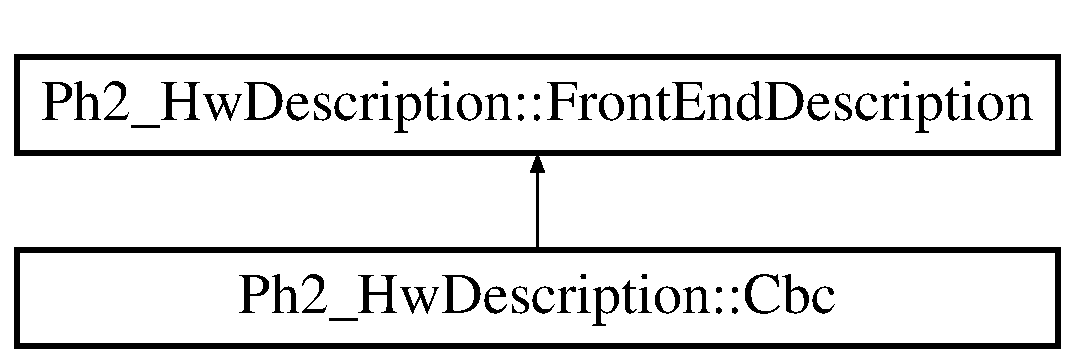
\includegraphics[height=2.000000cm]{class_ph2___hw_description_1_1_cbc}
\end{center}
\end{figure}
\subsection*{Public Member Functions}
\begin{DoxyCompactItemize}
\item 
\hyperlink{class_ph2___hw_description_1_1_cbc_a4569a0838d600c2d96f25adb6403e610}{Cbc} (\hyperlink{class_ph2___hw_description_1_1_f_e_description}{F\-E\-Description} \&p\-Fe\-Desc, uint8\-\_\-t p\-Cbc\-Id, std\-::string filename)
\item 
\hyperlink{class_ph2___hw_description_1_1_cbc_a8ad3757886613841f563b6eecd5d8406}{Cbc} (\hyperlink{class_ph2___hw_description_1_1_f_e_description}{F\-E\-Description} \&p\-Fe\-Desc, uint8\-\_\-t p\-Cbc\-Id, uint8\-\_\-t p\-Trigger\-Latency, uint8\-\_\-t p\-Vcth)
\item 
\hyperlink{class_ph2___hw_description_1_1_cbc_ad14c3944426f98d07914d0cb0fd38948}{Cbc} (\hyperlink{class_ph2___hw_description_1_1_f_e_description}{F\-E\-Description} \&p\-Fe\-Desc, uint8\-\_\-t p\-Cbc\-Id)
\item 
\hyperlink{class_ph2___hw_description_1_1_cbc_ad2ec420b5bd8e361a151b585a62c0ebe}{Cbc} (uint8\-\_\-t p\-Shelve\-Id, uint8\-\_\-t p\-Be\-Id, uint8\-\_\-t p\-F\-M\-C\-Id, uint8\-\_\-t p\-Fe\-Id, uint8\-\_\-t p\-Cbc\-Id, std\-::string filename)
\item 
\hyperlink{class_ph2___hw_description_1_1_cbc_a31698ad31b2484c74b87647e9451fc6d}{Cbc} (uint8\-\_\-t p\-Shelve\-Id, uint8\-\_\-t p\-Be\-Id, uint8\-\_\-t p\-F\-M\-C\-Id, uint8\-\_\-t p\-Fe\-Id, uint8\-\_\-t p\-Cbc\-Id, uint8\-\_\-t p\-Trigger\-Latency, uint8\-\_\-t p\-Vcth)
\item 
\hyperlink{class_ph2___hw_description_1_1_cbc_ac7e237f12e6950b45538e3706be11bb0}{Cbc} (uint8\-\_\-t p\-Shelve\-Id, uint8\-\_\-t p\-Be\-Id, uint8\-\_\-t p\-F\-M\-C\-Id, uint8\-\_\-t p\-Fe\-Id, uint8\-\_\-t p\-Cbc\-Id)
\item 
\hyperlink{class_ph2___hw_description_1_1_cbc_a5b7124456823871d611ada17ed0a51a1}{Cbc} ()
\item 
\hyperlink{class_ph2___hw_description_1_1_cbc_ab529cbb8cbbbc3b28a7ca2a472d4aa50}{Cbc} (const \hyperlink{class_ph2___hw_description_1_1_cbc}{Cbc} \&cbcobj)
\item 
\hyperlink{class_ph2___hw_description_1_1_cbc_a4e641d292073978e6e1b34fa91c13067}{$\sim$\-Cbc} ()
\item 
void \hyperlink{class_ph2___hw_description_1_1_cbc_afd6fdbe40eff3c160221a3a8acfb657d}{loadf\-Reg\-Map} (std\-::string filename)
\begin{DoxyCompactList}\small\item\em Load Reg\-Map from a file. \end{DoxyCompactList}\item 
uint8\-\_\-t \hyperlink{class_ph2___hw_description_1_1_cbc_a7dcee2bd6f0cbe1e9342f4d8e4229477}{get\-Trigger\-Latency} ()
\begin{DoxyCompactList}\small\item\em Get the register Trigger\-Latency from the Map. \end{DoxyCompactList}\item 
void \hyperlink{class_ph2___hw_description_1_1_cbc_af2ca8a515be91e594345f59765eedc86}{set\-Trigger\-Latency} (uint8\-\_\-t p\-Trigger\-Latency)
\begin{DoxyCompactList}\small\item\em Set the register Trigger\-Latency of the Map. \end{DoxyCompactList}\item 
uint8\-\_\-t \hyperlink{class_ph2___hw_description_1_1_cbc_ad52630f4caa9defc0c46e38c7f828d5f}{get\-Vcth} ()
\begin{DoxyCompactList}\small\item\em Get the register Vcth from the Map. \end{DoxyCompactList}\item 
void \hyperlink{class_ph2___hw_description_1_1_cbc_a055db371622ef5e565d7abd490d1b5bd}{set\-Vcth} (uint8\-\_\-t pset\-Vcth)
\begin{DoxyCompactList}\small\item\em Set the register Vcth of the Map. \end{DoxyCompactList}\item 
uint8\-\_\-t \hyperlink{class_ph2___hw_description_1_1_cbc_a8e29ea3bf86977585b3824941d948f91}{get\-Reg} (std\-::string p\-Reg)
\begin{DoxyCompactList}\small\item\em Get any register from the Map. \end{DoxyCompactList}\item 
void \hyperlink{class_ph2___hw_description_1_1_cbc_aa24292fe56d6b19ec08ba67f9790b5c7}{set\-Reg} (std\-::string p\-Reg, uint8\-\_\-t pset\-Value)
\begin{DoxyCompactList}\small\item\em Set any register of the Map. \end{DoxyCompactList}\item 
void \hyperlink{class_ph2___hw_description_1_1_cbc_a21a95937ae871d154b4d0f7f2fe6bd02}{write\-Reg\-Values} (std\-::string filename)
\begin{DoxyCompactList}\small\item\em Write the registers of the Map in a file. \end{DoxyCompactList}\item 
uint8\-\_\-t \hyperlink{class_ph2___hw_description_1_1_cbc_a14a78f27fb0e6c74622b6bc49259a2f3}{get\-Cbc\-Id} ()
\begin{DoxyCompactList}\small\item\em Get the \hyperlink{class_ph2___hw_description_1_1_cbc}{Cbc} Id. \end{DoxyCompactList}\item 
\hyperlink{namespace_ph2___hw_description_a9a23b373068f169aa67ca1d22c9a6001}{Cbc\-Reg\-Map} \hyperlink{class_ph2___hw_description_1_1_cbc_ad2bae647b2474b4737d7f2ede5a73ed3}{get\-Reg\-Map} ()
\begin{DoxyCompactList}\small\item\em Get the Map of the registers. \end{DoxyCompactList}\end{DoxyCompactItemize}
\subsection*{Data Fields}
\begin{DoxyCompactItemize}
\item 
uint8\-\_\-t \hyperlink{class_ph2___hw_description_1_1_cbc_a99b392306d4cdb7ffa7f956fc553011c}{f\-Cbc\-Id}
\end{DoxyCompactItemize}
\subsection*{Protected Attributes}
\begin{DoxyCompactItemize}
\item 
\hyperlink{namespace_ph2___hw_description_a9a23b373068f169aa67ca1d22c9a6001}{Cbc\-Reg\-Map} \hyperlink{class_ph2___hw_description_1_1_cbc_ab4dbf1af172e821d95f77acb7e4fb962}{f\-Reg\-Map}
\end{DoxyCompactItemize}


\subsection{Detailed Description}
Read/\-Write \hyperlink{class_ph2___hw_description_1_1_cbc}{Cbc}'s registers on a file. 

\subsection{Constructor \& Destructor Documentation}
\hypertarget{class_ph2___hw_description_1_1_cbc_a4569a0838d600c2d96f25adb6403e610}{\index{Ph2\-\_\-\-Hw\-Description\-::\-Cbc@{Ph2\-\_\-\-Hw\-Description\-::\-Cbc}!Cbc@{Cbc}}
\index{Cbc@{Cbc}!Ph2_HwDescription::Cbc@{Ph2\-\_\-\-Hw\-Description\-::\-Cbc}}
\subsubsection[{Cbc}]{\setlength{\rightskip}{0pt plus 5cm}Ph2\-\_\-\-Hw\-Description\-::\-Cbc\-::\-Cbc (
\begin{DoxyParamCaption}
\item[{{\bf F\-E\-Description} \&}]{p\-Fe\-Desc, }
\item[{uint8\-\_\-t}]{p\-Cbc\-Id, }
\item[{std\-::string}]{filename}
\end{DoxyParamCaption}
)}}\label{class_ph2___hw_description_1_1_cbc_a4569a0838d600c2d96f25adb6403e610}
\hypertarget{class_ph2___hw_description_1_1_cbc_a8ad3757886613841f563b6eecd5d8406}{\index{Ph2\-\_\-\-Hw\-Description\-::\-Cbc@{Ph2\-\_\-\-Hw\-Description\-::\-Cbc}!Cbc@{Cbc}}
\index{Cbc@{Cbc}!Ph2_HwDescription::Cbc@{Ph2\-\_\-\-Hw\-Description\-::\-Cbc}}
\subsubsection[{Cbc}]{\setlength{\rightskip}{0pt plus 5cm}Ph2\-\_\-\-Hw\-Description\-::\-Cbc\-::\-Cbc (
\begin{DoxyParamCaption}
\item[{{\bf F\-E\-Description} \&}]{p\-Fe\-Desc, }
\item[{uint8\-\_\-t}]{p\-Cbc\-Id, }
\item[{uint8\-\_\-t}]{p\-Trigger\-Latency, }
\item[{uint8\-\_\-t}]{p\-Vcth}
\end{DoxyParamCaption}
)}}\label{class_ph2___hw_description_1_1_cbc_a8ad3757886613841f563b6eecd5d8406}
\hypertarget{class_ph2___hw_description_1_1_cbc_ad14c3944426f98d07914d0cb0fd38948}{\index{Ph2\-\_\-\-Hw\-Description\-::\-Cbc@{Ph2\-\_\-\-Hw\-Description\-::\-Cbc}!Cbc@{Cbc}}
\index{Cbc@{Cbc}!Ph2_HwDescription::Cbc@{Ph2\-\_\-\-Hw\-Description\-::\-Cbc}}
\subsubsection[{Cbc}]{\setlength{\rightskip}{0pt plus 5cm}Ph2\-\_\-\-Hw\-Description\-::\-Cbc\-::\-Cbc (
\begin{DoxyParamCaption}
\item[{{\bf F\-E\-Description} \&}]{p\-Fe\-Desc, }
\item[{uint8\-\_\-t}]{p\-Cbc\-Id}
\end{DoxyParamCaption}
)}}\label{class_ph2___hw_description_1_1_cbc_ad14c3944426f98d07914d0cb0fd38948}
\hypertarget{class_ph2___hw_description_1_1_cbc_ad2ec420b5bd8e361a151b585a62c0ebe}{\index{Ph2\-\_\-\-Hw\-Description\-::\-Cbc@{Ph2\-\_\-\-Hw\-Description\-::\-Cbc}!Cbc@{Cbc}}
\index{Cbc@{Cbc}!Ph2_HwDescription::Cbc@{Ph2\-\_\-\-Hw\-Description\-::\-Cbc}}
\subsubsection[{Cbc}]{\setlength{\rightskip}{0pt plus 5cm}Ph2\-\_\-\-Hw\-Description\-::\-Cbc\-::\-Cbc (
\begin{DoxyParamCaption}
\item[{uint8\-\_\-t}]{p\-Shelve\-Id, }
\item[{uint8\-\_\-t}]{p\-Be\-Id, }
\item[{uint8\-\_\-t}]{p\-F\-M\-C\-Id, }
\item[{uint8\-\_\-t}]{p\-Fe\-Id, }
\item[{uint8\-\_\-t}]{p\-Cbc\-Id, }
\item[{std\-::string}]{filename}
\end{DoxyParamCaption}
)}}\label{class_ph2___hw_description_1_1_cbc_ad2ec420b5bd8e361a151b585a62c0ebe}
\hypertarget{class_ph2___hw_description_1_1_cbc_a31698ad31b2484c74b87647e9451fc6d}{\index{Ph2\-\_\-\-Hw\-Description\-::\-Cbc@{Ph2\-\_\-\-Hw\-Description\-::\-Cbc}!Cbc@{Cbc}}
\index{Cbc@{Cbc}!Ph2_HwDescription::Cbc@{Ph2\-\_\-\-Hw\-Description\-::\-Cbc}}
\subsubsection[{Cbc}]{\setlength{\rightskip}{0pt plus 5cm}Ph2\-\_\-\-Hw\-Description\-::\-Cbc\-::\-Cbc (
\begin{DoxyParamCaption}
\item[{uint8\-\_\-t}]{p\-Shelve\-Id, }
\item[{uint8\-\_\-t}]{p\-Be\-Id, }
\item[{uint8\-\_\-t}]{p\-F\-M\-C\-Id, }
\item[{uint8\-\_\-t}]{p\-Fe\-Id, }
\item[{uint8\-\_\-t}]{p\-Cbc\-Id, }
\item[{uint8\-\_\-t}]{p\-Trigger\-Latency, }
\item[{uint8\-\_\-t}]{p\-Vcth}
\end{DoxyParamCaption}
)}}\label{class_ph2___hw_description_1_1_cbc_a31698ad31b2484c74b87647e9451fc6d}
\hypertarget{class_ph2___hw_description_1_1_cbc_ac7e237f12e6950b45538e3706be11bb0}{\index{Ph2\-\_\-\-Hw\-Description\-::\-Cbc@{Ph2\-\_\-\-Hw\-Description\-::\-Cbc}!Cbc@{Cbc}}
\index{Cbc@{Cbc}!Ph2_HwDescription::Cbc@{Ph2\-\_\-\-Hw\-Description\-::\-Cbc}}
\subsubsection[{Cbc}]{\setlength{\rightskip}{0pt plus 5cm}Ph2\-\_\-\-Hw\-Description\-::\-Cbc\-::\-Cbc (
\begin{DoxyParamCaption}
\item[{uint8\-\_\-t}]{p\-Shelve\-Id, }
\item[{uint8\-\_\-t}]{p\-Be\-Id, }
\item[{uint8\-\_\-t}]{p\-F\-M\-C\-Id, }
\item[{uint8\-\_\-t}]{p\-Fe\-Id, }
\item[{uint8\-\_\-t}]{p\-Cbc\-Id}
\end{DoxyParamCaption}
)}}\label{class_ph2___hw_description_1_1_cbc_ac7e237f12e6950b45538e3706be11bb0}
\hypertarget{class_ph2___hw_description_1_1_cbc_a5b7124456823871d611ada17ed0a51a1}{\index{Ph2\-\_\-\-Hw\-Description\-::\-Cbc@{Ph2\-\_\-\-Hw\-Description\-::\-Cbc}!Cbc@{Cbc}}
\index{Cbc@{Cbc}!Ph2_HwDescription::Cbc@{Ph2\-\_\-\-Hw\-Description\-::\-Cbc}}
\subsubsection[{Cbc}]{\setlength{\rightskip}{0pt plus 5cm}Ph2\-\_\-\-Hw\-Description\-::\-Cbc\-::\-Cbc (
\begin{DoxyParamCaption}
{}
\end{DoxyParamCaption}
)}}\label{class_ph2___hw_description_1_1_cbc_a5b7124456823871d611ada17ed0a51a1}
\hypertarget{class_ph2___hw_description_1_1_cbc_ab529cbb8cbbbc3b28a7ca2a472d4aa50}{\index{Ph2\-\_\-\-Hw\-Description\-::\-Cbc@{Ph2\-\_\-\-Hw\-Description\-::\-Cbc}!Cbc@{Cbc}}
\index{Cbc@{Cbc}!Ph2_HwDescription::Cbc@{Ph2\-\_\-\-Hw\-Description\-::\-Cbc}}
\subsubsection[{Cbc}]{\setlength{\rightskip}{0pt plus 5cm}Ph2\-\_\-\-Hw\-Description\-::\-Cbc\-::\-Cbc (
\begin{DoxyParamCaption}
\item[{const {\bf Cbc} \&}]{cbcobj}
\end{DoxyParamCaption}
)}}\label{class_ph2___hw_description_1_1_cbc_ab529cbb8cbbbc3b28a7ca2a472d4aa50}
\hypertarget{class_ph2___hw_description_1_1_cbc_a4e641d292073978e6e1b34fa91c13067}{\index{Ph2\-\_\-\-Hw\-Description\-::\-Cbc@{Ph2\-\_\-\-Hw\-Description\-::\-Cbc}!$\sim$\-Cbc@{$\sim$\-Cbc}}
\index{$\sim$\-Cbc@{$\sim$\-Cbc}!Ph2_HwDescription::Cbc@{Ph2\-\_\-\-Hw\-Description\-::\-Cbc}}
\subsubsection[{$\sim$\-Cbc}]{\setlength{\rightskip}{0pt plus 5cm}Ph2\-\_\-\-Hw\-Description\-::\-Cbc\-::$\sim$\-Cbc (
\begin{DoxyParamCaption}
{}
\end{DoxyParamCaption}
)}}\label{class_ph2___hw_description_1_1_cbc_a4e641d292073978e6e1b34fa91c13067}


\subsection{Member Function Documentation}
\hypertarget{class_ph2___hw_description_1_1_cbc_a14a78f27fb0e6c74622b6bc49259a2f3}{\index{Ph2\-\_\-\-Hw\-Description\-::\-Cbc@{Ph2\-\_\-\-Hw\-Description\-::\-Cbc}!get\-Cbc\-Id@{get\-Cbc\-Id}}
\index{get\-Cbc\-Id@{get\-Cbc\-Id}!Ph2_HwDescription::Cbc@{Ph2\-\_\-\-Hw\-Description\-::\-Cbc}}
\subsubsection[{get\-Cbc\-Id}]{\setlength{\rightskip}{0pt plus 5cm}uint8\-\_\-t Ph2\-\_\-\-Hw\-Description\-::\-Cbc\-::get\-Cbc\-Id (
\begin{DoxyParamCaption}
{}
\end{DoxyParamCaption}
)\hspace{0.3cm}{\ttfamily [inline]}}}\label{class_ph2___hw_description_1_1_cbc_a14a78f27fb0e6c74622b6bc49259a2f3}


Get the \hyperlink{class_ph2___hw_description_1_1_cbc}{Cbc} Id. 

\begin{DoxyReturn}{Returns}
The \hyperlink{class_ph2___hw_description_1_1_cbc}{Cbc} I\-D 
\end{DoxyReturn}
\hypertarget{class_ph2___hw_description_1_1_cbc_a8e29ea3bf86977585b3824941d948f91}{\index{Ph2\-\_\-\-Hw\-Description\-::\-Cbc@{Ph2\-\_\-\-Hw\-Description\-::\-Cbc}!get\-Reg@{get\-Reg}}
\index{get\-Reg@{get\-Reg}!Ph2_HwDescription::Cbc@{Ph2\-\_\-\-Hw\-Description\-::\-Cbc}}
\subsubsection[{get\-Reg}]{\setlength{\rightskip}{0pt plus 5cm}uint8\-\_\-t Ph2\-\_\-\-Hw\-Description\-::\-Cbc\-::get\-Reg (
\begin{DoxyParamCaption}
\item[{std\-::string}]{p\-Reg}
\end{DoxyParamCaption}
)}}\label{class_ph2___hw_description_1_1_cbc_a8e29ea3bf86977585b3824941d948f91}


Get any register from the Map. 


\begin{DoxyParams}{Parameters}
{\em p\-Reg} & \\
\hline
\end{DoxyParams}
\begin{DoxyReturn}{Returns}
The value of the register 
\end{DoxyReturn}
\hypertarget{class_ph2___hw_description_1_1_cbc_ad2bae647b2474b4737d7f2ede5a73ed3}{\index{Ph2\-\_\-\-Hw\-Description\-::\-Cbc@{Ph2\-\_\-\-Hw\-Description\-::\-Cbc}!get\-Reg\-Map@{get\-Reg\-Map}}
\index{get\-Reg\-Map@{get\-Reg\-Map}!Ph2_HwDescription::Cbc@{Ph2\-\_\-\-Hw\-Description\-::\-Cbc}}
\subsubsection[{get\-Reg\-Map}]{\setlength{\rightskip}{0pt plus 5cm}{\bf Cbc\-Reg\-Map} Ph2\-\_\-\-Hw\-Description\-::\-Cbc\-::get\-Reg\-Map (
\begin{DoxyParamCaption}
{}
\end{DoxyParamCaption}
)\hspace{0.3cm}{\ttfamily [inline]}}}\label{class_ph2___hw_description_1_1_cbc_ad2bae647b2474b4737d7f2ede5a73ed3}


Get the Map of the registers. 

\begin{DoxyReturn}{Returns}
The map of register 
\end{DoxyReturn}
\hypertarget{class_ph2___hw_description_1_1_cbc_a7dcee2bd6f0cbe1e9342f4d8e4229477}{\index{Ph2\-\_\-\-Hw\-Description\-::\-Cbc@{Ph2\-\_\-\-Hw\-Description\-::\-Cbc}!get\-Trigger\-Latency@{get\-Trigger\-Latency}}
\index{get\-Trigger\-Latency@{get\-Trigger\-Latency}!Ph2_HwDescription::Cbc@{Ph2\-\_\-\-Hw\-Description\-::\-Cbc}}
\subsubsection[{get\-Trigger\-Latency}]{\setlength{\rightskip}{0pt plus 5cm}uint8\-\_\-t Ph2\-\_\-\-Hw\-Description\-::\-Cbc\-::get\-Trigger\-Latency (
\begin{DoxyParamCaption}
{}
\end{DoxyParamCaption}
)}}\label{class_ph2___hw_description_1_1_cbc_a7dcee2bd6f0cbe1e9342f4d8e4229477}


Get the register Trigger\-Latency from the Map. 

\begin{DoxyReturn}{Returns}
The value of Trigger\-Lantency 
\end{DoxyReturn}
\hypertarget{class_ph2___hw_description_1_1_cbc_ad52630f4caa9defc0c46e38c7f828d5f}{\index{Ph2\-\_\-\-Hw\-Description\-::\-Cbc@{Ph2\-\_\-\-Hw\-Description\-::\-Cbc}!get\-Vcth@{get\-Vcth}}
\index{get\-Vcth@{get\-Vcth}!Ph2_HwDescription::Cbc@{Ph2\-\_\-\-Hw\-Description\-::\-Cbc}}
\subsubsection[{get\-Vcth}]{\setlength{\rightskip}{0pt plus 5cm}uint8\-\_\-t Ph2\-\_\-\-Hw\-Description\-::\-Cbc\-::get\-Vcth (
\begin{DoxyParamCaption}
{}
\end{DoxyParamCaption}
)}}\label{class_ph2___hw_description_1_1_cbc_ad52630f4caa9defc0c46e38c7f828d5f}


Get the register Vcth from the Map. 

\begin{DoxyReturn}{Returns}
The value of Vcth 
\end{DoxyReturn}
\hypertarget{class_ph2___hw_description_1_1_cbc_afd6fdbe40eff3c160221a3a8acfb657d}{\index{Ph2\-\_\-\-Hw\-Description\-::\-Cbc@{Ph2\-\_\-\-Hw\-Description\-::\-Cbc}!loadf\-Reg\-Map@{loadf\-Reg\-Map}}
\index{loadf\-Reg\-Map@{loadf\-Reg\-Map}!Ph2_HwDescription::Cbc@{Ph2\-\_\-\-Hw\-Description\-::\-Cbc}}
\subsubsection[{loadf\-Reg\-Map}]{\setlength{\rightskip}{0pt plus 5cm}void Ph2\-\_\-\-Hw\-Description\-::\-Cbc\-::loadf\-Reg\-Map (
\begin{DoxyParamCaption}
\item[{std\-::string}]{filename}
\end{DoxyParamCaption}
)}}\label{class_ph2___hw_description_1_1_cbc_afd6fdbe40eff3c160221a3a8acfb657d}


Load Reg\-Map from a file. 


\begin{DoxyParams}{Parameters}
{\em filename} & \\
\hline
\end{DoxyParams}
\hypertarget{class_ph2___hw_description_1_1_cbc_aa24292fe56d6b19ec08ba67f9790b5c7}{\index{Ph2\-\_\-\-Hw\-Description\-::\-Cbc@{Ph2\-\_\-\-Hw\-Description\-::\-Cbc}!set\-Reg@{set\-Reg}}
\index{set\-Reg@{set\-Reg}!Ph2_HwDescription::Cbc@{Ph2\-\_\-\-Hw\-Description\-::\-Cbc}}
\subsubsection[{set\-Reg}]{\setlength{\rightskip}{0pt plus 5cm}void Ph2\-\_\-\-Hw\-Description\-::\-Cbc\-::set\-Reg (
\begin{DoxyParamCaption}
\item[{std\-::string}]{p\-Reg, }
\item[{uint8\-\_\-t}]{pset\-Value}
\end{DoxyParamCaption}
)}}\label{class_ph2___hw_description_1_1_cbc_aa24292fe56d6b19ec08ba67f9790b5c7}


Set any register of the Map. 


\begin{DoxyParams}{Parameters}
{\em p\-Reg} & \\
\hline
{\em pset\-Value} & \\
\hline
\end{DoxyParams}
\hypertarget{class_ph2___hw_description_1_1_cbc_af2ca8a515be91e594345f59765eedc86}{\index{Ph2\-\_\-\-Hw\-Description\-::\-Cbc@{Ph2\-\_\-\-Hw\-Description\-::\-Cbc}!set\-Trigger\-Latency@{set\-Trigger\-Latency}}
\index{set\-Trigger\-Latency@{set\-Trigger\-Latency}!Ph2_HwDescription::Cbc@{Ph2\-\_\-\-Hw\-Description\-::\-Cbc}}
\subsubsection[{set\-Trigger\-Latency}]{\setlength{\rightskip}{0pt plus 5cm}void Ph2\-\_\-\-Hw\-Description\-::\-Cbc\-::set\-Trigger\-Latency (
\begin{DoxyParamCaption}
\item[{uint8\-\_\-t}]{p\-Trigger\-Latency}
\end{DoxyParamCaption}
)}}\label{class_ph2___hw_description_1_1_cbc_af2ca8a515be91e594345f59765eedc86}


Set the register Trigger\-Latency of the Map. 


\begin{DoxyParams}{Parameters}
{\em p\-Trigger\-Latency} & \\
\hline
\end{DoxyParams}
\hypertarget{class_ph2___hw_description_1_1_cbc_a055db371622ef5e565d7abd490d1b5bd}{\index{Ph2\-\_\-\-Hw\-Description\-::\-Cbc@{Ph2\-\_\-\-Hw\-Description\-::\-Cbc}!set\-Vcth@{set\-Vcth}}
\index{set\-Vcth@{set\-Vcth}!Ph2_HwDescription::Cbc@{Ph2\-\_\-\-Hw\-Description\-::\-Cbc}}
\subsubsection[{set\-Vcth}]{\setlength{\rightskip}{0pt plus 5cm}void Ph2\-\_\-\-Hw\-Description\-::\-Cbc\-::set\-Vcth (
\begin{DoxyParamCaption}
\item[{uint8\-\_\-t}]{pset\-Vcth}
\end{DoxyParamCaption}
)}}\label{class_ph2___hw_description_1_1_cbc_a055db371622ef5e565d7abd490d1b5bd}


Set the register Vcth of the Map. 


\begin{DoxyParams}{Parameters}
{\em pset\-Vcth} & \\
\hline
\end{DoxyParams}
\hypertarget{class_ph2___hw_description_1_1_cbc_a21a95937ae871d154b4d0f7f2fe6bd02}{\index{Ph2\-\_\-\-Hw\-Description\-::\-Cbc@{Ph2\-\_\-\-Hw\-Description\-::\-Cbc}!write\-Reg\-Values@{write\-Reg\-Values}}
\index{write\-Reg\-Values@{write\-Reg\-Values}!Ph2_HwDescription::Cbc@{Ph2\-\_\-\-Hw\-Description\-::\-Cbc}}
\subsubsection[{write\-Reg\-Values}]{\setlength{\rightskip}{0pt plus 5cm}void Ph2\-\_\-\-Hw\-Description\-::\-Cbc\-::write\-Reg\-Values (
\begin{DoxyParamCaption}
\item[{std\-::string}]{filename}
\end{DoxyParamCaption}
)}}\label{class_ph2___hw_description_1_1_cbc_a21a95937ae871d154b4d0f7f2fe6bd02}


Write the registers of the Map in a file. 


\begin{DoxyParams}{Parameters}
{\em filename} & \\
\hline
\end{DoxyParams}


\subsection{Field Documentation}
\hypertarget{class_ph2___hw_description_1_1_cbc_a99b392306d4cdb7ffa7f956fc553011c}{\index{Ph2\-\_\-\-Hw\-Description\-::\-Cbc@{Ph2\-\_\-\-Hw\-Description\-::\-Cbc}!f\-Cbc\-Id@{f\-Cbc\-Id}}
\index{f\-Cbc\-Id@{f\-Cbc\-Id}!Ph2_HwDescription::Cbc@{Ph2\-\_\-\-Hw\-Description\-::\-Cbc}}
\subsubsection[{f\-Cbc\-Id}]{\setlength{\rightskip}{0pt plus 5cm}uint8\-\_\-t Ph2\-\_\-\-Hw\-Description\-::\-Cbc\-::f\-Cbc\-Id}}\label{class_ph2___hw_description_1_1_cbc_a99b392306d4cdb7ffa7f956fc553011c}
\hypertarget{class_ph2___hw_description_1_1_cbc_ab4dbf1af172e821d95f77acb7e4fb962}{\index{Ph2\-\_\-\-Hw\-Description\-::\-Cbc@{Ph2\-\_\-\-Hw\-Description\-::\-Cbc}!f\-Reg\-Map@{f\-Reg\-Map}}
\index{f\-Reg\-Map@{f\-Reg\-Map}!Ph2_HwDescription::Cbc@{Ph2\-\_\-\-Hw\-Description\-::\-Cbc}}
\subsubsection[{f\-Reg\-Map}]{\setlength{\rightskip}{0pt plus 5cm}{\bf Cbc\-Reg\-Map} Ph2\-\_\-\-Hw\-Description\-::\-Cbc\-::f\-Reg\-Map\hspace{0.3cm}{\ttfamily [protected]}}}\label{class_ph2___hw_description_1_1_cbc_ab4dbf1af172e821d95f77acb7e4fb962}


The documentation for this class was generated from the following files\-:\begin{DoxyCompactItemize}
\item 
H\-W\-Description/\hyperlink{_cbc_8h}{Cbc.\-h}\item 
H\-W\-Description/\hyperlink{_cbc_8cc}{Cbc.\-cc}\end{DoxyCompactItemize}

\hypertarget{struct_ph2___hw_description_1_1_cbc_comparer}{\section{Ph2\-\_\-\-Hw\-Description\-:\-:Cbc\-Comparer Struct Reference}
\label{struct_ph2___hw_description_1_1_cbc_comparer}\index{Ph2\-\_\-\-Hw\-Description\-::\-Cbc\-Comparer@{Ph2\-\_\-\-Hw\-Description\-::\-Cbc\-Comparer}}
}


Compare two \hyperlink{class_ph2___hw_description_1_1_cbc}{Cbc} by their I\-D.  




{\ttfamily \#include $<$Cbc.\-h$>$}

\subsection*{Public Member Functions}
\begin{DoxyCompactItemize}
\item 
bool \hyperlink{struct_ph2___hw_description_1_1_cbc_comparer_af83d2c46bcdcb36adcd0ae91f929942a}{operator()} (\hyperlink{class_ph2___hw_description_1_1_cbc}{Cbc} \&cbc1, \hyperlink{class_ph2___hw_description_1_1_cbc}{Cbc} \&cbc2)
\end{DoxyCompactItemize}


\subsection{Detailed Description}
Compare two \hyperlink{class_ph2___hw_description_1_1_cbc}{Cbc} by their I\-D. 

\subsection{Member Function Documentation}
\hypertarget{struct_ph2___hw_description_1_1_cbc_comparer_af83d2c46bcdcb36adcd0ae91f929942a}{\index{Ph2\-\_\-\-Hw\-Description\-::\-Cbc\-Comparer@{Ph2\-\_\-\-Hw\-Description\-::\-Cbc\-Comparer}!operator()@{operator()}}
\index{operator()@{operator()}!Ph2_HwDescription::CbcComparer@{Ph2\-\_\-\-Hw\-Description\-::\-Cbc\-Comparer}}
\subsubsection[{operator()}]{\setlength{\rightskip}{0pt plus 5cm}bool Ph2\-\_\-\-Hw\-Description\-::\-Cbc\-Comparer\-::operator() (
\begin{DoxyParamCaption}
\item[{{\bf Cbc} \&}]{cbc1, }
\item[{{\bf Cbc} \&}]{cbc2}
\end{DoxyParamCaption}
)}}\label{struct_ph2___hw_description_1_1_cbc_comparer_af83d2c46bcdcb36adcd0ae91f929942a}


The documentation for this struct was generated from the following files\-:\begin{DoxyCompactItemize}
\item 
H\-W\-Description/\hyperlink{_cbc_8h}{Cbc.\-h}\item 
H\-W\-Description/\hyperlink{_cbc_8cc}{Cbc.\-cc}\end{DoxyCompactItemize}

\hypertarget{class_ph2___hw_interface_1_1_cbc_interface}{\section{Ph2\-\_\-\-Hw\-Interface\-:\-:Cbc\-Interface Class Reference}
\label{class_ph2___hw_interface_1_1_cbc_interface}\index{Ph2\-\_\-\-Hw\-Interface\-::\-Cbc\-Interface@{Ph2\-\_\-\-Hw\-Interface\-::\-Cbc\-Interface}}
}
Inheritance diagram for Ph2\-\_\-\-Hw\-Interface\-:\-:Cbc\-Interface\-:\begin{figure}[H]
\begin{center}
\leavevmode
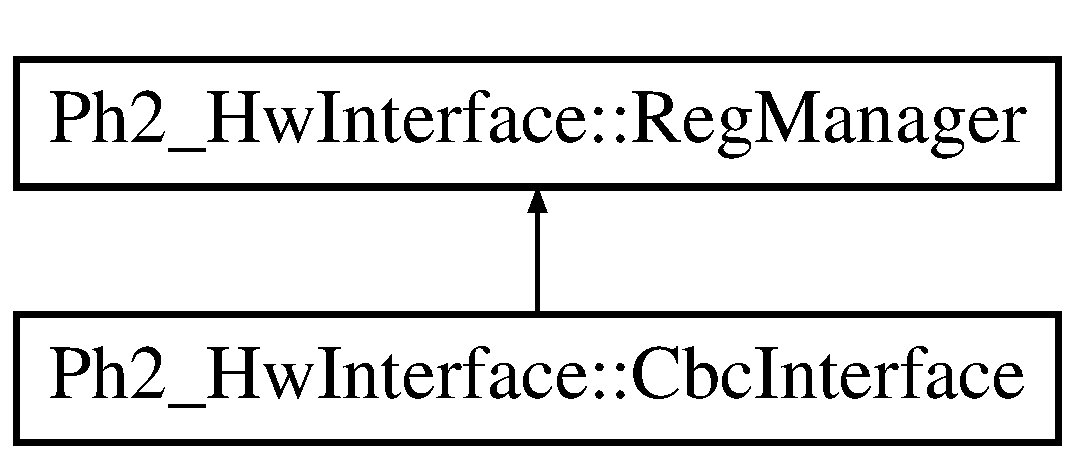
\includegraphics[height=2.000000cm]{class_ph2___hw_interface_1_1_cbc_interface}
\end{center}
\end{figure}
\subsection*{Public Member Functions}
\begin{DoxyCompactItemize}
\item 
\hypertarget{class_ph2___hw_interface_1_1_cbc_interface_a3ddefe5549da06a7d26fee1502a792b4}{{\bfseries Cbc\-Interface} (const char $\ast$pu\-Hal\-Config\-File\-Name)}\label{class_ph2___hw_interface_1_1_cbc_interface_a3ddefe5549da06a7d26fee1502a792b4}

\item 
\hypertarget{class_ph2___hw_interface_1_1_cbc_interface_af5cf4eb5b7134835f00349cb19f35c56}{void \hyperlink{class_ph2___hw_interface_1_1_cbc_interface_af5cf4eb5b7134835f00349cb19f35c56}{Configure\-Cbc} (Cbc \&p\-Cbc)}\label{class_ph2___hw_interface_1_1_cbc_interface_af5cf4eb5b7134835f00349cb19f35c56}

\begin{DoxyCompactList}\small\item\em Configure the Cbc after the Cbc\-Config\-File. \end{DoxyCompactList}\item 
\hypertarget{class_ph2___hw_interface_1_1_cbc_interface_a498d71b5709e0524b8e9dc50b92d1424}{void \hyperlink{class_ph2___hw_interface_1_1_cbc_interface_a498d71b5709e0524b8e9dc50b92d1424}{Update\-Cbc\-Write} (Cbc \&p\-Cbc, const std\-::string \&p\-Reg\-Node, uint32\-\_\-t \&p\-Word)}\label{class_ph2___hw_interface_1_1_cbc_interface_a498d71b5709e0524b8e9dc50b92d1424}

\begin{DoxyCompactList}\small\item\em Write the designated register in both Cbc and Cbc\-Config\-File. \end{DoxyCompactList}\item 
\hypertarget{class_ph2___hw_interface_1_1_cbc_interface_ab08ea1de98fe120098a4f5c52e017393}{void \hyperlink{class_ph2___hw_interface_1_1_cbc_interface_ab08ea1de98fe120098a4f5c52e017393}{Update\-Cbc\-Read} (Cbc \&p\-Cbc, const std\-::string \&p\-Reg\-Node)}\label{class_ph2___hw_interface_1_1_cbc_interface_ab08ea1de98fe120098a4f5c52e017393}

\begin{DoxyCompactList}\small\item\em Read the designated register in the Cbc and update the Cbc\-Config\-File. \end{DoxyCompactList}\end{DoxyCompactItemize}
\subsection*{Static Public Attributes}
\begin{DoxyCompactItemize}
\item 
\hypertarget{class_ph2___hw_interface_1_1_cbc_interface_ab45dcb5563c94075ac0a3e17d17c1fd4}{static const std\-::string {\bfseries f\-Str\-I2c\-Settings} = I2\-C\-\_\-\-S\-E\-T\-T\-I\-N\-G\-S}\label{class_ph2___hw_interface_1_1_cbc_interface_ab45dcb5563c94075ac0a3e17d17c1fd4}

\item 
\hypertarget{class_ph2___hw_interface_1_1_cbc_interface_a350e32baca2a50220eeff24b9fa07054}{static const std\-::string {\bfseries f\-Str\-I2c\-Command} = I2\-C\-\_\-\-C\-O\-M\-M\-A\-N\-D}\label{class_ph2___hw_interface_1_1_cbc_interface_a350e32baca2a50220eeff24b9fa07054}

\item 
\hypertarget{class_ph2___hw_interface_1_1_cbc_interface_a6a0730099e121a7707615ba6969afe80}{static const std\-::string {\bfseries f\-Str\-I2c\-Reply} = I2\-C\-\_\-\-R\-E\-P\-L\-Y}\label{class_ph2___hw_interface_1_1_cbc_interface_a6a0730099e121a7707615ba6969afe80}

\item 
\hypertarget{class_ph2___hw_interface_1_1_cbc_interface_ad5257bb9fac0efe9cb8307a04f51ef77}{static const uint32\-\_\-t {\bfseries f\-I2c\-Slave} = I2\-C\-\_\-\-S\-L\-A\-V\-E}\label{class_ph2___hw_interface_1_1_cbc_interface_ad5257bb9fac0efe9cb8307a04f51ef77}

\end{DoxyCompactItemize}
\subsection*{Additional Inherited Members}


The documentation for this class was generated from the following files\-:\begin{DoxyCompactItemize}
\item 
Cbc\-Interface.\-h\item 
Cbc\-Interface.\-cc\end{DoxyCompactItemize}

\hypertarget{struct_ph2___hw_description_1_1_cbc_reg_item}{\section{Ph2\-\_\-\-Hw\-Description\-:\-:Cbc\-Reg\-Item Struct Reference}
\label{struct_ph2___hw_description_1_1_cbc_reg_item}\index{Ph2\-\_\-\-Hw\-Description\-::\-Cbc\-Reg\-Item@{Ph2\-\_\-\-Hw\-Description\-::\-Cbc\-Reg\-Item}}
}


Struct for Cbc\-Register\-Item that is identified by Page, Address, Default\-Value, Value.  




{\ttfamily \#include $<$Cbc\-Reg\-Item.\-h$>$}

\subsection*{Data Fields}
\begin{DoxyCompactItemize}
\item 
uint8\-\_\-t \hyperlink{struct_ph2___hw_description_1_1_cbc_reg_item_a082fb29397d4a4e2ccbf4563c1385e6e}{f\-Page}
\item 
uint8\-\_\-t \hyperlink{struct_ph2___hw_description_1_1_cbc_reg_item_a67f6d52003832c42c7747f304d50a87d}{f\-Address}
\item 
uint8\-\_\-t \hyperlink{struct_ph2___hw_description_1_1_cbc_reg_item_a7c958bb4e0cd79891f3d3a191ef2f749}{f\-Def\-Value}
\item 
uint8\-\_\-t \hyperlink{struct_ph2___hw_description_1_1_cbc_reg_item_a1fa052a53215cbee674174febcc52b6a}{f\-Value}
\end{DoxyCompactItemize}


\subsection{Detailed Description}
Struct for Cbc\-Register\-Item that is identified by Page, Address, Default\-Value, Value. 

\subsection{Field Documentation}
\hypertarget{struct_ph2___hw_description_1_1_cbc_reg_item_a67f6d52003832c42c7747f304d50a87d}{\index{Ph2\-\_\-\-Hw\-Description\-::\-Cbc\-Reg\-Item@{Ph2\-\_\-\-Hw\-Description\-::\-Cbc\-Reg\-Item}!f\-Address@{f\-Address}}
\index{f\-Address@{f\-Address}!Ph2_HwDescription::CbcRegItem@{Ph2\-\_\-\-Hw\-Description\-::\-Cbc\-Reg\-Item}}
\subsubsection[{f\-Address}]{\setlength{\rightskip}{0pt plus 5cm}uint8\-\_\-t Ph2\-\_\-\-Hw\-Description\-::\-Cbc\-Reg\-Item\-::f\-Address}}\label{struct_ph2___hw_description_1_1_cbc_reg_item_a67f6d52003832c42c7747f304d50a87d}
\hypertarget{struct_ph2___hw_description_1_1_cbc_reg_item_a7c958bb4e0cd79891f3d3a191ef2f749}{\index{Ph2\-\_\-\-Hw\-Description\-::\-Cbc\-Reg\-Item@{Ph2\-\_\-\-Hw\-Description\-::\-Cbc\-Reg\-Item}!f\-Def\-Value@{f\-Def\-Value}}
\index{f\-Def\-Value@{f\-Def\-Value}!Ph2_HwDescription::CbcRegItem@{Ph2\-\_\-\-Hw\-Description\-::\-Cbc\-Reg\-Item}}
\subsubsection[{f\-Def\-Value}]{\setlength{\rightskip}{0pt plus 5cm}uint8\-\_\-t Ph2\-\_\-\-Hw\-Description\-::\-Cbc\-Reg\-Item\-::f\-Def\-Value}}\label{struct_ph2___hw_description_1_1_cbc_reg_item_a7c958bb4e0cd79891f3d3a191ef2f749}
\hypertarget{struct_ph2___hw_description_1_1_cbc_reg_item_a082fb29397d4a4e2ccbf4563c1385e6e}{\index{Ph2\-\_\-\-Hw\-Description\-::\-Cbc\-Reg\-Item@{Ph2\-\_\-\-Hw\-Description\-::\-Cbc\-Reg\-Item}!f\-Page@{f\-Page}}
\index{f\-Page@{f\-Page}!Ph2_HwDescription::CbcRegItem@{Ph2\-\_\-\-Hw\-Description\-::\-Cbc\-Reg\-Item}}
\subsubsection[{f\-Page}]{\setlength{\rightskip}{0pt plus 5cm}uint8\-\_\-t Ph2\-\_\-\-Hw\-Description\-::\-Cbc\-Reg\-Item\-::f\-Page}}\label{struct_ph2___hw_description_1_1_cbc_reg_item_a082fb29397d4a4e2ccbf4563c1385e6e}
\hypertarget{struct_ph2___hw_description_1_1_cbc_reg_item_a1fa052a53215cbee674174febcc52b6a}{\index{Ph2\-\_\-\-Hw\-Description\-::\-Cbc\-Reg\-Item@{Ph2\-\_\-\-Hw\-Description\-::\-Cbc\-Reg\-Item}!f\-Value@{f\-Value}}
\index{f\-Value@{f\-Value}!Ph2_HwDescription::CbcRegItem@{Ph2\-\_\-\-Hw\-Description\-::\-Cbc\-Reg\-Item}}
\subsubsection[{f\-Value}]{\setlength{\rightskip}{0pt plus 5cm}uint8\-\_\-t Ph2\-\_\-\-Hw\-Description\-::\-Cbc\-Reg\-Item\-::f\-Value}}\label{struct_ph2___hw_description_1_1_cbc_reg_item_a1fa052a53215cbee674174febcc52b6a}


The documentation for this struct was generated from the following file\-:\begin{DoxyCompactItemize}
\item 
H\-W\-Description/\hyperlink{_cbc_reg_item_8h}{Cbc\-Reg\-Item.\-h}\end{DoxyCompactItemize}

\hypertarget{class_ph2___hw_interface_1_1_exception}{
\section{Ph2\_\-Hw\-Interface::Exception Class Reference}
\label{class_ph2___hw_interface_1_1_exception}\index{Ph2_HwInterface::Exception@{Ph2\_\-HwInterface::Exception}}
}
\hyperlink{class_ph2___hw_interface_1_1_exception}{Exception} handling class, inheriting from std::exception.  


{\tt \#include $<$Exception.h$>$}

\subsection*{Public Member Functions}
\begin{CompactItemize}
\item 
\hyperlink{class_ph2___hw_interface_1_1_exception_9ac7df51fe36dfb65ff24ca975ec846f}{Exception} (const char $\ast$p\-Str\-Error)
\begin{CompactList}\small\item\em Constructor of \hyperlink{class_ph2___hw_interface_1_1_exception}{Exception} class. \item\end{CompactList}\item 
\hyperlink{class_ph2___hw_interface_1_1_exception_667217cdbe920cb69842a3d3afb69d35}{$\sim$Exception} ()  throw ()
\begin{CompactList}\small\item\em Destructor of \hyperlink{class_ph2___hw_interface_1_1_exception}{Exception} class. \item\end{CompactList}\item 
const char $\ast$ \hyperlink{class_ph2___hw_interface_1_1_exception_8db77fef785111589956a21598b748e0}{what} () const   throw ()
\begin{CompactList}\small\item\em What to throw. \item\end{CompactList}\end{CompactItemize}
\subsection*{Private Attributes}
\begin{CompactItemize}
\item 
std::string \hyperlink{class_ph2___hw_interface_1_1_exception_a060af06e0614e117e2902f41e57e179}{f\-Str\-Error}
\end{CompactItemize}


\subsection{Detailed Description}
\hyperlink{class_ph2___hw_interface_1_1_exception}{Exception} handling class, inheriting from std::exception. 



\subsection{Constructor \& Destructor Documentation}
\hypertarget{class_ph2___hw_interface_1_1_exception_9ac7df51fe36dfb65ff24ca975ec846f}{
\index{Ph2_HwInterface::Exception@{Ph2\_\-Hw\-Interface::Exception}!Exception@{Exception}}
\index{Exception@{Exception}!Ph2_HwInterface::Exception@{Ph2\_\-Hw\-Interface::Exception}}
\subsubsection[Exception]{\setlength{\rightskip}{0pt plus 5cm}Ph2\_\-Hw\-Interface::Exception::Exception (const char $\ast$ {\em p\-Str\-Error})\hspace{0.3cm}{\tt  \mbox{[}inline\mbox{]}}}}
\label{class_ph2___hw_interface_1_1_exception_9ac7df51fe36dfb65ff24ca975ec846f}


Constructor of \hyperlink{class_ph2___hw_interface_1_1_exception}{Exception} class. 

\begin{Desc}
\item[Parameters:]
\begin{description}
\item[{\em p\-Str\-Error}]: Error message \end{description}
\end{Desc}
\hypertarget{class_ph2___hw_interface_1_1_exception_667217cdbe920cb69842a3d3afb69d35}{
\index{Ph2_HwInterface::Exception@{Ph2\_\-Hw\-Interface::Exception}!~Exception@{$\sim$Exception}}
\index{~Exception@{$\sim$Exception}!Ph2_HwInterface::Exception@{Ph2\_\-Hw\-Interface::Exception}}
\subsubsection[$\sim$Exception]{\setlength{\rightskip}{0pt plus 5cm}Ph2\_\-Hw\-Interface::Exception::$\sim$Exception ()  throw ()\hspace{0.3cm}{\tt  \mbox{[}inline\mbox{]}}}}
\label{class_ph2___hw_interface_1_1_exception_667217cdbe920cb69842a3d3afb69d35}


Destructor of \hyperlink{class_ph2___hw_interface_1_1_exception}{Exception} class. 



\subsection{Member Function Documentation}
\hypertarget{class_ph2___hw_interface_1_1_exception_8db77fef785111589956a21598b748e0}{
\index{Ph2_HwInterface::Exception@{Ph2\_\-Hw\-Interface::Exception}!what@{what}}
\index{what@{what}!Ph2_HwInterface::Exception@{Ph2\_\-Hw\-Interface::Exception}}
\subsubsection[what]{\setlength{\rightskip}{0pt plus 5cm}const char $\ast$ Ph2\_\-Hw\-Interface::Exception::what () const  throw ()}}
\label{class_ph2___hw_interface_1_1_exception_8db77fef785111589956a21598b748e0}


What to throw. 



\subsection{Field Documentation}
\hypertarget{class_ph2___hw_interface_1_1_exception_a060af06e0614e117e2902f41e57e179}{
\index{Ph2_HwInterface::Exception@{Ph2\_\-Hw\-Interface::Exception}!fStrError@{fStrError}}
\index{fStrError@{fStrError}!Ph2_HwInterface::Exception@{Ph2\_\-Hw\-Interface::Exception}}
\subsubsection[fStrError]{\setlength{\rightskip}{0pt plus 5cm}std::string \hyperlink{class_ph2___hw_interface_1_1_exception_a060af06e0614e117e2902f41e57e179}{Ph2\_\-Hw\-Interface::Exception::f\-Str\-Error}\hspace{0.3cm}{\tt  \mbox{[}private\mbox{]}}}}
\label{class_ph2___hw_interface_1_1_exception_a060af06e0614e117e2902f41e57e179}


Error String 

The documentation for this class was generated from the following files:\begin{CompactItemize}
\item 
Utils/\hyperlink{_exception_8h}{Exception.h}\item 
Utils/\hyperlink{_exception_8cc}{Exception.cc}\end{CompactItemize}

\hypertarget{class_ph2___hw_description_1_1_f_e_description}{\section{Ph2\-\_\-\-Hw\-Description\-:\-:F\-E\-Description Class Reference}
\label{class_ph2___hw_description_1_1_f_e_description}\index{Ph2\-\_\-\-Hw\-Description\-::\-F\-E\-Description@{Ph2\-\_\-\-Hw\-Description\-::\-F\-E\-Description}}
}


Describe all parameters common to all F\-E Components in the D\-A\-Q chain.  




{\ttfamily \#include $<$F\-E\-Description.\-h$>$}

Inheritance diagram for Ph2\-\_\-\-Hw\-Description\-:\-:F\-E\-Description\-:\begin{figure}[H]
\begin{center}
\leavevmode
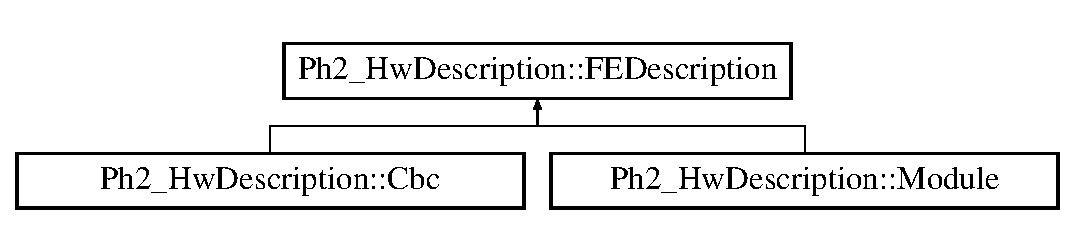
\includegraphics[height=2.000000cm]{class_ph2___hw_description_1_1_f_e_description}
\end{center}
\end{figure}
\subsection*{Public Member Functions}
\begin{DoxyCompactItemize}
\item 
\hyperlink{class_ph2___hw_description_1_1_f_e_description_a23be149c77c625424510e88adf3e95d4}{F\-E\-Description} (uint8\-\_\-t p\-Shelve\-Id, uint8\-\_\-t p\-Be\-Id, uint8\-\_\-t p\-F\-M\-C\-Id, uint8\-\_\-t p\-Fe\-Id, bool p\-Status=true)
\item 
\hyperlink{class_ph2___hw_description_1_1_f_e_description_acbcf750f0bf74a954eb50db7255e5c26}{F\-E\-Description} (uint8\-\_\-t p\-Be\-Id, uint8\-\_\-t p\-F\-M\-C\-Id, uint8\-\_\-t p\-Fe\-Id)
\item 
\hyperlink{class_ph2___hw_description_1_1_f_e_description_abc5f53987051c0d9746c97e1d993b143}{F\-E\-Description} ()
\item 
\hyperlink{class_ph2___hw_description_1_1_f_e_description_a1169ae7f8f71a37ff35b7c31f6452611}{F\-E\-Description} (const \hyperlink{class_ph2___hw_description_1_1_f_e_description}{F\-E\-Description} \&p\-Fe\-Desc)
\item 
virtual \hyperlink{class_ph2___hw_description_1_1_f_e_description_a6f055cd3fade537864dd7c3b34fede39}{$\sim$\-F\-E\-Description} ()
\item 
virtual uint8\-\_\-t \hyperlink{class_ph2___hw_description_1_1_f_e_description_a4e532c3b78e6a4a1b5f0022005898e25}{get\-Shelve\-Id} ()
\begin{DoxyCompactList}\small\item\em Get the Shelve I\-D. \end{DoxyCompactList}\item 
virtual uint8\-\_\-t \hyperlink{class_ph2___hw_description_1_1_f_e_description_a9077e5848363bf04b1c5860726879e79}{get\-Be\-Id} ()
\begin{DoxyCompactList}\small\item\em Get the Be I\-D. \end{DoxyCompactList}\item 
virtual uint8\-\_\-t \hyperlink{class_ph2___hw_description_1_1_f_e_description_a3bf79b7197bf731c85e9041f94ad4351}{get\-F\-M\-C\-Id} ()
\begin{DoxyCompactList}\small\item\em Get the F\-M\-C I\-D. \end{DoxyCompactList}\item 
virtual uint8\-\_\-t \hyperlink{class_ph2___hw_description_1_1_f_e_description_ab282dc785d2db2e8837b082d85fb9bb3}{get\-Fe\-Id} ()
\begin{DoxyCompactList}\small\item\em Get the F\-E I\-D. \end{DoxyCompactList}\item 
virtual bool \hyperlink{class_ph2___hw_description_1_1_f_e_description_a617ae77418832f97179026559685ea2d}{get\-Status} ()
\begin{DoxyCompactList}\small\item\em Get the Status. \end{DoxyCompactList}\item 
virtual uint8\-\_\-t \hyperlink{class_ph2___hw_description_1_1_f_e_description_ab207edf946f371bef6860fb6ce4deb65}{set\-Shelve\-Id} (uint8\-\_\-t p\-Shelve\-Id)
\begin{DoxyCompactList}\small\item\em Set the Shelve I\-D. \end{DoxyCompactList}\item 
virtual uint8\-\_\-t \hyperlink{class_ph2___hw_description_1_1_f_e_description_a13f1c20eb678b8e23d2590a8ff23d349}{set\-Be\-Id} (uint8\-\_\-t p\-Be\-Id)
\begin{DoxyCompactList}\small\item\em Set the Be I\-D. \end{DoxyCompactList}\item 
virtual uint8\-\_\-t \hyperlink{class_ph2___hw_description_1_1_f_e_description_af0c396a0475a508e8aca069bb5b3c577}{set\-F\-M\-C\-Id} (uint8\-\_\-t p\-F\-M\-C\-Id)
\begin{DoxyCompactList}\small\item\em Set the F\-M\-C I\-D. \end{DoxyCompactList}\item 
virtual uint8\-\_\-t \hyperlink{class_ph2___hw_description_1_1_f_e_description_a681786aea17ed86c40a3274783d5f6b5}{set\-Fe\-Id} (uint8\-\_\-t p\-Fe\-Id)
\begin{DoxyCompactList}\small\item\em Set the F\-E I\-D. \end{DoxyCompactList}\item 
virtual bool \hyperlink{class_ph2___hw_description_1_1_f_e_description_aa6e842d9be9aba79eccf5691ca6f7695}{set\-Status} (bool p\-Status)
\begin{DoxyCompactList}\small\item\em Set the status. \end{DoxyCompactList}\end{DoxyCompactItemize}
\subsection*{Data Fields}
\begin{DoxyCompactItemize}
\item 
uint8\-\_\-t \hyperlink{class_ph2___hw_description_1_1_f_e_description_a8a20ee1f2114b9a6da4483f5e0f8c625}{f\-Shelve\-Id}
\item 
uint8\-\_\-t \hyperlink{class_ph2___hw_description_1_1_f_e_description_ab279589109fe8a83ecd7cd6c631394b3}{f\-Be\-Id}
\item 
uint8\-\_\-t \hyperlink{class_ph2___hw_description_1_1_f_e_description_a7740e5ec6ae04ee47ac3081ff57e1946}{f\-F\-M\-C\-Id}
\item 
uint8\-\_\-t \hyperlink{class_ph2___hw_description_1_1_f_e_description_a3a1a3a8323484b1bfc1a4ab3d7a59a31}{f\-Fe\-Id}
\item 
bool \hyperlink{class_ph2___hw_description_1_1_f_e_description_a646f651eb15f15a519006eca502e3418}{f\-Status}
\end{DoxyCompactItemize}


\subsection{Detailed Description}
Describe all parameters common to all F\-E Components in the D\-A\-Q chain. 

\subsection{Constructor \& Destructor Documentation}
\hypertarget{class_ph2___hw_description_1_1_f_e_description_a23be149c77c625424510e88adf3e95d4}{\index{Ph2\-\_\-\-Hw\-Description\-::\-F\-E\-Description@{Ph2\-\_\-\-Hw\-Description\-::\-F\-E\-Description}!F\-E\-Description@{F\-E\-Description}}
\index{F\-E\-Description@{F\-E\-Description}!Ph2_HwDescription::FEDescription@{Ph2\-\_\-\-Hw\-Description\-::\-F\-E\-Description}}
\subsubsection[{F\-E\-Description}]{\setlength{\rightskip}{0pt plus 5cm}Ph2\-\_\-\-Hw\-Description\-::\-F\-E\-Description\-::\-F\-E\-Description (
\begin{DoxyParamCaption}
\item[{uint8\-\_\-t}]{p\-Shelve\-Id, }
\item[{uint8\-\_\-t}]{p\-Be\-Id, }
\item[{uint8\-\_\-t}]{p\-F\-M\-C\-Id, }
\item[{uint8\-\_\-t}]{p\-Fe\-Id, }
\item[{bool}]{p\-Status = {\ttfamily true}}
\end{DoxyParamCaption}
)}}\label{class_ph2___hw_description_1_1_f_e_description_a23be149c77c625424510e88adf3e95d4}
\hypertarget{class_ph2___hw_description_1_1_f_e_description_acbcf750f0bf74a954eb50db7255e5c26}{\index{Ph2\-\_\-\-Hw\-Description\-::\-F\-E\-Description@{Ph2\-\_\-\-Hw\-Description\-::\-F\-E\-Description}!F\-E\-Description@{F\-E\-Description}}
\index{F\-E\-Description@{F\-E\-Description}!Ph2_HwDescription::FEDescription@{Ph2\-\_\-\-Hw\-Description\-::\-F\-E\-Description}}
\subsubsection[{F\-E\-Description}]{\setlength{\rightskip}{0pt plus 5cm}Ph2\-\_\-\-Hw\-Description\-::\-F\-E\-Description\-::\-F\-E\-Description (
\begin{DoxyParamCaption}
\item[{uint8\-\_\-t}]{p\-Be\-Id, }
\item[{uint8\-\_\-t}]{p\-F\-M\-C\-Id, }
\item[{uint8\-\_\-t}]{p\-Fe\-Id}
\end{DoxyParamCaption}
)}}\label{class_ph2___hw_description_1_1_f_e_description_acbcf750f0bf74a954eb50db7255e5c26}
\hypertarget{class_ph2___hw_description_1_1_f_e_description_abc5f53987051c0d9746c97e1d993b143}{\index{Ph2\-\_\-\-Hw\-Description\-::\-F\-E\-Description@{Ph2\-\_\-\-Hw\-Description\-::\-F\-E\-Description}!F\-E\-Description@{F\-E\-Description}}
\index{F\-E\-Description@{F\-E\-Description}!Ph2_HwDescription::FEDescription@{Ph2\-\_\-\-Hw\-Description\-::\-F\-E\-Description}}
\subsubsection[{F\-E\-Description}]{\setlength{\rightskip}{0pt plus 5cm}Ph2\-\_\-\-Hw\-Description\-::\-F\-E\-Description\-::\-F\-E\-Description (
\begin{DoxyParamCaption}
{}
\end{DoxyParamCaption}
)}}\label{class_ph2___hw_description_1_1_f_e_description_abc5f53987051c0d9746c97e1d993b143}
\hypertarget{class_ph2___hw_description_1_1_f_e_description_a1169ae7f8f71a37ff35b7c31f6452611}{\index{Ph2\-\_\-\-Hw\-Description\-::\-F\-E\-Description@{Ph2\-\_\-\-Hw\-Description\-::\-F\-E\-Description}!F\-E\-Description@{F\-E\-Description}}
\index{F\-E\-Description@{F\-E\-Description}!Ph2_HwDescription::FEDescription@{Ph2\-\_\-\-Hw\-Description\-::\-F\-E\-Description}}
\subsubsection[{F\-E\-Description}]{\setlength{\rightskip}{0pt plus 5cm}Ph2\-\_\-\-Hw\-Description\-::\-F\-E\-Description\-::\-F\-E\-Description (
\begin{DoxyParamCaption}
\item[{const {\bf F\-E\-Description} \&}]{p\-Fe\-Desc}
\end{DoxyParamCaption}
)}}\label{class_ph2___hw_description_1_1_f_e_description_a1169ae7f8f71a37ff35b7c31f6452611}
\hypertarget{class_ph2___hw_description_1_1_f_e_description_a6f055cd3fade537864dd7c3b34fede39}{\index{Ph2\-\_\-\-Hw\-Description\-::\-F\-E\-Description@{Ph2\-\_\-\-Hw\-Description\-::\-F\-E\-Description}!$\sim$\-F\-E\-Description@{$\sim$\-F\-E\-Description}}
\index{$\sim$\-F\-E\-Description@{$\sim$\-F\-E\-Description}!Ph2_HwDescription::FEDescription@{Ph2\-\_\-\-Hw\-Description\-::\-F\-E\-Description}}
\subsubsection[{$\sim$\-F\-E\-Description}]{\setlength{\rightskip}{0pt plus 5cm}Ph2\-\_\-\-Hw\-Description\-::\-F\-E\-Description\-::$\sim$\-F\-E\-Description (
\begin{DoxyParamCaption}
{}
\end{DoxyParamCaption}
)\hspace{0.3cm}{\ttfamily [virtual]}}}\label{class_ph2___hw_description_1_1_f_e_description_a6f055cd3fade537864dd7c3b34fede39}


\subsection{Member Function Documentation}
\hypertarget{class_ph2___hw_description_1_1_f_e_description_a9077e5848363bf04b1c5860726879e79}{\index{Ph2\-\_\-\-Hw\-Description\-::\-F\-E\-Description@{Ph2\-\_\-\-Hw\-Description\-::\-F\-E\-Description}!get\-Be\-Id@{get\-Be\-Id}}
\index{get\-Be\-Id@{get\-Be\-Id}!Ph2_HwDescription::FEDescription@{Ph2\-\_\-\-Hw\-Description\-::\-F\-E\-Description}}
\subsubsection[{get\-Be\-Id}]{\setlength{\rightskip}{0pt plus 5cm}virtual uint8\-\_\-t Ph2\-\_\-\-Hw\-Description\-::\-F\-E\-Description\-::get\-Be\-Id (
\begin{DoxyParamCaption}
{}
\end{DoxyParamCaption}
)\hspace{0.3cm}{\ttfamily [inline]}, {\ttfamily [virtual]}}}\label{class_ph2___hw_description_1_1_f_e_description_a9077e5848363bf04b1c5860726879e79}


Get the Be I\-D. 

\begin{DoxyReturn}{Returns}
The Be I\-D 
\end{DoxyReturn}
\hypertarget{class_ph2___hw_description_1_1_f_e_description_ab282dc785d2db2e8837b082d85fb9bb3}{\index{Ph2\-\_\-\-Hw\-Description\-::\-F\-E\-Description@{Ph2\-\_\-\-Hw\-Description\-::\-F\-E\-Description}!get\-Fe\-Id@{get\-Fe\-Id}}
\index{get\-Fe\-Id@{get\-Fe\-Id}!Ph2_HwDescription::FEDescription@{Ph2\-\_\-\-Hw\-Description\-::\-F\-E\-Description}}
\subsubsection[{get\-Fe\-Id}]{\setlength{\rightskip}{0pt plus 5cm}virtual uint8\-\_\-t Ph2\-\_\-\-Hw\-Description\-::\-F\-E\-Description\-::get\-Fe\-Id (
\begin{DoxyParamCaption}
{}
\end{DoxyParamCaption}
)\hspace{0.3cm}{\ttfamily [inline]}, {\ttfamily [virtual]}}}\label{class_ph2___hw_description_1_1_f_e_description_ab282dc785d2db2e8837b082d85fb9bb3}


Get the F\-E I\-D. 

\begin{DoxyReturn}{Returns}
The F\-E I\-D 
\end{DoxyReturn}
\hypertarget{class_ph2___hw_description_1_1_f_e_description_a3bf79b7197bf731c85e9041f94ad4351}{\index{Ph2\-\_\-\-Hw\-Description\-::\-F\-E\-Description@{Ph2\-\_\-\-Hw\-Description\-::\-F\-E\-Description}!get\-F\-M\-C\-Id@{get\-F\-M\-C\-Id}}
\index{get\-F\-M\-C\-Id@{get\-F\-M\-C\-Id}!Ph2_HwDescription::FEDescription@{Ph2\-\_\-\-Hw\-Description\-::\-F\-E\-Description}}
\subsubsection[{get\-F\-M\-C\-Id}]{\setlength{\rightskip}{0pt plus 5cm}virtual uint8\-\_\-t Ph2\-\_\-\-Hw\-Description\-::\-F\-E\-Description\-::get\-F\-M\-C\-Id (
\begin{DoxyParamCaption}
{}
\end{DoxyParamCaption}
)\hspace{0.3cm}{\ttfamily [inline]}, {\ttfamily [virtual]}}}\label{class_ph2___hw_description_1_1_f_e_description_a3bf79b7197bf731c85e9041f94ad4351}


Get the F\-M\-C I\-D. 

\begin{DoxyReturn}{Returns}
The F\-M\-C I\-D 
\end{DoxyReturn}
\hypertarget{class_ph2___hw_description_1_1_f_e_description_a4e532c3b78e6a4a1b5f0022005898e25}{\index{Ph2\-\_\-\-Hw\-Description\-::\-F\-E\-Description@{Ph2\-\_\-\-Hw\-Description\-::\-F\-E\-Description}!get\-Shelve\-Id@{get\-Shelve\-Id}}
\index{get\-Shelve\-Id@{get\-Shelve\-Id}!Ph2_HwDescription::FEDescription@{Ph2\-\_\-\-Hw\-Description\-::\-F\-E\-Description}}
\subsubsection[{get\-Shelve\-Id}]{\setlength{\rightskip}{0pt plus 5cm}virtual uint8\-\_\-t Ph2\-\_\-\-Hw\-Description\-::\-F\-E\-Description\-::get\-Shelve\-Id (
\begin{DoxyParamCaption}
{}
\end{DoxyParamCaption}
)\hspace{0.3cm}{\ttfamily [inline]}, {\ttfamily [virtual]}}}\label{class_ph2___hw_description_1_1_f_e_description_a4e532c3b78e6a4a1b5f0022005898e25}


Get the Shelve I\-D. 

\begin{DoxyReturn}{Returns}
The Shelve I\-D 
\end{DoxyReturn}
\hypertarget{class_ph2___hw_description_1_1_f_e_description_a617ae77418832f97179026559685ea2d}{\index{Ph2\-\_\-\-Hw\-Description\-::\-F\-E\-Description@{Ph2\-\_\-\-Hw\-Description\-::\-F\-E\-Description}!get\-Status@{get\-Status}}
\index{get\-Status@{get\-Status}!Ph2_HwDescription::FEDescription@{Ph2\-\_\-\-Hw\-Description\-::\-F\-E\-Description}}
\subsubsection[{get\-Status}]{\setlength{\rightskip}{0pt plus 5cm}virtual bool Ph2\-\_\-\-Hw\-Description\-::\-F\-E\-Description\-::get\-Status (
\begin{DoxyParamCaption}
{}
\end{DoxyParamCaption}
)\hspace{0.3cm}{\ttfamily [inline]}, {\ttfamily [virtual]}}}\label{class_ph2___hw_description_1_1_f_e_description_a617ae77418832f97179026559685ea2d}


Get the Status. 

\begin{DoxyReturn}{Returns}
The Status 
\end{DoxyReturn}
\hypertarget{class_ph2___hw_description_1_1_f_e_description_a13f1c20eb678b8e23d2590a8ff23d349}{\index{Ph2\-\_\-\-Hw\-Description\-::\-F\-E\-Description@{Ph2\-\_\-\-Hw\-Description\-::\-F\-E\-Description}!set\-Be\-Id@{set\-Be\-Id}}
\index{set\-Be\-Id@{set\-Be\-Id}!Ph2_HwDescription::FEDescription@{Ph2\-\_\-\-Hw\-Description\-::\-F\-E\-Description}}
\subsubsection[{set\-Be\-Id}]{\setlength{\rightskip}{0pt plus 5cm}uint8\-\_\-t Ph2\-\_\-\-Hw\-Description\-::\-F\-E\-Description\-::set\-Be\-Id (
\begin{DoxyParamCaption}
\item[{uint8\-\_\-t}]{p\-Be\-Id}
\end{DoxyParamCaption}
)\hspace{0.3cm}{\ttfamily [virtual]}}}\label{class_ph2___hw_description_1_1_f_e_description_a13f1c20eb678b8e23d2590a8ff23d349}


Set the Be I\-D. 


\begin{DoxyParams}{Parameters}
{\em p\-Be\-Id} & \\
\hline
\end{DoxyParams}
\begin{DoxyReturn}{Returns}
the Be I\-D 
\end{DoxyReturn}
\hypertarget{class_ph2___hw_description_1_1_f_e_description_a681786aea17ed86c40a3274783d5f6b5}{\index{Ph2\-\_\-\-Hw\-Description\-::\-F\-E\-Description@{Ph2\-\_\-\-Hw\-Description\-::\-F\-E\-Description}!set\-Fe\-Id@{set\-Fe\-Id}}
\index{set\-Fe\-Id@{set\-Fe\-Id}!Ph2_HwDescription::FEDescription@{Ph2\-\_\-\-Hw\-Description\-::\-F\-E\-Description}}
\subsubsection[{set\-Fe\-Id}]{\setlength{\rightskip}{0pt plus 5cm}uint8\-\_\-t Ph2\-\_\-\-Hw\-Description\-::\-F\-E\-Description\-::set\-Fe\-Id (
\begin{DoxyParamCaption}
\item[{uint8\-\_\-t}]{p\-Fe\-Id}
\end{DoxyParamCaption}
)\hspace{0.3cm}{\ttfamily [virtual]}}}\label{class_ph2___hw_description_1_1_f_e_description_a681786aea17ed86c40a3274783d5f6b5}


Set the F\-E I\-D. 


\begin{DoxyParams}{Parameters}
{\em p\-Fe\-Id} & \\
\hline
\end{DoxyParams}
\begin{DoxyReturn}{Returns}
the Fe I\-D 
\end{DoxyReturn}
\hypertarget{class_ph2___hw_description_1_1_f_e_description_af0c396a0475a508e8aca069bb5b3c577}{\index{Ph2\-\_\-\-Hw\-Description\-::\-F\-E\-Description@{Ph2\-\_\-\-Hw\-Description\-::\-F\-E\-Description}!set\-F\-M\-C\-Id@{set\-F\-M\-C\-Id}}
\index{set\-F\-M\-C\-Id@{set\-F\-M\-C\-Id}!Ph2_HwDescription::FEDescription@{Ph2\-\_\-\-Hw\-Description\-::\-F\-E\-Description}}
\subsubsection[{set\-F\-M\-C\-Id}]{\setlength{\rightskip}{0pt plus 5cm}uint8\-\_\-t Ph2\-\_\-\-Hw\-Description\-::\-F\-E\-Description\-::set\-F\-M\-C\-Id (
\begin{DoxyParamCaption}
\item[{uint8\-\_\-t}]{p\-F\-M\-C\-Id}
\end{DoxyParamCaption}
)\hspace{0.3cm}{\ttfamily [virtual]}}}\label{class_ph2___hw_description_1_1_f_e_description_af0c396a0475a508e8aca069bb5b3c577}


Set the F\-M\-C I\-D. 


\begin{DoxyParams}{Parameters}
{\em p\-F\-M\-C\-Id} & \\
\hline
\end{DoxyParams}
\begin{DoxyReturn}{Returns}
the F\-M\-C I\-D 
\end{DoxyReturn}
\hypertarget{class_ph2___hw_description_1_1_f_e_description_ab207edf946f371bef6860fb6ce4deb65}{\index{Ph2\-\_\-\-Hw\-Description\-::\-F\-E\-Description@{Ph2\-\_\-\-Hw\-Description\-::\-F\-E\-Description}!set\-Shelve\-Id@{set\-Shelve\-Id}}
\index{set\-Shelve\-Id@{set\-Shelve\-Id}!Ph2_HwDescription::FEDescription@{Ph2\-\_\-\-Hw\-Description\-::\-F\-E\-Description}}
\subsubsection[{set\-Shelve\-Id}]{\setlength{\rightskip}{0pt plus 5cm}uint8\-\_\-t Ph2\-\_\-\-Hw\-Description\-::\-F\-E\-Description\-::set\-Shelve\-Id (
\begin{DoxyParamCaption}
\item[{uint8\-\_\-t}]{p\-Shelve\-Id}
\end{DoxyParamCaption}
)\hspace{0.3cm}{\ttfamily [virtual]}}}\label{class_ph2___hw_description_1_1_f_e_description_ab207edf946f371bef6860fb6ce4deb65}


Set the Shelve I\-D. 


\begin{DoxyParams}{Parameters}
{\em p\-Shelve\-Id} & \\
\hline
\end{DoxyParams}
\begin{DoxyReturn}{Returns}
the Shelve I\-D 
\end{DoxyReturn}
\hypertarget{class_ph2___hw_description_1_1_f_e_description_aa6e842d9be9aba79eccf5691ca6f7695}{\index{Ph2\-\_\-\-Hw\-Description\-::\-F\-E\-Description@{Ph2\-\_\-\-Hw\-Description\-::\-F\-E\-Description}!set\-Status@{set\-Status}}
\index{set\-Status@{set\-Status}!Ph2_HwDescription::FEDescription@{Ph2\-\_\-\-Hw\-Description\-::\-F\-E\-Description}}
\subsubsection[{set\-Status}]{\setlength{\rightskip}{0pt plus 5cm}bool Ph2\-\_\-\-Hw\-Description\-::\-F\-E\-Description\-::set\-Status (
\begin{DoxyParamCaption}
\item[{bool}]{p\-Status}
\end{DoxyParamCaption}
)\hspace{0.3cm}{\ttfamily [virtual]}}}\label{class_ph2___hw_description_1_1_f_e_description_aa6e842d9be9aba79eccf5691ca6f7695}


Set the status. 


\begin{DoxyParams}{Parameters}
{\em p\-Status} & \\
\hline
\end{DoxyParams}
\begin{DoxyReturn}{Returns}
the Status 
\end{DoxyReturn}


\subsection{Field Documentation}
\hypertarget{class_ph2___hw_description_1_1_f_e_description_ab279589109fe8a83ecd7cd6c631394b3}{\index{Ph2\-\_\-\-Hw\-Description\-::\-F\-E\-Description@{Ph2\-\_\-\-Hw\-Description\-::\-F\-E\-Description}!f\-Be\-Id@{f\-Be\-Id}}
\index{f\-Be\-Id@{f\-Be\-Id}!Ph2_HwDescription::FEDescription@{Ph2\-\_\-\-Hw\-Description\-::\-F\-E\-Description}}
\subsubsection[{f\-Be\-Id}]{\setlength{\rightskip}{0pt plus 5cm}uint8\-\_\-t Ph2\-\_\-\-Hw\-Description\-::\-F\-E\-Description\-::f\-Be\-Id}}\label{class_ph2___hw_description_1_1_f_e_description_ab279589109fe8a83ecd7cd6c631394b3}
\hypertarget{class_ph2___hw_description_1_1_f_e_description_a3a1a3a8323484b1bfc1a4ab3d7a59a31}{\index{Ph2\-\_\-\-Hw\-Description\-::\-F\-E\-Description@{Ph2\-\_\-\-Hw\-Description\-::\-F\-E\-Description}!f\-Fe\-Id@{f\-Fe\-Id}}
\index{f\-Fe\-Id@{f\-Fe\-Id}!Ph2_HwDescription::FEDescription@{Ph2\-\_\-\-Hw\-Description\-::\-F\-E\-Description}}
\subsubsection[{f\-Fe\-Id}]{\setlength{\rightskip}{0pt plus 5cm}uint8\-\_\-t Ph2\-\_\-\-Hw\-Description\-::\-F\-E\-Description\-::f\-Fe\-Id}}\label{class_ph2___hw_description_1_1_f_e_description_a3a1a3a8323484b1bfc1a4ab3d7a59a31}
\hypertarget{class_ph2___hw_description_1_1_f_e_description_a7740e5ec6ae04ee47ac3081ff57e1946}{\index{Ph2\-\_\-\-Hw\-Description\-::\-F\-E\-Description@{Ph2\-\_\-\-Hw\-Description\-::\-F\-E\-Description}!f\-F\-M\-C\-Id@{f\-F\-M\-C\-Id}}
\index{f\-F\-M\-C\-Id@{f\-F\-M\-C\-Id}!Ph2_HwDescription::FEDescription@{Ph2\-\_\-\-Hw\-Description\-::\-F\-E\-Description}}
\subsubsection[{f\-F\-M\-C\-Id}]{\setlength{\rightskip}{0pt plus 5cm}uint8\-\_\-t Ph2\-\_\-\-Hw\-Description\-::\-F\-E\-Description\-::f\-F\-M\-C\-Id}}\label{class_ph2___hw_description_1_1_f_e_description_a7740e5ec6ae04ee47ac3081ff57e1946}
\hypertarget{class_ph2___hw_description_1_1_f_e_description_a8a20ee1f2114b9a6da4483f5e0f8c625}{\index{Ph2\-\_\-\-Hw\-Description\-::\-F\-E\-Description@{Ph2\-\_\-\-Hw\-Description\-::\-F\-E\-Description}!f\-Shelve\-Id@{f\-Shelve\-Id}}
\index{f\-Shelve\-Id@{f\-Shelve\-Id}!Ph2_HwDescription::FEDescription@{Ph2\-\_\-\-Hw\-Description\-::\-F\-E\-Description}}
\subsubsection[{f\-Shelve\-Id}]{\setlength{\rightskip}{0pt plus 5cm}uint8\-\_\-t Ph2\-\_\-\-Hw\-Description\-::\-F\-E\-Description\-::f\-Shelve\-Id}}\label{class_ph2___hw_description_1_1_f_e_description_a8a20ee1f2114b9a6da4483f5e0f8c625}
\hypertarget{class_ph2___hw_description_1_1_f_e_description_a646f651eb15f15a519006eca502e3418}{\index{Ph2\-\_\-\-Hw\-Description\-::\-F\-E\-Description@{Ph2\-\_\-\-Hw\-Description\-::\-F\-E\-Description}!f\-Status@{f\-Status}}
\index{f\-Status@{f\-Status}!Ph2_HwDescription::FEDescription@{Ph2\-\_\-\-Hw\-Description\-::\-F\-E\-Description}}
\subsubsection[{f\-Status}]{\setlength{\rightskip}{0pt plus 5cm}bool Ph2\-\_\-\-Hw\-Description\-::\-F\-E\-Description\-::f\-Status}}\label{class_ph2___hw_description_1_1_f_e_description_a646f651eb15f15a519006eca502e3418}


The documentation for this class was generated from the following files\-:\begin{DoxyCompactItemize}
\item 
H\-W\-Description/\hyperlink{_f_e_description_8h}{F\-E\-Description.\-h}\item 
H\-W\-Description/\hyperlink{_f_e_description_8cc}{F\-E\-Description.\-cc}\end{DoxyCompactItemize}

\hypertarget{class_ph2___hw_description_1_1_glib}{\section{Ph2\-\_\-\-Hw\-Description\-:\-:Glib Class Reference}
\label{class_ph2___hw_description_1_1_glib}\index{Ph2\-\_\-\-Hw\-Description\-::\-Glib@{Ph2\-\_\-\-Hw\-Description\-::\-Glib}}
}


{\ttfamily \#include $<$Glib.\-h$>$}

\subsection*{Public Member Functions}
\begin{DoxyCompactItemize}
\item 
\hyperlink{class_ph2___hw_description_1_1_glib_ac63dbf3825526283c7cefc5e217e1c38}{Glib} (uint8\-\_\-t p\-Shelve\-Id, uint8\-\_\-t p\-Be\-Id, uint8\-\_\-t p\-N\-Fe, std\-::string filename=\hyperlink{_glib_8h_a3b2796757992a47db4ed9462093d6fe3}{default\-\_\-glib\-\_\-file})
\item 
\hyperlink{class_ph2___hw_description_1_1_glib_a05a22fe40ace0d74f5493cbded54bd99}{Glib} (uint8\-\_\-t p\-Shelve\-Id, uint8\-\_\-t p\-Be\-Id, uint8\-\_\-t p\-N\-Fe, bool p\-Ext\-Trg, bool p\-Fake\-Data=false, std\-::string filename=\char`\"{}default\-\_\-glib\-\_\-file\char`\"{})
\item 
\hyperlink{class_ph2___hw_description_1_1_glib_a2d9eece9012cdc452f43895852693329}{Glib} ()
\item 
\hyperlink{class_ph2___hw_description_1_1_glib_a2fa668cf8b827199d63be060616a70cd}{$\sim$\-Glib} ()
\item 
uint8\-\_\-t \hyperlink{class_ph2___hw_description_1_1_glib_a2675c993dad690792592ba3e30036bab}{get\-N\-Fe} ()
\item 
uint8\-\_\-t \hyperlink{class_ph2___hw_description_1_1_glib_a27f5e85e68f25e56d1096306e3f70188}{get\-Be\-Id} ()
\item 
uint8\-\_\-t \hyperlink{class_ph2___hw_description_1_1_glib_ac3130c4a08d624c6d89fc66474efd6d8}{get\-Shelve\-Id} ()
\item 
uint8\-\_\-t \hyperlink{class_ph2___hw_description_1_1_glib_ade845c9d6a9fcaaac1766cf89592fb97}{get\-Reg} (std\-::string p\-Reg)
\item 
void \hyperlink{class_ph2___hw_description_1_1_glib_a017ab68372401fe244b912a5297b0c33}{set\-Reg} (std\-::string p\-Reg, uint8\-\_\-t pset\-Value)
\item 
void \hyperlink{class_ph2___hw_description_1_1_glib_a1bbf1eb3a5d4efca9801d2eaca6f33f7}{add\-Module} (\hyperlink{class_ph2___hw_description_1_1_module}{Module} \&p\-Module)
\item 
bool \hyperlink{class_ph2___hw_description_1_1_glib_a64d98cba80674893dff1a91c69b0f34e}{remove\-Module} (uint8\-\_\-t p\-Module\-Id)
\item 
\hyperlink{class_ph2___hw_description_1_1_module}{Module} $\ast$ \hyperlink{class_ph2___hw_description_1_1_glib_a41e024e9138acdcb856c0f5c8c43be43}{get\-Module} (uint8\-\_\-t p\-Module\-Id)
\item 
std\-::map$<$ std\-::string, uint8\-\_\-t $>$ \hyperlink{class_ph2___hw_description_1_1_glib_a971d4ea45771b8f93ca81bc794613262}{get\-Glib\-Reg\-Map} ()
\end{DoxyCompactItemize}
\subsection*{Protected Attributes}
\begin{DoxyCompactItemize}
\item 
uint8\-\_\-t \hyperlink{class_ph2___hw_description_1_1_glib_abcaa5b1cb716d3aa814688dd5691a421}{f\-Shelve\-Id}
\item 
uint8\-\_\-t \hyperlink{class_ph2___hw_description_1_1_glib_ac89e9a9eee11e41f901e90c619e50bfc}{f\-Be\-Id}
\item 
std\-::vector$<$ \hyperlink{class_ph2___hw_description_1_1_module}{Module} $>$ \hyperlink{class_ph2___hw_description_1_1_glib_a97b6535900b4fa8eef81c7e15a01cda4}{f\-Module\-Vector}
\item 
\hyperlink{namespace_ph2___hw_description_afc0e75a92548c3406e89bf39ca4c9bfb}{Glib\-Reg\-Map} \hyperlink{class_ph2___hw_description_1_1_glib_a1a0c6dba5a24c615e8609b03012a8970}{f\-Reg\-Map}
\end{DoxyCompactItemize}
\subsection*{Private Member Functions}
\begin{DoxyCompactItemize}
\item 
void \hyperlink{class_ph2___hw_description_1_1_glib_a2eb8576c349ced2ac44904179294bd42}{load\-Config\-File} (std\-::string filename)
\end{DoxyCompactItemize}


\subsection{Constructor \& Destructor Documentation}
\hypertarget{class_ph2___hw_description_1_1_glib_ac63dbf3825526283c7cefc5e217e1c38}{\index{Ph2\-\_\-\-Hw\-Description\-::\-Glib@{Ph2\-\_\-\-Hw\-Description\-::\-Glib}!Glib@{Glib}}
\index{Glib@{Glib}!Ph2_HwDescription::Glib@{Ph2\-\_\-\-Hw\-Description\-::\-Glib}}
\subsubsection[{Glib}]{\setlength{\rightskip}{0pt plus 5cm}Ph2\-\_\-\-Hw\-Description\-::\-Glib\-::\-Glib (
\begin{DoxyParamCaption}
\item[{uint8\-\_\-t}]{p\-Shelve\-Id, }
\item[{uint8\-\_\-t}]{p\-Be\-Id, }
\item[{uint8\-\_\-t}]{p\-N\-Fe, }
\item[{std\-::string}]{filename = {\ttfamily {\bf default\-\_\-glib\-\_\-file}}}
\end{DoxyParamCaption}
)}}\label{class_ph2___hw_description_1_1_glib_ac63dbf3825526283c7cefc5e217e1c38}
\hypertarget{class_ph2___hw_description_1_1_glib_a05a22fe40ace0d74f5493cbded54bd99}{\index{Ph2\-\_\-\-Hw\-Description\-::\-Glib@{Ph2\-\_\-\-Hw\-Description\-::\-Glib}!Glib@{Glib}}
\index{Glib@{Glib}!Ph2_HwDescription::Glib@{Ph2\-\_\-\-Hw\-Description\-::\-Glib}}
\subsubsection[{Glib}]{\setlength{\rightskip}{0pt plus 5cm}Ph2\-\_\-\-Hw\-Description\-::\-Glib\-::\-Glib (
\begin{DoxyParamCaption}
\item[{uint8\-\_\-t}]{p\-Shelve\-Id, }
\item[{uint8\-\_\-t}]{p\-Be\-Id, }
\item[{uint8\-\_\-t}]{p\-N\-Fe, }
\item[{bool}]{p\-Ext\-Trg, }
\item[{bool}]{p\-Fake\-Data = {\ttfamily false}, }
\item[{std\-::string}]{filename = {\ttfamily \char`\"{}default\-\_\-glib\-\_\-file\char`\"{}}}
\end{DoxyParamCaption}
)}}\label{class_ph2___hw_description_1_1_glib_a05a22fe40ace0d74f5493cbded54bd99}
\hypertarget{class_ph2___hw_description_1_1_glib_a2d9eece9012cdc452f43895852693329}{\index{Ph2\-\_\-\-Hw\-Description\-::\-Glib@{Ph2\-\_\-\-Hw\-Description\-::\-Glib}!Glib@{Glib}}
\index{Glib@{Glib}!Ph2_HwDescription::Glib@{Ph2\-\_\-\-Hw\-Description\-::\-Glib}}
\subsubsection[{Glib}]{\setlength{\rightskip}{0pt plus 5cm}Ph2\-\_\-\-Hw\-Description\-::\-Glib\-::\-Glib (
\begin{DoxyParamCaption}
{}
\end{DoxyParamCaption}
)}}\label{class_ph2___hw_description_1_1_glib_a2d9eece9012cdc452f43895852693329}
\hypertarget{class_ph2___hw_description_1_1_glib_a2fa668cf8b827199d63be060616a70cd}{\index{Ph2\-\_\-\-Hw\-Description\-::\-Glib@{Ph2\-\_\-\-Hw\-Description\-::\-Glib}!$\sim$\-Glib@{$\sim$\-Glib}}
\index{$\sim$\-Glib@{$\sim$\-Glib}!Ph2_HwDescription::Glib@{Ph2\-\_\-\-Hw\-Description\-::\-Glib}}
\subsubsection[{$\sim$\-Glib}]{\setlength{\rightskip}{0pt plus 5cm}Ph2\-\_\-\-Hw\-Description\-::\-Glib\-::$\sim$\-Glib (
\begin{DoxyParamCaption}
{}
\end{DoxyParamCaption}
)\hspace{0.3cm}{\ttfamily [inline]}}}\label{class_ph2___hw_description_1_1_glib_a2fa668cf8b827199d63be060616a70cd}


\subsection{Member Function Documentation}
\hypertarget{class_ph2___hw_description_1_1_glib_a1bbf1eb3a5d4efca9801d2eaca6f33f7}{\index{Ph2\-\_\-\-Hw\-Description\-::\-Glib@{Ph2\-\_\-\-Hw\-Description\-::\-Glib}!add\-Module@{add\-Module}}
\index{add\-Module@{add\-Module}!Ph2_HwDescription::Glib@{Ph2\-\_\-\-Hw\-Description\-::\-Glib}}
\subsubsection[{add\-Module}]{\setlength{\rightskip}{0pt plus 5cm}void Ph2\-\_\-\-Hw\-Description\-::\-Glib\-::add\-Module (
\begin{DoxyParamCaption}
\item[{{\bf Module} \&}]{p\-Module}
\end{DoxyParamCaption}
)}}\label{class_ph2___hw_description_1_1_glib_a1bbf1eb3a5d4efca9801d2eaca6f33f7}
\hypertarget{class_ph2___hw_description_1_1_glib_a27f5e85e68f25e56d1096306e3f70188}{\index{Ph2\-\_\-\-Hw\-Description\-::\-Glib@{Ph2\-\_\-\-Hw\-Description\-::\-Glib}!get\-Be\-Id@{get\-Be\-Id}}
\index{get\-Be\-Id@{get\-Be\-Id}!Ph2_HwDescription::Glib@{Ph2\-\_\-\-Hw\-Description\-::\-Glib}}
\subsubsection[{get\-Be\-Id}]{\setlength{\rightskip}{0pt plus 5cm}uint8\-\_\-t Ph2\-\_\-\-Hw\-Description\-::\-Glib\-::get\-Be\-Id (
\begin{DoxyParamCaption}
{}
\end{DoxyParamCaption}
)\hspace{0.3cm}{\ttfamily [inline]}}}\label{class_ph2___hw_description_1_1_glib_a27f5e85e68f25e56d1096306e3f70188}
\hypertarget{class_ph2___hw_description_1_1_glib_a971d4ea45771b8f93ca81bc794613262}{\index{Ph2\-\_\-\-Hw\-Description\-::\-Glib@{Ph2\-\_\-\-Hw\-Description\-::\-Glib}!get\-Glib\-Reg\-Map@{get\-Glib\-Reg\-Map}}
\index{get\-Glib\-Reg\-Map@{get\-Glib\-Reg\-Map}!Ph2_HwDescription::Glib@{Ph2\-\_\-\-Hw\-Description\-::\-Glib}}
\subsubsection[{get\-Glib\-Reg\-Map}]{\setlength{\rightskip}{0pt plus 5cm}std\-::map$<$ std\-::string, uint8\-\_\-t $>$ Ph2\-\_\-\-Hw\-Description\-::\-Glib\-::get\-Glib\-Reg\-Map (
\begin{DoxyParamCaption}
{}
\end{DoxyParamCaption}
)\hspace{0.3cm}{\ttfamily [inline]}}}\label{class_ph2___hw_description_1_1_glib_a971d4ea45771b8f93ca81bc794613262}
\hypertarget{class_ph2___hw_description_1_1_glib_a41e024e9138acdcb856c0f5c8c43be43}{\index{Ph2\-\_\-\-Hw\-Description\-::\-Glib@{Ph2\-\_\-\-Hw\-Description\-::\-Glib}!get\-Module@{get\-Module}}
\index{get\-Module@{get\-Module}!Ph2_HwDescription::Glib@{Ph2\-\_\-\-Hw\-Description\-::\-Glib}}
\subsubsection[{get\-Module}]{\setlength{\rightskip}{0pt plus 5cm}{\bf Module} $\ast$ Ph2\-\_\-\-Hw\-Description\-::\-Glib\-::get\-Module (
\begin{DoxyParamCaption}
\item[{uint8\-\_\-t}]{p\-Module\-Id}
\end{DoxyParamCaption}
)}}\label{class_ph2___hw_description_1_1_glib_a41e024e9138acdcb856c0f5c8c43be43}
\hypertarget{class_ph2___hw_description_1_1_glib_a2675c993dad690792592ba3e30036bab}{\index{Ph2\-\_\-\-Hw\-Description\-::\-Glib@{Ph2\-\_\-\-Hw\-Description\-::\-Glib}!get\-N\-Fe@{get\-N\-Fe}}
\index{get\-N\-Fe@{get\-N\-Fe}!Ph2_HwDescription::Glib@{Ph2\-\_\-\-Hw\-Description\-::\-Glib}}
\subsubsection[{get\-N\-Fe}]{\setlength{\rightskip}{0pt plus 5cm}uint8\-\_\-t Ph2\-\_\-\-Hw\-Description\-::\-Glib\-::get\-N\-Fe (
\begin{DoxyParamCaption}
{}
\end{DoxyParamCaption}
)\hspace{0.3cm}{\ttfamily [inline]}}}\label{class_ph2___hw_description_1_1_glib_a2675c993dad690792592ba3e30036bab}
\hypertarget{class_ph2___hw_description_1_1_glib_ade845c9d6a9fcaaac1766cf89592fb97}{\index{Ph2\-\_\-\-Hw\-Description\-::\-Glib@{Ph2\-\_\-\-Hw\-Description\-::\-Glib}!get\-Reg@{get\-Reg}}
\index{get\-Reg@{get\-Reg}!Ph2_HwDescription::Glib@{Ph2\-\_\-\-Hw\-Description\-::\-Glib}}
\subsubsection[{get\-Reg}]{\setlength{\rightskip}{0pt plus 5cm}uint8\-\_\-t Ph2\-\_\-\-Hw\-Description\-::\-Glib\-::get\-Reg (
\begin{DoxyParamCaption}
\item[{std\-::string}]{p\-Reg}
\end{DoxyParamCaption}
)}}\label{class_ph2___hw_description_1_1_glib_ade845c9d6a9fcaaac1766cf89592fb97}
\hypertarget{class_ph2___hw_description_1_1_glib_ac3130c4a08d624c6d89fc66474efd6d8}{\index{Ph2\-\_\-\-Hw\-Description\-::\-Glib@{Ph2\-\_\-\-Hw\-Description\-::\-Glib}!get\-Shelve\-Id@{get\-Shelve\-Id}}
\index{get\-Shelve\-Id@{get\-Shelve\-Id}!Ph2_HwDescription::Glib@{Ph2\-\_\-\-Hw\-Description\-::\-Glib}}
\subsubsection[{get\-Shelve\-Id}]{\setlength{\rightskip}{0pt plus 5cm}uint8\-\_\-t Ph2\-\_\-\-Hw\-Description\-::\-Glib\-::get\-Shelve\-Id (
\begin{DoxyParamCaption}
{}
\end{DoxyParamCaption}
)\hspace{0.3cm}{\ttfamily [inline]}}}\label{class_ph2___hw_description_1_1_glib_ac3130c4a08d624c6d89fc66474efd6d8}
\hypertarget{class_ph2___hw_description_1_1_glib_a2eb8576c349ced2ac44904179294bd42}{\index{Ph2\-\_\-\-Hw\-Description\-::\-Glib@{Ph2\-\_\-\-Hw\-Description\-::\-Glib}!load\-Config\-File@{load\-Config\-File}}
\index{load\-Config\-File@{load\-Config\-File}!Ph2_HwDescription::Glib@{Ph2\-\_\-\-Hw\-Description\-::\-Glib}}
\subsubsection[{load\-Config\-File}]{\setlength{\rightskip}{0pt plus 5cm}void Ph2\-\_\-\-Hw\-Description\-::\-Glib\-::load\-Config\-File (
\begin{DoxyParamCaption}
\item[{std\-::string}]{filename}
\end{DoxyParamCaption}
)\hspace{0.3cm}{\ttfamily [private]}}}\label{class_ph2___hw_description_1_1_glib_a2eb8576c349ced2ac44904179294bd42}
\hypertarget{class_ph2___hw_description_1_1_glib_a64d98cba80674893dff1a91c69b0f34e}{\index{Ph2\-\_\-\-Hw\-Description\-::\-Glib@{Ph2\-\_\-\-Hw\-Description\-::\-Glib}!remove\-Module@{remove\-Module}}
\index{remove\-Module@{remove\-Module}!Ph2_HwDescription::Glib@{Ph2\-\_\-\-Hw\-Description\-::\-Glib}}
\subsubsection[{remove\-Module}]{\setlength{\rightskip}{0pt plus 5cm}bool Ph2\-\_\-\-Hw\-Description\-::\-Glib\-::remove\-Module (
\begin{DoxyParamCaption}
\item[{uint8\-\_\-t}]{p\-Module\-Id}
\end{DoxyParamCaption}
)}}\label{class_ph2___hw_description_1_1_glib_a64d98cba80674893dff1a91c69b0f34e}
\hypertarget{class_ph2___hw_description_1_1_glib_a017ab68372401fe244b912a5297b0c33}{\index{Ph2\-\_\-\-Hw\-Description\-::\-Glib@{Ph2\-\_\-\-Hw\-Description\-::\-Glib}!set\-Reg@{set\-Reg}}
\index{set\-Reg@{set\-Reg}!Ph2_HwDescription::Glib@{Ph2\-\_\-\-Hw\-Description\-::\-Glib}}
\subsubsection[{set\-Reg}]{\setlength{\rightskip}{0pt plus 5cm}void Ph2\-\_\-\-Hw\-Description\-::\-Glib\-::set\-Reg (
\begin{DoxyParamCaption}
\item[{std\-::string}]{p\-Reg, }
\item[{uint8\-\_\-t}]{pset\-Value}
\end{DoxyParamCaption}
)}}\label{class_ph2___hw_description_1_1_glib_a017ab68372401fe244b912a5297b0c33}


\subsection{Field Documentation}
\hypertarget{class_ph2___hw_description_1_1_glib_ac89e9a9eee11e41f901e90c619e50bfc}{\index{Ph2\-\_\-\-Hw\-Description\-::\-Glib@{Ph2\-\_\-\-Hw\-Description\-::\-Glib}!f\-Be\-Id@{f\-Be\-Id}}
\index{f\-Be\-Id@{f\-Be\-Id}!Ph2_HwDescription::Glib@{Ph2\-\_\-\-Hw\-Description\-::\-Glib}}
\subsubsection[{f\-Be\-Id}]{\setlength{\rightskip}{0pt plus 5cm}uint8\-\_\-t Ph2\-\_\-\-Hw\-Description\-::\-Glib\-::f\-Be\-Id\hspace{0.3cm}{\ttfamily [protected]}}}\label{class_ph2___hw_description_1_1_glib_ac89e9a9eee11e41f901e90c619e50bfc}
\hypertarget{class_ph2___hw_description_1_1_glib_a97b6535900b4fa8eef81c7e15a01cda4}{\index{Ph2\-\_\-\-Hw\-Description\-::\-Glib@{Ph2\-\_\-\-Hw\-Description\-::\-Glib}!f\-Module\-Vector@{f\-Module\-Vector}}
\index{f\-Module\-Vector@{f\-Module\-Vector}!Ph2_HwDescription::Glib@{Ph2\-\_\-\-Hw\-Description\-::\-Glib}}
\subsubsection[{f\-Module\-Vector}]{\setlength{\rightskip}{0pt plus 5cm}std\-::vector$<$ {\bf Module} $>$ Ph2\-\_\-\-Hw\-Description\-::\-Glib\-::f\-Module\-Vector\hspace{0.3cm}{\ttfamily [protected]}}}\label{class_ph2___hw_description_1_1_glib_a97b6535900b4fa8eef81c7e15a01cda4}
\hypertarget{class_ph2___hw_description_1_1_glib_a1a0c6dba5a24c615e8609b03012a8970}{\index{Ph2\-\_\-\-Hw\-Description\-::\-Glib@{Ph2\-\_\-\-Hw\-Description\-::\-Glib}!f\-Reg\-Map@{f\-Reg\-Map}}
\index{f\-Reg\-Map@{f\-Reg\-Map}!Ph2_HwDescription::Glib@{Ph2\-\_\-\-Hw\-Description\-::\-Glib}}
\subsubsection[{f\-Reg\-Map}]{\setlength{\rightskip}{0pt plus 5cm}{\bf Glib\-Reg\-Map} Ph2\-\_\-\-Hw\-Description\-::\-Glib\-::f\-Reg\-Map\hspace{0.3cm}{\ttfamily [protected]}}}\label{class_ph2___hw_description_1_1_glib_a1a0c6dba5a24c615e8609b03012a8970}
\hypertarget{class_ph2___hw_description_1_1_glib_abcaa5b1cb716d3aa814688dd5691a421}{\index{Ph2\-\_\-\-Hw\-Description\-::\-Glib@{Ph2\-\_\-\-Hw\-Description\-::\-Glib}!f\-Shelve\-Id@{f\-Shelve\-Id}}
\index{f\-Shelve\-Id@{f\-Shelve\-Id}!Ph2_HwDescription::Glib@{Ph2\-\_\-\-Hw\-Description\-::\-Glib}}
\subsubsection[{f\-Shelve\-Id}]{\setlength{\rightskip}{0pt plus 5cm}uint8\-\_\-t Ph2\-\_\-\-Hw\-Description\-::\-Glib\-::f\-Shelve\-Id\hspace{0.3cm}{\ttfamily [protected]}}}\label{class_ph2___hw_description_1_1_glib_abcaa5b1cb716d3aa814688dd5691a421}


The documentation for this class was generated from the following files\-:\begin{DoxyCompactItemize}
\item 
H\-W\-Description/\hyperlink{_glib_8h}{Glib.\-h}\item 
H\-W\-Description/\hyperlink{_glib_8cc}{Glib.\-cc}\end{DoxyCompactItemize}

\hypertarget{class_ph2___hw_interface_1_1_glib_interface}{\section{Ph2\-\_\-\-Hw\-Interface\-:\-:Glib\-Interface Class Reference}
\label{class_ph2___hw_interface_1_1_glib_interface}\index{Ph2\-\_\-\-Hw\-Interface\-::\-Glib\-Interface@{Ph2\-\_\-\-Hw\-Interface\-::\-Glib\-Interface}}
}


Permit r/w given registers in the Glib you specify.  




{\ttfamily \#include $<$G\-L\-I\-B\-Interface.\-h$>$}

Inheritance diagram for Ph2\-\_\-\-Hw\-Interface\-:\-:Glib\-Interface\-:\begin{figure}[H]
\begin{center}
\leavevmode
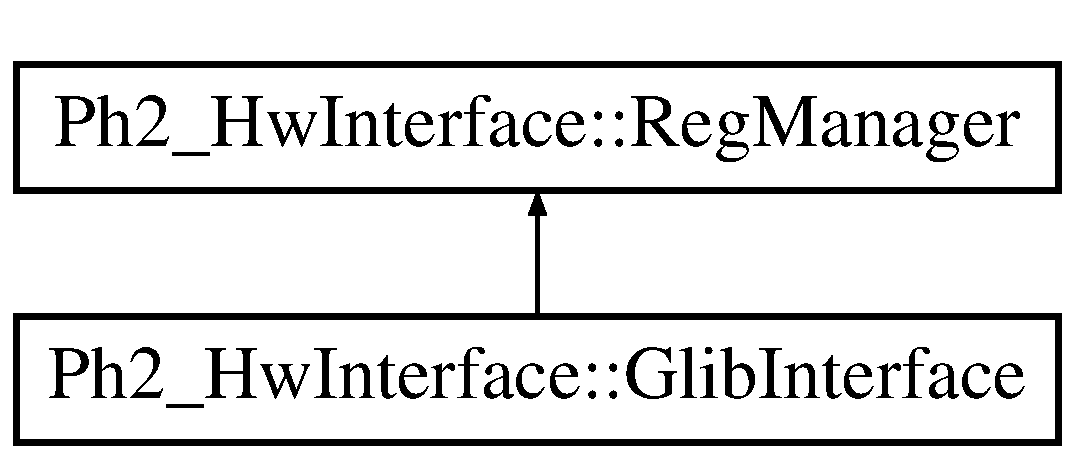
\includegraphics[height=2.000000cm]{class_ph2___hw_interface_1_1_glib_interface}
\end{center}
\end{figure}
\subsection*{Public Member Functions}
\begin{DoxyCompactItemize}
\item 
\hyperlink{class_ph2___hw_interface_1_1_glib_interface_a4aebde48748debad7e261c654c2c6fd8}{Glib\-Interface} (const char $\ast$pu\-Hal\-Config\-File\-Name)
\begin{DoxyCompactList}\small\item\em Constructor of the \hyperlink{class_ph2___hw_interface_1_1_glib_interface}{Glib\-Interface} class. \end{DoxyCompactList}\item 
\hyperlink{class_ph2___hw_interface_1_1_glib_interface_a1182c81cb29bca33b23a2c9f662df2ed}{$\sim$\-Glib\-Interface} ()
\begin{DoxyCompactList}\small\item\em Destructor of the \hyperlink{class_ph2___hw_interface_1_1_glib_interface}{Glib\-Interface} class. \end{DoxyCompactList}\item 
void \hyperlink{class_ph2___hw_interface_1_1_glib_interface_a51dd2e5a8128fd01a41c4d6b204df948}{get\-Board\-Info} (\hyperlink{class_ph2___hw_description_1_1_glib}{Glib} \&p\-Glib)
\begin{DoxyCompactList}\small\item\em Get the board infos. \end{DoxyCompactList}\item 
void \hyperlink{class_ph2___hw_interface_1_1_glib_interface_ad53d40d7cfea163bd3dcd04e233a02e3}{Select\-F\-E\-Id} (\hyperlink{class_ph2___hw_description_1_1_glib}{Glib} \&p\-Glib)
\begin{DoxyCompactList}\small\item\em Detect the right F\-E Id to write the right registers. \end{DoxyCompactList}\item 
void \hyperlink{class_ph2___hw_interface_1_1_glib_interface_aad68569190ea9b318b5be1abae4fd23f}{Configure\-Glib} (\hyperlink{class_ph2___hw_description_1_1_glib}{Glib} \&p\-Glib)
\begin{DoxyCompactList}\small\item\em Configure the Glib with its Config File. \end{DoxyCompactList}\item 
void \hyperlink{class_ph2___hw_interface_1_1_glib_interface_a0706eb396293fe5c8c717c5d0ab82165}{Start} (\hyperlink{class_ph2___hw_description_1_1_glib}{Glib} \&p\-Glib)
\begin{DoxyCompactList}\small\item\em Start a D\-A\-Q. \end{DoxyCompactList}\item 
void \hyperlink{class_ph2___hw_interface_1_1_glib_interface_a3073d292371ab4e602900f4276a43b6c}{Stop} (\hyperlink{class_ph2___hw_description_1_1_glib}{Glib} \&p\-Glib, uint32\-\_\-t p\-Nth\-Acq)
\begin{DoxyCompactList}\small\item\em Stop a D\-A\-Q. \end{DoxyCompactList}\item 
void \hyperlink{class_ph2___hw_interface_1_1_glib_interface_a1db7815b60c3e3637b23bfa27bab9692}{Pause} (\hyperlink{class_ph2___hw_description_1_1_glib}{Glib} \&p\-Glib)
\begin{DoxyCompactList}\small\item\em Pause a D\-A\-Q. \end{DoxyCompactList}\item 
void \hyperlink{class_ph2___hw_interface_1_1_glib_interface_a4d6568c22d8e3777ee909db37b3b01d6}{Unpause} (\hyperlink{class_ph2___hw_description_1_1_glib}{Glib} \&p\-Glib)
\begin{DoxyCompactList}\small\item\em Unpause a D\-A\-Q. \end{DoxyCompactList}\item 
void \hyperlink{class_ph2___hw_interface_1_1_glib_interface_ad3f91f03b0214987f4a9e8b63ff99dca}{Read\-Data} (\hyperlink{class_ph2___hw_description_1_1_glib}{Glib} \&p\-Glib, uint32\-\_\-t p\-Nth\-Acq, bool p\-Break\-Trigger)
\begin{DoxyCompactList}\small\item\em Read data from D\-A\-Q. \end{DoxyCompactList}\item 
void \hyperlink{class_ph2___hw_interface_1_1_glib_interface_a116aca1863dda40c52ca63259cd073b9}{Run} (\hyperlink{class_ph2___hw_description_1_1_glib}{Glib} \&p\-Glib)
\begin{DoxyCompactList}\small\item\em Run a D\-A\-Q. \end{DoxyCompactList}\item 
void \hyperlink{class_ph2___hw_interface_1_1_glib_interface_afeda624fe12657712e9f10cd60603d8a}{Update\-Glib\-Write} (\hyperlink{class_ph2___hw_description_1_1_glib}{Glib} \&p\-Glib, const std\-::string \&p\-Reg\-Node, const uint32\-\_\-t \&p\-Val)
\begin{DoxyCompactList}\small\item\em Update both Glib register and Config File. \end{DoxyCompactList}\item 
void \hyperlink{class_ph2___hw_interface_1_1_glib_interface_a1ab42500cf3f6369a8eb2404ef8cd85b}{Update\-Glib\-Read} (\hyperlink{class_ph2___hw_description_1_1_glib}{Glib} \&p\-Glib, const std\-::string \&p\-Reg\-Node)
\begin{DoxyCompactList}\small\item\em Update Config File with the value in the Glib register. \end{DoxyCompactList}\end{DoxyCompactItemize}
\subsection*{Data Fields}
\begin{DoxyCompactItemize}
\item 
\hyperlink{class_ph2___hw_interface_1_1_data}{Data} $\ast$ \hyperlink{class_ph2___hw_interface_1_1_glib_interface_ae0e95a15055342afd67e1f46aab1481c}{f\-Data}
\end{DoxyCompactItemize}
\subsection*{Private Member Functions}
\begin{DoxyCompactItemize}
\item 
void \hyperlink{class_ph2___hw_interface_1_1_glib_interface_a014fc0ea74353469aa54e4eecaffb225}{Select\-S\-R\-A\-M} (uint32\-\_\-t p\-Nth\-Acq)
\begin{DoxyCompactList}\small\item\em S\-R\-A\-M selection for D\-A\-Q. \end{DoxyCompactList}\end{DoxyCompactItemize}
\subsection*{Private Attributes}
\begin{DoxyCompactItemize}
\item 
unsigned int \hyperlink{class_ph2___hw_interface_1_1_glib_interface_a1b8fe11933c22b5c97e23ad2c4e4407c}{f\-N\-Total\-Acq}
\item 
bool \hyperlink{class_ph2___hw_interface_1_1_glib_interface_a0cc29dcdff019e8b11ea8ebab631159e}{f\-Stop}
\item 
struct timeval \hyperlink{class_ph2___hw_interface_1_1_glib_interface_a056c3192477cbd07c67ff822bc7123de}{f\-Start\-Veto}
\item 
std\-::string \hyperlink{class_ph2___hw_interface_1_1_glib_interface_a9e24a95e6ba16076ef8fbea1c96243f4}{f\-Str\-Sram}
\item 
std\-::string \hyperlink{class_ph2___hw_interface_1_1_glib_interface_a27b44db1be7f8a3802ba1a5d675a9888}{f\-Str\-Sram\-User\-Logic}
\item 
std\-::string \hyperlink{class_ph2___hw_interface_1_1_glib_interface_a40299b584632b402f3c54fc9d98d87f2}{f\-Str\-Full}
\item 
std\-::string \hyperlink{class_ph2___hw_interface_1_1_glib_interface_a925d65d022d0dc6d453e0e611826c377}{f\-Str\-Readout}
\item 
std\-::ofstream $\ast$ \hyperlink{class_ph2___hw_interface_1_1_glib_interface_a6efc2da55aafca870e1259e78436e1ef}{f\-Data\-File}
\end{DoxyCompactItemize}
\subsection*{Additional Inherited Members}


\subsection{Detailed Description}
Permit r/w given registers in the Glib you specify. 

\subsection{Constructor \& Destructor Documentation}
\hypertarget{class_ph2___hw_interface_1_1_glib_interface_a4aebde48748debad7e261c654c2c6fd8}{\index{Ph2\-\_\-\-Hw\-Interface\-::\-Glib\-Interface@{Ph2\-\_\-\-Hw\-Interface\-::\-Glib\-Interface}!Glib\-Interface@{Glib\-Interface}}
\index{Glib\-Interface@{Glib\-Interface}!Ph2_HwInterface::GlibInterface@{Ph2\-\_\-\-Hw\-Interface\-::\-Glib\-Interface}}
\subsubsection[{Glib\-Interface}]{\setlength{\rightskip}{0pt plus 5cm}Ph2\-\_\-\-Hw\-Interface\-::\-Glib\-Interface\-::\-Glib\-Interface (
\begin{DoxyParamCaption}
\item[{const char $\ast$}]{pu\-Hal\-Config\-File\-Name}
\end{DoxyParamCaption}
)}}\label{class_ph2___hw_interface_1_1_glib_interface_a4aebde48748debad7e261c654c2c6fd8}


Constructor of the \hyperlink{class_ph2___hw_interface_1_1_glib_interface}{Glib\-Interface} class. 


\begin{DoxyParams}{Parameters}
{\em pu\-Hal\-Config\-File\-Name} & \-: path of the u\-Hal Config File \\
\hline
\end{DoxyParams}
\hypertarget{class_ph2___hw_interface_1_1_glib_interface_a1182c81cb29bca33b23a2c9f662df2ed}{\index{Ph2\-\_\-\-Hw\-Interface\-::\-Glib\-Interface@{Ph2\-\_\-\-Hw\-Interface\-::\-Glib\-Interface}!$\sim$\-Glib\-Interface@{$\sim$\-Glib\-Interface}}
\index{$\sim$\-Glib\-Interface@{$\sim$\-Glib\-Interface}!Ph2_HwInterface::GlibInterface@{Ph2\-\_\-\-Hw\-Interface\-::\-Glib\-Interface}}
\subsubsection[{$\sim$\-Glib\-Interface}]{\setlength{\rightskip}{0pt plus 5cm}Ph2\-\_\-\-Hw\-Interface\-::\-Glib\-Interface\-::$\sim$\-Glib\-Interface (
\begin{DoxyParamCaption}
{}
\end{DoxyParamCaption}
)}}\label{class_ph2___hw_interface_1_1_glib_interface_a1182c81cb29bca33b23a2c9f662df2ed}


Destructor of the \hyperlink{class_ph2___hw_interface_1_1_glib_interface}{Glib\-Interface} class. 



\subsection{Member Function Documentation}
\hypertarget{class_ph2___hw_interface_1_1_glib_interface_aad68569190ea9b318b5be1abae4fd23f}{\index{Ph2\-\_\-\-Hw\-Interface\-::\-Glib\-Interface@{Ph2\-\_\-\-Hw\-Interface\-::\-Glib\-Interface}!Configure\-Glib@{Configure\-Glib}}
\index{Configure\-Glib@{Configure\-Glib}!Ph2_HwInterface::GlibInterface@{Ph2\-\_\-\-Hw\-Interface\-::\-Glib\-Interface}}
\subsubsection[{Configure\-Glib}]{\setlength{\rightskip}{0pt plus 5cm}void Ph2\-\_\-\-Hw\-Interface\-::\-Glib\-Interface\-::\-Configure\-Glib (
\begin{DoxyParamCaption}
\item[{{\bf Glib} \&}]{p\-Glib}
\end{DoxyParamCaption}
)}}\label{class_ph2___hw_interface_1_1_glib_interface_aad68569190ea9b318b5be1abae4fd23f}


Configure the Glib with its Config File. 


\begin{DoxyParams}{Parameters}
{\em p\-Glib} & \\
\hline
\end{DoxyParams}
\hypertarget{class_ph2___hw_interface_1_1_glib_interface_a51dd2e5a8128fd01a41c4d6b204df948}{\index{Ph2\-\_\-\-Hw\-Interface\-::\-Glib\-Interface@{Ph2\-\_\-\-Hw\-Interface\-::\-Glib\-Interface}!get\-Board\-Info@{get\-Board\-Info}}
\index{get\-Board\-Info@{get\-Board\-Info}!Ph2_HwInterface::GlibInterface@{Ph2\-\_\-\-Hw\-Interface\-::\-Glib\-Interface}}
\subsubsection[{get\-Board\-Info}]{\setlength{\rightskip}{0pt plus 5cm}void Ph2\-\_\-\-Hw\-Interface\-::\-Glib\-Interface\-::get\-Board\-Info (
\begin{DoxyParamCaption}
\item[{{\bf Glib} \&}]{p\-Glib}
\end{DoxyParamCaption}
)}}\label{class_ph2___hw_interface_1_1_glib_interface_a51dd2e5a8128fd01a41c4d6b204df948}


Get the board infos. 


\begin{DoxyParams}{Parameters}
{\em p\-Glib} & \\
\hline
\end{DoxyParams}
\hypertarget{class_ph2___hw_interface_1_1_glib_interface_a1db7815b60c3e3637b23bfa27bab9692}{\index{Ph2\-\_\-\-Hw\-Interface\-::\-Glib\-Interface@{Ph2\-\_\-\-Hw\-Interface\-::\-Glib\-Interface}!Pause@{Pause}}
\index{Pause@{Pause}!Ph2_HwInterface::GlibInterface@{Ph2\-\_\-\-Hw\-Interface\-::\-Glib\-Interface}}
\subsubsection[{Pause}]{\setlength{\rightskip}{0pt plus 5cm}void Ph2\-\_\-\-Hw\-Interface\-::\-Glib\-Interface\-::\-Pause (
\begin{DoxyParamCaption}
\item[{{\bf Glib} \&}]{p\-Glib}
\end{DoxyParamCaption}
)}}\label{class_ph2___hw_interface_1_1_glib_interface_a1db7815b60c3e3637b23bfa27bab9692}


Pause a D\-A\-Q. 


\begin{DoxyParams}{Parameters}
{\em p\-Glib} & \\
\hline
\end{DoxyParams}
\hypertarget{class_ph2___hw_interface_1_1_glib_interface_ad3f91f03b0214987f4a9e8b63ff99dca}{\index{Ph2\-\_\-\-Hw\-Interface\-::\-Glib\-Interface@{Ph2\-\_\-\-Hw\-Interface\-::\-Glib\-Interface}!Read\-Data@{Read\-Data}}
\index{Read\-Data@{Read\-Data}!Ph2_HwInterface::GlibInterface@{Ph2\-\_\-\-Hw\-Interface\-::\-Glib\-Interface}}
\subsubsection[{Read\-Data}]{\setlength{\rightskip}{0pt plus 5cm}void Ph2\-\_\-\-Hw\-Interface\-::\-Glib\-Interface\-::\-Read\-Data (
\begin{DoxyParamCaption}
\item[{{\bf Glib} \&}]{p\-Glib, }
\item[{uint32\-\_\-t}]{p\-Nth\-Acq, }
\item[{bool}]{p\-Break\-Trigger}
\end{DoxyParamCaption}
)}}\label{class_ph2___hw_interface_1_1_glib_interface_ad3f91f03b0214987f4a9e8b63ff99dca}


Read data from D\-A\-Q. 


\begin{DoxyParams}{Parameters}
{\em p\-Glib} & \\
\hline
{\em p\-Nth\-Acq} & \-: actual number of acquisitions \\
\hline
{\em p\-Break\-Trigger} & \-: if true, enable the break trigger \\
\hline
\end{DoxyParams}
\hypertarget{class_ph2___hw_interface_1_1_glib_interface_a116aca1863dda40c52ca63259cd073b9}{\index{Ph2\-\_\-\-Hw\-Interface\-::\-Glib\-Interface@{Ph2\-\_\-\-Hw\-Interface\-::\-Glib\-Interface}!Run@{Run}}
\index{Run@{Run}!Ph2_HwInterface::GlibInterface@{Ph2\-\_\-\-Hw\-Interface\-::\-Glib\-Interface}}
\subsubsection[{Run}]{\setlength{\rightskip}{0pt plus 5cm}void Ph2\-\_\-\-Hw\-Interface\-::\-Glib\-Interface\-::\-Run (
\begin{DoxyParamCaption}
\item[{{\bf Glib} \&}]{p\-Glib}
\end{DoxyParamCaption}
)}}\label{class_ph2___hw_interface_1_1_glib_interface_a116aca1863dda40c52ca63259cd073b9}


Run a D\-A\-Q. 


\begin{DoxyParams}{Parameters}
{\em p\-Glib} & \\
\hline
\end{DoxyParams}
\hypertarget{class_ph2___hw_interface_1_1_glib_interface_ad53d40d7cfea163bd3dcd04e233a02e3}{\index{Ph2\-\_\-\-Hw\-Interface\-::\-Glib\-Interface@{Ph2\-\_\-\-Hw\-Interface\-::\-Glib\-Interface}!Select\-F\-E\-Id@{Select\-F\-E\-Id}}
\index{Select\-F\-E\-Id@{Select\-F\-E\-Id}!Ph2_HwInterface::GlibInterface@{Ph2\-\_\-\-Hw\-Interface\-::\-Glib\-Interface}}
\subsubsection[{Select\-F\-E\-Id}]{\setlength{\rightskip}{0pt plus 5cm}void Ph2\-\_\-\-Hw\-Interface\-::\-Glib\-Interface\-::\-Select\-F\-E\-Id (
\begin{DoxyParamCaption}
\item[{{\bf Glib} \&}]{p\-Glib}
\end{DoxyParamCaption}
)}}\label{class_ph2___hw_interface_1_1_glib_interface_ad53d40d7cfea163bd3dcd04e233a02e3}


Detect the right F\-E Id to write the right registers. 


\begin{DoxyParams}{Parameters}
{\em p\-Glib} & \\
\hline
\end{DoxyParams}
\hypertarget{class_ph2___hw_interface_1_1_glib_interface_a014fc0ea74353469aa54e4eecaffb225}{\index{Ph2\-\_\-\-Hw\-Interface\-::\-Glib\-Interface@{Ph2\-\_\-\-Hw\-Interface\-::\-Glib\-Interface}!Select\-S\-R\-A\-M@{Select\-S\-R\-A\-M}}
\index{Select\-S\-R\-A\-M@{Select\-S\-R\-A\-M}!Ph2_HwInterface::GlibInterface@{Ph2\-\_\-\-Hw\-Interface\-::\-Glib\-Interface}}
\subsubsection[{Select\-S\-R\-A\-M}]{\setlength{\rightskip}{0pt plus 5cm}void Ph2\-\_\-\-Hw\-Interface\-::\-Glib\-Interface\-::\-Select\-S\-R\-A\-M (
\begin{DoxyParamCaption}
\item[{uint32\-\_\-t}]{p\-Nth\-Acq}
\end{DoxyParamCaption}
)\hspace{0.3cm}{\ttfamily [private]}}}\label{class_ph2___hw_interface_1_1_glib_interface_a014fc0ea74353469aa54e4eecaffb225}


S\-R\-A\-M selection for D\-A\-Q. 


\begin{DoxyParams}{Parameters}
{\em p\-Nth\-Acq} & \-: actual number of acquisitions \\
\hline
\end{DoxyParams}
\hypertarget{class_ph2___hw_interface_1_1_glib_interface_a0706eb396293fe5c8c717c5d0ab82165}{\index{Ph2\-\_\-\-Hw\-Interface\-::\-Glib\-Interface@{Ph2\-\_\-\-Hw\-Interface\-::\-Glib\-Interface}!Start@{Start}}
\index{Start@{Start}!Ph2_HwInterface::GlibInterface@{Ph2\-\_\-\-Hw\-Interface\-::\-Glib\-Interface}}
\subsubsection[{Start}]{\setlength{\rightskip}{0pt plus 5cm}void Ph2\-\_\-\-Hw\-Interface\-::\-Glib\-Interface\-::\-Start (
\begin{DoxyParamCaption}
\item[{{\bf Glib} \&}]{p\-Glib}
\end{DoxyParamCaption}
)}}\label{class_ph2___hw_interface_1_1_glib_interface_a0706eb396293fe5c8c717c5d0ab82165}


Start a D\-A\-Q. 


\begin{DoxyParams}{Parameters}
{\em p\-Glib} & \\
\hline
\end{DoxyParams}
\hypertarget{class_ph2___hw_interface_1_1_glib_interface_a3073d292371ab4e602900f4276a43b6c}{\index{Ph2\-\_\-\-Hw\-Interface\-::\-Glib\-Interface@{Ph2\-\_\-\-Hw\-Interface\-::\-Glib\-Interface}!Stop@{Stop}}
\index{Stop@{Stop}!Ph2_HwInterface::GlibInterface@{Ph2\-\_\-\-Hw\-Interface\-::\-Glib\-Interface}}
\subsubsection[{Stop}]{\setlength{\rightskip}{0pt plus 5cm}void Ph2\-\_\-\-Hw\-Interface\-::\-Glib\-Interface\-::\-Stop (
\begin{DoxyParamCaption}
\item[{{\bf Glib} \&}]{p\-Glib, }
\item[{uint32\-\_\-t}]{p\-Nth\-Acq}
\end{DoxyParamCaption}
)}}\label{class_ph2___hw_interface_1_1_glib_interface_a3073d292371ab4e602900f4276a43b6c}


Stop a D\-A\-Q. 


\begin{DoxyParams}{Parameters}
{\em p\-Glib} & \\
\hline
{\em p\-Nth\-Acq} & \-: actual number of acquisitions \\
\hline
\end{DoxyParams}
\hypertarget{class_ph2___hw_interface_1_1_glib_interface_a4d6568c22d8e3777ee909db37b3b01d6}{\index{Ph2\-\_\-\-Hw\-Interface\-::\-Glib\-Interface@{Ph2\-\_\-\-Hw\-Interface\-::\-Glib\-Interface}!Unpause@{Unpause}}
\index{Unpause@{Unpause}!Ph2_HwInterface::GlibInterface@{Ph2\-\_\-\-Hw\-Interface\-::\-Glib\-Interface}}
\subsubsection[{Unpause}]{\setlength{\rightskip}{0pt plus 5cm}void Ph2\-\_\-\-Hw\-Interface\-::\-Glib\-Interface\-::\-Unpause (
\begin{DoxyParamCaption}
\item[{{\bf Glib} \&}]{p\-Glib}
\end{DoxyParamCaption}
)}}\label{class_ph2___hw_interface_1_1_glib_interface_a4d6568c22d8e3777ee909db37b3b01d6}


Unpause a D\-A\-Q. 


\begin{DoxyParams}{Parameters}
{\em p\-Glib} & \\
\hline
\end{DoxyParams}
\hypertarget{class_ph2___hw_interface_1_1_glib_interface_a1ab42500cf3f6369a8eb2404ef8cd85b}{\index{Ph2\-\_\-\-Hw\-Interface\-::\-Glib\-Interface@{Ph2\-\_\-\-Hw\-Interface\-::\-Glib\-Interface}!Update\-Glib\-Read@{Update\-Glib\-Read}}
\index{Update\-Glib\-Read@{Update\-Glib\-Read}!Ph2_HwInterface::GlibInterface@{Ph2\-\_\-\-Hw\-Interface\-::\-Glib\-Interface}}
\subsubsection[{Update\-Glib\-Read}]{\setlength{\rightskip}{0pt plus 5cm}void Ph2\-\_\-\-Hw\-Interface\-::\-Glib\-Interface\-::\-Update\-Glib\-Read (
\begin{DoxyParamCaption}
\item[{{\bf Glib} \&}]{p\-Glib, }
\item[{const std\-::string \&}]{p\-Reg\-Node}
\end{DoxyParamCaption}
)}}\label{class_ph2___hw_interface_1_1_glib_interface_a1ab42500cf3f6369a8eb2404ef8cd85b}


Update Config File with the value in the Glib register. 


\begin{DoxyParams}{Parameters}
{\em p\-Glib} & \\
\hline
{\em p\-Reg\-Node} & \-: Node of the register to update \\
\hline
\end{DoxyParams}
\hypertarget{class_ph2___hw_interface_1_1_glib_interface_afeda624fe12657712e9f10cd60603d8a}{\index{Ph2\-\_\-\-Hw\-Interface\-::\-Glib\-Interface@{Ph2\-\_\-\-Hw\-Interface\-::\-Glib\-Interface}!Update\-Glib\-Write@{Update\-Glib\-Write}}
\index{Update\-Glib\-Write@{Update\-Glib\-Write}!Ph2_HwInterface::GlibInterface@{Ph2\-\_\-\-Hw\-Interface\-::\-Glib\-Interface}}
\subsubsection[{Update\-Glib\-Write}]{\setlength{\rightskip}{0pt plus 5cm}void Ph2\-\_\-\-Hw\-Interface\-::\-Glib\-Interface\-::\-Update\-Glib\-Write (
\begin{DoxyParamCaption}
\item[{{\bf Glib} \&}]{p\-Glib, }
\item[{const std\-::string \&}]{p\-Reg\-Node, }
\item[{const uint32\-\_\-t \&}]{p\-Val}
\end{DoxyParamCaption}
)}}\label{class_ph2___hw_interface_1_1_glib_interface_afeda624fe12657712e9f10cd60603d8a}


Update both Glib register and Config File. 


\begin{DoxyParams}{Parameters}
{\em p\-Glib} & \\
\hline
{\em p\-Reg\-Node} & \-: Node of the register to update \\
\hline
{\em p\-Val} & \-: Value to write \\
\hline
\end{DoxyParams}


\subsection{Field Documentation}
\hypertarget{class_ph2___hw_interface_1_1_glib_interface_ae0e95a15055342afd67e1f46aab1481c}{\index{Ph2\-\_\-\-Hw\-Interface\-::\-Glib\-Interface@{Ph2\-\_\-\-Hw\-Interface\-::\-Glib\-Interface}!f\-Data@{f\-Data}}
\index{f\-Data@{f\-Data}!Ph2_HwInterface::GlibInterface@{Ph2\-\_\-\-Hw\-Interface\-::\-Glib\-Interface}}
\subsubsection[{f\-Data}]{\setlength{\rightskip}{0pt plus 5cm}{\bf Data}$\ast$ Ph2\-\_\-\-Hw\-Interface\-::\-Glib\-Interface\-::f\-Data}}\label{class_ph2___hw_interface_1_1_glib_interface_ae0e95a15055342afd67e1f46aab1481c}
\hyperlink{class_ph2___hw_interface_1_1_data}{Data} read storage \hypertarget{class_ph2___hw_interface_1_1_glib_interface_a6efc2da55aafca870e1259e78436e1ef}{\index{Ph2\-\_\-\-Hw\-Interface\-::\-Glib\-Interface@{Ph2\-\_\-\-Hw\-Interface\-::\-Glib\-Interface}!f\-Data\-File@{f\-Data\-File}}
\index{f\-Data\-File@{f\-Data\-File}!Ph2_HwInterface::GlibInterface@{Ph2\-\_\-\-Hw\-Interface\-::\-Glib\-Interface}}
\subsubsection[{f\-Data\-File}]{\setlength{\rightskip}{0pt plus 5cm}std\-::ofstream$\ast$ Ph2\-\_\-\-Hw\-Interface\-::\-Glib\-Interface\-::f\-Data\-File\hspace{0.3cm}{\ttfamily [private]}}}\label{class_ph2___hw_interface_1_1_glib_interface_a6efc2da55aafca870e1259e78436e1ef}
File storing data \hypertarget{class_ph2___hw_interface_1_1_glib_interface_a1b8fe11933c22b5c97e23ad2c4e4407c}{\index{Ph2\-\_\-\-Hw\-Interface\-::\-Glib\-Interface@{Ph2\-\_\-\-Hw\-Interface\-::\-Glib\-Interface}!f\-N\-Total\-Acq@{f\-N\-Total\-Acq}}
\index{f\-N\-Total\-Acq@{f\-N\-Total\-Acq}!Ph2_HwInterface::GlibInterface@{Ph2\-\_\-\-Hw\-Interface\-::\-Glib\-Interface}}
\subsubsection[{f\-N\-Total\-Acq}]{\setlength{\rightskip}{0pt plus 5cm}unsigned int Ph2\-\_\-\-Hw\-Interface\-::\-Glib\-Interface\-::f\-N\-Total\-Acq\hspace{0.3cm}{\ttfamily [private]}}}\label{class_ph2___hw_interface_1_1_glib_interface_a1b8fe11933c22b5c97e23ad2c4e4407c}
\hypertarget{class_ph2___hw_interface_1_1_glib_interface_a056c3192477cbd07c67ff822bc7123de}{\index{Ph2\-\_\-\-Hw\-Interface\-::\-Glib\-Interface@{Ph2\-\_\-\-Hw\-Interface\-::\-Glib\-Interface}!f\-Start\-Veto@{f\-Start\-Veto}}
\index{f\-Start\-Veto@{f\-Start\-Veto}!Ph2_HwInterface::GlibInterface@{Ph2\-\_\-\-Hw\-Interface\-::\-Glib\-Interface}}
\subsubsection[{f\-Start\-Veto}]{\setlength{\rightskip}{0pt plus 5cm}struct timeval Ph2\-\_\-\-Hw\-Interface\-::\-Glib\-Interface\-::f\-Start\-Veto\hspace{0.3cm}{\ttfamily [private]}}}\label{class_ph2___hw_interface_1_1_glib_interface_a056c3192477cbd07c67ff822bc7123de}
\hypertarget{class_ph2___hw_interface_1_1_glib_interface_a0cc29dcdff019e8b11ea8ebab631159e}{\index{Ph2\-\_\-\-Hw\-Interface\-::\-Glib\-Interface@{Ph2\-\_\-\-Hw\-Interface\-::\-Glib\-Interface}!f\-Stop@{f\-Stop}}
\index{f\-Stop@{f\-Stop}!Ph2_HwInterface::GlibInterface@{Ph2\-\_\-\-Hw\-Interface\-::\-Glib\-Interface}}
\subsubsection[{f\-Stop}]{\setlength{\rightskip}{0pt plus 5cm}bool Ph2\-\_\-\-Hw\-Interface\-::\-Glib\-Interface\-::f\-Stop\hspace{0.3cm}{\ttfamily [private]}}}\label{class_ph2___hw_interface_1_1_glib_interface_a0cc29dcdff019e8b11ea8ebab631159e}
\hypertarget{class_ph2___hw_interface_1_1_glib_interface_a40299b584632b402f3c54fc9d98d87f2}{\index{Ph2\-\_\-\-Hw\-Interface\-::\-Glib\-Interface@{Ph2\-\_\-\-Hw\-Interface\-::\-Glib\-Interface}!f\-Str\-Full@{f\-Str\-Full}}
\index{f\-Str\-Full@{f\-Str\-Full}!Ph2_HwInterface::GlibInterface@{Ph2\-\_\-\-Hw\-Interface\-::\-Glib\-Interface}}
\subsubsection[{f\-Str\-Full}]{\setlength{\rightskip}{0pt plus 5cm}std\-::string Ph2\-\_\-\-Hw\-Interface\-::\-Glib\-Interface\-::f\-Str\-Full\hspace{0.3cm}{\ttfamily [private]}}}\label{class_ph2___hw_interface_1_1_glib_interface_a40299b584632b402f3c54fc9d98d87f2}
\hypertarget{class_ph2___hw_interface_1_1_glib_interface_a925d65d022d0dc6d453e0e611826c377}{\index{Ph2\-\_\-\-Hw\-Interface\-::\-Glib\-Interface@{Ph2\-\_\-\-Hw\-Interface\-::\-Glib\-Interface}!f\-Str\-Readout@{f\-Str\-Readout}}
\index{f\-Str\-Readout@{f\-Str\-Readout}!Ph2_HwInterface::GlibInterface@{Ph2\-\_\-\-Hw\-Interface\-::\-Glib\-Interface}}
\subsubsection[{f\-Str\-Readout}]{\setlength{\rightskip}{0pt plus 5cm}std\-::string Ph2\-\_\-\-Hw\-Interface\-::\-Glib\-Interface\-::f\-Str\-Readout\hspace{0.3cm}{\ttfamily [private]}}}\label{class_ph2___hw_interface_1_1_glib_interface_a925d65d022d0dc6d453e0e611826c377}
\hypertarget{class_ph2___hw_interface_1_1_glib_interface_a9e24a95e6ba16076ef8fbea1c96243f4}{\index{Ph2\-\_\-\-Hw\-Interface\-::\-Glib\-Interface@{Ph2\-\_\-\-Hw\-Interface\-::\-Glib\-Interface}!f\-Str\-Sram@{f\-Str\-Sram}}
\index{f\-Str\-Sram@{f\-Str\-Sram}!Ph2_HwInterface::GlibInterface@{Ph2\-\_\-\-Hw\-Interface\-::\-Glib\-Interface}}
\subsubsection[{f\-Str\-Sram}]{\setlength{\rightskip}{0pt plus 5cm}std\-::string Ph2\-\_\-\-Hw\-Interface\-::\-Glib\-Interface\-::f\-Str\-Sram\hspace{0.3cm}{\ttfamily [private]}}}\label{class_ph2___hw_interface_1_1_glib_interface_a9e24a95e6ba16076ef8fbea1c96243f4}
\hypertarget{class_ph2___hw_interface_1_1_glib_interface_a27b44db1be7f8a3802ba1a5d675a9888}{\index{Ph2\-\_\-\-Hw\-Interface\-::\-Glib\-Interface@{Ph2\-\_\-\-Hw\-Interface\-::\-Glib\-Interface}!f\-Str\-Sram\-User\-Logic@{f\-Str\-Sram\-User\-Logic}}
\index{f\-Str\-Sram\-User\-Logic@{f\-Str\-Sram\-User\-Logic}!Ph2_HwInterface::GlibInterface@{Ph2\-\_\-\-Hw\-Interface\-::\-Glib\-Interface}}
\subsubsection[{f\-Str\-Sram\-User\-Logic}]{\setlength{\rightskip}{0pt plus 5cm}std\-::string Ph2\-\_\-\-Hw\-Interface\-::\-Glib\-Interface\-::f\-Str\-Sram\-User\-Logic\hspace{0.3cm}{\ttfamily [private]}}}\label{class_ph2___hw_interface_1_1_glib_interface_a27b44db1be7f8a3802ba1a5d675a9888}


The documentation for this class was generated from the following files\-:\begin{DoxyCompactItemize}
\item 
H\-W\-Interface/\hyperlink{_g_l_i_b_interface_8h}{G\-L\-I\-B\-Interface.\-h}\item 
H\-W\-Interface/\hyperlink{_g_l_i_b_interface_8cc}{G\-L\-I\-B\-Interface.\-cc}\end{DoxyCompactItemize}

\hypertarget{class_ph2___hw_description_1_1_module}{\section{Ph2\-\_\-\-Hw\-Description\-:\-:Module Class Reference}
\label{class_ph2___hw_description_1_1_module}\index{Ph2\-\_\-\-Hw\-Description\-::\-Module@{Ph2\-\_\-\-Hw\-Description\-::\-Module}}
}


contains a vector of \hyperlink{class_ph2___hw_description_1_1_cbc}{Cbc} which are connected to the \hyperlink{class_ph2___hw_description_1_1_module}{Module}  




{\ttfamily \#include $<$Module.\-h$>$}

Inheritance diagram for Ph2\-\_\-\-Hw\-Description\-:\-:Module\-:\begin{figure}[H]
\begin{center}
\leavevmode
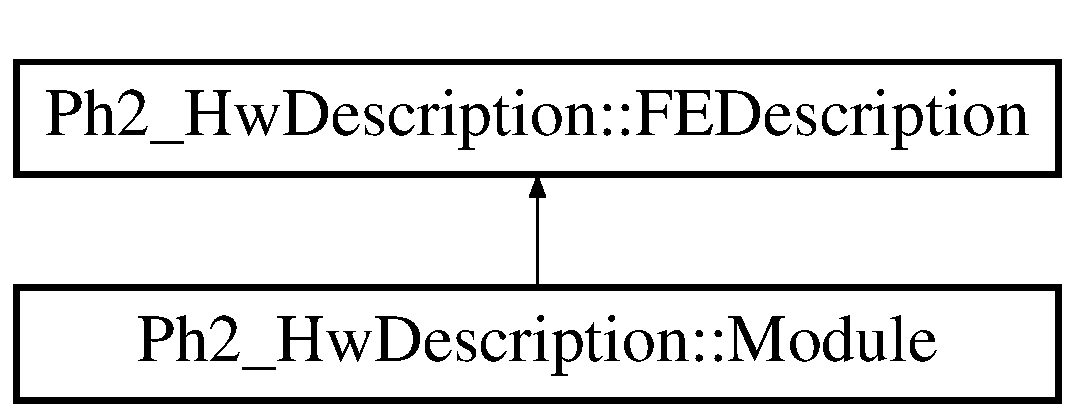
\includegraphics[height=2.000000cm]{class_ph2___hw_description_1_1_module}
\end{center}
\end{figure}
\subsection*{Public Member Functions}
\begin{DoxyCompactItemize}
\item 
\hyperlink{class_ph2___hw_description_1_1_module_adab1cde05b3a83e7199f5b55166074ed}{Module} (\hyperlink{class_ph2___hw_description_1_1_front_end_description}{Front\-End\-Description} \&p\-Fe\-Desc)
\item 
\hyperlink{class_ph2___hw_description_1_1_module_acb5e5f17c946438f985c209563060f26}{Module} (uint8\-\_\-t p\-Shelve\-Id, uint8\-\_\-t p\-Be\-Id, uint8\-\_\-t p\-F\-M\-C\-Id, uint8\-\_\-t p\-Fe\-Id, uint8\-\_\-t p\-Module\-Id)
\item 
\hyperlink{class_ph2___hw_description_1_1_module_aaec7dd439bdf7a1db3f2136569a00125}{Module} ()
\item 
\hyperlink{class_ph2___hw_description_1_1_module_a8142f34ea2308ed78e8d0dbb042bc5f3}{$\sim$\-Module} ()
\item 
uint8\-\_\-t \hyperlink{class_ph2___hw_description_1_1_module_a8703442b1055c0c38b4157fc155ac084}{get\-N\-Cbc} ()
\begin{DoxyCompactList}\small\item\em Get the number of \hyperlink{class_ph2___hw_description_1_1_cbc}{Cbc} connected to the \hyperlink{class_ph2___hw_description_1_1_module}{Module}. \end{DoxyCompactList}\item 
void \hyperlink{class_ph2___hw_description_1_1_module_ac2743d5056bc3053bf472e5fd94bbf14}{add\-Cbc} (\hyperlink{class_ph2___hw_description_1_1_cbc}{Cbc} \&p\-Cbc)
\begin{DoxyCompactList}\small\item\em Adding a \hyperlink{class_ph2___hw_description_1_1_cbc}{Cbc} to the vector. \end{DoxyCompactList}\item 
bool \hyperlink{class_ph2___hw_description_1_1_module_a0aa7c940311bd13a32fd4e0f251c2d27}{remove\-Cbc} (uint8\-\_\-t p\-Cbc\-Id)
\begin{DoxyCompactList}\small\item\em Remove a \hyperlink{class_ph2___hw_description_1_1_cbc}{Cbc} from the vector. \end{DoxyCompactList}\item 
\hyperlink{class_ph2___hw_description_1_1_cbc}{Cbc} $\ast$ \hyperlink{class_ph2___hw_description_1_1_module_a05ccbee9ca3eb8022e359b5e9dabe783}{get\-Cbc} (uint8\-\_\-t p\-Cbc\-Id)
\begin{DoxyCompactList}\small\item\em Get a \hyperlink{class_ph2___hw_description_1_1_cbc}{Cbc} from the vector. \end{DoxyCompactList}\end{DoxyCompactItemize}
\subsection*{Data Fields}
\begin{DoxyCompactItemize}
\item 
uint8\-\_\-t \hyperlink{class_ph2___hw_description_1_1_module_a8bf42ae708d304acbc5509edf7f7cee0}{f\-Module\-Id}
\end{DoxyCompactItemize}
\subsection*{Protected Attributes}
\begin{DoxyCompactItemize}
\item 
std\-::vector$<$ \hyperlink{class_ph2___hw_description_1_1_cbc}{Cbc} $>$ \hyperlink{class_ph2___hw_description_1_1_module_ab5cfd93bf927592f609d31f66cd4161b}{f\-Cbc\-Vector}
\end{DoxyCompactItemize}


\subsection{Detailed Description}
contains a vector of \hyperlink{class_ph2___hw_description_1_1_cbc}{Cbc} which are connected to the \hyperlink{class_ph2___hw_description_1_1_module}{Module} 

\subsection{Constructor \& Destructor Documentation}
\hypertarget{class_ph2___hw_description_1_1_module_adab1cde05b3a83e7199f5b55166074ed}{\index{Ph2\-\_\-\-Hw\-Description\-::\-Module@{Ph2\-\_\-\-Hw\-Description\-::\-Module}!Module@{Module}}
\index{Module@{Module}!Ph2_HwDescription::Module@{Ph2\-\_\-\-Hw\-Description\-::\-Module}}
\subsubsection[{Module}]{\setlength{\rightskip}{0pt plus 5cm}Ph2\-\_\-\-Hw\-Description\-::\-Module\-::\-Module (
\begin{DoxyParamCaption}
\item[{{\bf Front\-End\-Description} \&}]{p\-Fe\-Desc}
\end{DoxyParamCaption}
)}}\label{class_ph2___hw_description_1_1_module_adab1cde05b3a83e7199f5b55166074ed}
\hypertarget{class_ph2___hw_description_1_1_module_acb5e5f17c946438f985c209563060f26}{\index{Ph2\-\_\-\-Hw\-Description\-::\-Module@{Ph2\-\_\-\-Hw\-Description\-::\-Module}!Module@{Module}}
\index{Module@{Module}!Ph2_HwDescription::Module@{Ph2\-\_\-\-Hw\-Description\-::\-Module}}
\subsubsection[{Module}]{\setlength{\rightskip}{0pt plus 5cm}Ph2\-\_\-\-Hw\-Description\-::\-Module\-::\-Module (
\begin{DoxyParamCaption}
\item[{uint8\-\_\-t}]{p\-Shelve\-Id, }
\item[{uint8\-\_\-t}]{p\-Be\-Id, }
\item[{uint8\-\_\-t}]{p\-F\-M\-C\-Id, }
\item[{uint8\-\_\-t}]{p\-Fe\-Id, }
\item[{uint8\-\_\-t}]{p\-Module\-Id}
\end{DoxyParamCaption}
)}}\label{class_ph2___hw_description_1_1_module_acb5e5f17c946438f985c209563060f26}
\hypertarget{class_ph2___hw_description_1_1_module_aaec7dd439bdf7a1db3f2136569a00125}{\index{Ph2\-\_\-\-Hw\-Description\-::\-Module@{Ph2\-\_\-\-Hw\-Description\-::\-Module}!Module@{Module}}
\index{Module@{Module}!Ph2_HwDescription::Module@{Ph2\-\_\-\-Hw\-Description\-::\-Module}}
\subsubsection[{Module}]{\setlength{\rightskip}{0pt plus 5cm}Ph2\-\_\-\-Hw\-Description\-::\-Module\-::\-Module (
\begin{DoxyParamCaption}
{}
\end{DoxyParamCaption}
)}}\label{class_ph2___hw_description_1_1_module_aaec7dd439bdf7a1db3f2136569a00125}
\hypertarget{class_ph2___hw_description_1_1_module_a8142f34ea2308ed78e8d0dbb042bc5f3}{\index{Ph2\-\_\-\-Hw\-Description\-::\-Module@{Ph2\-\_\-\-Hw\-Description\-::\-Module}!$\sim$\-Module@{$\sim$\-Module}}
\index{$\sim$\-Module@{$\sim$\-Module}!Ph2_HwDescription::Module@{Ph2\-\_\-\-Hw\-Description\-::\-Module}}
\subsubsection[{$\sim$\-Module}]{\setlength{\rightskip}{0pt plus 5cm}Ph2\-\_\-\-Hw\-Description\-::\-Module\-::$\sim$\-Module (
\begin{DoxyParamCaption}
{}
\end{DoxyParamCaption}
)\hspace{0.3cm}{\ttfamily [inline]}}}\label{class_ph2___hw_description_1_1_module_a8142f34ea2308ed78e8d0dbb042bc5f3}


\subsection{Member Function Documentation}
\hypertarget{class_ph2___hw_description_1_1_module_ac2743d5056bc3053bf472e5fd94bbf14}{\index{Ph2\-\_\-\-Hw\-Description\-::\-Module@{Ph2\-\_\-\-Hw\-Description\-::\-Module}!add\-Cbc@{add\-Cbc}}
\index{add\-Cbc@{add\-Cbc}!Ph2_HwDescription::Module@{Ph2\-\_\-\-Hw\-Description\-::\-Module}}
\subsubsection[{add\-Cbc}]{\setlength{\rightskip}{0pt plus 5cm}void Ph2\-\_\-\-Hw\-Description\-::\-Module\-::add\-Cbc (
\begin{DoxyParamCaption}
\item[{{\bf Cbc} \&}]{p\-Cbc}
\end{DoxyParamCaption}
)}}\label{class_ph2___hw_description_1_1_module_ac2743d5056bc3053bf472e5fd94bbf14}


Adding a \hyperlink{class_ph2___hw_description_1_1_cbc}{Cbc} to the vector. 


\begin{DoxyParams}{Parameters}
{\em p\-Cbc} & \\
\hline
\end{DoxyParams}
\hypertarget{class_ph2___hw_description_1_1_module_a05ccbee9ca3eb8022e359b5e9dabe783}{\index{Ph2\-\_\-\-Hw\-Description\-::\-Module@{Ph2\-\_\-\-Hw\-Description\-::\-Module}!get\-Cbc@{get\-Cbc}}
\index{get\-Cbc@{get\-Cbc}!Ph2_HwDescription::Module@{Ph2\-\_\-\-Hw\-Description\-::\-Module}}
\subsubsection[{get\-Cbc}]{\setlength{\rightskip}{0pt plus 5cm}{\bf Cbc} $\ast$ Ph2\-\_\-\-Hw\-Description\-::\-Module\-::get\-Cbc (
\begin{DoxyParamCaption}
\item[{uint8\-\_\-t}]{p\-Cbc\-Id}
\end{DoxyParamCaption}
)}}\label{class_ph2___hw_description_1_1_module_a05ccbee9ca3eb8022e359b5e9dabe783}


Get a \hyperlink{class_ph2___hw_description_1_1_cbc}{Cbc} from the vector. 


\begin{DoxyParams}{Parameters}
{\em p\-Cbc\-Id} & \\
\hline
\end{DoxyParams}
\begin{DoxyReturn}{Returns}
a pointer of \hyperlink{class_ph2___hw_description_1_1_cbc}{Cbc}, so we can manipulate directly the \hyperlink{class_ph2___hw_description_1_1_cbc}{Cbc} contained in the vector 
\end{DoxyReturn}
\hypertarget{class_ph2___hw_description_1_1_module_a8703442b1055c0c38b4157fc155ac084}{\index{Ph2\-\_\-\-Hw\-Description\-::\-Module@{Ph2\-\_\-\-Hw\-Description\-::\-Module}!get\-N\-Cbc@{get\-N\-Cbc}}
\index{get\-N\-Cbc@{get\-N\-Cbc}!Ph2_HwDescription::Module@{Ph2\-\_\-\-Hw\-Description\-::\-Module}}
\subsubsection[{get\-N\-Cbc}]{\setlength{\rightskip}{0pt plus 5cm}uint8\-\_\-t Ph2\-\_\-\-Hw\-Description\-::\-Module\-::get\-N\-Cbc (
\begin{DoxyParamCaption}
{}
\end{DoxyParamCaption}
)\hspace{0.3cm}{\ttfamily [inline]}}}\label{class_ph2___hw_description_1_1_module_a8703442b1055c0c38b4157fc155ac084}


Get the number of \hyperlink{class_ph2___hw_description_1_1_cbc}{Cbc} connected to the \hyperlink{class_ph2___hw_description_1_1_module}{Module}. 

\begin{DoxyReturn}{Returns}
The size of the vector 
\end{DoxyReturn}
\hypertarget{class_ph2___hw_description_1_1_module_a0aa7c940311bd13a32fd4e0f251c2d27}{\index{Ph2\-\_\-\-Hw\-Description\-::\-Module@{Ph2\-\_\-\-Hw\-Description\-::\-Module}!remove\-Cbc@{remove\-Cbc}}
\index{remove\-Cbc@{remove\-Cbc}!Ph2_HwDescription::Module@{Ph2\-\_\-\-Hw\-Description\-::\-Module}}
\subsubsection[{remove\-Cbc}]{\setlength{\rightskip}{0pt plus 5cm}bool Ph2\-\_\-\-Hw\-Description\-::\-Module\-::remove\-Cbc (
\begin{DoxyParamCaption}
\item[{uint8\-\_\-t}]{p\-Cbc\-Id}
\end{DoxyParamCaption}
)}}\label{class_ph2___hw_description_1_1_module_a0aa7c940311bd13a32fd4e0f251c2d27}


Remove a \hyperlink{class_ph2___hw_description_1_1_cbc}{Cbc} from the vector. 


\begin{DoxyParams}{Parameters}
{\em p\-Cbc\-Id} & \\
\hline
\end{DoxyParams}
\begin{DoxyReturn}{Returns}
a bool which indicate if the removing was successful 
\end{DoxyReturn}


\subsection{Field Documentation}
\hypertarget{class_ph2___hw_description_1_1_module_ab5cfd93bf927592f609d31f66cd4161b}{\index{Ph2\-\_\-\-Hw\-Description\-::\-Module@{Ph2\-\_\-\-Hw\-Description\-::\-Module}!f\-Cbc\-Vector@{f\-Cbc\-Vector}}
\index{f\-Cbc\-Vector@{f\-Cbc\-Vector}!Ph2_HwDescription::Module@{Ph2\-\_\-\-Hw\-Description\-::\-Module}}
\subsubsection[{f\-Cbc\-Vector}]{\setlength{\rightskip}{0pt plus 5cm}std\-::vector$<$ {\bf Cbc} $>$ Ph2\-\_\-\-Hw\-Description\-::\-Module\-::f\-Cbc\-Vector\hspace{0.3cm}{\ttfamily [protected]}}}\label{class_ph2___hw_description_1_1_module_ab5cfd93bf927592f609d31f66cd4161b}
\hypertarget{class_ph2___hw_description_1_1_module_a8bf42ae708d304acbc5509edf7f7cee0}{\index{Ph2\-\_\-\-Hw\-Description\-::\-Module@{Ph2\-\_\-\-Hw\-Description\-::\-Module}!f\-Module\-Id@{f\-Module\-Id}}
\index{f\-Module\-Id@{f\-Module\-Id}!Ph2_HwDescription::Module@{Ph2\-\_\-\-Hw\-Description\-::\-Module}}
\subsubsection[{f\-Module\-Id}]{\setlength{\rightskip}{0pt plus 5cm}uint8\-\_\-t Ph2\-\_\-\-Hw\-Description\-::\-Module\-::f\-Module\-Id}}\label{class_ph2___hw_description_1_1_module_a8bf42ae708d304acbc5509edf7f7cee0}


The documentation for this class was generated from the following files\-:\begin{DoxyCompactItemize}
\item 
H\-W\-Description/\hyperlink{_module_8h}{Module.\-h}\item 
H\-W\-Description/\hyperlink{_module_8cc}{Module.\-cc}\end{DoxyCompactItemize}

\hypertarget{class_ph2___hw_interface_1_1_reg_manager}{\section{Ph2\-\_\-\-Hw\-Interface\-:\-:Reg\-Manager Class Reference}
\label{class_ph2___hw_interface_1_1_reg_manager}\index{Ph2\-\_\-\-Hw\-Interface\-::\-Reg\-Manager@{Ph2\-\_\-\-Hw\-Interface\-::\-Reg\-Manager}}
}


Permit connection to given boards and r/w given registers.  




{\ttfamily \#include $<$Reg\-Manager.\-h$>$}

Inheritance diagram for Ph2\-\_\-\-Hw\-Interface\-:\-:Reg\-Manager\-:\begin{figure}[H]
\begin{center}
\leavevmode
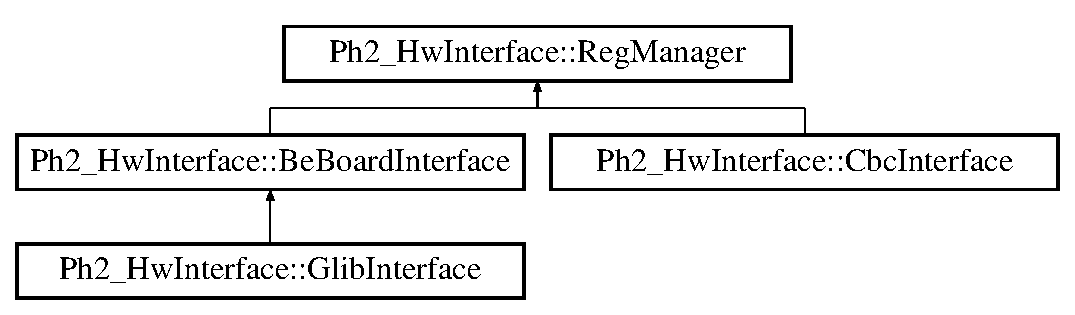
\includegraphics[height=2.000000cm]{class_ph2___hw_interface_1_1_reg_manager}
\end{center}
\end{figure}
\subsection*{Public Member Functions}
\begin{DoxyCompactItemize}
\item 
\hyperlink{class_ph2___hw_interface_1_1_reg_manager_a938f6b582b1fffcb478f35fd9d81954f}{Reg\-Manager} (const char $\ast$pu\-Hal\-Config\-File\-Name)
\begin{DoxyCompactList}\small\item\em Constructor of the \hyperlink{class_ph2___hw_interface_1_1_reg_manager}{Reg\-Manager} class. \end{DoxyCompactList}\item 
virtual \hyperlink{class_ph2___hw_interface_1_1_reg_manager_a5d650c4e6467153f98f999abbbfc354c}{$\sim$\-Reg\-Manager} ()
\begin{DoxyCompactList}\small\item\em Destructor of the \hyperlink{class_ph2___hw_interface_1_1_reg_manager}{Reg\-Manager} class. \end{DoxyCompactList}\end{DoxyCompactItemize}
\subsection*{Protected Member Functions}
\begin{DoxyCompactItemize}
\item 
virtual bool \hyperlink{class_ph2___hw_interface_1_1_reg_manager_a31174516fef6706c88c3f59dd93e4fdf}{Write\-Reg} (const std\-::string \&p\-Reg\-Node, const uint32\-\_\-t \&p\-Val)
\begin{DoxyCompactList}\small\item\em Write a register. \end{DoxyCompactList}\item 
virtual bool \hyperlink{class_ph2___hw_interface_1_1_reg_manager_a888f5cccb05daa28896cf622abfdcbd6}{Write\-Block\-Reg} (const std\-::string \&p\-Reg\-Node, const std\-::vector$<$ uint32\-\_\-t $>$ \&p\-Values)
\begin{DoxyCompactList}\small\item\em Write a block of values in a register. \end{DoxyCompactList}\item 
virtual uhal\-::\-Val\-Word$<$ uint32\-\_\-t $>$ \hyperlink{class_ph2___hw_interface_1_1_reg_manager_a077e0a18592206365150680213345112}{Read\-Reg} (const std\-::string \&p\-Reg\-Node)
\begin{DoxyCompactList}\small\item\em Read a value in a register. \end{DoxyCompactList}\item 
virtual uhal\-::\-Val\-Vector$<$ uint32\-\_\-t $>$ \hyperlink{class_ph2___hw_interface_1_1_reg_manager_a6481c211d27badc409ff0e7af20575e4}{Read\-Block\-Reg} (const std\-::string \&p\-Reg\-Node, const uint32\-\_\-t \&p\-Blocksize)
\begin{DoxyCompactList}\small\item\em Read a block of values in a register. \end{DoxyCompactList}\item 
virtual void \hyperlink{class_ph2___hw_interface_1_1_reg_manager_a20c502bcad5115c6ae16d4d356b72f0c}{Choose\-Board} (uint8\-\_\-t p\-Board\-Id)
\begin{DoxyCompactList}\small\item\em Choose the board we want to talk with. \end{DoxyCompactList}\end{DoxyCompactItemize}
\subsection*{Protected Attributes}
\begin{DoxyCompactItemize}
\item 
uhal\-::\-Hw\-Interface $\ast$ \hyperlink{class_ph2___hw_interface_1_1_reg_manager_a0d4908ec834a3a0b7d8139872fd0a4a0}{f\-Board}
\item 
const char $\ast$ \hyperlink{class_ph2___hw_interface_1_1_reg_manager_aaaa29ca65c283acc645132c7bef0f24f}{f\-U\-Hal\-Config\-File\-Name}
\item 
std\-::map$<$ uint8\-\_\-t, \\*
uhal\-::\-Hw\-Interface $\ast$ $>$ \hyperlink{class_ph2___hw_interface_1_1_reg_manager_a9c34ffe467a572796c05036533bb6d39}{f\-Board\-Map}
\end{DoxyCompactItemize}


\subsection{Detailed Description}
Permit connection to given boards and r/w given registers. 

\subsection{Constructor \& Destructor Documentation}
\hypertarget{class_ph2___hw_interface_1_1_reg_manager_a938f6b582b1fffcb478f35fd9d81954f}{\index{Ph2\-\_\-\-Hw\-Interface\-::\-Reg\-Manager@{Ph2\-\_\-\-Hw\-Interface\-::\-Reg\-Manager}!Reg\-Manager@{Reg\-Manager}}
\index{Reg\-Manager@{Reg\-Manager}!Ph2_HwInterface::RegManager@{Ph2\-\_\-\-Hw\-Interface\-::\-Reg\-Manager}}
\subsubsection[{Reg\-Manager}]{\setlength{\rightskip}{0pt plus 5cm}Ph2\-\_\-\-Hw\-Interface\-::\-Reg\-Manager\-::\-Reg\-Manager (
\begin{DoxyParamCaption}
\item[{const char $\ast$}]{pu\-Hal\-Config\-File\-Name}
\end{DoxyParamCaption}
)}}\label{class_ph2___hw_interface_1_1_reg_manager_a938f6b582b1fffcb478f35fd9d81954f}


Constructor of the \hyperlink{class_ph2___hw_interface_1_1_reg_manager}{Reg\-Manager} class. 


\begin{DoxyParams}{Parameters}
{\em pu\-Hal\-Config\-File\-Name} & \-: path of the u\-Hal Config File \\
\hline
\end{DoxyParams}
\hypertarget{class_ph2___hw_interface_1_1_reg_manager_a5d650c4e6467153f98f999abbbfc354c}{\index{Ph2\-\_\-\-Hw\-Interface\-::\-Reg\-Manager@{Ph2\-\_\-\-Hw\-Interface\-::\-Reg\-Manager}!$\sim$\-Reg\-Manager@{$\sim$\-Reg\-Manager}}
\index{$\sim$\-Reg\-Manager@{$\sim$\-Reg\-Manager}!Ph2_HwInterface::RegManager@{Ph2\-\_\-\-Hw\-Interface\-::\-Reg\-Manager}}
\subsubsection[{$\sim$\-Reg\-Manager}]{\setlength{\rightskip}{0pt plus 5cm}Ph2\-\_\-\-Hw\-Interface\-::\-Reg\-Manager\-::$\sim$\-Reg\-Manager (
\begin{DoxyParamCaption}
{}
\end{DoxyParamCaption}
)\hspace{0.3cm}{\ttfamily [virtual]}}}\label{class_ph2___hw_interface_1_1_reg_manager_a5d650c4e6467153f98f999abbbfc354c}


Destructor of the \hyperlink{class_ph2___hw_interface_1_1_reg_manager}{Reg\-Manager} class. 



\subsection{Member Function Documentation}
\hypertarget{class_ph2___hw_interface_1_1_reg_manager_a20c502bcad5115c6ae16d4d356b72f0c}{\index{Ph2\-\_\-\-Hw\-Interface\-::\-Reg\-Manager@{Ph2\-\_\-\-Hw\-Interface\-::\-Reg\-Manager}!Choose\-Board@{Choose\-Board}}
\index{Choose\-Board@{Choose\-Board}!Ph2_HwInterface::RegManager@{Ph2\-\_\-\-Hw\-Interface\-::\-Reg\-Manager}}
\subsubsection[{Choose\-Board}]{\setlength{\rightskip}{0pt plus 5cm}void Ph2\-\_\-\-Hw\-Interface\-::\-Reg\-Manager\-::\-Choose\-Board (
\begin{DoxyParamCaption}
\item[{uint8\-\_\-t}]{p\-Board\-Id}
\end{DoxyParamCaption}
)\hspace{0.3cm}{\ttfamily [protected]}, {\ttfamily [virtual]}}}\label{class_ph2___hw_interface_1_1_reg_manager_a20c502bcad5115c6ae16d4d356b72f0c}


Choose the board we want to talk with. 


\begin{DoxyParams}{Parameters}
{\em p\-Board\-Id} & \-: Id of the Board to connect to \\
\hline
\end{DoxyParams}
\hypertarget{class_ph2___hw_interface_1_1_reg_manager_a6481c211d27badc409ff0e7af20575e4}{\index{Ph2\-\_\-\-Hw\-Interface\-::\-Reg\-Manager@{Ph2\-\_\-\-Hw\-Interface\-::\-Reg\-Manager}!Read\-Block\-Reg@{Read\-Block\-Reg}}
\index{Read\-Block\-Reg@{Read\-Block\-Reg}!Ph2_HwInterface::RegManager@{Ph2\-\_\-\-Hw\-Interface\-::\-Reg\-Manager}}
\subsubsection[{Read\-Block\-Reg}]{\setlength{\rightskip}{0pt plus 5cm}uhal\-::\-Val\-Vector$<$ uint32\-\_\-t $>$ Ph2\-\_\-\-Hw\-Interface\-::\-Reg\-Manager\-::\-Read\-Block\-Reg (
\begin{DoxyParamCaption}
\item[{const std\-::string \&}]{p\-Reg\-Node, }
\item[{const uint32\-\_\-t \&}]{p\-Blocksize}
\end{DoxyParamCaption}
)\hspace{0.3cm}{\ttfamily [protected]}, {\ttfamily [virtual]}}}\label{class_ph2___hw_interface_1_1_reg_manager_a6481c211d27badc409ff0e7af20575e4}


Read a block of values in a register. 


\begin{DoxyParams}{Parameters}
{\em p\-Reg\-Node} & \-: Node of the register to read \\
\hline
{\em p\-Blocksize} & \-: Size of the block to read \\
\hline
\end{DoxyParams}
\begin{DoxyReturn}{Returns}
Val\-Vector block values of the register 
\end{DoxyReturn}
\hypertarget{class_ph2___hw_interface_1_1_reg_manager_a077e0a18592206365150680213345112}{\index{Ph2\-\_\-\-Hw\-Interface\-::\-Reg\-Manager@{Ph2\-\_\-\-Hw\-Interface\-::\-Reg\-Manager}!Read\-Reg@{Read\-Reg}}
\index{Read\-Reg@{Read\-Reg}!Ph2_HwInterface::RegManager@{Ph2\-\_\-\-Hw\-Interface\-::\-Reg\-Manager}}
\subsubsection[{Read\-Reg}]{\setlength{\rightskip}{0pt plus 5cm}uhal\-::\-Val\-Word$<$ uint32\-\_\-t $>$ Ph2\-\_\-\-Hw\-Interface\-::\-Reg\-Manager\-::\-Read\-Reg (
\begin{DoxyParamCaption}
\item[{const std\-::string \&}]{p\-Reg\-Node}
\end{DoxyParamCaption}
)\hspace{0.3cm}{\ttfamily [protected]}, {\ttfamily [virtual]}}}\label{class_ph2___hw_interface_1_1_reg_manager_a077e0a18592206365150680213345112}


Read a value in a register. 


\begin{DoxyParams}{Parameters}
{\em p\-Reg\-Node} & \-: Node of the register to read \\
\hline
\end{DoxyParams}
\begin{DoxyReturn}{Returns}
Val\-Word value of the register 
\end{DoxyReturn}
\hypertarget{class_ph2___hw_interface_1_1_reg_manager_a888f5cccb05daa28896cf622abfdcbd6}{\index{Ph2\-\_\-\-Hw\-Interface\-::\-Reg\-Manager@{Ph2\-\_\-\-Hw\-Interface\-::\-Reg\-Manager}!Write\-Block\-Reg@{Write\-Block\-Reg}}
\index{Write\-Block\-Reg@{Write\-Block\-Reg}!Ph2_HwInterface::RegManager@{Ph2\-\_\-\-Hw\-Interface\-::\-Reg\-Manager}}
\subsubsection[{Write\-Block\-Reg}]{\setlength{\rightskip}{0pt plus 5cm}bool Ph2\-\_\-\-Hw\-Interface\-::\-Reg\-Manager\-::\-Write\-Block\-Reg (
\begin{DoxyParamCaption}
\item[{const std\-::string \&}]{p\-Reg\-Node, }
\item[{const std\-::vector$<$ uint32\-\_\-t $>$ \&}]{p\-Values}
\end{DoxyParamCaption}
)\hspace{0.3cm}{\ttfamily [protected]}, {\ttfamily [virtual]}}}\label{class_ph2___hw_interface_1_1_reg_manager_a888f5cccb05daa28896cf622abfdcbd6}


Write a block of values in a register. 


\begin{DoxyParams}{Parameters}
{\em p\-Reg\-Node} & \-: Node of the register to write \\
\hline
{\em p\-Values} & \-: Block of values to write \\
\hline
\end{DoxyParams}
\begin{DoxyReturn}{Returns}
boolean confirming the writing 
\end{DoxyReturn}
\hypertarget{class_ph2___hw_interface_1_1_reg_manager_a31174516fef6706c88c3f59dd93e4fdf}{\index{Ph2\-\_\-\-Hw\-Interface\-::\-Reg\-Manager@{Ph2\-\_\-\-Hw\-Interface\-::\-Reg\-Manager}!Write\-Reg@{Write\-Reg}}
\index{Write\-Reg@{Write\-Reg}!Ph2_HwInterface::RegManager@{Ph2\-\_\-\-Hw\-Interface\-::\-Reg\-Manager}}
\subsubsection[{Write\-Reg}]{\setlength{\rightskip}{0pt plus 5cm}bool Ph2\-\_\-\-Hw\-Interface\-::\-Reg\-Manager\-::\-Write\-Reg (
\begin{DoxyParamCaption}
\item[{const std\-::string \&}]{p\-Reg\-Node, }
\item[{const uint32\-\_\-t \&}]{p\-Val}
\end{DoxyParamCaption}
)\hspace{0.3cm}{\ttfamily [protected]}, {\ttfamily [virtual]}}}\label{class_ph2___hw_interface_1_1_reg_manager_a31174516fef6706c88c3f59dd93e4fdf}


Write a register. 


\begin{DoxyParams}{Parameters}
{\em p\-Reg\-Node} & \-: Node of the register to write \\
\hline
{\em p\-Val} & \-: Value to write \\
\hline
\end{DoxyParams}
\begin{DoxyReturn}{Returns}
boolean confirming the writing 
\end{DoxyReturn}


\subsection{Field Documentation}
\hypertarget{class_ph2___hw_interface_1_1_reg_manager_a0d4908ec834a3a0b7d8139872fd0a4a0}{\index{Ph2\-\_\-\-Hw\-Interface\-::\-Reg\-Manager@{Ph2\-\_\-\-Hw\-Interface\-::\-Reg\-Manager}!f\-Board@{f\-Board}}
\index{f\-Board@{f\-Board}!Ph2_HwInterface::RegManager@{Ph2\-\_\-\-Hw\-Interface\-::\-Reg\-Manager}}
\subsubsection[{f\-Board}]{\setlength{\rightskip}{0pt plus 5cm}uhal\-::\-Hw\-Interface$\ast$ Ph2\-\_\-\-Hw\-Interface\-::\-Reg\-Manager\-::f\-Board\hspace{0.3cm}{\ttfamily [protected]}}}\label{class_ph2___hw_interface_1_1_reg_manager_a0d4908ec834a3a0b7d8139872fd0a4a0}
Board in use \hypertarget{class_ph2___hw_interface_1_1_reg_manager_a9c34ffe467a572796c05036533bb6d39}{\index{Ph2\-\_\-\-Hw\-Interface\-::\-Reg\-Manager@{Ph2\-\_\-\-Hw\-Interface\-::\-Reg\-Manager}!f\-Board\-Map@{f\-Board\-Map}}
\index{f\-Board\-Map@{f\-Board\-Map}!Ph2_HwInterface::RegManager@{Ph2\-\_\-\-Hw\-Interface\-::\-Reg\-Manager}}
\subsubsection[{f\-Board\-Map}]{\setlength{\rightskip}{0pt plus 5cm}std\-::map$<$uint8\-\_\-t,uhal\-::\-Hw\-Interface$\ast$$>$ Ph2\-\_\-\-Hw\-Interface\-::\-Reg\-Manager\-::f\-Board\-Map\hspace{0.3cm}{\ttfamily [protected]}}}\label{class_ph2___hw_interface_1_1_reg_manager_a9c34ffe467a572796c05036533bb6d39}
Board Map with all known boards \hypertarget{class_ph2___hw_interface_1_1_reg_manager_aaaa29ca65c283acc645132c7bef0f24f}{\index{Ph2\-\_\-\-Hw\-Interface\-::\-Reg\-Manager@{Ph2\-\_\-\-Hw\-Interface\-::\-Reg\-Manager}!f\-U\-Hal\-Config\-File\-Name@{f\-U\-Hal\-Config\-File\-Name}}
\index{f\-U\-Hal\-Config\-File\-Name@{f\-U\-Hal\-Config\-File\-Name}!Ph2_HwInterface::RegManager@{Ph2\-\_\-\-Hw\-Interface\-::\-Reg\-Manager}}
\subsubsection[{f\-U\-Hal\-Config\-File\-Name}]{\setlength{\rightskip}{0pt plus 5cm}const char$\ast$ Ph2\-\_\-\-Hw\-Interface\-::\-Reg\-Manager\-::f\-U\-Hal\-Config\-File\-Name\hspace{0.3cm}{\ttfamily [protected]}}}\label{class_ph2___hw_interface_1_1_reg_manager_aaaa29ca65c283acc645132c7bef0f24f}
path of the u\-Hal Config File 

The documentation for this class was generated from the following files\-:\begin{DoxyCompactItemize}
\item 
H\-W\-Interface/\hyperlink{_reg_manager_8h}{Reg\-Manager.\-h}\item 
H\-W\-Interface/\hyperlink{_reg_manager_8cc}{Reg\-Manager.\-cc}\end{DoxyCompactItemize}

\chapter{File Documentation}
\hypertarget{_cbc_8cc}{
\section{HWDescription/Cbc.cc File Reference}
\label{_cbc_8cc}\index{HWDescription/Cbc.cc@{HWDescription/Cbc.cc}}
}
{\tt \#include \char`\"{}Cbc.h\char`\"{}}\par
{\tt \#include $<$fstream$>$}\par
{\tt \#include $<$cstdio$>$}\par
{\tt \#include $<$sstream$>$}\par
{\tt \#include $<$iostream$>$}\par
{\tt \#include $<$string.h$>$}\par
{\tt \#include $<$iomanip$>$}\par
{\tt \#include \char`\"{}Definition.h\char`\"{}}\par
\subsection*{Namespaces}
\begin{CompactItemize}
\item 
namespace \hyperlink{namespace_ph2___hw_description}{Ph2\_\-Hw\-Description}
\end{CompactItemize}

\hypertarget{_cbc_8h}{\section{H\-W\-Description/\-Cbc.h File Reference}
\label{_cbc_8h}\index{H\-W\-Description/\-Cbc.\-h@{H\-W\-Description/\-Cbc.\-h}}
}


Cbc Description class, config of the Cbcs.  


{\ttfamily \#include \char`\"{}Front\-End\-Description.\-h\char`\"{}}\\*
{\ttfamily \#include \char`\"{}Cbc\-Reg\-Item.\-h\char`\"{}}\\*
{\ttfamily \#include $<$iostream$>$}\\*
{\ttfamily \#include $<$map$>$}\\*
{\ttfamily \#include $<$string$>$}\\*
{\ttfamily \#include $<$boost/cstdint.\-hpp$>$}\\*
\subsection*{Data Structures}
\begin{DoxyCompactItemize}
\item 
class \hyperlink{class_ph2___hw_description_1_1_cbc}{Ph2\-\_\-\-Hw\-Description\-::\-Cbc}
\begin{DoxyCompactList}\small\item\em Read/\-Write \hyperlink{class_ph2___hw_description_1_1_cbc}{Cbc}'s registers on a file. \end{DoxyCompactList}\item 
struct \hyperlink{struct_ph2___hw_description_1_1_cbc_comparer}{Ph2\-\_\-\-Hw\-Description\-::\-Cbc\-Comparer}
\begin{DoxyCompactList}\small\item\em Compare two \hyperlink{class_ph2___hw_description_1_1_cbc}{Cbc} by their I\-D. \end{DoxyCompactList}\end{DoxyCompactItemize}
\subsection*{Namespaces}
\begin{DoxyCompactItemize}
\item 
\hyperlink{namespace_ph2___hw_description}{Ph2\-\_\-\-Hw\-Description}
\begin{DoxyCompactList}\small\item\em Namespace regrouping all the hardware description. \end{DoxyCompactList}\end{DoxyCompactItemize}
\subsection*{Macros}
\begin{DoxyCompactItemize}
\item 
\#define \hyperlink{_cbc_8h_ad406c895476128d696804038e617141b}{default\-\_\-file}~\char`\"{}default\-\_\-file.\-txt\char`\"{}
\end{DoxyCompactItemize}
\subsection*{Typedefs}
\begin{DoxyCompactItemize}
\item 
typedef std\-::map$<$ std\-::string, \\*
Cbc\-Reg\-Item $>$ \hyperlink{namespace_ph2___hw_description_a9a23b373068f169aa67ca1d22c9a6001}{Ph2\-\_\-\-Hw\-Description\-::\-Cbc\-Reg\-Map}
\end{DoxyCompactItemize}


\subsection{Detailed Description}
Cbc Description class, config of the Cbcs. \begin{DoxyAuthor}{Author}
Lorenzo B\-I\-D\-E\-G\-A\-I\-N 
\end{DoxyAuthor}
\begin{DoxyDate}{Date}
25/06/14
\end{DoxyDate}
Support \-: mail to \-: \href{mailto:lorenzo.bidegain@cern.ch}{\tt lorenzo.\-bidegain@cern.\-ch} 

\subsection{Macro Definition Documentation}
\hypertarget{_cbc_8h_ad406c895476128d696804038e617141b}{\index{Cbc.\-h@{Cbc.\-h}!default\-\_\-file@{default\-\_\-file}}
\index{default\-\_\-file@{default\-\_\-file}!Cbc.h@{Cbc.\-h}}
\subsubsection[{default\-\_\-file}]{\setlength{\rightskip}{0pt plus 5cm}\#define default\-\_\-file~\char`\"{}default\-\_\-file.\-txt\char`\"{}}}\label{_cbc_8h_ad406c895476128d696804038e617141b}

\hypertarget{_cbc_reg_item_8h}{\section{H\-W\-Description/\-Cbc\-Reg\-Item.h File Reference}
\label{_cbc_reg_item_8h}\index{H\-W\-Description/\-Cbc\-Reg\-Item.\-h@{H\-W\-Description/\-Cbc\-Reg\-Item.\-h}}
}
\subsection*{Data Structures}
\begin{DoxyCompactItemize}
\item 
struct \hyperlink{struct_ph2___hw_description_1_1_cbc_reg_item}{Ph2\-\_\-\-Hw\-Description\-::\-Cbc\-Reg\-Item}
\item 
struct \hyperlink{struct_ph2___hw_description_1_1_reg_item_comparer}{Ph2\-\_\-\-Hw\-Description\-::\-Reg\-Item\-Comparer}
\end{DoxyCompactItemize}
\subsection*{Namespaces}
\begin{DoxyCompactItemize}
\item 
\hyperlink{namespace_ph2___hw_description}{Ph2\-\_\-\-Hw\-Description}
\end{DoxyCompactItemize}

\hypertarget{_definition_8h}{
\section{HWDescription/Definition.h File Reference}
\label{_definition_8h}\index{HWDescription/Definition.h@{HWDescription/Definition.h}}
}
\subsection*{Defines}
\begin{CompactItemize}
\item 
\#define \hyperlink{_definition_8h_522d1a46e55b54c8ff9ec3275c60d73a}{XML\_\-DESCRIPTION\_\-FILE\_\-2CBC}~\char`\"{}settings/HWDescription\_\-2CBC.xml\char`\"{}
\item 
\#define \hyperlink{_definition_8h_26d84c24d1a2341a0fa6d42a89921628}{XML\_\-DESCRIPTION\_\-FILE\_\-8CBC}~\char`\"{}settings/HWDescription\_\-8CBC.xml\char`\"{}
\item 
\#define \hyperlink{_definition_8h_7538d40fca6562ecc1768f6d07cef2fa}{I2C\_\-CTRL\_\-ENABLE}~0x000009F4
\item 
\#define \hyperlink{_definition_8h_b1dd2d69bec1712857cc2a103c85c26d}{I2C\_\-CTRL\_\-DISABLE}~0
\item 
\#define \hyperlink{_definition_8h_8d3f448d28b023f560e3df976bb3ff9c}{I2C\_\-STROBE}~1
\item 
\#define \hyperlink{_definition_8h_ae239b4919cbd8d8dced934150986de3}{I2C\_\-M16B}~0
\item 
\#define \hyperlink{_definition_8h_c030aa7b3fbd8b2432a9c66fc49fc4ae}{I2C\_\-MEM}~1
\item 
\#define \hyperlink{_definition_8h_7978167075eb8954c1090fc7ce9647c6}{I2C\_\-WRITE\_\-ADDR}~0x09
\item 
\#define \hyperlink{_definition_8h_11a0148c64950f3315f38d957cd43d37}{I2C\_\-READ\_\-ADDR}~0x06
\item 
\#define \hyperlink{_definition_8h_b15137f7c592d05573de99f078516157}{I2C\_\-SLAVE}~0x5B
\item 
\#define \hyperlink{_definition_8h_e308275dafb538f2511ea285fea768d0}{I2C\_\-COMMAND}~\char`\"{}user\_\-wb\_\-ttc\_\-fmc\_\-regs.cbc\_\-reg\_\-i2c\_\-command\char`\"{}
\item 
\#define \hyperlink{_definition_8h_46aaa2293185dfc3cd655f65bea7f614}{I2C\_\-REPLY}~\char`\"{}user\_\-wb\_\-ttc\_\-fmc\_\-regs.cbc\_\-reg\_\-i2c\_\-reply\char`\"{}
\item 
\#define \hyperlink{_definition_8h_15db09e24617ea5c5843213672ac8a03}{I2C\_\-SETTINGS}~\char`\"{}user\_\-wb\_\-ttc\_\-fmc\_\-regs.cbc\_\-reg\_\-i2c\_\-settings\char`\"{}
\item 
\#define \hyperlink{_definition_8h_30957298974d3b5c605a9e6e3cf33ff9}{MAX\_\-NB\_\-LOOP}~50
\item 
\#define \hyperlink{_definition_8h_9b229c5fa667622ae84c26cbbfca2c4a}{BOARD\_\-TYPE}~\char`\"{}board\_\-id\char`\"{}
\item 
\#define \hyperlink{_definition_8h_5a209f781c62e738bb2f3868604fbe77}{FW\_\-VERSION\_\-MAJOR}~\char`\"{}firm\_\-id.firmware\_\-major\char`\"{}
\item 
\#define \hyperlink{_definition_8h_e224d2fae5df95eef5b8b1638b714731}{FW\_\-VERSION\_\-MINOR}~\char`\"{}firm\_\-id.firmware\_\-minor\char`\"{}
\item 
\#define \hyperlink{_definition_8h_46d23f1b70547c7ec03a7ede5a4a53c1}{FW\_\-VERSION\_\-BUILD}~\char`\"{}firm\_\-id.firmware\_\-build\char`\"{}
\item 
\#define \hyperlink{_definition_8h_ce8447cf1974d876d5655fb2fb48f7a9}{FMC1\_\-PRESENT}~\char`\"{}status.fmc1\_\-present\char`\"{}
\item 
\#define \hyperlink{_definition_8h_dc6f5f1944441c702829bb535878c480}{FMC2\_\-PRESENT}~\char`\"{}status.fmc2\_\-present\char`\"{}
\item 
\#define \hyperlink{_definition_8h_6124cfaca7b122eb740cc81165fdb52d}{FMC\_\-USER\_\-BOARD\_\-ID}~\char`\"{}user\_\-wb\_\-ttc\_\-fmc\_\-regs.user\_\-board\_\-id\char`\"{}
\item 
\#define \hyperlink{_definition_8h_63344015089bba1295e33de70c0bd6d1}{FMC\_\-USER\_\-SYS\_\-ID}~\char`\"{}user\_\-wb\_\-ttc\_\-fmc\_\-regs.user\_\-sys\_\-id\char`\"{}
\item 
\#define \hyperlink{_definition_8h_e326374c67375e752225499c19882801}{FMC\_\-USER\_\-VERSION}~\char`\"{}user\_\-wb\_\-ttc\_\-fmc\_\-regs.user\_\-version\char`\"{}
\item 
\#define \hyperlink{_definition_8h_6a7f90395054dfa1a2f6521213aad848}{SRAM1}~\char`\"{}sram1\char`\"{}
\item 
\#define \hyperlink{_definition_8h_14684bbbabb20ef143bc395b2c7e2ed9}{SRAM2}~\char`\"{}sram2\char`\"{}
\item 
\#define \hyperlink{_definition_8h_69322dcaf50029bc06b197cbcac24296}{SRAM1\_\-256}~\char`\"{}sram1\_\-256\char`\"{}
\item 
\#define \hyperlink{_definition_8h_1c40ef19c013212b46bd2f866d2d7367}{SRAM2\_\-256}~\char`\"{}sram2\_\-256\char`\"{}
\item 
\#define \hyperlink{_definition_8h_df5585d61d19b17bc9af074a461fde93}{SRAM1\_\-USR\_\-LOGIC}~\char`\"{}ctrl\_\-sram.sram1\_\-user\_\-logic\char`\"{}
\item 
\#define \hyperlink{_definition_8h_d891becc0588c44642479f53d559c1a5}{SRAM2\_\-USR\_\-LOGIC}~\char`\"{}ctrl\_\-sram.sram2\_\-user\_\-logic\char`\"{}
\item 
\#define \hyperlink{_definition_8h_96bfb08d3abc89fde1c50f2db0b640de}{SRAM1\_\-END\_\-READOUT}~\char`\"{}user\_\-wb\_\-ttc\_\-fmc\_\-regs.pc\_\-commands.SRAM1\_\-end\_\-readout\char`\"{}
\item 
\#define \hyperlink{_definition_8h_df4e9d9d29b9c2e8e501dae3131be2a3}{SRAM2\_\-END\_\-READOUT}~\char`\"{}user\_\-wb\_\-ttc\_\-fmc\_\-regs.pc\_\-commands.SRAM2\_\-end\_\-readout\char`\"{}
\item 
\#define \hyperlink{_definition_8h_08761f200e1c7a6fe97e09d7af9c7a15}{SRAM1\_\-FULL}~\char`\"{}user\_\-wb\_\-ttc\_\-fmc\_\-regs.flags.SRAM1\_\-full\char`\"{}
\item 
\#define \hyperlink{_definition_8h_937e26b9dc4d1f265bbc8982b410451b}{SRAM2\_\-FULL}~\char`\"{}user\_\-wb\_\-ttc\_\-fmc\_\-regs.flags.SRAM2\_\-full\char`\"{}
\item 
\#define \hyperlink{_definition_8h_6190016044b4e4aafb00bc3767600a34}{FAKE\_\-DATA}~\char`\"{}user\_\-wb\_\-ttc\_\-fmc\_\-regs.pc\_\-commands.CBC\_\-DATA\_\-GENE\char`\"{}
\item 
\#define \hyperlink{_definition_8h_c2006ced84fd829c1eaea6ee77c73fce}{EXT\_\-TRG}~\char`\"{}user\_\-wb\_\-ttc\_\-fmc\_\-regs.pc\_\-commands.TRIGGER\_\-SEL\char`\"{}
\item 
\#define \hyperlink{_definition_8h_67670806b37e9b321f2d1dc4a45f55a2}{HYBRID\_\-TYPE}~\char`\"{}hybrid\_\-type\char`\"{}
\item 
\#define \hyperlink{_definition_8h_eae1c06b6a23a69b44f7e8b476d980c8}{HYBRID\_\-VERSION}~\char`\"{}user\_\-wb\_\-ttc\_\-fmc\_\-regs.new.hybrid\_\-version\char`\"{}
\item 
\#define \hyperlink{_definition_8h_d2ba3d00a6d2c7308d2ff50ea039231f}{NB\_\-FE}~\char`\"{}nb\_\-FE\char`\"{}
\item 
\#define \hyperlink{_definition_8h_7da27b2738428e3dfeb39e351e551556}{CBC\_\-EXPECTED}~\char`\"{}CBC\_\-expected\char`\"{}
\item 
\#define \hyperlink{_definition_8h_4c95b734f201124f65fdf525484f905c}{CBC\_\-PACKET\_\-NB}~\char`\"{}user\_\-wb\_\-ttc\_\-fmc\_\-regs.pc\_\-commands.CBC\_\-DATA\_\-PACKET\_\-NUMBER\char`\"{}
\item 
\#define \hyperlink{_definition_8h_b41e5a6624129af07cf04896a2638e05}{CBC\_\-TEST\_\-PULSE\_\-VALID}~\char`\"{}COMMISSIONNING\_\-MODE\_\-CBC\_\-TEST\_\-PULSE\_\-VALID\char`\"{}
\item 
\#define \hyperlink{_definition_8h_a8b47c8d93bc3a0a17f13d7aba88eebd}{CBC\_\-DATA\_\-GENE}~\char`\"{}user\_\-wb\_\-ttc\_\-fmc\_\-regs.pc\_\-commands.CBC\_\-DATA\_\-GENE\char`\"{}
\item 
\#define \hyperlink{_definition_8h_f707b6c693823387a84c1ae5b5dc01c7}{CBC\_\-TRIGGER\_\-1SHOT}~\char`\"{}user\_\-wb\_\-ttc\_\-fmc\_\-regs.cbc\_\-acquisition.CBC\_\-TRIGGER\_\-ONE\_\-SHOT\char`\"{}
\item 
\#define \hyperlink{_definition_8h_74f2bb936c6db739349d53796624df22}{CBC\_\-STUB\_\-LATENCY}~\char`\"{}cbc\_\-stubdata\_\-latency\_\-adjust\char`\"{}
\item 
\#define \hyperlink{_definition_8h_dcbbe8574bdf346be21ae23451c410ec}{CBC\_\-STUB\_\-LATENCY\_\-FE1}~\char`\"{}cbc\_\-stubdata\_\-latency\_\-adjust\_\-fe1\char`\"{}
\item 
\#define \hyperlink{_definition_8h_99153490571202993a0d92d1ffb62df0}{CBC\_\-STUB\_\-LATENCY\_\-FE2}~\char`\"{}cbc\_\-stubdata\_\-latency\_\-adjust\_\-fe2\char`\"{}
\item 
\#define \hyperlink{_definition_8h_980fdc4242ab14da9fcd648b1e9a50a4}{CBC\_\-I2C\_\-CMD\_\-ACK}~\char`\"{}cbc\_\-i2c\_\-cmd\_\-ack\char`\"{}
\item 
\#define \hyperlink{_definition_8h_8a4f3b344351ac3f9e05f3a3d27ffbf6}{CBC\_\-I2C\_\-CMD\_\-ACK\_\-FE1}~\char`\"{}cbc\_\-i2c\_\-cmd\_\-ack\_\-fe1\char`\"{}
\item 
\#define \hyperlink{_definition_8h_d7ef355ab00621a8d2984b3a4d2b5336}{CBC\_\-I2C\_\-CMD\_\-ACK\_\-FE2}~\char`\"{}cbc\_\-i2c\_\-cmd\_\-ack\_\-fe2\char`\"{}
\item 
\#define \hyperlink{_definition_8h_a92f4a416201bbe9742da9f72ba0bb46}{CBC\_\-I2C\_\-CMD\_\-RQ}~\char`\"{}cbc\_\-i2c\_\-cmd\_\-rq\char`\"{}
\item 
\#define \hyperlink{_definition_8h_27f1d47d65b52569c75ae7abb12c850c}{CBC\_\-I2C\_\-CMD\_\-RQ\_\-FE1}~\char`\"{}cbc\_\-i2c\_\-cmd\_\-rq\_\-fe1\char`\"{}
\item 
\#define \hyperlink{_definition_8h_386e61ed089e53095e19b1dded969001}{CBC\_\-I2C\_\-CMD\_\-RQ\_\-FE2}~\char`\"{}cbc\_\-i2c\_\-cmd\_\-rq\_\-fe2\char`\"{}
\item 
\#define \hyperlink{_definition_8h_339750768b74eeb2a5e15d27002e5ed1}{CBC\_\-HARD\_\-RESET}~\char`\"{}cbc\_\-hard\_\-reset\char`\"{}
\item 
\#define \hyperlink{_definition_8h_1afae7c30406c0520e384fa1806e97ca}{CBC\_\-HARD\_\-RESET\_\-FE1}~\char`\"{}cbc\_\-hard\_\-reset\_\-fe1\char`\"{}
\item 
\#define \hyperlink{_definition_8h_e6dcd5d0b1ff293b4ad62fe648e34127}{CBC\_\-HARD\_\-RESET\_\-FE2}~\char`\"{}cbc\_\-hard\_\-reset\_\-fe2\char`\"{}
\item 
\#define \hyperlink{_definition_8h_46c24affadd18b38f8f180c29996c917}{CBC\_\-FAST\_\-RESET}~\char`\"{}cbc\_\-fast\_\-reset\char`\"{}
\item 
\#define \hyperlink{_definition_8h_14ca43ce56b6ba3282562ec26d4dd1d4}{CBC\_\-FAST\_\-RESET\_\-FE1}~\char`\"{}cbc\_\-fast\_\-reset\_\-fe1\char`\"{}
\item 
\#define \hyperlink{_definition_8h_ac0c28e4301536787f75b2b7c8f8a4ab}{CBC\_\-FAST\_\-RESET\_\-FE2}~\char`\"{}cbc\_\-fast\_\-reset\_\-fe2\char`\"{}
\item 
\#define \hyperlink{_definition_8h_21929d3fe4a97a1b854110f3cb1c3f58}{ENABLE\_\-FE0\_\-CBC0}~\char`\"{}user\_\-wb\_\-ttc\_\-fmc\_\-regs.FE0.CBC0\char`\"{}
\item 
\#define \hyperlink{_definition_8h_22c3189db97e8a23a0ebd2413daefb67}{ENABLE\_\-FE0\_\-CBC1}~\char`\"{}user\_\-wb\_\-ttc\_\-fmc\_\-regs.FE0.CBC1\char`\"{}
\item 
\#define \hyperlink{_definition_8h_79ebea1b1cff5aca72560a5165cef784}{ENABLE\_\-FE0\_\-CBC2}~\char`\"{}user\_\-wb\_\-ttc\_\-fmc\_\-regs.FE0.CBC2\char`\"{}
\item 
\#define \hyperlink{_definition_8h_e2cf6493ba65a5a24f9d9171c27c2a2e}{ENABLE\_\-FE0\_\-CBC3}~\char`\"{}user\_\-wb\_\-ttc\_\-fmc\_\-regs.FE0.CBC3\char`\"{}
\item 
\#define \hyperlink{_definition_8h_bcd6b5364cbcc9c22b7ca984e5b68b83}{ENABLE\_\-FE0\_\-CBC4}~\char`\"{}user\_\-wb\_\-ttc\_\-fmc\_\-regs.FE0.CBC4\char`\"{}
\item 
\#define \hyperlink{_definition_8h_d353c3df69d1a4593e3bb3cf0c8b555f}{ENABLE\_\-FE0\_\-CBC5}~\char`\"{}user\_\-wb\_\-ttc\_\-fmc\_\-regs.FE0.CBC5\char`\"{}
\item 
\#define \hyperlink{_definition_8h_b00b99d0589e0c7cb397936f7cceeb1e}{ENABLE\_\-FE0\_\-CBC6}~\char`\"{}user\_\-wb\_\-ttc\_\-fmc\_\-regs.FE0.CBC6\char`\"{}
\item 
\#define \hyperlink{_definition_8h_1de9fce1a97c53ca033c99051bae5da7}{ENABLE\_\-FE0\_\-CBC7}~\char`\"{}user\_\-wb\_\-ttc\_\-fmc\_\-regs.FE0.CBC7\char`\"{}
\item 
\#define \hyperlink{_definition_8h_6148f48ad50c9763bc623d43dbff9298}{ENABLE\_\-FE0\_\-CBC8}~\char`\"{}user\_\-wb\_\-ttc\_\-fmc\_\-regs.FE0.CBC8\char`\"{}
\item 
\#define \hyperlink{_definition_8h_9c76e69061159cc4092e21ef4433a6e7}{ENABLE\_\-FE0\_\-CBC9}~\char`\"{}user\_\-wb\_\-ttc\_\-fmc\_\-regs.FE0.CBC9\char`\"{}
\item 
\#define \hyperlink{_definition_8h_674d82485e0138e446a3bf7005ecbe0f}{ENABLE\_\-FE0\_\-CBC10}~\char`\"{}user\_\-wb\_\-ttc\_\-fmc\_\-regs.FE0.CBC10\char`\"{}
\item 
\#define \hyperlink{_definition_8h_77506b853e03009d0f5aee68d4e9ba84}{ENABLE\_\-FE0\_\-CBC11}~\char`\"{}user\_\-wb\_\-ttc\_\-fmc\_\-regs.FE0.CBC11\char`\"{}
\item 
\#define \hyperlink{_definition_8h_05b144d4533ad9c4205feb0eb5f736e6}{ENABLE\_\-FE0\_\-CBC12}~\char`\"{}user\_\-wb\_\-ttc\_\-fmc\_\-regs.FE0.CBC12\char`\"{}
\item 
\#define \hyperlink{_definition_8h_8225af337a0f9f4ddaadf0bbc4264c02}{ENABLE\_\-FE0\_\-CBC13}~\char`\"{}user\_\-wb\_\-ttc\_\-fmc\_\-regs.FE0.CBC13\char`\"{}
\item 
\#define \hyperlink{_definition_8h_74da8be115351dfc75ae35ca834a8147}{ENABLE\_\-FE0\_\-CBC14}~\char`\"{}user\_\-wb\_\-ttc\_\-fmc\_\-regs.FE0.CBC14\char`\"{}
\item 
\#define \hyperlink{_definition_8h_252b8d73c177c269f546f487884c7eff}{ENABLE\_\-FE0\_\-CBC15}~\char`\"{}user\_\-wb\_\-ttc\_\-fmc\_\-regs.FE0.CBC15\char`\"{}
\item 
\#define \hyperlink{_definition_8h_de36fc7aee3ea334c79116a6274842cb}{CBC\_\-FE0\_\-ENABLED}~\char`\"{}user\_\-wb\_\-ttc\_\-fmc\_\-regs.FE0.enabled\char`\"{}
\item 
\#define \hyperlink{_definition_8h_03317145939625cba307ba446b365986}{ENABLE\_\-FE1\_\-CBC0}~\char`\"{}user\_\-wb\_\-ttc\_\-fmc\_\-regs.FE1.CBC0\char`\"{}
\item 
\#define \hyperlink{_definition_8h_b76d774c8ed60fab0eeb6e8ef87a2ded}{ENABLE\_\-FE1\_\-CBC1}~\char`\"{}user\_\-wb\_\-ttc\_\-fmc\_\-regs.FE1.CBC1\char`\"{}
\item 
\#define \hyperlink{_definition_8h_8bfad8c6a0b94b20a3a9281589b31471}{ENABLE\_\-FE1\_\-CBC2}~\char`\"{}user\_\-wb\_\-ttc\_\-fmc\_\-regs.FE1.CBC2\char`\"{}
\item 
\#define \hyperlink{_definition_8h_263b5f189fbc3d3387e10e2f32d03abb}{ENABLE\_\-FE1\_\-CBC3}~\char`\"{}user\_\-wb\_\-ttc\_\-fmc\_\-regs.FE1.CBC3\char`\"{}
\item 
\#define \hyperlink{_definition_8h_98470137a318927b22805ede8fcde0f4}{ENABLE\_\-FE1\_\-CBC4}~\char`\"{}user\_\-wb\_\-ttc\_\-fmc\_\-regs.FE1.CBC4\char`\"{}
\item 
\#define \hyperlink{_definition_8h_cb93a071c9d4140aa188e7c8f976934d}{ENABLE\_\-FE1\_\-CBC5}~\char`\"{}user\_\-wb\_\-ttc\_\-fmc\_\-regs.FE1.CBC5\char`\"{}
\item 
\#define \hyperlink{_definition_8h_e874f3583b542160e906512331c4cc88}{ENABLE\_\-FE1\_\-CBC6}~\char`\"{}user\_\-wb\_\-ttc\_\-fmc\_\-regs.FE1.CBC6\char`\"{}
\item 
\#define \hyperlink{_definition_8h_bce65c16723daa8105c8b16cbfa4fe51}{ENABLE\_\-FE1\_\-CBC7}~\char`\"{}user\_\-wb\_\-ttc\_\-fmc\_\-regs.FE1.CBC7\char`\"{}
\item 
\#define \hyperlink{_definition_8h_7f9cd1649eb893431936cdf4c7f3c282}{ENABLE\_\-FE1\_\-CBC8}~\char`\"{}user\_\-wb\_\-ttc\_\-fmc\_\-regs.FE1.CBC8\char`\"{}
\item 
\#define \hyperlink{_definition_8h_3d710db3abf22fac46e52b3645670616}{ENABLE\_\-FE1\_\-CBC9}~\char`\"{}user\_\-wb\_\-ttc\_\-fmc\_\-regs.FE1.CBC9\char`\"{}
\item 
\#define \hyperlink{_definition_8h_062b817ea9e2def85b97d1c0877f46b7}{ENABLE\_\-FE1\_\-CBC10}~\char`\"{}user\_\-wb\_\-ttc\_\-fmc\_\-regs.FE1.CBC10\char`\"{}
\item 
\#define \hyperlink{_definition_8h_48cece7e1f97f624fe98af09df709209}{ENABLE\_\-FE1\_\-CBC11}~\char`\"{}user\_\-wb\_\-ttc\_\-fmc\_\-regs.FE1.CBC11\char`\"{}
\item 
\#define \hyperlink{_definition_8h_aa4a44550314c57ea9bfe01c1288a2c6}{ENABLE\_\-FE1\_\-CBC12}~\char`\"{}user\_\-wb\_\-ttc\_\-fmc\_\-regs.FE1.CBC12\char`\"{}
\item 
\#define \hyperlink{_definition_8h_98c3bccbb72aa385251a0145628396ce}{ENABLE\_\-FE1\_\-CBC13}~\char`\"{}user\_\-wb\_\-ttc\_\-fmc\_\-regs.FE1.CBC13\char`\"{}
\item 
\#define \hyperlink{_definition_8h_b6bb263484b332b72f2fec89a0dda4fc}{ENABLE\_\-FE1\_\-CBC14}~\char`\"{}user\_\-wb\_\-ttc\_\-fmc\_\-regs.FE1.CBC14\char`\"{}
\item 
\#define \hyperlink{_definition_8h_396018336770bb4351eba3aa75cd7474}{ENABLE\_\-FE1\_\-CBC15}~\char`\"{}user\_\-wb\_\-ttc\_\-fmc\_\-regs.FE1.CBC15\char`\"{}
\item 
\#define \hyperlink{_definition_8h_83f524d50b61345b68f47f01131af8f4}{CBC\_\-FE1\_\-ENABLED}~\char`\"{}user\_\-wb\_\-ttc\_\-fmc\_\-regs.FE1.enabled\char`\"{}
\item 
\#define \hyperlink{_definition_8h_a8f2e0c6d69fa30c6f3df3a1ce79191b}{DELAY\_\-AF\_\-FAST\_\-RESET}~\char`\"{}COMMISSIONNING\_\-MODE\_\-DELAY\_\-AFTER\_\-FAST\_\-RESET\char`\"{}
\item 
\#define \hyperlink{_definition_8h_54b90cd00f1ecb699b4addd24a1991f5}{DELAY\_\-AF\_\-L1A}~\char`\"{}COMMISSIONNING\_\-MODE\_\-DELAY\_\-AFTER\_\-L1A\char`\"{}
\item 
\#define \hyperlink{_definition_8h_de36f0b97b019d8e26695fc406262b42}{DELAY\_\-AF\_\-TEST\_\-PULSE}~\char`\"{}COMMISSIONNING\_\-MODE\_\-DELAY\_\-AFTER\_\-TEST\_\-PULSE\char`\"{}
\item 
\#define \hyperlink{_definition_8h_001a688d4bf711101d3b626ba6ae8726}{BREAK\_\-TRIGGER}~\char`\"{}break\_\-trigger\char`\"{}
\item 
\#define \hyperlink{_definition_8h_11ea004b3c38d4dae3309a13db5b6f78}{INT\_\-TRIGGER\_\-FREQ}~\char`\"{}user\_\-wb\_\-ttc\_\-fmc\_\-regs.pc\_\-commands.INT\_\-TRIGGER\_\-FREQ\char`\"{}
\item 
\#define \hyperlink{_definition_8h_1f0933a2debf91dff9cf62493a7d0225}{TRIGGER\_\-SELECT}~\char`\"{}user\_\-wb\_\-ttc\_\-fmc\_\-regs.pc\_\-commands.TRIGGER\_\-SEL\char`\"{}
\item 
\#define \hyperlink{_definition_8h_1489698bb660d3265c22ac35ab990bdc}{PC\_\-CONFIG\_\-OK}~\char`\"{}user\_\-wb\_\-ttc\_\-fmc\_\-regs.pc\_\-commands.PC\_\-config\_\-ok\char`\"{}
\item 
\#define \hyperlink{_definition_8h_b207427d943afb5b5fc19364720a69a7}{SPURIOUS\_\-FRAME}~\char`\"{}user\_\-wb\_\-ttc\_\-fmc\_\-regs.pc\_\-commands.SPURIOUS\_\-FRAME\char`\"{}
\item 
\#define \hyperlink{_definition_8h_29d2e6a95762c3eac0a1a346b80c9749}{FORCE\_\-BG0\_\-START}~\char`\"{}user\_\-wb\_\-ttc\_\-fmc\_\-regs.pc\_\-commands2.force\_\-BG0\_\-start\char`\"{}
\item 
\#define \hyperlink{_definition_8h_ee17fc2a301953d9c76d8e9f71afcc70}{CMD\_\-START\_\-VALID}~\char`\"{}user\_\-wb\_\-ttc\_\-fmc\_\-regs.status\_\-flags.CMD\_\-START\_\-VALID\char`\"{}
\item 
\#define \hyperlink{_definition_8h_bec4b50692225e50c27448e9a5bee66a}{FE\_\-EXPECTED}~\char`\"{}FE\_\-expected\char`\"{}
\item 
\#define \hyperlink{_definition_8h_a816b503e037321d1934b973f7e33028}{RQ}~\char`\"{}COMMISSIONNING\_\-MODE\_\-RQ\char`\"{}
\item 
\#define \hyperlink{_definition_8h_9b250570624323c4222a15d1cd6b8005}{ACQ\_\-MODE}~\char`\"{}user\_\-wb\_\-ttc\_\-fmc\_\-regs.pc\_\-commands.ACQ\_\-MODE\char`\"{}
\item 
\#define \hyperlink{_definition_8h_b4cc301c3b8aa0dce7713b7d025c2789}{CLOCK\_\-SHIFT}~\char`\"{}user\_\-wb\_\-ttc\_\-fmc\_\-regs.pc\_\-commands2.clock\_\-shift\char`\"{}
\item 
\#define \hyperlink{_definition_8h_001731cf7d6166aebeaa24ba4df58bf2}{NEG\_\-LOGIC\_\-CBC}~\char`\"{}user\_\-wb\_\-ttc\_\-fmc\_\-regs.pc\_\-commands2.negative\_\-logic\_\-CBC\char`\"{}
\item 
\#define \hyperlink{_definition_8h_3f8b0dba172c42abbc1d2909bce9fcfa}{NEG\_\-LOGIC\_\-STTS}~\char`\"{}user\_\-wb\_\-ttc\_\-fmc\_\-regs.pc\_\-commands2.negative\_\-logic\_\-s\-TTS\char`\"{}
\item 
\#define \hyperlink{_definition_8h_94a72e10ee4b5a41ce4221a48ffe5f06}{POLARITY}~\char`\"{}user\_\-wb\_\-ttc\_\-fmc\_\-regs.pc\_\-commands2.polarity\_\-tlu\char`\"{}
\item 
\#define \hyperlink{_definition_8h_799517031a8334a42807b119bb456c53}{TIME\_\-OUT}~5
\item 
\#define \hyperlink{_definition_8h_89acf5b5983235845ea7c7d849f4ed9f}{CBC\_\-EVENT\_\-SIZE\_\-32}~9
\item 
\#define \hyperlink{_definition_8h_da4d3dd73049956f322b901f7ad88f2c}{EVENT\_\-HEADER\_\-TDC\_\-SIZE\_\-32}~6
\item 
\#define \hyperlink{_definition_8h_b48bd5f5134661dcc42a31501acb8ff5}{EVENT\_\-HEADER\_\-SIZE\_\-32}~5
\item 
\#define \hyperlink{_definition_8h_a99523d4b33e4cd1d7bc24ae748b5868}{CBC\_\-EVENT\_\-SIZE\_\-CHAR}~9 $\ast$ 4
\item 
\#define \hyperlink{_definition_8h_10bdb18b33b0f33a0f214cdf57c2ed6c}{EVENT\_\-HEADER\_\-TDC\_\-SIZE\_\-CHAR}~6 $\ast$ 4
\item 
\#define \hyperlink{_definition_8h_133dfc01f9d7f575fc8f020e657dcfc0}{EVENT\_\-HEADER\_\-SIZE\_\-CHAR}~5 $\ast$ 4
\item 
\#define \hyperlink{_definition_8h_f02f6ff9a143548736b70c9b5dd340ef}{OFFSET\_\-BUNCH}~8
\item 
\#define \hyperlink{_definition_8h_80ed4da02244b01e9002b83b08622833}{WIDTH\_\-BUNCH}~24
\item 
\#define \hyperlink{_definition_8h_7e3f5dcd64e350b19cfe6ac8d8b9de55}{OFFSET\_\-ORBIT}~1$\ast$32+8
\item 
\#define \hyperlink{_definition_8h_a9aa442bb5c1632ae55291cc8745df4f}{WIDTH\_\-ORBIT}~24
\item 
\#define \hyperlink{_definition_8h_a726e7f33789f31d51f8e23c8027331f}{OFFSET\_\-LUMI}~2$\ast$32+8
\item 
\#define \hyperlink{_definition_8h_8e0d7d1baf50ff405315799885e5fe1f}{WIDTH\_\-LUMI}~24
\item 
\#define \hyperlink{_definition_8h_19dec49d149ed0fe8b2b40b897e02a0a}{OFFSET\_\-EVENT\_\-COUNT}~3$\ast$32+8
\item 
\#define \hyperlink{_definition_8h_7ffea0c86604775c2c6f3eb39b721439}{WIDTH\_\-EVENT\_\-COUNT}~24
\item 
\#define \hyperlink{_definition_8h_ebd462ec6df98e8ed895658b76d46b0a}{OFFSET\_\-EVENT\_\-COUNT\_\-CBC}~4$\ast$32+8
\item 
\#define \hyperlink{_definition_8h_8a9f30d30ccc6d269a97f1a7fd278a0a}{WIDTH\_\-EVENT\_\-COUNT\_\-CBC}~3$\ast$8
\item 
\#define \hyperlink{_definition_8h_aa87103510bece40808b6bd48b0816de}{NSENSOR}~254
\item 
\#define \hyperlink{_definition_8h_d2bc6c3edfeacef111e6c48a1e7d4292}{OFFSET\_\-ERROR}~0
\item 
\#define \hyperlink{_definition_8h_2631e8313c2ad88efde5a688e59268b1}{WIDTH\_\-ERROR}~2
\item 
\#define \hyperlink{_definition_8h_5868314549e40a5df9050c0aefdd28d5}{OFFSET\_\-PIPELINE\_\-ADDRESS}~2
\item 
\#define \hyperlink{_definition_8h_700bfc7826a1bf6c5a0d70b702c686a1}{WIDTH\_\-PIPELINE\_\-ADDRESS}~8
\item 
\#define \hyperlink{_definition_8h_1314086b8661fda4ef495c9bb7acc09c}{OFFSET\_\-CBCDATA}~2+8
\item 
\#define \hyperlink{_definition_8h_0769a751209824a05e5036e98a1f8ffd}{WIDTH\_\-CBCDATA}~254
\item 
\#define \hyperlink{_definition_8h_5bc72cc73fd4c639404f07920d4e4a32}{OFFSET\_\-GLIBFLAG}~10+254
\item 
\#define \hyperlink{_definition_8h_1ce95bad2fed3f0ae933f08daa0961e6}{WIDTH\_\-GLIBFLAG}~12
\item 
\#define \hyperlink{_definition_8h_b82e17c3e18bc2cd6e4bc8fdc6be6d52}{OFFSET\_\-CBCSTUBDATA}~264+12
\item 
\#define \hyperlink{_definition_8h_eef4fede8c96b7029cbd543e956c4099}{WIDTH\_\-CBCSTUBDATA}~12
\end{CompactItemize}


\subsection{Define Documentation}
\hypertarget{_definition_8h_9b250570624323c4222a15d1cd6b8005}{
\index{Definition.h@{Definition.h}!ACQ_MODE@{ACQ\_\-MODE}}
\index{ACQ_MODE@{ACQ\_\-MODE}!Definition.h@{Definition.h}}
\subsubsection[ACQ\_\-MODE]{\setlength{\rightskip}{0pt plus 5cm}\#define ACQ\_\-MODE~\char`\"{}user\_\-wb\_\-ttc\_\-fmc\_\-regs.pc\_\-commands.ACQ\_\-MODE\char`\"{}}}
\label{_definition_8h_9b250570624323c4222a15d1cd6b8005}


\hypertarget{_definition_8h_9b229c5fa667622ae84c26cbbfca2c4a}{
\index{Definition.h@{Definition.h}!BOARD_TYPE@{BOARD\_\-TYPE}}
\index{BOARD_TYPE@{BOARD\_\-TYPE}!Definition.h@{Definition.h}}
\subsubsection[BOARD\_\-TYPE]{\setlength{\rightskip}{0pt plus 5cm}\#define BOARD\_\-TYPE~\char`\"{}board\_\-id\char`\"{}}}
\label{_definition_8h_9b229c5fa667622ae84c26cbbfca2c4a}


\hypertarget{_definition_8h_001a688d4bf711101d3b626ba6ae8726}{
\index{Definition.h@{Definition.h}!BREAK_TRIGGER@{BREAK\_\-TRIGGER}}
\index{BREAK_TRIGGER@{BREAK\_\-TRIGGER}!Definition.h@{Definition.h}}
\subsubsection[BREAK\_\-TRIGGER]{\setlength{\rightskip}{0pt plus 5cm}\#define BREAK\_\-TRIGGER~\char`\"{}break\_\-trigger\char`\"{}}}
\label{_definition_8h_001a688d4bf711101d3b626ba6ae8726}


\hypertarget{_definition_8h_a8b47c8d93bc3a0a17f13d7aba88eebd}{
\index{Definition.h@{Definition.h}!CBC_DATA_GENE@{CBC\_\-DATA\_\-GENE}}
\index{CBC_DATA_GENE@{CBC\_\-DATA\_\-GENE}!Definition.h@{Definition.h}}
\subsubsection[CBC\_\-DATA\_\-GENE]{\setlength{\rightskip}{0pt plus 5cm}\#define CBC\_\-DATA\_\-GENE~\char`\"{}user\_\-wb\_\-ttc\_\-fmc\_\-regs.pc\_\-commands.CBC\_\-DATA\_\-GENE\char`\"{}}}
\label{_definition_8h_a8b47c8d93bc3a0a17f13d7aba88eebd}


\hypertarget{_definition_8h_89acf5b5983235845ea7c7d849f4ed9f}{
\index{Definition.h@{Definition.h}!CBC_EVENT_SIZE_32@{CBC\_\-EVENT\_\-SIZE\_\-32}}
\index{CBC_EVENT_SIZE_32@{CBC\_\-EVENT\_\-SIZE\_\-32}!Definition.h@{Definition.h}}
\subsubsection[CBC\_\-EVENT\_\-SIZE\_\-32]{\setlength{\rightskip}{0pt plus 5cm}\#define CBC\_\-EVENT\_\-SIZE\_\-32~9}}
\label{_definition_8h_89acf5b5983235845ea7c7d849f4ed9f}


\hypertarget{_definition_8h_a99523d4b33e4cd1d7bc24ae748b5868}{
\index{Definition.h@{Definition.h}!CBC_EVENT_SIZE_CHAR@{CBC\_\-EVENT\_\-SIZE\_\-CHAR}}
\index{CBC_EVENT_SIZE_CHAR@{CBC\_\-EVENT\_\-SIZE\_\-CHAR}!Definition.h@{Definition.h}}
\subsubsection[CBC\_\-EVENT\_\-SIZE\_\-CHAR]{\setlength{\rightskip}{0pt plus 5cm}\#define CBC\_\-EVENT\_\-SIZE\_\-CHAR~9 $\ast$ 4}}
\label{_definition_8h_a99523d4b33e4cd1d7bc24ae748b5868}


\hypertarget{_definition_8h_7da27b2738428e3dfeb39e351e551556}{
\index{Definition.h@{Definition.h}!CBC_EXPECTED@{CBC\_\-EXPECTED}}
\index{CBC_EXPECTED@{CBC\_\-EXPECTED}!Definition.h@{Definition.h}}
\subsubsection[CBC\_\-EXPECTED]{\setlength{\rightskip}{0pt plus 5cm}\#define CBC\_\-EXPECTED~\char`\"{}CBC\_\-expected\char`\"{}}}
\label{_definition_8h_7da27b2738428e3dfeb39e351e551556}


\hypertarget{_definition_8h_46c24affadd18b38f8f180c29996c917}{
\index{Definition.h@{Definition.h}!CBC_FAST_RESET@{CBC\_\-FAST\_\-RESET}}
\index{CBC_FAST_RESET@{CBC\_\-FAST\_\-RESET}!Definition.h@{Definition.h}}
\subsubsection[CBC\_\-FAST\_\-RESET]{\setlength{\rightskip}{0pt plus 5cm}\#define CBC\_\-FAST\_\-RESET~\char`\"{}cbc\_\-fast\_\-reset\char`\"{}}}
\label{_definition_8h_46c24affadd18b38f8f180c29996c917}


\hypertarget{_definition_8h_14ca43ce56b6ba3282562ec26d4dd1d4}{
\index{Definition.h@{Definition.h}!CBC_FAST_RESET_FE1@{CBC\_\-FAST\_\-RESET\_\-FE1}}
\index{CBC_FAST_RESET_FE1@{CBC\_\-FAST\_\-RESET\_\-FE1}!Definition.h@{Definition.h}}
\subsubsection[CBC\_\-FAST\_\-RESET\_\-FE1]{\setlength{\rightskip}{0pt plus 5cm}\#define CBC\_\-FAST\_\-RESET\_\-FE1~\char`\"{}cbc\_\-fast\_\-reset\_\-fe1\char`\"{}}}
\label{_definition_8h_14ca43ce56b6ba3282562ec26d4dd1d4}


\hypertarget{_definition_8h_ac0c28e4301536787f75b2b7c8f8a4ab}{
\index{Definition.h@{Definition.h}!CBC_FAST_RESET_FE2@{CBC\_\-FAST\_\-RESET\_\-FE2}}
\index{CBC_FAST_RESET_FE2@{CBC\_\-FAST\_\-RESET\_\-FE2}!Definition.h@{Definition.h}}
\subsubsection[CBC\_\-FAST\_\-RESET\_\-FE2]{\setlength{\rightskip}{0pt plus 5cm}\#define CBC\_\-FAST\_\-RESET\_\-FE2~\char`\"{}cbc\_\-fast\_\-reset\_\-fe2\char`\"{}}}
\label{_definition_8h_ac0c28e4301536787f75b2b7c8f8a4ab}


\hypertarget{_definition_8h_de36fc7aee3ea334c79116a6274842cb}{
\index{Definition.h@{Definition.h}!CBC_FE0_ENABLED@{CBC\_\-FE0\_\-ENABLED}}
\index{CBC_FE0_ENABLED@{CBC\_\-FE0\_\-ENABLED}!Definition.h@{Definition.h}}
\subsubsection[CBC\_\-FE0\_\-ENABLED]{\setlength{\rightskip}{0pt plus 5cm}\#define CBC\_\-FE0\_\-ENABLED~\char`\"{}user\_\-wb\_\-ttc\_\-fmc\_\-regs.FE0.enabled\char`\"{}}}
\label{_definition_8h_de36fc7aee3ea334c79116a6274842cb}


\hypertarget{_definition_8h_83f524d50b61345b68f47f01131af8f4}{
\index{Definition.h@{Definition.h}!CBC_FE1_ENABLED@{CBC\_\-FE1\_\-ENABLED}}
\index{CBC_FE1_ENABLED@{CBC\_\-FE1\_\-ENABLED}!Definition.h@{Definition.h}}
\subsubsection[CBC\_\-FE1\_\-ENABLED]{\setlength{\rightskip}{0pt plus 5cm}\#define CBC\_\-FE1\_\-ENABLED~\char`\"{}user\_\-wb\_\-ttc\_\-fmc\_\-regs.FE1.enabled\char`\"{}}}
\label{_definition_8h_83f524d50b61345b68f47f01131af8f4}


\hypertarget{_definition_8h_339750768b74eeb2a5e15d27002e5ed1}{
\index{Definition.h@{Definition.h}!CBC_HARD_RESET@{CBC\_\-HARD\_\-RESET}}
\index{CBC_HARD_RESET@{CBC\_\-HARD\_\-RESET}!Definition.h@{Definition.h}}
\subsubsection[CBC\_\-HARD\_\-RESET]{\setlength{\rightskip}{0pt plus 5cm}\#define CBC\_\-HARD\_\-RESET~\char`\"{}cbc\_\-hard\_\-reset\char`\"{}}}
\label{_definition_8h_339750768b74eeb2a5e15d27002e5ed1}


\hypertarget{_definition_8h_1afae7c30406c0520e384fa1806e97ca}{
\index{Definition.h@{Definition.h}!CBC_HARD_RESET_FE1@{CBC\_\-HARD\_\-RESET\_\-FE1}}
\index{CBC_HARD_RESET_FE1@{CBC\_\-HARD\_\-RESET\_\-FE1}!Definition.h@{Definition.h}}
\subsubsection[CBC\_\-HARD\_\-RESET\_\-FE1]{\setlength{\rightskip}{0pt plus 5cm}\#define CBC\_\-HARD\_\-RESET\_\-FE1~\char`\"{}cbc\_\-hard\_\-reset\_\-fe1\char`\"{}}}
\label{_definition_8h_1afae7c30406c0520e384fa1806e97ca}


\hypertarget{_definition_8h_e6dcd5d0b1ff293b4ad62fe648e34127}{
\index{Definition.h@{Definition.h}!CBC_HARD_RESET_FE2@{CBC\_\-HARD\_\-RESET\_\-FE2}}
\index{CBC_HARD_RESET_FE2@{CBC\_\-HARD\_\-RESET\_\-FE2}!Definition.h@{Definition.h}}
\subsubsection[CBC\_\-HARD\_\-RESET\_\-FE2]{\setlength{\rightskip}{0pt plus 5cm}\#define CBC\_\-HARD\_\-RESET\_\-FE2~\char`\"{}cbc\_\-hard\_\-reset\_\-fe2\char`\"{}}}
\label{_definition_8h_e6dcd5d0b1ff293b4ad62fe648e34127}


\hypertarget{_definition_8h_980fdc4242ab14da9fcd648b1e9a50a4}{
\index{Definition.h@{Definition.h}!CBC_I2C_CMD_ACK@{CBC\_\-I2C\_\-CMD\_\-ACK}}
\index{CBC_I2C_CMD_ACK@{CBC\_\-I2C\_\-CMD\_\-ACK}!Definition.h@{Definition.h}}
\subsubsection[CBC\_\-I2C\_\-CMD\_\-ACK]{\setlength{\rightskip}{0pt plus 5cm}\#define CBC\_\-I2C\_\-CMD\_\-ACK~\char`\"{}cbc\_\-i2c\_\-cmd\_\-ack\char`\"{}}}
\label{_definition_8h_980fdc4242ab14da9fcd648b1e9a50a4}


\hypertarget{_definition_8h_8a4f3b344351ac3f9e05f3a3d27ffbf6}{
\index{Definition.h@{Definition.h}!CBC_I2C_CMD_ACK_FE1@{CBC\_\-I2C\_\-CMD\_\-ACK\_\-FE1}}
\index{CBC_I2C_CMD_ACK_FE1@{CBC\_\-I2C\_\-CMD\_\-ACK\_\-FE1}!Definition.h@{Definition.h}}
\subsubsection[CBC\_\-I2C\_\-CMD\_\-ACK\_\-FE1]{\setlength{\rightskip}{0pt plus 5cm}\#define CBC\_\-I2C\_\-CMD\_\-ACK\_\-FE1~\char`\"{}cbc\_\-i2c\_\-cmd\_\-ack\_\-fe1\char`\"{}}}
\label{_definition_8h_8a4f3b344351ac3f9e05f3a3d27ffbf6}


\hypertarget{_definition_8h_d7ef355ab00621a8d2984b3a4d2b5336}{
\index{Definition.h@{Definition.h}!CBC_I2C_CMD_ACK_FE2@{CBC\_\-I2C\_\-CMD\_\-ACK\_\-FE2}}
\index{CBC_I2C_CMD_ACK_FE2@{CBC\_\-I2C\_\-CMD\_\-ACK\_\-FE2}!Definition.h@{Definition.h}}
\subsubsection[CBC\_\-I2C\_\-CMD\_\-ACK\_\-FE2]{\setlength{\rightskip}{0pt plus 5cm}\#define CBC\_\-I2C\_\-CMD\_\-ACK\_\-FE2~\char`\"{}cbc\_\-i2c\_\-cmd\_\-ack\_\-fe2\char`\"{}}}
\label{_definition_8h_d7ef355ab00621a8d2984b3a4d2b5336}


\hypertarget{_definition_8h_a92f4a416201bbe9742da9f72ba0bb46}{
\index{Definition.h@{Definition.h}!CBC_I2C_CMD_RQ@{CBC\_\-I2C\_\-CMD\_\-RQ}}
\index{CBC_I2C_CMD_RQ@{CBC\_\-I2C\_\-CMD\_\-RQ}!Definition.h@{Definition.h}}
\subsubsection[CBC\_\-I2C\_\-CMD\_\-RQ]{\setlength{\rightskip}{0pt plus 5cm}\#define CBC\_\-I2C\_\-CMD\_\-RQ~\char`\"{}cbc\_\-i2c\_\-cmd\_\-rq\char`\"{}}}
\label{_definition_8h_a92f4a416201bbe9742da9f72ba0bb46}


\hypertarget{_definition_8h_27f1d47d65b52569c75ae7abb12c850c}{
\index{Definition.h@{Definition.h}!CBC_I2C_CMD_RQ_FE1@{CBC\_\-I2C\_\-CMD\_\-RQ\_\-FE1}}
\index{CBC_I2C_CMD_RQ_FE1@{CBC\_\-I2C\_\-CMD\_\-RQ\_\-FE1}!Definition.h@{Definition.h}}
\subsubsection[CBC\_\-I2C\_\-CMD\_\-RQ\_\-FE1]{\setlength{\rightskip}{0pt plus 5cm}\#define CBC\_\-I2C\_\-CMD\_\-RQ\_\-FE1~\char`\"{}cbc\_\-i2c\_\-cmd\_\-rq\_\-fe1\char`\"{}}}
\label{_definition_8h_27f1d47d65b52569c75ae7abb12c850c}


\hypertarget{_definition_8h_386e61ed089e53095e19b1dded969001}{
\index{Definition.h@{Definition.h}!CBC_I2C_CMD_RQ_FE2@{CBC\_\-I2C\_\-CMD\_\-RQ\_\-FE2}}
\index{CBC_I2C_CMD_RQ_FE2@{CBC\_\-I2C\_\-CMD\_\-RQ\_\-FE2}!Definition.h@{Definition.h}}
\subsubsection[CBC\_\-I2C\_\-CMD\_\-RQ\_\-FE2]{\setlength{\rightskip}{0pt plus 5cm}\#define CBC\_\-I2C\_\-CMD\_\-RQ\_\-FE2~\char`\"{}cbc\_\-i2c\_\-cmd\_\-rq\_\-fe2\char`\"{}}}
\label{_definition_8h_386e61ed089e53095e19b1dded969001}


\hypertarget{_definition_8h_4c95b734f201124f65fdf525484f905c}{
\index{Definition.h@{Definition.h}!CBC_PACKET_NB@{CBC\_\-PACKET\_\-NB}}
\index{CBC_PACKET_NB@{CBC\_\-PACKET\_\-NB}!Definition.h@{Definition.h}}
\subsubsection[CBC\_\-PACKET\_\-NB]{\setlength{\rightskip}{0pt plus 5cm}\#define CBC\_\-PACKET\_\-NB~\char`\"{}user\_\-wb\_\-ttc\_\-fmc\_\-regs.pc\_\-commands.CBC\_\-DATA\_\-PACKET\_\-NUMBER\char`\"{}}}
\label{_definition_8h_4c95b734f201124f65fdf525484f905c}


\hypertarget{_definition_8h_74f2bb936c6db739349d53796624df22}{
\index{Definition.h@{Definition.h}!CBC_STUB_LATENCY@{CBC\_\-STUB\_\-LATENCY}}
\index{CBC_STUB_LATENCY@{CBC\_\-STUB\_\-LATENCY}!Definition.h@{Definition.h}}
\subsubsection[CBC\_\-STUB\_\-LATENCY]{\setlength{\rightskip}{0pt plus 5cm}\#define CBC\_\-STUB\_\-LATENCY~\char`\"{}cbc\_\-stubdata\_\-latency\_\-adjust\char`\"{}}}
\label{_definition_8h_74f2bb936c6db739349d53796624df22}


\hypertarget{_definition_8h_dcbbe8574bdf346be21ae23451c410ec}{
\index{Definition.h@{Definition.h}!CBC_STUB_LATENCY_FE1@{CBC\_\-STUB\_\-LATENCY\_\-FE1}}
\index{CBC_STUB_LATENCY_FE1@{CBC\_\-STUB\_\-LATENCY\_\-FE1}!Definition.h@{Definition.h}}
\subsubsection[CBC\_\-STUB\_\-LATENCY\_\-FE1]{\setlength{\rightskip}{0pt plus 5cm}\#define CBC\_\-STUB\_\-LATENCY\_\-FE1~\char`\"{}cbc\_\-stubdata\_\-latency\_\-adjust\_\-fe1\char`\"{}}}
\label{_definition_8h_dcbbe8574bdf346be21ae23451c410ec}


\hypertarget{_definition_8h_99153490571202993a0d92d1ffb62df0}{
\index{Definition.h@{Definition.h}!CBC_STUB_LATENCY_FE2@{CBC\_\-STUB\_\-LATENCY\_\-FE2}}
\index{CBC_STUB_LATENCY_FE2@{CBC\_\-STUB\_\-LATENCY\_\-FE2}!Definition.h@{Definition.h}}
\subsubsection[CBC\_\-STUB\_\-LATENCY\_\-FE2]{\setlength{\rightskip}{0pt plus 5cm}\#define CBC\_\-STUB\_\-LATENCY\_\-FE2~\char`\"{}cbc\_\-stubdata\_\-latency\_\-adjust\_\-fe2\char`\"{}}}
\label{_definition_8h_99153490571202993a0d92d1ffb62df0}


\hypertarget{_definition_8h_b41e5a6624129af07cf04896a2638e05}{
\index{Definition.h@{Definition.h}!CBC_TEST_PULSE_VALID@{CBC\_\-TEST\_\-PULSE\_\-VALID}}
\index{CBC_TEST_PULSE_VALID@{CBC\_\-TEST\_\-PULSE\_\-VALID}!Definition.h@{Definition.h}}
\subsubsection[CBC\_\-TEST\_\-PULSE\_\-VALID]{\setlength{\rightskip}{0pt plus 5cm}\#define CBC\_\-TEST\_\-PULSE\_\-VALID~\char`\"{}COMMISSIONNING\_\-MODE\_\-CBC\_\-TEST\_\-PULSE\_\-VALID\char`\"{}}}
\label{_definition_8h_b41e5a6624129af07cf04896a2638e05}


\hypertarget{_definition_8h_f707b6c693823387a84c1ae5b5dc01c7}{
\index{Definition.h@{Definition.h}!CBC_TRIGGER_1SHOT@{CBC\_\-TRIGGER\_\-1SHOT}}
\index{CBC_TRIGGER_1SHOT@{CBC\_\-TRIGGER\_\-1SHOT}!Definition.h@{Definition.h}}
\subsubsection[CBC\_\-TRIGGER\_\-1SHOT]{\setlength{\rightskip}{0pt plus 5cm}\#define CBC\_\-TRIGGER\_\-1SHOT~\char`\"{}user\_\-wb\_\-ttc\_\-fmc\_\-regs.cbc\_\-acquisition.CBC\_\-TRIGGER\_\-ONE\_\-SHOT\char`\"{}}}
\label{_definition_8h_f707b6c693823387a84c1ae5b5dc01c7}


\hypertarget{_definition_8h_b4cc301c3b8aa0dce7713b7d025c2789}{
\index{Definition.h@{Definition.h}!CLOCK_SHIFT@{CLOCK\_\-SHIFT}}
\index{CLOCK_SHIFT@{CLOCK\_\-SHIFT}!Definition.h@{Definition.h}}
\subsubsection[CLOCK\_\-SHIFT]{\setlength{\rightskip}{0pt plus 5cm}\#define CLOCK\_\-SHIFT~\char`\"{}user\_\-wb\_\-ttc\_\-fmc\_\-regs.pc\_\-commands2.clock\_\-shift\char`\"{}}}
\label{_definition_8h_b4cc301c3b8aa0dce7713b7d025c2789}


\hypertarget{_definition_8h_ee17fc2a301953d9c76d8e9f71afcc70}{
\index{Definition.h@{Definition.h}!CMD_START_VALID@{CMD\_\-START\_\-VALID}}
\index{CMD_START_VALID@{CMD\_\-START\_\-VALID}!Definition.h@{Definition.h}}
\subsubsection[CMD\_\-START\_\-VALID]{\setlength{\rightskip}{0pt plus 5cm}\#define CMD\_\-START\_\-VALID~\char`\"{}user\_\-wb\_\-ttc\_\-fmc\_\-regs.status\_\-flags.CMD\_\-START\_\-VALID\char`\"{}}}
\label{_definition_8h_ee17fc2a301953d9c76d8e9f71afcc70}


\hypertarget{_definition_8h_a8f2e0c6d69fa30c6f3df3a1ce79191b}{
\index{Definition.h@{Definition.h}!DELAY_AF_FAST_RESET@{DELAY\_\-AF\_\-FAST\_\-RESET}}
\index{DELAY_AF_FAST_RESET@{DELAY\_\-AF\_\-FAST\_\-RESET}!Definition.h@{Definition.h}}
\subsubsection[DELAY\_\-AF\_\-FAST\_\-RESET]{\setlength{\rightskip}{0pt plus 5cm}\#define DELAY\_\-AF\_\-FAST\_\-RESET~\char`\"{}COMMISSIONNING\_\-MODE\_\-DELAY\_\-AFTER\_\-FAST\_\-RESET\char`\"{}}}
\label{_definition_8h_a8f2e0c6d69fa30c6f3df3a1ce79191b}


\hypertarget{_definition_8h_54b90cd00f1ecb699b4addd24a1991f5}{
\index{Definition.h@{Definition.h}!DELAY_AF_L1A@{DELAY\_\-AF\_\-L1A}}
\index{DELAY_AF_L1A@{DELAY\_\-AF\_\-L1A}!Definition.h@{Definition.h}}
\subsubsection[DELAY\_\-AF\_\-L1A]{\setlength{\rightskip}{0pt plus 5cm}\#define DELAY\_\-AF\_\-L1A~\char`\"{}COMMISSIONNING\_\-MODE\_\-DELAY\_\-AFTER\_\-L1A\char`\"{}}}
\label{_definition_8h_54b90cd00f1ecb699b4addd24a1991f5}


\hypertarget{_definition_8h_de36f0b97b019d8e26695fc406262b42}{
\index{Definition.h@{Definition.h}!DELAY_AF_TEST_PULSE@{DELAY\_\-AF\_\-TEST\_\-PULSE}}
\index{DELAY_AF_TEST_PULSE@{DELAY\_\-AF\_\-TEST\_\-PULSE}!Definition.h@{Definition.h}}
\subsubsection[DELAY\_\-AF\_\-TEST\_\-PULSE]{\setlength{\rightskip}{0pt plus 5cm}\#define DELAY\_\-AF\_\-TEST\_\-PULSE~\char`\"{}COMMISSIONNING\_\-MODE\_\-DELAY\_\-AFTER\_\-TEST\_\-PULSE\char`\"{}}}
\label{_definition_8h_de36f0b97b019d8e26695fc406262b42}


\hypertarget{_definition_8h_21929d3fe4a97a1b854110f3cb1c3f58}{
\index{Definition.h@{Definition.h}!ENABLE_FE0_CBC0@{ENABLE\_\-FE0\_\-CBC0}}
\index{ENABLE_FE0_CBC0@{ENABLE\_\-FE0\_\-CBC0}!Definition.h@{Definition.h}}
\subsubsection[ENABLE\_\-FE0\_\-CBC0]{\setlength{\rightskip}{0pt plus 5cm}\#define ENABLE\_\-FE0\_\-CBC0~\char`\"{}user\_\-wb\_\-ttc\_\-fmc\_\-regs.FE0.CBC0\char`\"{}}}
\label{_definition_8h_21929d3fe4a97a1b854110f3cb1c3f58}


\hypertarget{_definition_8h_22c3189db97e8a23a0ebd2413daefb67}{
\index{Definition.h@{Definition.h}!ENABLE_FE0_CBC1@{ENABLE\_\-FE0\_\-CBC1}}
\index{ENABLE_FE0_CBC1@{ENABLE\_\-FE0\_\-CBC1}!Definition.h@{Definition.h}}
\subsubsection[ENABLE\_\-FE0\_\-CBC1]{\setlength{\rightskip}{0pt plus 5cm}\#define ENABLE\_\-FE0\_\-CBC1~\char`\"{}user\_\-wb\_\-ttc\_\-fmc\_\-regs.FE0.CBC1\char`\"{}}}
\label{_definition_8h_22c3189db97e8a23a0ebd2413daefb67}


\hypertarget{_definition_8h_674d82485e0138e446a3bf7005ecbe0f}{
\index{Definition.h@{Definition.h}!ENABLE_FE0_CBC10@{ENABLE\_\-FE0\_\-CBC10}}
\index{ENABLE_FE0_CBC10@{ENABLE\_\-FE0\_\-CBC10}!Definition.h@{Definition.h}}
\subsubsection[ENABLE\_\-FE0\_\-CBC10]{\setlength{\rightskip}{0pt plus 5cm}\#define ENABLE\_\-FE0\_\-CBC10~\char`\"{}user\_\-wb\_\-ttc\_\-fmc\_\-regs.FE0.CBC10\char`\"{}}}
\label{_definition_8h_674d82485e0138e446a3bf7005ecbe0f}


\hypertarget{_definition_8h_77506b853e03009d0f5aee68d4e9ba84}{
\index{Definition.h@{Definition.h}!ENABLE_FE0_CBC11@{ENABLE\_\-FE0\_\-CBC11}}
\index{ENABLE_FE0_CBC11@{ENABLE\_\-FE0\_\-CBC11}!Definition.h@{Definition.h}}
\subsubsection[ENABLE\_\-FE0\_\-CBC11]{\setlength{\rightskip}{0pt plus 5cm}\#define ENABLE\_\-FE0\_\-CBC11~\char`\"{}user\_\-wb\_\-ttc\_\-fmc\_\-regs.FE0.CBC11\char`\"{}}}
\label{_definition_8h_77506b853e03009d0f5aee68d4e9ba84}


\hypertarget{_definition_8h_05b144d4533ad9c4205feb0eb5f736e6}{
\index{Definition.h@{Definition.h}!ENABLE_FE0_CBC12@{ENABLE\_\-FE0\_\-CBC12}}
\index{ENABLE_FE0_CBC12@{ENABLE\_\-FE0\_\-CBC12}!Definition.h@{Definition.h}}
\subsubsection[ENABLE\_\-FE0\_\-CBC12]{\setlength{\rightskip}{0pt plus 5cm}\#define ENABLE\_\-FE0\_\-CBC12~\char`\"{}user\_\-wb\_\-ttc\_\-fmc\_\-regs.FE0.CBC12\char`\"{}}}
\label{_definition_8h_05b144d4533ad9c4205feb0eb5f736e6}


\hypertarget{_definition_8h_8225af337a0f9f4ddaadf0bbc4264c02}{
\index{Definition.h@{Definition.h}!ENABLE_FE0_CBC13@{ENABLE\_\-FE0\_\-CBC13}}
\index{ENABLE_FE0_CBC13@{ENABLE\_\-FE0\_\-CBC13}!Definition.h@{Definition.h}}
\subsubsection[ENABLE\_\-FE0\_\-CBC13]{\setlength{\rightskip}{0pt plus 5cm}\#define ENABLE\_\-FE0\_\-CBC13~\char`\"{}user\_\-wb\_\-ttc\_\-fmc\_\-regs.FE0.CBC13\char`\"{}}}
\label{_definition_8h_8225af337a0f9f4ddaadf0bbc4264c02}


\hypertarget{_definition_8h_74da8be115351dfc75ae35ca834a8147}{
\index{Definition.h@{Definition.h}!ENABLE_FE0_CBC14@{ENABLE\_\-FE0\_\-CBC14}}
\index{ENABLE_FE0_CBC14@{ENABLE\_\-FE0\_\-CBC14}!Definition.h@{Definition.h}}
\subsubsection[ENABLE\_\-FE0\_\-CBC14]{\setlength{\rightskip}{0pt plus 5cm}\#define ENABLE\_\-FE0\_\-CBC14~\char`\"{}user\_\-wb\_\-ttc\_\-fmc\_\-regs.FE0.CBC14\char`\"{}}}
\label{_definition_8h_74da8be115351dfc75ae35ca834a8147}


\hypertarget{_definition_8h_252b8d73c177c269f546f487884c7eff}{
\index{Definition.h@{Definition.h}!ENABLE_FE0_CBC15@{ENABLE\_\-FE0\_\-CBC15}}
\index{ENABLE_FE0_CBC15@{ENABLE\_\-FE0\_\-CBC15}!Definition.h@{Definition.h}}
\subsubsection[ENABLE\_\-FE0\_\-CBC15]{\setlength{\rightskip}{0pt plus 5cm}\#define ENABLE\_\-FE0\_\-CBC15~\char`\"{}user\_\-wb\_\-ttc\_\-fmc\_\-regs.FE0.CBC15\char`\"{}}}
\label{_definition_8h_252b8d73c177c269f546f487884c7eff}


\hypertarget{_definition_8h_79ebea1b1cff5aca72560a5165cef784}{
\index{Definition.h@{Definition.h}!ENABLE_FE0_CBC2@{ENABLE\_\-FE0\_\-CBC2}}
\index{ENABLE_FE0_CBC2@{ENABLE\_\-FE0\_\-CBC2}!Definition.h@{Definition.h}}
\subsubsection[ENABLE\_\-FE0\_\-CBC2]{\setlength{\rightskip}{0pt plus 5cm}\#define ENABLE\_\-FE0\_\-CBC2~\char`\"{}user\_\-wb\_\-ttc\_\-fmc\_\-regs.FE0.CBC2\char`\"{}}}
\label{_definition_8h_79ebea1b1cff5aca72560a5165cef784}


\hypertarget{_definition_8h_e2cf6493ba65a5a24f9d9171c27c2a2e}{
\index{Definition.h@{Definition.h}!ENABLE_FE0_CBC3@{ENABLE\_\-FE0\_\-CBC3}}
\index{ENABLE_FE0_CBC3@{ENABLE\_\-FE0\_\-CBC3}!Definition.h@{Definition.h}}
\subsubsection[ENABLE\_\-FE0\_\-CBC3]{\setlength{\rightskip}{0pt plus 5cm}\#define ENABLE\_\-FE0\_\-CBC3~\char`\"{}user\_\-wb\_\-ttc\_\-fmc\_\-regs.FE0.CBC3\char`\"{}}}
\label{_definition_8h_e2cf6493ba65a5a24f9d9171c27c2a2e}


\hypertarget{_definition_8h_bcd6b5364cbcc9c22b7ca984e5b68b83}{
\index{Definition.h@{Definition.h}!ENABLE_FE0_CBC4@{ENABLE\_\-FE0\_\-CBC4}}
\index{ENABLE_FE0_CBC4@{ENABLE\_\-FE0\_\-CBC4}!Definition.h@{Definition.h}}
\subsubsection[ENABLE\_\-FE0\_\-CBC4]{\setlength{\rightskip}{0pt plus 5cm}\#define ENABLE\_\-FE0\_\-CBC4~\char`\"{}user\_\-wb\_\-ttc\_\-fmc\_\-regs.FE0.CBC4\char`\"{}}}
\label{_definition_8h_bcd6b5364cbcc9c22b7ca984e5b68b83}


\hypertarget{_definition_8h_d353c3df69d1a4593e3bb3cf0c8b555f}{
\index{Definition.h@{Definition.h}!ENABLE_FE0_CBC5@{ENABLE\_\-FE0\_\-CBC5}}
\index{ENABLE_FE0_CBC5@{ENABLE\_\-FE0\_\-CBC5}!Definition.h@{Definition.h}}
\subsubsection[ENABLE\_\-FE0\_\-CBC5]{\setlength{\rightskip}{0pt plus 5cm}\#define ENABLE\_\-FE0\_\-CBC5~\char`\"{}user\_\-wb\_\-ttc\_\-fmc\_\-regs.FE0.CBC5\char`\"{}}}
\label{_definition_8h_d353c3df69d1a4593e3bb3cf0c8b555f}


\hypertarget{_definition_8h_b00b99d0589e0c7cb397936f7cceeb1e}{
\index{Definition.h@{Definition.h}!ENABLE_FE0_CBC6@{ENABLE\_\-FE0\_\-CBC6}}
\index{ENABLE_FE0_CBC6@{ENABLE\_\-FE0\_\-CBC6}!Definition.h@{Definition.h}}
\subsubsection[ENABLE\_\-FE0\_\-CBC6]{\setlength{\rightskip}{0pt plus 5cm}\#define ENABLE\_\-FE0\_\-CBC6~\char`\"{}user\_\-wb\_\-ttc\_\-fmc\_\-regs.FE0.CBC6\char`\"{}}}
\label{_definition_8h_b00b99d0589e0c7cb397936f7cceeb1e}


\hypertarget{_definition_8h_1de9fce1a97c53ca033c99051bae5da7}{
\index{Definition.h@{Definition.h}!ENABLE_FE0_CBC7@{ENABLE\_\-FE0\_\-CBC7}}
\index{ENABLE_FE0_CBC7@{ENABLE\_\-FE0\_\-CBC7}!Definition.h@{Definition.h}}
\subsubsection[ENABLE\_\-FE0\_\-CBC7]{\setlength{\rightskip}{0pt plus 5cm}\#define ENABLE\_\-FE0\_\-CBC7~\char`\"{}user\_\-wb\_\-ttc\_\-fmc\_\-regs.FE0.CBC7\char`\"{}}}
\label{_definition_8h_1de9fce1a97c53ca033c99051bae5da7}


\hypertarget{_definition_8h_6148f48ad50c9763bc623d43dbff9298}{
\index{Definition.h@{Definition.h}!ENABLE_FE0_CBC8@{ENABLE\_\-FE0\_\-CBC8}}
\index{ENABLE_FE0_CBC8@{ENABLE\_\-FE0\_\-CBC8}!Definition.h@{Definition.h}}
\subsubsection[ENABLE\_\-FE0\_\-CBC8]{\setlength{\rightskip}{0pt plus 5cm}\#define ENABLE\_\-FE0\_\-CBC8~\char`\"{}user\_\-wb\_\-ttc\_\-fmc\_\-regs.FE0.CBC8\char`\"{}}}
\label{_definition_8h_6148f48ad50c9763bc623d43dbff9298}


\hypertarget{_definition_8h_9c76e69061159cc4092e21ef4433a6e7}{
\index{Definition.h@{Definition.h}!ENABLE_FE0_CBC9@{ENABLE\_\-FE0\_\-CBC9}}
\index{ENABLE_FE0_CBC9@{ENABLE\_\-FE0\_\-CBC9}!Definition.h@{Definition.h}}
\subsubsection[ENABLE\_\-FE0\_\-CBC9]{\setlength{\rightskip}{0pt plus 5cm}\#define ENABLE\_\-FE0\_\-CBC9~\char`\"{}user\_\-wb\_\-ttc\_\-fmc\_\-regs.FE0.CBC9\char`\"{}}}
\label{_definition_8h_9c76e69061159cc4092e21ef4433a6e7}


\hypertarget{_definition_8h_03317145939625cba307ba446b365986}{
\index{Definition.h@{Definition.h}!ENABLE_FE1_CBC0@{ENABLE\_\-FE1\_\-CBC0}}
\index{ENABLE_FE1_CBC0@{ENABLE\_\-FE1\_\-CBC0}!Definition.h@{Definition.h}}
\subsubsection[ENABLE\_\-FE1\_\-CBC0]{\setlength{\rightskip}{0pt plus 5cm}\#define ENABLE\_\-FE1\_\-CBC0~\char`\"{}user\_\-wb\_\-ttc\_\-fmc\_\-regs.FE1.CBC0\char`\"{}}}
\label{_definition_8h_03317145939625cba307ba446b365986}


\hypertarget{_definition_8h_b76d774c8ed60fab0eeb6e8ef87a2ded}{
\index{Definition.h@{Definition.h}!ENABLE_FE1_CBC1@{ENABLE\_\-FE1\_\-CBC1}}
\index{ENABLE_FE1_CBC1@{ENABLE\_\-FE1\_\-CBC1}!Definition.h@{Definition.h}}
\subsubsection[ENABLE\_\-FE1\_\-CBC1]{\setlength{\rightskip}{0pt plus 5cm}\#define ENABLE\_\-FE1\_\-CBC1~\char`\"{}user\_\-wb\_\-ttc\_\-fmc\_\-regs.FE1.CBC1\char`\"{}}}
\label{_definition_8h_b76d774c8ed60fab0eeb6e8ef87a2ded}


\hypertarget{_definition_8h_062b817ea9e2def85b97d1c0877f46b7}{
\index{Definition.h@{Definition.h}!ENABLE_FE1_CBC10@{ENABLE\_\-FE1\_\-CBC10}}
\index{ENABLE_FE1_CBC10@{ENABLE\_\-FE1\_\-CBC10}!Definition.h@{Definition.h}}
\subsubsection[ENABLE\_\-FE1\_\-CBC10]{\setlength{\rightskip}{0pt plus 5cm}\#define ENABLE\_\-FE1\_\-CBC10~\char`\"{}user\_\-wb\_\-ttc\_\-fmc\_\-regs.FE1.CBC10\char`\"{}}}
\label{_definition_8h_062b817ea9e2def85b97d1c0877f46b7}


\hypertarget{_definition_8h_48cece7e1f97f624fe98af09df709209}{
\index{Definition.h@{Definition.h}!ENABLE_FE1_CBC11@{ENABLE\_\-FE1\_\-CBC11}}
\index{ENABLE_FE1_CBC11@{ENABLE\_\-FE1\_\-CBC11}!Definition.h@{Definition.h}}
\subsubsection[ENABLE\_\-FE1\_\-CBC11]{\setlength{\rightskip}{0pt plus 5cm}\#define ENABLE\_\-FE1\_\-CBC11~\char`\"{}user\_\-wb\_\-ttc\_\-fmc\_\-regs.FE1.CBC11\char`\"{}}}
\label{_definition_8h_48cece7e1f97f624fe98af09df709209}


\hypertarget{_definition_8h_aa4a44550314c57ea9bfe01c1288a2c6}{
\index{Definition.h@{Definition.h}!ENABLE_FE1_CBC12@{ENABLE\_\-FE1\_\-CBC12}}
\index{ENABLE_FE1_CBC12@{ENABLE\_\-FE1\_\-CBC12}!Definition.h@{Definition.h}}
\subsubsection[ENABLE\_\-FE1\_\-CBC12]{\setlength{\rightskip}{0pt plus 5cm}\#define ENABLE\_\-FE1\_\-CBC12~\char`\"{}user\_\-wb\_\-ttc\_\-fmc\_\-regs.FE1.CBC12\char`\"{}}}
\label{_definition_8h_aa4a44550314c57ea9bfe01c1288a2c6}


\hypertarget{_definition_8h_98c3bccbb72aa385251a0145628396ce}{
\index{Definition.h@{Definition.h}!ENABLE_FE1_CBC13@{ENABLE\_\-FE1\_\-CBC13}}
\index{ENABLE_FE1_CBC13@{ENABLE\_\-FE1\_\-CBC13}!Definition.h@{Definition.h}}
\subsubsection[ENABLE\_\-FE1\_\-CBC13]{\setlength{\rightskip}{0pt plus 5cm}\#define ENABLE\_\-FE1\_\-CBC13~\char`\"{}user\_\-wb\_\-ttc\_\-fmc\_\-regs.FE1.CBC13\char`\"{}}}
\label{_definition_8h_98c3bccbb72aa385251a0145628396ce}


\hypertarget{_definition_8h_b6bb263484b332b72f2fec89a0dda4fc}{
\index{Definition.h@{Definition.h}!ENABLE_FE1_CBC14@{ENABLE\_\-FE1\_\-CBC14}}
\index{ENABLE_FE1_CBC14@{ENABLE\_\-FE1\_\-CBC14}!Definition.h@{Definition.h}}
\subsubsection[ENABLE\_\-FE1\_\-CBC14]{\setlength{\rightskip}{0pt plus 5cm}\#define ENABLE\_\-FE1\_\-CBC14~\char`\"{}user\_\-wb\_\-ttc\_\-fmc\_\-regs.FE1.CBC14\char`\"{}}}
\label{_definition_8h_b6bb263484b332b72f2fec89a0dda4fc}


\hypertarget{_definition_8h_396018336770bb4351eba3aa75cd7474}{
\index{Definition.h@{Definition.h}!ENABLE_FE1_CBC15@{ENABLE\_\-FE1\_\-CBC15}}
\index{ENABLE_FE1_CBC15@{ENABLE\_\-FE1\_\-CBC15}!Definition.h@{Definition.h}}
\subsubsection[ENABLE\_\-FE1\_\-CBC15]{\setlength{\rightskip}{0pt plus 5cm}\#define ENABLE\_\-FE1\_\-CBC15~\char`\"{}user\_\-wb\_\-ttc\_\-fmc\_\-regs.FE1.CBC15\char`\"{}}}
\label{_definition_8h_396018336770bb4351eba3aa75cd7474}


\hypertarget{_definition_8h_8bfad8c6a0b94b20a3a9281589b31471}{
\index{Definition.h@{Definition.h}!ENABLE_FE1_CBC2@{ENABLE\_\-FE1\_\-CBC2}}
\index{ENABLE_FE1_CBC2@{ENABLE\_\-FE1\_\-CBC2}!Definition.h@{Definition.h}}
\subsubsection[ENABLE\_\-FE1\_\-CBC2]{\setlength{\rightskip}{0pt plus 5cm}\#define ENABLE\_\-FE1\_\-CBC2~\char`\"{}user\_\-wb\_\-ttc\_\-fmc\_\-regs.FE1.CBC2\char`\"{}}}
\label{_definition_8h_8bfad8c6a0b94b20a3a9281589b31471}


\hypertarget{_definition_8h_263b5f189fbc3d3387e10e2f32d03abb}{
\index{Definition.h@{Definition.h}!ENABLE_FE1_CBC3@{ENABLE\_\-FE1\_\-CBC3}}
\index{ENABLE_FE1_CBC3@{ENABLE\_\-FE1\_\-CBC3}!Definition.h@{Definition.h}}
\subsubsection[ENABLE\_\-FE1\_\-CBC3]{\setlength{\rightskip}{0pt plus 5cm}\#define ENABLE\_\-FE1\_\-CBC3~\char`\"{}user\_\-wb\_\-ttc\_\-fmc\_\-regs.FE1.CBC3\char`\"{}}}
\label{_definition_8h_263b5f189fbc3d3387e10e2f32d03abb}


\hypertarget{_definition_8h_98470137a318927b22805ede8fcde0f4}{
\index{Definition.h@{Definition.h}!ENABLE_FE1_CBC4@{ENABLE\_\-FE1\_\-CBC4}}
\index{ENABLE_FE1_CBC4@{ENABLE\_\-FE1\_\-CBC4}!Definition.h@{Definition.h}}
\subsubsection[ENABLE\_\-FE1\_\-CBC4]{\setlength{\rightskip}{0pt plus 5cm}\#define ENABLE\_\-FE1\_\-CBC4~\char`\"{}user\_\-wb\_\-ttc\_\-fmc\_\-regs.FE1.CBC4\char`\"{}}}
\label{_definition_8h_98470137a318927b22805ede8fcde0f4}


\hypertarget{_definition_8h_cb93a071c9d4140aa188e7c8f976934d}{
\index{Definition.h@{Definition.h}!ENABLE_FE1_CBC5@{ENABLE\_\-FE1\_\-CBC5}}
\index{ENABLE_FE1_CBC5@{ENABLE\_\-FE1\_\-CBC5}!Definition.h@{Definition.h}}
\subsubsection[ENABLE\_\-FE1\_\-CBC5]{\setlength{\rightskip}{0pt plus 5cm}\#define ENABLE\_\-FE1\_\-CBC5~\char`\"{}user\_\-wb\_\-ttc\_\-fmc\_\-regs.FE1.CBC5\char`\"{}}}
\label{_definition_8h_cb93a071c9d4140aa188e7c8f976934d}


\hypertarget{_definition_8h_e874f3583b542160e906512331c4cc88}{
\index{Definition.h@{Definition.h}!ENABLE_FE1_CBC6@{ENABLE\_\-FE1\_\-CBC6}}
\index{ENABLE_FE1_CBC6@{ENABLE\_\-FE1\_\-CBC6}!Definition.h@{Definition.h}}
\subsubsection[ENABLE\_\-FE1\_\-CBC6]{\setlength{\rightskip}{0pt plus 5cm}\#define ENABLE\_\-FE1\_\-CBC6~\char`\"{}user\_\-wb\_\-ttc\_\-fmc\_\-regs.FE1.CBC6\char`\"{}}}
\label{_definition_8h_e874f3583b542160e906512331c4cc88}


\hypertarget{_definition_8h_bce65c16723daa8105c8b16cbfa4fe51}{
\index{Definition.h@{Definition.h}!ENABLE_FE1_CBC7@{ENABLE\_\-FE1\_\-CBC7}}
\index{ENABLE_FE1_CBC7@{ENABLE\_\-FE1\_\-CBC7}!Definition.h@{Definition.h}}
\subsubsection[ENABLE\_\-FE1\_\-CBC7]{\setlength{\rightskip}{0pt plus 5cm}\#define ENABLE\_\-FE1\_\-CBC7~\char`\"{}user\_\-wb\_\-ttc\_\-fmc\_\-regs.FE1.CBC7\char`\"{}}}
\label{_definition_8h_bce65c16723daa8105c8b16cbfa4fe51}


\hypertarget{_definition_8h_7f9cd1649eb893431936cdf4c7f3c282}{
\index{Definition.h@{Definition.h}!ENABLE_FE1_CBC8@{ENABLE\_\-FE1\_\-CBC8}}
\index{ENABLE_FE1_CBC8@{ENABLE\_\-FE1\_\-CBC8}!Definition.h@{Definition.h}}
\subsubsection[ENABLE\_\-FE1\_\-CBC8]{\setlength{\rightskip}{0pt plus 5cm}\#define ENABLE\_\-FE1\_\-CBC8~\char`\"{}user\_\-wb\_\-ttc\_\-fmc\_\-regs.FE1.CBC8\char`\"{}}}
\label{_definition_8h_7f9cd1649eb893431936cdf4c7f3c282}


\hypertarget{_definition_8h_3d710db3abf22fac46e52b3645670616}{
\index{Definition.h@{Definition.h}!ENABLE_FE1_CBC9@{ENABLE\_\-FE1\_\-CBC9}}
\index{ENABLE_FE1_CBC9@{ENABLE\_\-FE1\_\-CBC9}!Definition.h@{Definition.h}}
\subsubsection[ENABLE\_\-FE1\_\-CBC9]{\setlength{\rightskip}{0pt plus 5cm}\#define ENABLE\_\-FE1\_\-CBC9~\char`\"{}user\_\-wb\_\-ttc\_\-fmc\_\-regs.FE1.CBC9\char`\"{}}}
\label{_definition_8h_3d710db3abf22fac46e52b3645670616}


\hypertarget{_definition_8h_b48bd5f5134661dcc42a31501acb8ff5}{
\index{Definition.h@{Definition.h}!EVENT_HEADER_SIZE_32@{EVENT\_\-HEADER\_\-SIZE\_\-32}}
\index{EVENT_HEADER_SIZE_32@{EVENT\_\-HEADER\_\-SIZE\_\-32}!Definition.h@{Definition.h}}
\subsubsection[EVENT\_\-HEADER\_\-SIZE\_\-32]{\setlength{\rightskip}{0pt plus 5cm}\#define EVENT\_\-HEADER\_\-SIZE\_\-32~5}}
\label{_definition_8h_b48bd5f5134661dcc42a31501acb8ff5}


\hypertarget{_definition_8h_133dfc01f9d7f575fc8f020e657dcfc0}{
\index{Definition.h@{Definition.h}!EVENT_HEADER_SIZE_CHAR@{EVENT\_\-HEADER\_\-SIZE\_\-CHAR}}
\index{EVENT_HEADER_SIZE_CHAR@{EVENT\_\-HEADER\_\-SIZE\_\-CHAR}!Definition.h@{Definition.h}}
\subsubsection[EVENT\_\-HEADER\_\-SIZE\_\-CHAR]{\setlength{\rightskip}{0pt plus 5cm}\#define EVENT\_\-HEADER\_\-SIZE\_\-CHAR~5 $\ast$ 4}}
\label{_definition_8h_133dfc01f9d7f575fc8f020e657dcfc0}


\hypertarget{_definition_8h_da4d3dd73049956f322b901f7ad88f2c}{
\index{Definition.h@{Definition.h}!EVENT_HEADER_TDC_SIZE_32@{EVENT\_\-HEADER\_\-TDC\_\-SIZE\_\-32}}
\index{EVENT_HEADER_TDC_SIZE_32@{EVENT\_\-HEADER\_\-TDC\_\-SIZE\_\-32}!Definition.h@{Definition.h}}
\subsubsection[EVENT\_\-HEADER\_\-TDC\_\-SIZE\_\-32]{\setlength{\rightskip}{0pt plus 5cm}\#define EVENT\_\-HEADER\_\-TDC\_\-SIZE\_\-32~6}}
\label{_definition_8h_da4d3dd73049956f322b901f7ad88f2c}


\hypertarget{_definition_8h_10bdb18b33b0f33a0f214cdf57c2ed6c}{
\index{Definition.h@{Definition.h}!EVENT_HEADER_TDC_SIZE_CHAR@{EVENT\_\-HEADER\_\-TDC\_\-SIZE\_\-CHAR}}
\index{EVENT_HEADER_TDC_SIZE_CHAR@{EVENT\_\-HEADER\_\-TDC\_\-SIZE\_\-CHAR}!Definition.h@{Definition.h}}
\subsubsection[EVENT\_\-HEADER\_\-TDC\_\-SIZE\_\-CHAR]{\setlength{\rightskip}{0pt plus 5cm}\#define EVENT\_\-HEADER\_\-TDC\_\-SIZE\_\-CHAR~6 $\ast$ 4}}
\label{_definition_8h_10bdb18b33b0f33a0f214cdf57c2ed6c}


\hypertarget{_definition_8h_c2006ced84fd829c1eaea6ee77c73fce}{
\index{Definition.h@{Definition.h}!EXT_TRG@{EXT\_\-TRG}}
\index{EXT_TRG@{EXT\_\-TRG}!Definition.h@{Definition.h}}
\subsubsection[EXT\_\-TRG]{\setlength{\rightskip}{0pt plus 5cm}\#define EXT\_\-TRG~\char`\"{}user\_\-wb\_\-ttc\_\-fmc\_\-regs.pc\_\-commands.TRIGGER\_\-SEL\char`\"{}}}
\label{_definition_8h_c2006ced84fd829c1eaea6ee77c73fce}


\hypertarget{_definition_8h_6190016044b4e4aafb00bc3767600a34}{
\index{Definition.h@{Definition.h}!FAKE_DATA@{FAKE\_\-DATA}}
\index{FAKE_DATA@{FAKE\_\-DATA}!Definition.h@{Definition.h}}
\subsubsection[FAKE\_\-DATA]{\setlength{\rightskip}{0pt plus 5cm}\#define FAKE\_\-DATA~\char`\"{}user\_\-wb\_\-ttc\_\-fmc\_\-regs.pc\_\-commands.CBC\_\-DATA\_\-GENE\char`\"{}}}
\label{_definition_8h_6190016044b4e4aafb00bc3767600a34}


\hypertarget{_definition_8h_bec4b50692225e50c27448e9a5bee66a}{
\index{Definition.h@{Definition.h}!FE_EXPECTED@{FE\_\-EXPECTED}}
\index{FE_EXPECTED@{FE\_\-EXPECTED}!Definition.h@{Definition.h}}
\subsubsection[FE\_\-EXPECTED]{\setlength{\rightskip}{0pt plus 5cm}\#define FE\_\-EXPECTED~\char`\"{}FE\_\-expected\char`\"{}}}
\label{_definition_8h_bec4b50692225e50c27448e9a5bee66a}


\hypertarget{_definition_8h_ce8447cf1974d876d5655fb2fb48f7a9}{
\index{Definition.h@{Definition.h}!FMC1_PRESENT@{FMC1\_\-PRESENT}}
\index{FMC1_PRESENT@{FMC1\_\-PRESENT}!Definition.h@{Definition.h}}
\subsubsection[FMC1\_\-PRESENT]{\setlength{\rightskip}{0pt plus 5cm}\#define FMC1\_\-PRESENT~\char`\"{}status.fmc1\_\-present\char`\"{}}}
\label{_definition_8h_ce8447cf1974d876d5655fb2fb48f7a9}


\hypertarget{_definition_8h_dc6f5f1944441c702829bb535878c480}{
\index{Definition.h@{Definition.h}!FMC2_PRESENT@{FMC2\_\-PRESENT}}
\index{FMC2_PRESENT@{FMC2\_\-PRESENT}!Definition.h@{Definition.h}}
\subsubsection[FMC2\_\-PRESENT]{\setlength{\rightskip}{0pt plus 5cm}\#define FMC2\_\-PRESENT~\char`\"{}status.fmc2\_\-present\char`\"{}}}
\label{_definition_8h_dc6f5f1944441c702829bb535878c480}


\hypertarget{_definition_8h_6124cfaca7b122eb740cc81165fdb52d}{
\index{Definition.h@{Definition.h}!FMC_USER_BOARD_ID@{FMC\_\-USER\_\-BOARD\_\-ID}}
\index{FMC_USER_BOARD_ID@{FMC\_\-USER\_\-BOARD\_\-ID}!Definition.h@{Definition.h}}
\subsubsection[FMC\_\-USER\_\-BOARD\_\-ID]{\setlength{\rightskip}{0pt plus 5cm}\#define FMC\_\-USER\_\-BOARD\_\-ID~\char`\"{}user\_\-wb\_\-ttc\_\-fmc\_\-regs.user\_\-board\_\-id\char`\"{}}}
\label{_definition_8h_6124cfaca7b122eb740cc81165fdb52d}


\hypertarget{_definition_8h_63344015089bba1295e33de70c0bd6d1}{
\index{Definition.h@{Definition.h}!FMC_USER_SYS_ID@{FMC\_\-USER\_\-SYS\_\-ID}}
\index{FMC_USER_SYS_ID@{FMC\_\-USER\_\-SYS\_\-ID}!Definition.h@{Definition.h}}
\subsubsection[FMC\_\-USER\_\-SYS\_\-ID]{\setlength{\rightskip}{0pt plus 5cm}\#define FMC\_\-USER\_\-SYS\_\-ID~\char`\"{}user\_\-wb\_\-ttc\_\-fmc\_\-regs.user\_\-sys\_\-id\char`\"{}}}
\label{_definition_8h_63344015089bba1295e33de70c0bd6d1}


\hypertarget{_definition_8h_e326374c67375e752225499c19882801}{
\index{Definition.h@{Definition.h}!FMC_USER_VERSION@{FMC\_\-USER\_\-VERSION}}
\index{FMC_USER_VERSION@{FMC\_\-USER\_\-VERSION}!Definition.h@{Definition.h}}
\subsubsection[FMC\_\-USER\_\-VERSION]{\setlength{\rightskip}{0pt plus 5cm}\#define FMC\_\-USER\_\-VERSION~\char`\"{}user\_\-wb\_\-ttc\_\-fmc\_\-regs.user\_\-version\char`\"{}}}
\label{_definition_8h_e326374c67375e752225499c19882801}


\hypertarget{_definition_8h_29d2e6a95762c3eac0a1a346b80c9749}{
\index{Definition.h@{Definition.h}!FORCE_BG0_START@{FORCE\_\-BG0\_\-START}}
\index{FORCE_BG0_START@{FORCE\_\-BG0\_\-START}!Definition.h@{Definition.h}}
\subsubsection[FORCE\_\-BG0\_\-START]{\setlength{\rightskip}{0pt plus 5cm}\#define FORCE\_\-BG0\_\-START~\char`\"{}user\_\-wb\_\-ttc\_\-fmc\_\-regs.pc\_\-commands2.force\_\-BG0\_\-start\char`\"{}}}
\label{_definition_8h_29d2e6a95762c3eac0a1a346b80c9749}


\hypertarget{_definition_8h_46d23f1b70547c7ec03a7ede5a4a53c1}{
\index{Definition.h@{Definition.h}!FW_VERSION_BUILD@{FW\_\-VERSION\_\-BUILD}}
\index{FW_VERSION_BUILD@{FW\_\-VERSION\_\-BUILD}!Definition.h@{Definition.h}}
\subsubsection[FW\_\-VERSION\_\-BUILD]{\setlength{\rightskip}{0pt plus 5cm}\#define FW\_\-VERSION\_\-BUILD~\char`\"{}firm\_\-id.firmware\_\-build\char`\"{}}}
\label{_definition_8h_46d23f1b70547c7ec03a7ede5a4a53c1}


\hypertarget{_definition_8h_5a209f781c62e738bb2f3868604fbe77}{
\index{Definition.h@{Definition.h}!FW_VERSION_MAJOR@{FW\_\-VERSION\_\-MAJOR}}
\index{FW_VERSION_MAJOR@{FW\_\-VERSION\_\-MAJOR}!Definition.h@{Definition.h}}
\subsubsection[FW\_\-VERSION\_\-MAJOR]{\setlength{\rightskip}{0pt plus 5cm}\#define FW\_\-VERSION\_\-MAJOR~\char`\"{}firm\_\-id.firmware\_\-major\char`\"{}}}
\label{_definition_8h_5a209f781c62e738bb2f3868604fbe77}


\hypertarget{_definition_8h_e224d2fae5df95eef5b8b1638b714731}{
\index{Definition.h@{Definition.h}!FW_VERSION_MINOR@{FW\_\-VERSION\_\-MINOR}}
\index{FW_VERSION_MINOR@{FW\_\-VERSION\_\-MINOR}!Definition.h@{Definition.h}}
\subsubsection[FW\_\-VERSION\_\-MINOR]{\setlength{\rightskip}{0pt plus 5cm}\#define FW\_\-VERSION\_\-MINOR~\char`\"{}firm\_\-id.firmware\_\-minor\char`\"{}}}
\label{_definition_8h_e224d2fae5df95eef5b8b1638b714731}


\hypertarget{_definition_8h_67670806b37e9b321f2d1dc4a45f55a2}{
\index{Definition.h@{Definition.h}!HYBRID_TYPE@{HYBRID\_\-TYPE}}
\index{HYBRID_TYPE@{HYBRID\_\-TYPE}!Definition.h@{Definition.h}}
\subsubsection[HYBRID\_\-TYPE]{\setlength{\rightskip}{0pt plus 5cm}\#define HYBRID\_\-TYPE~\char`\"{}hybrid\_\-type\char`\"{}}}
\label{_definition_8h_67670806b37e9b321f2d1dc4a45f55a2}


\hypertarget{_definition_8h_eae1c06b6a23a69b44f7e8b476d980c8}{
\index{Definition.h@{Definition.h}!HYBRID_VERSION@{HYBRID\_\-VERSION}}
\index{HYBRID_VERSION@{HYBRID\_\-VERSION}!Definition.h@{Definition.h}}
\subsubsection[HYBRID\_\-VERSION]{\setlength{\rightskip}{0pt plus 5cm}\#define HYBRID\_\-VERSION~\char`\"{}user\_\-wb\_\-ttc\_\-fmc\_\-regs.new.hybrid\_\-version\char`\"{}}}
\label{_definition_8h_eae1c06b6a23a69b44f7e8b476d980c8}


\hypertarget{_definition_8h_e308275dafb538f2511ea285fea768d0}{
\index{Definition.h@{Definition.h}!I2C_COMMAND@{I2C\_\-COMMAND}}
\index{I2C_COMMAND@{I2C\_\-COMMAND}!Definition.h@{Definition.h}}
\subsubsection[I2C\_\-COMMAND]{\setlength{\rightskip}{0pt plus 5cm}\#define I2C\_\-COMMAND~\char`\"{}user\_\-wb\_\-ttc\_\-fmc\_\-regs.cbc\_\-reg\_\-i2c\_\-command\char`\"{}}}
\label{_definition_8h_e308275dafb538f2511ea285fea768d0}


\hypertarget{_definition_8h_b1dd2d69bec1712857cc2a103c85c26d}{
\index{Definition.h@{Definition.h}!I2C_CTRL_DISABLE@{I2C\_\-CTRL\_\-DISABLE}}
\index{I2C_CTRL_DISABLE@{I2C\_\-CTRL\_\-DISABLE}!Definition.h@{Definition.h}}
\subsubsection[I2C\_\-CTRL\_\-DISABLE]{\setlength{\rightskip}{0pt plus 5cm}\#define I2C\_\-CTRL\_\-DISABLE~0}}
\label{_definition_8h_b1dd2d69bec1712857cc2a103c85c26d}


\hypertarget{_definition_8h_7538d40fca6562ecc1768f6d07cef2fa}{
\index{Definition.h@{Definition.h}!I2C_CTRL_ENABLE@{I2C\_\-CTRL\_\-ENABLE}}
\index{I2C_CTRL_ENABLE@{I2C\_\-CTRL\_\-ENABLE}!Definition.h@{Definition.h}}
\subsubsection[I2C\_\-CTRL\_\-ENABLE]{\setlength{\rightskip}{0pt plus 5cm}\#define I2C\_\-CTRL\_\-ENABLE~0x000009F4}}
\label{_definition_8h_7538d40fca6562ecc1768f6d07cef2fa}


\hypertarget{_definition_8h_ae239b4919cbd8d8dced934150986de3}{
\index{Definition.h@{Definition.h}!I2C_M16B@{I2C\_\-M16B}}
\index{I2C_M16B@{I2C\_\-M16B}!Definition.h@{Definition.h}}
\subsubsection[I2C\_\-M16B]{\setlength{\rightskip}{0pt plus 5cm}\#define I2C\_\-M16B~0}}
\label{_definition_8h_ae239b4919cbd8d8dced934150986de3}


\hypertarget{_definition_8h_c030aa7b3fbd8b2432a9c66fc49fc4ae}{
\index{Definition.h@{Definition.h}!I2C_MEM@{I2C\_\-MEM}}
\index{I2C_MEM@{I2C\_\-MEM}!Definition.h@{Definition.h}}
\subsubsection[I2C\_\-MEM]{\setlength{\rightskip}{0pt plus 5cm}\#define I2C\_\-MEM~1}}
\label{_definition_8h_c030aa7b3fbd8b2432a9c66fc49fc4ae}


\hypertarget{_definition_8h_11a0148c64950f3315f38d957cd43d37}{
\index{Definition.h@{Definition.h}!I2C_READ_ADDR@{I2C\_\-READ\_\-ADDR}}
\index{I2C_READ_ADDR@{I2C\_\-READ\_\-ADDR}!Definition.h@{Definition.h}}
\subsubsection[I2C\_\-READ\_\-ADDR]{\setlength{\rightskip}{0pt plus 5cm}\#define I2C\_\-READ\_\-ADDR~0x06}}
\label{_definition_8h_11a0148c64950f3315f38d957cd43d37}


\hypertarget{_definition_8h_46aaa2293185dfc3cd655f65bea7f614}{
\index{Definition.h@{Definition.h}!I2C_REPLY@{I2C\_\-REPLY}}
\index{I2C_REPLY@{I2C\_\-REPLY}!Definition.h@{Definition.h}}
\subsubsection[I2C\_\-REPLY]{\setlength{\rightskip}{0pt plus 5cm}\#define I2C\_\-REPLY~\char`\"{}user\_\-wb\_\-ttc\_\-fmc\_\-regs.cbc\_\-reg\_\-i2c\_\-reply\char`\"{}}}
\label{_definition_8h_46aaa2293185dfc3cd655f65bea7f614}


\hypertarget{_definition_8h_15db09e24617ea5c5843213672ac8a03}{
\index{Definition.h@{Definition.h}!I2C_SETTINGS@{I2C\_\-SETTINGS}}
\index{I2C_SETTINGS@{I2C\_\-SETTINGS}!Definition.h@{Definition.h}}
\subsubsection[I2C\_\-SETTINGS]{\setlength{\rightskip}{0pt plus 5cm}\#define I2C\_\-SETTINGS~\char`\"{}user\_\-wb\_\-ttc\_\-fmc\_\-regs.cbc\_\-reg\_\-i2c\_\-settings\char`\"{}}}
\label{_definition_8h_15db09e24617ea5c5843213672ac8a03}


\hypertarget{_definition_8h_b15137f7c592d05573de99f078516157}{
\index{Definition.h@{Definition.h}!I2C_SLAVE@{I2C\_\-SLAVE}}
\index{I2C_SLAVE@{I2C\_\-SLAVE}!Definition.h@{Definition.h}}
\subsubsection[I2C\_\-SLAVE]{\setlength{\rightskip}{0pt plus 5cm}\#define I2C\_\-SLAVE~0x5B}}
\label{_definition_8h_b15137f7c592d05573de99f078516157}


\hypertarget{_definition_8h_8d3f448d28b023f560e3df976bb3ff9c}{
\index{Definition.h@{Definition.h}!I2C_STROBE@{I2C\_\-STROBE}}
\index{I2C_STROBE@{I2C\_\-STROBE}!Definition.h@{Definition.h}}
\subsubsection[I2C\_\-STROBE]{\setlength{\rightskip}{0pt plus 5cm}\#define I2C\_\-STROBE~1}}
\label{_definition_8h_8d3f448d28b023f560e3df976bb3ff9c}


\hypertarget{_definition_8h_7978167075eb8954c1090fc7ce9647c6}{
\index{Definition.h@{Definition.h}!I2C_WRITE_ADDR@{I2C\_\-WRITE\_\-ADDR}}
\index{I2C_WRITE_ADDR@{I2C\_\-WRITE\_\-ADDR}!Definition.h@{Definition.h}}
\subsubsection[I2C\_\-WRITE\_\-ADDR]{\setlength{\rightskip}{0pt plus 5cm}\#define I2C\_\-WRITE\_\-ADDR~0x09}}
\label{_definition_8h_7978167075eb8954c1090fc7ce9647c6}


\hypertarget{_definition_8h_11ea004b3c38d4dae3309a13db5b6f78}{
\index{Definition.h@{Definition.h}!INT_TRIGGER_FREQ@{INT\_\-TRIGGER\_\-FREQ}}
\index{INT_TRIGGER_FREQ@{INT\_\-TRIGGER\_\-FREQ}!Definition.h@{Definition.h}}
\subsubsection[INT\_\-TRIGGER\_\-FREQ]{\setlength{\rightskip}{0pt plus 5cm}\#define INT\_\-TRIGGER\_\-FREQ~\char`\"{}user\_\-wb\_\-ttc\_\-fmc\_\-regs.pc\_\-commands.INT\_\-TRIGGER\_\-FREQ\char`\"{}}}
\label{_definition_8h_11ea004b3c38d4dae3309a13db5b6f78}


\hypertarget{_definition_8h_30957298974d3b5c605a9e6e3cf33ff9}{
\index{Definition.h@{Definition.h}!MAX_NB_LOOP@{MAX\_\-NB\_\-LOOP}}
\index{MAX_NB_LOOP@{MAX\_\-NB\_\-LOOP}!Definition.h@{Definition.h}}
\subsubsection[MAX\_\-NB\_\-LOOP]{\setlength{\rightskip}{0pt plus 5cm}\#define MAX\_\-NB\_\-LOOP~50}}
\label{_definition_8h_30957298974d3b5c605a9e6e3cf33ff9}


\hypertarget{_definition_8h_d2ba3d00a6d2c7308d2ff50ea039231f}{
\index{Definition.h@{Definition.h}!NB_FE@{NB\_\-FE}}
\index{NB_FE@{NB\_\-FE}!Definition.h@{Definition.h}}
\subsubsection[NB\_\-FE]{\setlength{\rightskip}{0pt plus 5cm}\#define NB\_\-FE~\char`\"{}nb\_\-FE\char`\"{}}}
\label{_definition_8h_d2ba3d00a6d2c7308d2ff50ea039231f}


\hypertarget{_definition_8h_001731cf7d6166aebeaa24ba4df58bf2}{
\index{Definition.h@{Definition.h}!NEG_LOGIC_CBC@{NEG\_\-LOGIC\_\-CBC}}
\index{NEG_LOGIC_CBC@{NEG\_\-LOGIC\_\-CBC}!Definition.h@{Definition.h}}
\subsubsection[NEG\_\-LOGIC\_\-CBC]{\setlength{\rightskip}{0pt plus 5cm}\#define NEG\_\-LOGIC\_\-CBC~\char`\"{}user\_\-wb\_\-ttc\_\-fmc\_\-regs.pc\_\-commands2.negative\_\-logic\_\-CBC\char`\"{}}}
\label{_definition_8h_001731cf7d6166aebeaa24ba4df58bf2}


\hypertarget{_definition_8h_3f8b0dba172c42abbc1d2909bce9fcfa}{
\index{Definition.h@{Definition.h}!NEG_LOGIC_STTS@{NEG\_\-LOGIC\_\-STTS}}
\index{NEG_LOGIC_STTS@{NEG\_\-LOGIC\_\-STTS}!Definition.h@{Definition.h}}
\subsubsection[NEG\_\-LOGIC\_\-STTS]{\setlength{\rightskip}{0pt plus 5cm}\#define NEG\_\-LOGIC\_\-STTS~\char`\"{}user\_\-wb\_\-ttc\_\-fmc\_\-regs.pc\_\-commands2.negative\_\-logic\_\-s\-TTS\char`\"{}}}
\label{_definition_8h_3f8b0dba172c42abbc1d2909bce9fcfa}


\hypertarget{_definition_8h_aa87103510bece40808b6bd48b0816de}{
\index{Definition.h@{Definition.h}!NSENSOR@{NSENSOR}}
\index{NSENSOR@{NSENSOR}!Definition.h@{Definition.h}}
\subsubsection[NSENSOR]{\setlength{\rightskip}{0pt plus 5cm}\#define NSENSOR~254}}
\label{_definition_8h_aa87103510bece40808b6bd48b0816de}


\hypertarget{_definition_8h_f02f6ff9a143548736b70c9b5dd340ef}{
\index{Definition.h@{Definition.h}!OFFSET_BUNCH@{OFFSET\_\-BUNCH}}
\index{OFFSET_BUNCH@{OFFSET\_\-BUNCH}!Definition.h@{Definition.h}}
\subsubsection[OFFSET\_\-BUNCH]{\setlength{\rightskip}{0pt plus 5cm}\#define OFFSET\_\-BUNCH~8}}
\label{_definition_8h_f02f6ff9a143548736b70c9b5dd340ef}


\hypertarget{_definition_8h_1314086b8661fda4ef495c9bb7acc09c}{
\index{Definition.h@{Definition.h}!OFFSET_CBCDATA@{OFFSET\_\-CBCDATA}}
\index{OFFSET_CBCDATA@{OFFSET\_\-CBCDATA}!Definition.h@{Definition.h}}
\subsubsection[OFFSET\_\-CBCDATA]{\setlength{\rightskip}{0pt plus 5cm}\#define OFFSET\_\-CBCDATA~2+8}}
\label{_definition_8h_1314086b8661fda4ef495c9bb7acc09c}


\hypertarget{_definition_8h_b82e17c3e18bc2cd6e4bc8fdc6be6d52}{
\index{Definition.h@{Definition.h}!OFFSET_CBCSTUBDATA@{OFFSET\_\-CBCSTUBDATA}}
\index{OFFSET_CBCSTUBDATA@{OFFSET\_\-CBCSTUBDATA}!Definition.h@{Definition.h}}
\subsubsection[OFFSET\_\-CBCSTUBDATA]{\setlength{\rightskip}{0pt plus 5cm}\#define OFFSET\_\-CBCSTUBDATA~264+12}}
\label{_definition_8h_b82e17c3e18bc2cd6e4bc8fdc6be6d52}


\hypertarget{_definition_8h_d2bc6c3edfeacef111e6c48a1e7d4292}{
\index{Definition.h@{Definition.h}!OFFSET_ERROR@{OFFSET\_\-ERROR}}
\index{OFFSET_ERROR@{OFFSET\_\-ERROR}!Definition.h@{Definition.h}}
\subsubsection[OFFSET\_\-ERROR]{\setlength{\rightskip}{0pt plus 5cm}\#define OFFSET\_\-ERROR~0}}
\label{_definition_8h_d2bc6c3edfeacef111e6c48a1e7d4292}


\hypertarget{_definition_8h_19dec49d149ed0fe8b2b40b897e02a0a}{
\index{Definition.h@{Definition.h}!OFFSET_EVENT_COUNT@{OFFSET\_\-EVENT\_\-COUNT}}
\index{OFFSET_EVENT_COUNT@{OFFSET\_\-EVENT\_\-COUNT}!Definition.h@{Definition.h}}
\subsubsection[OFFSET\_\-EVENT\_\-COUNT]{\setlength{\rightskip}{0pt plus 5cm}\#define OFFSET\_\-EVENT\_\-COUNT~3$\ast$32+8}}
\label{_definition_8h_19dec49d149ed0fe8b2b40b897e02a0a}


\hypertarget{_definition_8h_ebd462ec6df98e8ed895658b76d46b0a}{
\index{Definition.h@{Definition.h}!OFFSET_EVENT_COUNT_CBC@{OFFSET\_\-EVENT\_\-COUNT\_\-CBC}}
\index{OFFSET_EVENT_COUNT_CBC@{OFFSET\_\-EVENT\_\-COUNT\_\-CBC}!Definition.h@{Definition.h}}
\subsubsection[OFFSET\_\-EVENT\_\-COUNT\_\-CBC]{\setlength{\rightskip}{0pt plus 5cm}\#define OFFSET\_\-EVENT\_\-COUNT\_\-CBC~4$\ast$32+8}}
\label{_definition_8h_ebd462ec6df98e8ed895658b76d46b0a}


\hypertarget{_definition_8h_5bc72cc73fd4c639404f07920d4e4a32}{
\index{Definition.h@{Definition.h}!OFFSET_GLIBFLAG@{OFFSET\_\-GLIBFLAG}}
\index{OFFSET_GLIBFLAG@{OFFSET\_\-GLIBFLAG}!Definition.h@{Definition.h}}
\subsubsection[OFFSET\_\-GLIBFLAG]{\setlength{\rightskip}{0pt plus 5cm}\#define OFFSET\_\-GLIBFLAG~10+254}}
\label{_definition_8h_5bc72cc73fd4c639404f07920d4e4a32}


\hypertarget{_definition_8h_a726e7f33789f31d51f8e23c8027331f}{
\index{Definition.h@{Definition.h}!OFFSET_LUMI@{OFFSET\_\-LUMI}}
\index{OFFSET_LUMI@{OFFSET\_\-LUMI}!Definition.h@{Definition.h}}
\subsubsection[OFFSET\_\-LUMI]{\setlength{\rightskip}{0pt plus 5cm}\#define OFFSET\_\-LUMI~2$\ast$32+8}}
\label{_definition_8h_a726e7f33789f31d51f8e23c8027331f}


\hypertarget{_definition_8h_7e3f5dcd64e350b19cfe6ac8d8b9de55}{
\index{Definition.h@{Definition.h}!OFFSET_ORBIT@{OFFSET\_\-ORBIT}}
\index{OFFSET_ORBIT@{OFFSET\_\-ORBIT}!Definition.h@{Definition.h}}
\subsubsection[OFFSET\_\-ORBIT]{\setlength{\rightskip}{0pt plus 5cm}\#define OFFSET\_\-ORBIT~1$\ast$32+8}}
\label{_definition_8h_7e3f5dcd64e350b19cfe6ac8d8b9de55}


\hypertarget{_definition_8h_5868314549e40a5df9050c0aefdd28d5}{
\index{Definition.h@{Definition.h}!OFFSET_PIPELINE_ADDRESS@{OFFSET\_\-PIPELINE\_\-ADDRESS}}
\index{OFFSET_PIPELINE_ADDRESS@{OFFSET\_\-PIPELINE\_\-ADDRESS}!Definition.h@{Definition.h}}
\subsubsection[OFFSET\_\-PIPELINE\_\-ADDRESS]{\setlength{\rightskip}{0pt plus 5cm}\#define OFFSET\_\-PIPELINE\_\-ADDRESS~2}}
\label{_definition_8h_5868314549e40a5df9050c0aefdd28d5}


\hypertarget{_definition_8h_1489698bb660d3265c22ac35ab990bdc}{
\index{Definition.h@{Definition.h}!PC_CONFIG_OK@{PC\_\-CONFIG\_\-OK}}
\index{PC_CONFIG_OK@{PC\_\-CONFIG\_\-OK}!Definition.h@{Definition.h}}
\subsubsection[PC\_\-CONFIG\_\-OK]{\setlength{\rightskip}{0pt plus 5cm}\#define PC\_\-CONFIG\_\-OK~\char`\"{}user\_\-wb\_\-ttc\_\-fmc\_\-regs.pc\_\-commands.PC\_\-config\_\-ok\char`\"{}}}
\label{_definition_8h_1489698bb660d3265c22ac35ab990bdc}


\hypertarget{_definition_8h_94a72e10ee4b5a41ce4221a48ffe5f06}{
\index{Definition.h@{Definition.h}!POLARITY@{POLARITY}}
\index{POLARITY@{POLARITY}!Definition.h@{Definition.h}}
\subsubsection[POLARITY]{\setlength{\rightskip}{0pt plus 5cm}\#define POLARITY~\char`\"{}user\_\-wb\_\-ttc\_\-fmc\_\-regs.pc\_\-commands2.polarity\_\-tlu\char`\"{}}}
\label{_definition_8h_94a72e10ee4b5a41ce4221a48ffe5f06}


\hypertarget{_definition_8h_a816b503e037321d1934b973f7e33028}{
\index{Definition.h@{Definition.h}!RQ@{RQ}}
\index{RQ@{RQ}!Definition.h@{Definition.h}}
\subsubsection[RQ]{\setlength{\rightskip}{0pt plus 5cm}\#define RQ~\char`\"{}COMMISSIONNING\_\-MODE\_\-RQ\char`\"{}}}
\label{_definition_8h_a816b503e037321d1934b973f7e33028}


\hypertarget{_definition_8h_b207427d943afb5b5fc19364720a69a7}{
\index{Definition.h@{Definition.h}!SPURIOUS_FRAME@{SPURIOUS\_\-FRAME}}
\index{SPURIOUS_FRAME@{SPURIOUS\_\-FRAME}!Definition.h@{Definition.h}}
\subsubsection[SPURIOUS\_\-FRAME]{\setlength{\rightskip}{0pt plus 5cm}\#define SPURIOUS\_\-FRAME~\char`\"{}user\_\-wb\_\-ttc\_\-fmc\_\-regs.pc\_\-commands.SPURIOUS\_\-FRAME\char`\"{}}}
\label{_definition_8h_b207427d943afb5b5fc19364720a69a7}


\hypertarget{_definition_8h_6a7f90395054dfa1a2f6521213aad848}{
\index{Definition.h@{Definition.h}!SRAM1@{SRAM1}}
\index{SRAM1@{SRAM1}!Definition.h@{Definition.h}}
\subsubsection[SRAM1]{\setlength{\rightskip}{0pt plus 5cm}\#define SRAM1~\char`\"{}sram1\char`\"{}}}
\label{_definition_8h_6a7f90395054dfa1a2f6521213aad848}


\hypertarget{_definition_8h_69322dcaf50029bc06b197cbcac24296}{
\index{Definition.h@{Definition.h}!SRAM1_256@{SRAM1\_\-256}}
\index{SRAM1_256@{SRAM1\_\-256}!Definition.h@{Definition.h}}
\subsubsection[SRAM1\_\-256]{\setlength{\rightskip}{0pt plus 5cm}\#define SRAM1\_\-256~\char`\"{}sram1\_\-256\char`\"{}}}
\label{_definition_8h_69322dcaf50029bc06b197cbcac24296}


\hypertarget{_definition_8h_96bfb08d3abc89fde1c50f2db0b640de}{
\index{Definition.h@{Definition.h}!SRAM1_END_READOUT@{SRAM1\_\-END\_\-READOUT}}
\index{SRAM1_END_READOUT@{SRAM1\_\-END\_\-READOUT}!Definition.h@{Definition.h}}
\subsubsection[SRAM1\_\-END\_\-READOUT]{\setlength{\rightskip}{0pt plus 5cm}\#define SRAM1\_\-END\_\-READOUT~\char`\"{}user\_\-wb\_\-ttc\_\-fmc\_\-regs.pc\_\-commands.SRAM1\_\-end\_\-readout\char`\"{}}}
\label{_definition_8h_96bfb08d3abc89fde1c50f2db0b640de}


\hypertarget{_definition_8h_08761f200e1c7a6fe97e09d7af9c7a15}{
\index{Definition.h@{Definition.h}!SRAM1_FULL@{SRAM1\_\-FULL}}
\index{SRAM1_FULL@{SRAM1\_\-FULL}!Definition.h@{Definition.h}}
\subsubsection[SRAM1\_\-FULL]{\setlength{\rightskip}{0pt plus 5cm}\#define SRAM1\_\-FULL~\char`\"{}user\_\-wb\_\-ttc\_\-fmc\_\-regs.flags.SRAM1\_\-full\char`\"{}}}
\label{_definition_8h_08761f200e1c7a6fe97e09d7af9c7a15}


\hypertarget{_definition_8h_df5585d61d19b17bc9af074a461fde93}{
\index{Definition.h@{Definition.h}!SRAM1_USR_LOGIC@{SRAM1\_\-USR\_\-LOGIC}}
\index{SRAM1_USR_LOGIC@{SRAM1\_\-USR\_\-LOGIC}!Definition.h@{Definition.h}}
\subsubsection[SRAM1\_\-USR\_\-LOGIC]{\setlength{\rightskip}{0pt plus 5cm}\#define SRAM1\_\-USR\_\-LOGIC~\char`\"{}ctrl\_\-sram.sram1\_\-user\_\-logic\char`\"{}}}
\label{_definition_8h_df5585d61d19b17bc9af074a461fde93}


\hypertarget{_definition_8h_14684bbbabb20ef143bc395b2c7e2ed9}{
\index{Definition.h@{Definition.h}!SRAM2@{SRAM2}}
\index{SRAM2@{SRAM2}!Definition.h@{Definition.h}}
\subsubsection[SRAM2]{\setlength{\rightskip}{0pt plus 5cm}\#define SRAM2~\char`\"{}sram2\char`\"{}}}
\label{_definition_8h_14684bbbabb20ef143bc395b2c7e2ed9}


\hypertarget{_definition_8h_1c40ef19c013212b46bd2f866d2d7367}{
\index{Definition.h@{Definition.h}!SRAM2_256@{SRAM2\_\-256}}
\index{SRAM2_256@{SRAM2\_\-256}!Definition.h@{Definition.h}}
\subsubsection[SRAM2\_\-256]{\setlength{\rightskip}{0pt plus 5cm}\#define SRAM2\_\-256~\char`\"{}sram2\_\-256\char`\"{}}}
\label{_definition_8h_1c40ef19c013212b46bd2f866d2d7367}


\hypertarget{_definition_8h_df4e9d9d29b9c2e8e501dae3131be2a3}{
\index{Definition.h@{Definition.h}!SRAM2_END_READOUT@{SRAM2\_\-END\_\-READOUT}}
\index{SRAM2_END_READOUT@{SRAM2\_\-END\_\-READOUT}!Definition.h@{Definition.h}}
\subsubsection[SRAM2\_\-END\_\-READOUT]{\setlength{\rightskip}{0pt plus 5cm}\#define SRAM2\_\-END\_\-READOUT~\char`\"{}user\_\-wb\_\-ttc\_\-fmc\_\-regs.pc\_\-commands.SRAM2\_\-end\_\-readout\char`\"{}}}
\label{_definition_8h_df4e9d9d29b9c2e8e501dae3131be2a3}


\hypertarget{_definition_8h_937e26b9dc4d1f265bbc8982b410451b}{
\index{Definition.h@{Definition.h}!SRAM2_FULL@{SRAM2\_\-FULL}}
\index{SRAM2_FULL@{SRAM2\_\-FULL}!Definition.h@{Definition.h}}
\subsubsection[SRAM2\_\-FULL]{\setlength{\rightskip}{0pt plus 5cm}\#define SRAM2\_\-FULL~\char`\"{}user\_\-wb\_\-ttc\_\-fmc\_\-regs.flags.SRAM2\_\-full\char`\"{}}}
\label{_definition_8h_937e26b9dc4d1f265bbc8982b410451b}


\hypertarget{_definition_8h_d891becc0588c44642479f53d559c1a5}{
\index{Definition.h@{Definition.h}!SRAM2_USR_LOGIC@{SRAM2\_\-USR\_\-LOGIC}}
\index{SRAM2_USR_LOGIC@{SRAM2\_\-USR\_\-LOGIC}!Definition.h@{Definition.h}}
\subsubsection[SRAM2\_\-USR\_\-LOGIC]{\setlength{\rightskip}{0pt plus 5cm}\#define SRAM2\_\-USR\_\-LOGIC~\char`\"{}ctrl\_\-sram.sram2\_\-user\_\-logic\char`\"{}}}
\label{_definition_8h_d891becc0588c44642479f53d559c1a5}


\hypertarget{_definition_8h_799517031a8334a42807b119bb456c53}{
\index{Definition.h@{Definition.h}!TIME_OUT@{TIME\_\-OUT}}
\index{TIME_OUT@{TIME\_\-OUT}!Definition.h@{Definition.h}}
\subsubsection[TIME\_\-OUT]{\setlength{\rightskip}{0pt plus 5cm}\#define TIME\_\-OUT~5}}
\label{_definition_8h_799517031a8334a42807b119bb456c53}


\hypertarget{_definition_8h_1f0933a2debf91dff9cf62493a7d0225}{
\index{Definition.h@{Definition.h}!TRIGGER_SELECT@{TRIGGER\_\-SELECT}}
\index{TRIGGER_SELECT@{TRIGGER\_\-SELECT}!Definition.h@{Definition.h}}
\subsubsection[TRIGGER\_\-SELECT]{\setlength{\rightskip}{0pt plus 5cm}\#define TRIGGER\_\-SELECT~\char`\"{}user\_\-wb\_\-ttc\_\-fmc\_\-regs.pc\_\-commands.TRIGGER\_\-SEL\char`\"{}}}
\label{_definition_8h_1f0933a2debf91dff9cf62493a7d0225}


\hypertarget{_definition_8h_80ed4da02244b01e9002b83b08622833}{
\index{Definition.h@{Definition.h}!WIDTH_BUNCH@{WIDTH\_\-BUNCH}}
\index{WIDTH_BUNCH@{WIDTH\_\-BUNCH}!Definition.h@{Definition.h}}
\subsubsection[WIDTH\_\-BUNCH]{\setlength{\rightskip}{0pt plus 5cm}\#define WIDTH\_\-BUNCH~24}}
\label{_definition_8h_80ed4da02244b01e9002b83b08622833}


\hypertarget{_definition_8h_0769a751209824a05e5036e98a1f8ffd}{
\index{Definition.h@{Definition.h}!WIDTH_CBCDATA@{WIDTH\_\-CBCDATA}}
\index{WIDTH_CBCDATA@{WIDTH\_\-CBCDATA}!Definition.h@{Definition.h}}
\subsubsection[WIDTH\_\-CBCDATA]{\setlength{\rightskip}{0pt plus 5cm}\#define WIDTH\_\-CBCDATA~254}}
\label{_definition_8h_0769a751209824a05e5036e98a1f8ffd}


\hypertarget{_definition_8h_eef4fede8c96b7029cbd543e956c4099}{
\index{Definition.h@{Definition.h}!WIDTH_CBCSTUBDATA@{WIDTH\_\-CBCSTUBDATA}}
\index{WIDTH_CBCSTUBDATA@{WIDTH\_\-CBCSTUBDATA}!Definition.h@{Definition.h}}
\subsubsection[WIDTH\_\-CBCSTUBDATA]{\setlength{\rightskip}{0pt plus 5cm}\#define WIDTH\_\-CBCSTUBDATA~12}}
\label{_definition_8h_eef4fede8c96b7029cbd543e956c4099}


\hypertarget{_definition_8h_2631e8313c2ad88efde5a688e59268b1}{
\index{Definition.h@{Definition.h}!WIDTH_ERROR@{WIDTH\_\-ERROR}}
\index{WIDTH_ERROR@{WIDTH\_\-ERROR}!Definition.h@{Definition.h}}
\subsubsection[WIDTH\_\-ERROR]{\setlength{\rightskip}{0pt plus 5cm}\#define WIDTH\_\-ERROR~2}}
\label{_definition_8h_2631e8313c2ad88efde5a688e59268b1}


\hypertarget{_definition_8h_7ffea0c86604775c2c6f3eb39b721439}{
\index{Definition.h@{Definition.h}!WIDTH_EVENT_COUNT@{WIDTH\_\-EVENT\_\-COUNT}}
\index{WIDTH_EVENT_COUNT@{WIDTH\_\-EVENT\_\-COUNT}!Definition.h@{Definition.h}}
\subsubsection[WIDTH\_\-EVENT\_\-COUNT]{\setlength{\rightskip}{0pt plus 5cm}\#define WIDTH\_\-EVENT\_\-COUNT~24}}
\label{_definition_8h_7ffea0c86604775c2c6f3eb39b721439}


\hypertarget{_definition_8h_8a9f30d30ccc6d269a97f1a7fd278a0a}{
\index{Definition.h@{Definition.h}!WIDTH_EVENT_COUNT_CBC@{WIDTH\_\-EVENT\_\-COUNT\_\-CBC}}
\index{WIDTH_EVENT_COUNT_CBC@{WIDTH\_\-EVENT\_\-COUNT\_\-CBC}!Definition.h@{Definition.h}}
\subsubsection[WIDTH\_\-EVENT\_\-COUNT\_\-CBC]{\setlength{\rightskip}{0pt plus 5cm}\#define WIDTH\_\-EVENT\_\-COUNT\_\-CBC~3$\ast$8}}
\label{_definition_8h_8a9f30d30ccc6d269a97f1a7fd278a0a}


\hypertarget{_definition_8h_1ce95bad2fed3f0ae933f08daa0961e6}{
\index{Definition.h@{Definition.h}!WIDTH_GLIBFLAG@{WIDTH\_\-GLIBFLAG}}
\index{WIDTH_GLIBFLAG@{WIDTH\_\-GLIBFLAG}!Definition.h@{Definition.h}}
\subsubsection[WIDTH\_\-GLIBFLAG]{\setlength{\rightskip}{0pt plus 5cm}\#define WIDTH\_\-GLIBFLAG~12}}
\label{_definition_8h_1ce95bad2fed3f0ae933f08daa0961e6}


\hypertarget{_definition_8h_8e0d7d1baf50ff405315799885e5fe1f}{
\index{Definition.h@{Definition.h}!WIDTH_LUMI@{WIDTH\_\-LUMI}}
\index{WIDTH_LUMI@{WIDTH\_\-LUMI}!Definition.h@{Definition.h}}
\subsubsection[WIDTH\_\-LUMI]{\setlength{\rightskip}{0pt plus 5cm}\#define WIDTH\_\-LUMI~24}}
\label{_definition_8h_8e0d7d1baf50ff405315799885e5fe1f}


\hypertarget{_definition_8h_a9aa442bb5c1632ae55291cc8745df4f}{
\index{Definition.h@{Definition.h}!WIDTH_ORBIT@{WIDTH\_\-ORBIT}}
\index{WIDTH_ORBIT@{WIDTH\_\-ORBIT}!Definition.h@{Definition.h}}
\subsubsection[WIDTH\_\-ORBIT]{\setlength{\rightskip}{0pt plus 5cm}\#define WIDTH\_\-ORBIT~24}}
\label{_definition_8h_a9aa442bb5c1632ae55291cc8745df4f}


\hypertarget{_definition_8h_700bfc7826a1bf6c5a0d70b702c686a1}{
\index{Definition.h@{Definition.h}!WIDTH_PIPELINE_ADDRESS@{WIDTH\_\-PIPELINE\_\-ADDRESS}}
\index{WIDTH_PIPELINE_ADDRESS@{WIDTH\_\-PIPELINE\_\-ADDRESS}!Definition.h@{Definition.h}}
\subsubsection[WIDTH\_\-PIPELINE\_\-ADDRESS]{\setlength{\rightskip}{0pt plus 5cm}\#define WIDTH\_\-PIPELINE\_\-ADDRESS~8}}
\label{_definition_8h_700bfc7826a1bf6c5a0d70b702c686a1}


\hypertarget{_definition_8h_522d1a46e55b54c8ff9ec3275c60d73a}{
\index{Definition.h@{Definition.h}!XML_DESCRIPTION_FILE_2CBC@{XML\_\-DESCRIPTION\_\-FILE\_\-2CBC}}
\index{XML_DESCRIPTION_FILE_2CBC@{XML\_\-DESCRIPTION\_\-FILE\_\-2CBC}!Definition.h@{Definition.h}}
\subsubsection[XML\_\-DESCRIPTION\_\-FILE\_\-2CBC]{\setlength{\rightskip}{0pt plus 5cm}\#define XML\_\-DESCRIPTION\_\-FILE\_\-2CBC~\char`\"{}settings/HWDescription\_\-2CBC.xml\char`\"{}}}
\label{_definition_8h_522d1a46e55b54c8ff9ec3275c60d73a}


\hypertarget{_definition_8h_26d84c24d1a2341a0fa6d42a89921628}{
\index{Definition.h@{Definition.h}!XML_DESCRIPTION_FILE_8CBC@{XML\_\-DESCRIPTION\_\-FILE\_\-8CBC}}
\index{XML_DESCRIPTION_FILE_8CBC@{XML\_\-DESCRIPTION\_\-FILE\_\-8CBC}!Definition.h@{Definition.h}}
\subsubsection[XML\_\-DESCRIPTION\_\-FILE\_\-8CBC]{\setlength{\rightskip}{0pt plus 5cm}\#define XML\_\-DESCRIPTION\_\-FILE\_\-8CBC~\char`\"{}settings/HWDescription\_\-8CBC.xml\char`\"{}}}
\label{_definition_8h_26d84c24d1a2341a0fa6d42a89921628}



\hypertarget{_f_e_description_8cc}{\section{H\-W\-Description/\-F\-E\-Description.cc File Reference}
\label{_f_e_description_8cc}\index{H\-W\-Description/\-F\-E\-Description.\-cc@{H\-W\-Description/\-F\-E\-Description.\-cc}}
}


F\-E\-Description base class to describe all parameters common to all F\-E Components in the D\-A\-Q chain.  


{\ttfamily \#include \char`\"{}F\-E\-Description.\-h\char`\"{}}\\*
\subsection*{Namespaces}
\begin{DoxyCompactItemize}
\item 
\hyperlink{namespace_ph2___hw_description}{Ph2\-\_\-\-Hw\-Description}
\begin{DoxyCompactList}\small\item\em Namespace regrouping all the hardware description. \end{DoxyCompactList}\end{DoxyCompactItemize}


\subsection{Detailed Description}
F\-E\-Description base class to describe all parameters common to all F\-E Components in the D\-A\-Q chain. \begin{DoxyAuthor}{Author}
Lorenzo B\-I\-D\-E\-G\-A\-I\-N 
\end{DoxyAuthor}
\begin{DoxyDate}{Date}
25/06/14
\end{DoxyDate}
Support \-: mail to \-: \href{mailto:lorenzo.bidegain@cern.ch}{\tt lorenzo.\-bidegain@cern.\-ch} 
\hypertarget{_f_e_description_8h}{\section{H\-W\-Description/\-F\-E\-Description.h File Reference}
\label{_f_e_description_8h}\index{H\-W\-Description/\-F\-E\-Description.\-h@{H\-W\-Description/\-F\-E\-Description.\-h}}
}


F\-E\-Description base class to describe all parameters common to all F\-E Components in the D\-A\-Q chain.  


{\ttfamily \#include $<$boost/cstdint.\-hpp$>$}\\*
\subsection*{Data Structures}
\begin{DoxyCompactItemize}
\item 
class \hyperlink{class_ph2___hw_description_1_1_f_e_description}{Ph2\-\_\-\-Hw\-Description\-::\-F\-E\-Description}
\begin{DoxyCompactList}\small\item\em Describe all parameters common to all F\-E Components in the D\-A\-Q chain. \end{DoxyCompactList}\end{DoxyCompactItemize}
\subsection*{Namespaces}
\begin{DoxyCompactItemize}
\item 
\hyperlink{namespace_ph2___hw_description}{Ph2\-\_\-\-Hw\-Description}
\begin{DoxyCompactList}\small\item\em Namespace regrouping all the hardware description. \end{DoxyCompactList}\end{DoxyCompactItemize}


\subsection{Detailed Description}
F\-E\-Description base class to describe all parameters common to all F\-E Components in the D\-A\-Q chain. \begin{DoxyAuthor}{Author}
Lorenzo B\-I\-D\-E\-G\-A\-I\-N 
\end{DoxyAuthor}
\begin{DoxyDate}{Date}
25/06/14
\end{DoxyDate}
Support \-: mail to \-: \href{mailto:lorenzo.bidegain@cern.ch}{\tt lorenzo.\-bidegain@cern.\-ch} 
\hypertarget{_glib_8cc}{\section{H\-W\-Description/\-Glib.cc File Reference}
\label{_glib_8cc}\index{H\-W\-Description/\-Glib.\-cc@{H\-W\-Description/\-Glib.\-cc}}
}
{\ttfamily \#include \char`\"{}Glib.\-h\char`\"{}}\\*
{\ttfamily \#include $<$iostream$>$}\\*
{\ttfamily \#include $<$iomanip$>$}\\*
{\ttfamily \#include $<$sstream$>$}\\*
{\ttfamily \#include $<$fstream$>$}\\*
\subsection*{Namespaces}
\begin{DoxyCompactItemize}
\item 
\hyperlink{namespace_ph2___hw_description}{Ph2\-\_\-\-Hw\-Description}
\end{DoxyCompactItemize}

\hypertarget{_glib_8h}{\section{H\-W\-Description/\-Glib.h File Reference}
\label{_glib_8h}\index{H\-W\-Description/\-Glib.\-h@{H\-W\-Description/\-Glib.\-h}}
}


Glib Description class, configs of the Glib.  


{\ttfamily \#include \char`\"{}Definition.\-h\char`\"{}}\\*
{\ttfamily \#include \char`\"{}Module.\-h\char`\"{}}\\*
{\ttfamily \#include $<$vector$>$}\\*
{\ttfamily \#include $<$map$>$}\\*
{\ttfamily \#include $<$boost/cstdint.\-hpp$>$}\\*
\subsection*{Data Structures}
\begin{DoxyCompactItemize}
\item 
class \hyperlink{class_ph2___hw_description_1_1_glib}{Ph2\-\_\-\-Hw\-Description\-::\-Glib}
\begin{DoxyCompactList}\small\item\em Read/\-Write \hyperlink{class_ph2___hw_description_1_1_glib}{Glib}'s registers on a file, contains a register map and contains a vector of \hyperlink{class_ph2___hw_description_1_1_module}{Module} which are connected to the \hyperlink{class_ph2___hw_description_1_1_glib}{Glib}. \end{DoxyCompactList}\end{DoxyCompactItemize}
\subsection*{Namespaces}
\begin{DoxyCompactItemize}
\item 
\hyperlink{namespace_ph2___hw_description}{Ph2\-\_\-\-Hw\-Description}
\begin{DoxyCompactList}\small\item\em Namespace regrouping all the hardware description. \end{DoxyCompactList}\end{DoxyCompactItemize}
\subsection*{Typedefs}
\begin{DoxyCompactItemize}
\item 
typedef std\-::map$<$ std\-::string, \\*
uint8\-\_\-t $>$ \hyperlink{namespace_ph2___hw_description_afc0e75a92548c3406e89bf39ca4c9bfb}{Ph2\-\_\-\-Hw\-Description\-::\-Glib\-Reg\-Map}
\end{DoxyCompactItemize}
\subsection*{Enumerations}
\begin{DoxyCompactItemize}
\item 
enum \hyperlink{namespace_ph2___hw_description_a891c19542f306c932b747f42fe48fc2b}{Ph2\-\_\-\-Hw\-Description\-::nb\-\_\-\-F\-E} \{ \hyperlink{namespace_ph2___hw_description_a891c19542f306c932b747f42fe48fc2baa30d72f6d58dc25b003fbf8bf56b3ace}{Ph2\-\_\-\-Hw\-Description\-::\-S\-I\-N\-G\-L\-E\-\_\-\-F\-E}, 
\hyperlink{namespace_ph2___hw_description_a891c19542f306c932b747f42fe48fc2ba6e0b877d015d017f61b07618e057c452}{Ph2\-\_\-\-Hw\-Description\-::\-F\-E\-\_\-\-T\-R\-G}, 
\hyperlink{namespace_ph2___hw_description_a891c19542f306c932b747f42fe48fc2bae3b57cb16641bb367bfc57a00315a4ca}{Ph2\-\_\-\-Hw\-Description\-::\-D\-U\-A\-L\-\_\-\-F\-E}
 \}
\end{DoxyCompactItemize}


\subsection{Detailed Description}
Glib Description class, configs of the Glib. \begin{DoxyAuthor}{Author}
Lorenzo B\-I\-D\-E\-G\-A\-I\-N 
\end{DoxyAuthor}
\begin{DoxyDate}{Date}
25/06/14
\end{DoxyDate}
Support \-: mail to \-: \href{mailto:lorenzo.bidegain@cern.ch}{\tt lorenzo.\-bidegain@cern.\-ch} 
\hypertarget{_module_8cc}{\section{H\-W\-Description/\-Module.cc File Reference}
\label{_module_8cc}\index{H\-W\-Description/\-Module.\-cc@{H\-W\-Description/\-Module.\-cc}}
}
{\ttfamily \#include \char`\"{}H\-W\-Description/\-Module.\-h\char`\"{}}\\*
\subsection*{Namespaces}
\begin{DoxyCompactItemize}
\item 
\hyperlink{namespace_ph2___hw_description}{Ph2\-\_\-\-Hw\-Description}
\end{DoxyCompactItemize}

\hypertarget{_module_8h}{\section{H\-W\-Description/\-Module.h File Reference}
\label{_module_8h}\index{H\-W\-Description/\-Module.\-h@{H\-W\-Description/\-Module.\-h}}
}


Module Description class.  


{\ttfamily \#include \char`\"{}F\-E\-Description.\-h\char`\"{}}\\*
{\ttfamily \#include \char`\"{}Cbc.\-h\char`\"{}}\\*
{\ttfamily \#include $<$vector$>$}\\*
{\ttfamily \#include $<$boost/cstdint.\-hpp$>$}\\*
\subsection*{Data Structures}
\begin{DoxyCompactItemize}
\item 
class \hyperlink{class_ph2___hw_description_1_1_module}{Ph2\-\_\-\-Hw\-Description\-::\-Module}
\begin{DoxyCompactList}\small\item\em contains a vector of \hyperlink{class_ph2___hw_description_1_1_cbc}{Cbc} which are connected to the \hyperlink{class_ph2___hw_description_1_1_module}{Module} \end{DoxyCompactList}\end{DoxyCompactItemize}
\subsection*{Namespaces}
\begin{DoxyCompactItemize}
\item 
\hyperlink{namespace_ph2___hw_description}{Ph2\-\_\-\-Hw\-Description}
\begin{DoxyCompactList}\small\item\em Namespace regrouping all the hardware description. \end{DoxyCompactList}\end{DoxyCompactItemize}


\subsection{Detailed Description}
Module Description class. \begin{DoxyAuthor}{Author}
Lorenzo B\-I\-D\-E\-G\-A\-I\-N 
\end{DoxyAuthor}
\begin{DoxyDate}{Date}
25/06/14
\end{DoxyDate}
Support \-: mail to \-: \href{mailto:lorenzo.bidegain@cern.ch}{\tt lorenzo.\-bidegain@cern.\-ch} 
\hypertarget{_cbc_interface_8cc}{\section{H\-W\-Interface/\-Cbc\-Interface.cc File Reference}
\label{_cbc_interface_8cc}\index{H\-W\-Interface/\-Cbc\-Interface.\-cc@{H\-W\-Interface/\-Cbc\-Interface.\-cc}}
}
{\ttfamily \#include $<$uhal/uhal.\-hpp$>$}\\*
{\ttfamily \#include $<$boost/format.\-hpp$>$}\\*
{\ttfamily \#include $<$boost/date\-\_\-time.\-hpp$>$}\\*
{\ttfamily \#include $<$boost/thread.\-hpp$>$}\\*
{\ttfamily \#include $<$time.\-h$>$}\\*
{\ttfamily \#include \char`\"{}Cbc\-Interface.\-h\char`\"{}}\\*
{\ttfamily \#include \char`\"{}Exception.\-h\char`\"{}}\\*
{\ttfamily \#include \char`\"{}../\-H\-W\-Description/\-Definition.\-h\char`\"{}}\\*
{\ttfamily \#include \char`\"{}../\-H\-W\-Description/\-Module.\-h\char`\"{}}\\*
{\ttfamily \#include \char`\"{}../\-H\-W\-Description/\-Cbc.\-h\char`\"{}}\\*
\subsection*{Namespaces}
\begin{DoxyCompactItemize}
\item 
\hyperlink{namespace_ph2___hw_interface}{Ph2\-\_\-\-Hw\-Interface}
\begin{DoxyCompactList}\small\item\em Namespace regrouping all the interfaces to the hardware. \end{DoxyCompactList}\end{DoxyCompactItemize}
\subsection*{Macros}
\begin{DoxyCompactItemize}
\item 
\#define \hyperlink{_cbc_interface_8cc_a58e0334fd019cc0616b8f7474ba61137}{D\-E\-V\-\_\-\-F\-L\-A\-G}~0
\end{DoxyCompactItemize}


\subsection{Macro Definition Documentation}
\hypertarget{_cbc_interface_8cc_a58e0334fd019cc0616b8f7474ba61137}{\index{Cbc\-Interface.\-cc@{Cbc\-Interface.\-cc}!D\-E\-V\-\_\-\-F\-L\-A\-G@{D\-E\-V\-\_\-\-F\-L\-A\-G}}
\index{D\-E\-V\-\_\-\-F\-L\-A\-G@{D\-E\-V\-\_\-\-F\-L\-A\-G}!CbcInterface.cc@{Cbc\-Interface.\-cc}}
\subsubsection[{D\-E\-V\-\_\-\-F\-L\-A\-G}]{\setlength{\rightskip}{0pt plus 5cm}\#define D\-E\-V\-\_\-\-F\-L\-A\-G~0}}\label{_cbc_interface_8cc_a58e0334fd019cc0616b8f7474ba61137}

\hypertarget{_cbc_interface_8h}{\section{H\-W\-Interface/\-Cbc\-Interface.h File Reference}
\label{_cbc_interface_8h}\index{H\-W\-Interface/\-Cbc\-Interface.\-h@{H\-W\-Interface/\-Cbc\-Interface.\-h}}
}


User Interface to the Cbcs.  


{\ttfamily \#include $<$vector$>$}\\*
{\ttfamily \#include \char`\"{}Glib\-F\-W\-Interface.\-h\char`\"{}}\\*
\subsection*{Data Structures}
\begin{DoxyCompactItemize}
\item 
class \hyperlink{class_ph2___hw_interface_1_1_cbc_interface}{Ph2\-\_\-\-Hw\-Interface\-::\-Cbc\-Interface}
\begin{DoxyCompactList}\small\item\em Class representing the User Interface to the Cbcs on different boards. \end{DoxyCompactList}\end{DoxyCompactItemize}
\subsection*{Namespaces}
\begin{DoxyCompactItemize}
\item 
\hyperlink{namespace_ph2___hw_interface}{Ph2\-\_\-\-Hw\-Interface}
\begin{DoxyCompactList}\small\item\em Namespace regrouping all the interfaces to the hardware. \end{DoxyCompactList}\end{DoxyCompactItemize}


\subsection{Detailed Description}
User Interface to the Cbcs. \begin{DoxyAuthor}{Author}
Lorenzo B\-I\-D\-E\-G\-A\-I\-N, Nicolas Pierre 
\end{DoxyAuthor}
\begin{DoxyVersion}{Version}
0.\-3 Date of creation \-: 31/07/14 Support \-: mail to \-: \href{mailto:lorenzo.bidegain@cern.ch}{\tt lorenzo.\-bidegain@cern.\-ch}, \href{mailto:nico.pierre@icloud.com}{\tt nico.\-pierre@icloud.\-com} 
\end{DoxyVersion}

\hypertarget{_exception_8cc}{\section{H\-W\-Interface/\-Interface/\-Exception.cc File Reference}
\label{_exception_8cc}\index{H\-W\-Interface/\-Interface/\-Exception.\-cc@{H\-W\-Interface/\-Interface/\-Exception.\-cc}}
}
{\ttfamily \#include \char`\"{}Exception.\-h\char`\"{}}\\*
{\ttfamily \#include \char`\"{}T\-R\-O\-O\-T.\-h\char`\"{}}\\*
\subsection*{Namespaces}
\begin{DoxyCompactItemize}
\item 
\hyperlink{namespace_ph2___hw_interface}{Ph2\-\_\-\-Hw\-Interface}
\begin{DoxyCompactList}\small\item\em Namespace regrouping all the interfaces to the hardware. \end{DoxyCompactList}\end{DoxyCompactItemize}

\hypertarget{_exception_8h}{\section{H\-W\-Interface/\-Exception.h File Reference}
\label{_exception_8h}\index{H\-W\-Interface/\-Exception.\-h@{H\-W\-Interface/\-Exception.\-h}}
}
{\ttfamily \#include $<$exception$>$}\\*
{\ttfamily \#include $<$string$>$}\\*
\subsection*{Data Structures}
\begin{DoxyCompactItemize}
\item 
class \hyperlink{class_ph2___hw_interface_1_1_exception}{Ph2\-\_\-\-Hw\-Interface\-::\-Exception}
\begin{DoxyCompactList}\small\item\em \hyperlink{class_ph2___hw_interface_1_1_exception}{Exception} handling class, inheriting from std\-::exception. \end{DoxyCompactList}\end{DoxyCompactItemize}
\subsection*{Namespaces}
\begin{DoxyCompactItemize}
\item 
\hyperlink{namespace_ph2___hw_interface}{Ph2\-\_\-\-Hw\-Interface}
\begin{DoxyCompactList}\small\item\em Namespace regrouping all the interfaces to the hardware. \end{DoxyCompactList}\end{DoxyCompactItemize}

\hypertarget{_glib_description_8h}{\section{H\-W\-Interface/\-Interface/\-Glib\-Description.h File Reference}
\label{_glib_description_8h}\index{H\-W\-Interface/\-Interface/\-Glib\-Description.\-h@{H\-W\-Interface/\-Interface/\-Glib\-Description.\-h}}
}
\subsection*{Macros}
\begin{DoxyCompactItemize}
\item 
\#define \hyperlink{_glib_description_8h_a6a7f90395054dfa1a2f6521213aad848}{S\-R\-A\-M1}~\char`\"{}sram1\char`\"{}
\item 
\#define \hyperlink{_glib_description_8h_a14684bbbabb20ef143bc395b2c7e2ed9}{S\-R\-A\-M2}~\char`\"{}sram2\char`\"{}
\item 
\#define \hyperlink{_glib_description_8h_adf5585d61d19b17bc9af074a461fde93}{S\-R\-A\-M1\-\_\-\-U\-S\-R\-\_\-\-L\-O\-G\-I\-C}~\char`\"{}ctrl\-\_\-sram.\-sram1\-\_\-user\-\_\-logic\char`\"{}
\item 
\#define \hyperlink{_glib_description_8h_ad891becc0588c44642479f53d559c1a5}{S\-R\-A\-M2\-\_\-\-U\-S\-R\-\_\-\-L\-O\-G\-I\-C}~\char`\"{}ctrl\-\_\-sram.\-sram2\-\_\-user\-\_\-logic\char`\"{}
\item 
\#define \hyperlink{_glib_description_8h_a96bfb08d3abc89fde1c50f2db0b640de}{S\-R\-A\-M1\-\_\-\-E\-N\-D\-\_\-\-R\-E\-A\-D\-O\-U\-T}~\char`\"{}user\-\_\-wb\-\_\-ttc\-\_\-fmc\-\_\-regs.\-pc\-\_\-commands.\-S\-R\-A\-M1\-\_\-end\-\_\-readout\char`\"{}
\item 
\#define \hyperlink{_glib_description_8h_adf4e9d9d29b9c2e8e501dae3131be2a3}{S\-R\-A\-M2\-\_\-\-E\-N\-D\-\_\-\-R\-E\-A\-D\-O\-U\-T}~\char`\"{}user\-\_\-wb\-\_\-ttc\-\_\-fmc\-\_\-regs.\-pc\-\_\-commands.\-S\-R\-A\-M2\-\_\-end\-\_\-readout\char`\"{}
\item 
\#define \hyperlink{_glib_description_8h_a08761f200e1c7a6fe97e09d7af9c7a15}{S\-R\-A\-M1\-\_\-\-F\-U\-L\-L}~\char`\"{}user\-\_\-wb\-\_\-ttc\-\_\-fmc\-\_\-regs.\-flags.\-S\-R\-A\-M1\-\_\-full\char`\"{}
\item 
\#define \hyperlink{_glib_description_8h_a937e26b9dc4d1f265bbc8982b410451b}{S\-R\-A\-M2\-\_\-\-F\-U\-L\-L}~\char`\"{}user\-\_\-wb\-\_\-ttc\-\_\-fmc\-\_\-regs.\-flags.\-S\-R\-A\-M2\-\_\-full\char`\"{}
\item 
\#define \hyperlink{_glib_description_8h_a7da27b2738428e3dfeb39e351e551556}{C\-B\-C\-\_\-\-E\-X\-P\-E\-C\-T\-E\-D}~\char`\"{}C\-B\-C\-\_\-expected\char`\"{}
\item 
\#define \hyperlink{_glib_description_8h_a4c95b734f201124f65fdf525484f905c}{C\-B\-C\-\_\-\-P\-A\-C\-K\-E\-T\-\_\-\-N\-B}~\char`\"{}user\-\_\-wb\-\_\-ttc\-\_\-fmc\-\_\-regs.\-pc\-\_\-commands.\-C\-B\-C\-\_\-\-D\-A\-T\-A\-\_\-\-P\-A\-C\-K\-E\-T\-\_\-\-N\-U\-M\-B\-E\-R\char`\"{}
\item 
\#define \hyperlink{_glib_description_8h_ab41e5a6624129af07cf04896a2638e05}{C\-B\-C\-\_\-\-T\-E\-S\-T\-\_\-\-P\-U\-L\-S\-E\-\_\-\-V\-A\-L\-I\-D}~\char`\"{}C\-O\-M\-M\-I\-S\-S\-I\-O\-N\-N\-I\-N\-G\-\_\-\-M\-O\-D\-E\-\_\-\-C\-B\-C\-\_\-\-T\-E\-S\-T\-\_\-\-P\-U\-L\-S\-E\-\_\-\-V\-A\-L\-I\-D\char`\"{}
\item 
\#define \hyperlink{_glib_description_8h_aa8b47c8d93bc3a0a17f13d7aba88eebd}{C\-B\-C\-\_\-\-D\-A\-T\-A\-\_\-\-G\-E\-N\-E}~\char`\"{}user\-\_\-wb\-\_\-ttc\-\_\-fmc\-\_\-regs.\-pc\-\_\-commands.\-C\-B\-C\-\_\-\-D\-A\-T\-A\-\_\-\-G\-E\-N\-E\char`\"{}
\item 
\#define \hyperlink{_glib_description_8h_af707b6c693823387a84c1ae5b5dc01c7}{C\-B\-C\-\_\-\-T\-R\-I\-G\-G\-E\-R\-\_\-1\-S\-H\-O\-T}~\char`\"{}user\-\_\-wb\-\_\-ttc\-\_\-fmc\-\_\-regs.\-cbc\-\_\-acquisition.\-C\-B\-C\-\_\-\-T\-R\-I\-G\-G\-E\-R\-\_\-\-O\-N\-E\-\_\-\-S\-H\-O\-T\char`\"{}
\item 
\#define \hyperlink{_glib_description_8h_adcbbe8574bdf346be21ae23451c410ec}{C\-B\-C\-\_\-\-S\-T\-U\-B\-\_\-\-L\-A\-T\-E\-N\-C\-Y\-\_\-\-F\-E1}~\char`\"{}cbc\-\_\-stubdata\-\_\-latency\-\_\-adjust\-\_\-fe1\char`\"{}
\item 
\#define \hyperlink{_glib_description_8h_a99153490571202993a0d92d1ffb62df0}{C\-B\-C\-\_\-\-S\-T\-U\-B\-\_\-\-L\-A\-T\-E\-N\-C\-Y\-\_\-\-F\-E2}~\char`\"{}cbc\-\_\-stubdata\-\_\-latency\-\_\-adjust\-\_\-fe2\char`\"{}
\item 
\#define \hyperlink{_glib_description_8h_aa8f2e0c6d69fa30c6f3df3a1ce79191b}{D\-E\-L\-A\-Y\-\_\-\-A\-F\-\_\-\-F\-A\-S\-T\-\_\-\-R\-E\-S\-E\-T}~\char`\"{}C\-O\-M\-M\-I\-S\-S\-I\-O\-N\-N\-I\-N\-G\-\_\-\-M\-O\-D\-E\-\_\-\-D\-E\-L\-A\-Y\-\_\-\-A\-F\-T\-E\-R\-\_\-\-F\-A\-S\-T\-\_\-\-R\-E\-S\-E\-T\char`\"{}
\item 
\#define \hyperlink{_glib_description_8h_a54b90cd00f1ecb699b4addd24a1991f5}{D\-E\-L\-A\-Y\-\_\-\-A\-F\-\_\-\-L1\-A}~\char`\"{}C\-O\-M\-M\-I\-S\-S\-I\-O\-N\-N\-I\-N\-G\-\_\-\-M\-O\-D\-E\-\_\-\-D\-E\-L\-A\-Y\-\_\-\-A\-F\-T\-E\-R\-\_\-\-L1\-A\char`\"{}
\item 
\#define \hyperlink{_glib_description_8h_ade36f0b97b019d8e26695fc406262b42}{D\-E\-L\-A\-Y\-\_\-\-A\-F\-\_\-\-T\-E\-S\-T\-\_\-\-P\-U\-L\-S\-E}~\char`\"{}C\-O\-M\-M\-I\-S\-S\-I\-O\-N\-N\-I\-N\-G\-\_\-\-M\-O\-D\-E\-\_\-\-D\-E\-L\-A\-Y\-\_\-\-A\-F\-T\-E\-R\-\_\-\-T\-E\-S\-T\-\_\-\-P\-U\-L\-S\-E\char`\"{}
\item 
\#define \hyperlink{_glib_description_8h_a001a688d4bf711101d3b626ba6ae8726}{B\-R\-E\-A\-K\-\_\-\-T\-R\-I\-G\-G\-E\-R}~\char`\"{}break\-\_\-trigger\char`\"{}
\item 
\#define \hyperlink{_glib_description_8h_a11ea004b3c38d4dae3309a13db5b6f78}{I\-N\-T\-\_\-\-T\-R\-I\-G\-G\-E\-R\-\_\-\-F\-R\-E\-Q}~\char`\"{}user\-\_\-wb\-\_\-ttc\-\_\-fmc\-\_\-regs.\-pc\-\_\-commands.\-I\-N\-T\-\_\-\-T\-R\-I\-G\-G\-E\-R\-\_\-\-F\-R\-E\-Q\char`\"{}
\item 
\#define \hyperlink{_glib_description_8h_a1f0933a2debf91dff9cf62493a7d0225}{T\-R\-I\-G\-G\-E\-R\-\_\-\-S\-E\-L\-E\-C\-T}~\char`\"{}user\-\_\-wb\-\_\-ttc\-\_\-fmc\-\_\-regs.\-pc\-\_\-commands.\-T\-R\-I\-G\-G\-E\-R\-\_\-\-S\-E\-L\char`\"{}
\item 
\#define \hyperlink{_glib_description_8h_a1489698bb660d3265c22ac35ab990bdc}{P\-C\-\_\-\-C\-O\-N\-F\-I\-G\-\_\-\-O\-K}~\char`\"{}user\-\_\-wb\-\_\-ttc\-\_\-fmc\-\_\-regs.\-pc\-\_\-commands.\-P\-C\-\_\-config\-\_\-ok\char`\"{}
\item 
\#define \hyperlink{_glib_description_8h_ab207427d943afb5b5fc19364720a69a7}{S\-P\-U\-R\-I\-O\-U\-S\-\_\-\-F\-R\-A\-M\-E}~\char`\"{}user\-\_\-wb\-\_\-ttc\-\_\-fmc\-\_\-regs.\-pc\-\_\-commands.\-S\-P\-U\-R\-I\-O\-U\-S\-\_\-\-F\-R\-A\-M\-E\char`\"{}
\item 
\#define \hyperlink{_glib_description_8h_a29d2e6a95762c3eac0a1a346b80c9749}{F\-O\-R\-C\-E\-\_\-\-B\-G0\-\_\-\-S\-T\-A\-R\-T}~\char`\"{}user\-\_\-wb\-\_\-ttc\-\_\-fmc\-\_\-regs.\-pc\-\_\-commands2.\-force\-\_\-\-B\-G0\-\_\-start\char`\"{}
\item 
\#define \hyperlink{_glib_description_8h_aee17fc2a301953d9c76d8e9f71afcc70}{C\-M\-D\-\_\-\-S\-T\-A\-R\-T\-\_\-\-V\-A\-L\-I\-D}~\char`\"{}user\-\_\-wb\-\_\-ttc\-\_\-fmc\-\_\-regs.\-status\-\_\-flags.\-C\-M\-D\-\_\-\-S\-T\-A\-R\-T\-\_\-\-V\-A\-L\-I\-D\char`\"{}
\item 
\#define \hyperlink{_glib_description_8h_abec4b50692225e50c27448e9a5bee66a}{F\-E\-\_\-\-E\-X\-P\-E\-C\-T\-E\-D}~\char`\"{}F\-E\-\_\-expected\char`\"{}
\item 
\#define \hyperlink{_glib_description_8h_aa816b503e037321d1934b973f7e33028}{R\-Q}~\char`\"{}C\-O\-M\-M\-I\-S\-S\-I\-O\-N\-N\-I\-N\-G\-\_\-\-M\-O\-D\-E\-\_\-\-R\-Q\char`\"{}
\item 
\#define \hyperlink{_glib_description_8h_a9b250570624323c4222a15d1cd6b8005}{A\-C\-Q\-\_\-\-M\-O\-D\-E}~\char`\"{}user\-\_\-wb\-\_\-ttc\-\_\-fmc\-\_\-regs.\-pc\-\_\-commands.\-A\-C\-Q\-\_\-\-M\-O\-D\-E\char`\"{}
\item 
\#define \hyperlink{_glib_description_8h_ab4cc301c3b8aa0dce7713b7d025c2789}{C\-L\-O\-C\-K\-\_\-\-S\-H\-I\-F\-T}~\char`\"{}user\-\_\-wb\-\_\-ttc\-\_\-fmc\-\_\-regs.\-pc\-\_\-commands2.\-clock\-\_\-shift\char`\"{}
\item 
\#define \hyperlink{_glib_description_8h_a001731cf7d6166aebeaa24ba4df58bf2}{N\-E\-G\-\_\-\-L\-O\-G\-I\-C\-\_\-\-C\-B\-C}~\char`\"{}user\-\_\-wb\-\_\-ttc\-\_\-fmc\-\_\-regs.\-pc\-\_\-commands2.\-negative\-\_\-logic\-\_\-\-C\-B\-C\char`\"{}
\item 
\#define \hyperlink{_glib_description_8h_a3f8b0dba172c42abbc1d2909bce9fcfa}{N\-E\-G\-\_\-\-L\-O\-G\-I\-C\-\_\-\-S\-T\-T\-S}~\char`\"{}user\-\_\-wb\-\_\-ttc\-\_\-fmc\-\_\-regs.\-pc\-\_\-commands2.\-negative\-\_\-logic\-\_\-s\-T\-T\-S\char`\"{}
\item 
\#define \hyperlink{_glib_description_8h_a94a72e10ee4b5a41ce4221a48ffe5f06}{P\-O\-L\-A\-R\-I\-T\-Y}~\char`\"{}user\-\_\-wb\-\_\-ttc\-\_\-fmc\-\_\-regs.\-pc\-\_\-commands2.\-polarity\-\_\-tlu\char`\"{}
\end{DoxyCompactItemize}


\subsection{Macro Definition Documentation}
\hypertarget{_glib_description_8h_a9b250570624323c4222a15d1cd6b8005}{\index{Glib\-Description.\-h@{Glib\-Description.\-h}!A\-C\-Q\-\_\-\-M\-O\-D\-E@{A\-C\-Q\-\_\-\-M\-O\-D\-E}}
\index{A\-C\-Q\-\_\-\-M\-O\-D\-E@{A\-C\-Q\-\_\-\-M\-O\-D\-E}!GlibDescription.h@{Glib\-Description.\-h}}
\subsubsection[{A\-C\-Q\-\_\-\-M\-O\-D\-E}]{\setlength{\rightskip}{0pt plus 5cm}\#define A\-C\-Q\-\_\-\-M\-O\-D\-E~\char`\"{}user\-\_\-wb\-\_\-ttc\-\_\-fmc\-\_\-regs.\-pc\-\_\-commands.\-A\-C\-Q\-\_\-\-M\-O\-D\-E\char`\"{}}}\label{_glib_description_8h_a9b250570624323c4222a15d1cd6b8005}
\hypertarget{_glib_description_8h_a001a688d4bf711101d3b626ba6ae8726}{\index{Glib\-Description.\-h@{Glib\-Description.\-h}!B\-R\-E\-A\-K\-\_\-\-T\-R\-I\-G\-G\-E\-R@{B\-R\-E\-A\-K\-\_\-\-T\-R\-I\-G\-G\-E\-R}}
\index{B\-R\-E\-A\-K\-\_\-\-T\-R\-I\-G\-G\-E\-R@{B\-R\-E\-A\-K\-\_\-\-T\-R\-I\-G\-G\-E\-R}!GlibDescription.h@{Glib\-Description.\-h}}
\subsubsection[{B\-R\-E\-A\-K\-\_\-\-T\-R\-I\-G\-G\-E\-R}]{\setlength{\rightskip}{0pt plus 5cm}\#define B\-R\-E\-A\-K\-\_\-\-T\-R\-I\-G\-G\-E\-R~\char`\"{}break\-\_\-trigger\char`\"{}}}\label{_glib_description_8h_a001a688d4bf711101d3b626ba6ae8726}
\hypertarget{_glib_description_8h_aa8b47c8d93bc3a0a17f13d7aba88eebd}{\index{Glib\-Description.\-h@{Glib\-Description.\-h}!C\-B\-C\-\_\-\-D\-A\-T\-A\-\_\-\-G\-E\-N\-E@{C\-B\-C\-\_\-\-D\-A\-T\-A\-\_\-\-G\-E\-N\-E}}
\index{C\-B\-C\-\_\-\-D\-A\-T\-A\-\_\-\-G\-E\-N\-E@{C\-B\-C\-\_\-\-D\-A\-T\-A\-\_\-\-G\-E\-N\-E}!GlibDescription.h@{Glib\-Description.\-h}}
\subsubsection[{C\-B\-C\-\_\-\-D\-A\-T\-A\-\_\-\-G\-E\-N\-E}]{\setlength{\rightskip}{0pt plus 5cm}\#define C\-B\-C\-\_\-\-D\-A\-T\-A\-\_\-\-G\-E\-N\-E~\char`\"{}user\-\_\-wb\-\_\-ttc\-\_\-fmc\-\_\-regs.\-pc\-\_\-commands.\-C\-B\-C\-\_\-\-D\-A\-T\-A\-\_\-\-G\-E\-N\-E\char`\"{}}}\label{_glib_description_8h_aa8b47c8d93bc3a0a17f13d7aba88eebd}
\hypertarget{_glib_description_8h_a7da27b2738428e3dfeb39e351e551556}{\index{Glib\-Description.\-h@{Glib\-Description.\-h}!C\-B\-C\-\_\-\-E\-X\-P\-E\-C\-T\-E\-D@{C\-B\-C\-\_\-\-E\-X\-P\-E\-C\-T\-E\-D}}
\index{C\-B\-C\-\_\-\-E\-X\-P\-E\-C\-T\-E\-D@{C\-B\-C\-\_\-\-E\-X\-P\-E\-C\-T\-E\-D}!GlibDescription.h@{Glib\-Description.\-h}}
\subsubsection[{C\-B\-C\-\_\-\-E\-X\-P\-E\-C\-T\-E\-D}]{\setlength{\rightskip}{0pt plus 5cm}\#define C\-B\-C\-\_\-\-E\-X\-P\-E\-C\-T\-E\-D~\char`\"{}C\-B\-C\-\_\-expected\char`\"{}}}\label{_glib_description_8h_a7da27b2738428e3dfeb39e351e551556}
\hypertarget{_glib_description_8h_a4c95b734f201124f65fdf525484f905c}{\index{Glib\-Description.\-h@{Glib\-Description.\-h}!C\-B\-C\-\_\-\-P\-A\-C\-K\-E\-T\-\_\-\-N\-B@{C\-B\-C\-\_\-\-P\-A\-C\-K\-E\-T\-\_\-\-N\-B}}
\index{C\-B\-C\-\_\-\-P\-A\-C\-K\-E\-T\-\_\-\-N\-B@{C\-B\-C\-\_\-\-P\-A\-C\-K\-E\-T\-\_\-\-N\-B}!GlibDescription.h@{Glib\-Description.\-h}}
\subsubsection[{C\-B\-C\-\_\-\-P\-A\-C\-K\-E\-T\-\_\-\-N\-B}]{\setlength{\rightskip}{0pt plus 5cm}\#define C\-B\-C\-\_\-\-P\-A\-C\-K\-E\-T\-\_\-\-N\-B~\char`\"{}user\-\_\-wb\-\_\-ttc\-\_\-fmc\-\_\-regs.\-pc\-\_\-commands.\-C\-B\-C\-\_\-\-D\-A\-T\-A\-\_\-\-P\-A\-C\-K\-E\-T\-\_\-\-N\-U\-M\-B\-E\-R\char`\"{}}}\label{_glib_description_8h_a4c95b734f201124f65fdf525484f905c}
\hypertarget{_glib_description_8h_adcbbe8574bdf346be21ae23451c410ec}{\index{Glib\-Description.\-h@{Glib\-Description.\-h}!C\-B\-C\-\_\-\-S\-T\-U\-B\-\_\-\-L\-A\-T\-E\-N\-C\-Y\-\_\-\-F\-E1@{C\-B\-C\-\_\-\-S\-T\-U\-B\-\_\-\-L\-A\-T\-E\-N\-C\-Y\-\_\-\-F\-E1}}
\index{C\-B\-C\-\_\-\-S\-T\-U\-B\-\_\-\-L\-A\-T\-E\-N\-C\-Y\-\_\-\-F\-E1@{C\-B\-C\-\_\-\-S\-T\-U\-B\-\_\-\-L\-A\-T\-E\-N\-C\-Y\-\_\-\-F\-E1}!GlibDescription.h@{Glib\-Description.\-h}}
\subsubsection[{C\-B\-C\-\_\-\-S\-T\-U\-B\-\_\-\-L\-A\-T\-E\-N\-C\-Y\-\_\-\-F\-E1}]{\setlength{\rightskip}{0pt plus 5cm}\#define C\-B\-C\-\_\-\-S\-T\-U\-B\-\_\-\-L\-A\-T\-E\-N\-C\-Y\-\_\-\-F\-E1~\char`\"{}cbc\-\_\-stubdata\-\_\-latency\-\_\-adjust\-\_\-fe1\char`\"{}}}\label{_glib_description_8h_adcbbe8574bdf346be21ae23451c410ec}
\hypertarget{_glib_description_8h_a99153490571202993a0d92d1ffb62df0}{\index{Glib\-Description.\-h@{Glib\-Description.\-h}!C\-B\-C\-\_\-\-S\-T\-U\-B\-\_\-\-L\-A\-T\-E\-N\-C\-Y\-\_\-\-F\-E2@{C\-B\-C\-\_\-\-S\-T\-U\-B\-\_\-\-L\-A\-T\-E\-N\-C\-Y\-\_\-\-F\-E2}}
\index{C\-B\-C\-\_\-\-S\-T\-U\-B\-\_\-\-L\-A\-T\-E\-N\-C\-Y\-\_\-\-F\-E2@{C\-B\-C\-\_\-\-S\-T\-U\-B\-\_\-\-L\-A\-T\-E\-N\-C\-Y\-\_\-\-F\-E2}!GlibDescription.h@{Glib\-Description.\-h}}
\subsubsection[{C\-B\-C\-\_\-\-S\-T\-U\-B\-\_\-\-L\-A\-T\-E\-N\-C\-Y\-\_\-\-F\-E2}]{\setlength{\rightskip}{0pt plus 5cm}\#define C\-B\-C\-\_\-\-S\-T\-U\-B\-\_\-\-L\-A\-T\-E\-N\-C\-Y\-\_\-\-F\-E2~\char`\"{}cbc\-\_\-stubdata\-\_\-latency\-\_\-adjust\-\_\-fe2\char`\"{}}}\label{_glib_description_8h_a99153490571202993a0d92d1ffb62df0}
\hypertarget{_glib_description_8h_ab41e5a6624129af07cf04896a2638e05}{\index{Glib\-Description.\-h@{Glib\-Description.\-h}!C\-B\-C\-\_\-\-T\-E\-S\-T\-\_\-\-P\-U\-L\-S\-E\-\_\-\-V\-A\-L\-I\-D@{C\-B\-C\-\_\-\-T\-E\-S\-T\-\_\-\-P\-U\-L\-S\-E\-\_\-\-V\-A\-L\-I\-D}}
\index{C\-B\-C\-\_\-\-T\-E\-S\-T\-\_\-\-P\-U\-L\-S\-E\-\_\-\-V\-A\-L\-I\-D@{C\-B\-C\-\_\-\-T\-E\-S\-T\-\_\-\-P\-U\-L\-S\-E\-\_\-\-V\-A\-L\-I\-D}!GlibDescription.h@{Glib\-Description.\-h}}
\subsubsection[{C\-B\-C\-\_\-\-T\-E\-S\-T\-\_\-\-P\-U\-L\-S\-E\-\_\-\-V\-A\-L\-I\-D}]{\setlength{\rightskip}{0pt plus 5cm}\#define C\-B\-C\-\_\-\-T\-E\-S\-T\-\_\-\-P\-U\-L\-S\-E\-\_\-\-V\-A\-L\-I\-D~\char`\"{}C\-O\-M\-M\-I\-S\-S\-I\-O\-N\-N\-I\-N\-G\-\_\-\-M\-O\-D\-E\-\_\-\-C\-B\-C\-\_\-\-T\-E\-S\-T\-\_\-\-P\-U\-L\-S\-E\-\_\-\-V\-A\-L\-I\-D\char`\"{}}}\label{_glib_description_8h_ab41e5a6624129af07cf04896a2638e05}
\hypertarget{_glib_description_8h_af707b6c693823387a84c1ae5b5dc01c7}{\index{Glib\-Description.\-h@{Glib\-Description.\-h}!C\-B\-C\-\_\-\-T\-R\-I\-G\-G\-E\-R\-\_\-1\-S\-H\-O\-T@{C\-B\-C\-\_\-\-T\-R\-I\-G\-G\-E\-R\-\_\-1\-S\-H\-O\-T}}
\index{C\-B\-C\-\_\-\-T\-R\-I\-G\-G\-E\-R\-\_\-1\-S\-H\-O\-T@{C\-B\-C\-\_\-\-T\-R\-I\-G\-G\-E\-R\-\_\-1\-S\-H\-O\-T}!GlibDescription.h@{Glib\-Description.\-h}}
\subsubsection[{C\-B\-C\-\_\-\-T\-R\-I\-G\-G\-E\-R\-\_\-1\-S\-H\-O\-T}]{\setlength{\rightskip}{0pt plus 5cm}\#define C\-B\-C\-\_\-\-T\-R\-I\-G\-G\-E\-R\-\_\-1\-S\-H\-O\-T~\char`\"{}user\-\_\-wb\-\_\-ttc\-\_\-fmc\-\_\-regs.\-cbc\-\_\-acquisition.\-C\-B\-C\-\_\-\-T\-R\-I\-G\-G\-E\-R\-\_\-\-O\-N\-E\-\_\-\-S\-H\-O\-T\char`\"{}}}\label{_glib_description_8h_af707b6c693823387a84c1ae5b5dc01c7}
\hypertarget{_glib_description_8h_ab4cc301c3b8aa0dce7713b7d025c2789}{\index{Glib\-Description.\-h@{Glib\-Description.\-h}!C\-L\-O\-C\-K\-\_\-\-S\-H\-I\-F\-T@{C\-L\-O\-C\-K\-\_\-\-S\-H\-I\-F\-T}}
\index{C\-L\-O\-C\-K\-\_\-\-S\-H\-I\-F\-T@{C\-L\-O\-C\-K\-\_\-\-S\-H\-I\-F\-T}!GlibDescription.h@{Glib\-Description.\-h}}
\subsubsection[{C\-L\-O\-C\-K\-\_\-\-S\-H\-I\-F\-T}]{\setlength{\rightskip}{0pt plus 5cm}\#define C\-L\-O\-C\-K\-\_\-\-S\-H\-I\-F\-T~\char`\"{}user\-\_\-wb\-\_\-ttc\-\_\-fmc\-\_\-regs.\-pc\-\_\-commands2.\-clock\-\_\-shift\char`\"{}}}\label{_glib_description_8h_ab4cc301c3b8aa0dce7713b7d025c2789}
\hypertarget{_glib_description_8h_aee17fc2a301953d9c76d8e9f71afcc70}{\index{Glib\-Description.\-h@{Glib\-Description.\-h}!C\-M\-D\-\_\-\-S\-T\-A\-R\-T\-\_\-\-V\-A\-L\-I\-D@{C\-M\-D\-\_\-\-S\-T\-A\-R\-T\-\_\-\-V\-A\-L\-I\-D}}
\index{C\-M\-D\-\_\-\-S\-T\-A\-R\-T\-\_\-\-V\-A\-L\-I\-D@{C\-M\-D\-\_\-\-S\-T\-A\-R\-T\-\_\-\-V\-A\-L\-I\-D}!GlibDescription.h@{Glib\-Description.\-h}}
\subsubsection[{C\-M\-D\-\_\-\-S\-T\-A\-R\-T\-\_\-\-V\-A\-L\-I\-D}]{\setlength{\rightskip}{0pt plus 5cm}\#define C\-M\-D\-\_\-\-S\-T\-A\-R\-T\-\_\-\-V\-A\-L\-I\-D~\char`\"{}user\-\_\-wb\-\_\-ttc\-\_\-fmc\-\_\-regs.\-status\-\_\-flags.\-C\-M\-D\-\_\-\-S\-T\-A\-R\-T\-\_\-\-V\-A\-L\-I\-D\char`\"{}}}\label{_glib_description_8h_aee17fc2a301953d9c76d8e9f71afcc70}
\hypertarget{_glib_description_8h_aa8f2e0c6d69fa30c6f3df3a1ce79191b}{\index{Glib\-Description.\-h@{Glib\-Description.\-h}!D\-E\-L\-A\-Y\-\_\-\-A\-F\-\_\-\-F\-A\-S\-T\-\_\-\-R\-E\-S\-E\-T@{D\-E\-L\-A\-Y\-\_\-\-A\-F\-\_\-\-F\-A\-S\-T\-\_\-\-R\-E\-S\-E\-T}}
\index{D\-E\-L\-A\-Y\-\_\-\-A\-F\-\_\-\-F\-A\-S\-T\-\_\-\-R\-E\-S\-E\-T@{D\-E\-L\-A\-Y\-\_\-\-A\-F\-\_\-\-F\-A\-S\-T\-\_\-\-R\-E\-S\-E\-T}!GlibDescription.h@{Glib\-Description.\-h}}
\subsubsection[{D\-E\-L\-A\-Y\-\_\-\-A\-F\-\_\-\-F\-A\-S\-T\-\_\-\-R\-E\-S\-E\-T}]{\setlength{\rightskip}{0pt plus 5cm}\#define D\-E\-L\-A\-Y\-\_\-\-A\-F\-\_\-\-F\-A\-S\-T\-\_\-\-R\-E\-S\-E\-T~\char`\"{}C\-O\-M\-M\-I\-S\-S\-I\-O\-N\-N\-I\-N\-G\-\_\-\-M\-O\-D\-E\-\_\-\-D\-E\-L\-A\-Y\-\_\-\-A\-F\-T\-E\-R\-\_\-\-F\-A\-S\-T\-\_\-\-R\-E\-S\-E\-T\char`\"{}}}\label{_glib_description_8h_aa8f2e0c6d69fa30c6f3df3a1ce79191b}
\hypertarget{_glib_description_8h_a54b90cd00f1ecb699b4addd24a1991f5}{\index{Glib\-Description.\-h@{Glib\-Description.\-h}!D\-E\-L\-A\-Y\-\_\-\-A\-F\-\_\-\-L1\-A@{D\-E\-L\-A\-Y\-\_\-\-A\-F\-\_\-\-L1\-A}}
\index{D\-E\-L\-A\-Y\-\_\-\-A\-F\-\_\-\-L1\-A@{D\-E\-L\-A\-Y\-\_\-\-A\-F\-\_\-\-L1\-A}!GlibDescription.h@{Glib\-Description.\-h}}
\subsubsection[{D\-E\-L\-A\-Y\-\_\-\-A\-F\-\_\-\-L1\-A}]{\setlength{\rightskip}{0pt plus 5cm}\#define D\-E\-L\-A\-Y\-\_\-\-A\-F\-\_\-\-L1\-A~\char`\"{}C\-O\-M\-M\-I\-S\-S\-I\-O\-N\-N\-I\-N\-G\-\_\-\-M\-O\-D\-E\-\_\-\-D\-E\-L\-A\-Y\-\_\-\-A\-F\-T\-E\-R\-\_\-\-L1\-A\char`\"{}}}\label{_glib_description_8h_a54b90cd00f1ecb699b4addd24a1991f5}
\hypertarget{_glib_description_8h_ade36f0b97b019d8e26695fc406262b42}{\index{Glib\-Description.\-h@{Glib\-Description.\-h}!D\-E\-L\-A\-Y\-\_\-\-A\-F\-\_\-\-T\-E\-S\-T\-\_\-\-P\-U\-L\-S\-E@{D\-E\-L\-A\-Y\-\_\-\-A\-F\-\_\-\-T\-E\-S\-T\-\_\-\-P\-U\-L\-S\-E}}
\index{D\-E\-L\-A\-Y\-\_\-\-A\-F\-\_\-\-T\-E\-S\-T\-\_\-\-P\-U\-L\-S\-E@{D\-E\-L\-A\-Y\-\_\-\-A\-F\-\_\-\-T\-E\-S\-T\-\_\-\-P\-U\-L\-S\-E}!GlibDescription.h@{Glib\-Description.\-h}}
\subsubsection[{D\-E\-L\-A\-Y\-\_\-\-A\-F\-\_\-\-T\-E\-S\-T\-\_\-\-P\-U\-L\-S\-E}]{\setlength{\rightskip}{0pt plus 5cm}\#define D\-E\-L\-A\-Y\-\_\-\-A\-F\-\_\-\-T\-E\-S\-T\-\_\-\-P\-U\-L\-S\-E~\char`\"{}C\-O\-M\-M\-I\-S\-S\-I\-O\-N\-N\-I\-N\-G\-\_\-\-M\-O\-D\-E\-\_\-\-D\-E\-L\-A\-Y\-\_\-\-A\-F\-T\-E\-R\-\_\-\-T\-E\-S\-T\-\_\-\-P\-U\-L\-S\-E\char`\"{}}}\label{_glib_description_8h_ade36f0b97b019d8e26695fc406262b42}
\hypertarget{_glib_description_8h_abec4b50692225e50c27448e9a5bee66a}{\index{Glib\-Description.\-h@{Glib\-Description.\-h}!F\-E\-\_\-\-E\-X\-P\-E\-C\-T\-E\-D@{F\-E\-\_\-\-E\-X\-P\-E\-C\-T\-E\-D}}
\index{F\-E\-\_\-\-E\-X\-P\-E\-C\-T\-E\-D@{F\-E\-\_\-\-E\-X\-P\-E\-C\-T\-E\-D}!GlibDescription.h@{Glib\-Description.\-h}}
\subsubsection[{F\-E\-\_\-\-E\-X\-P\-E\-C\-T\-E\-D}]{\setlength{\rightskip}{0pt plus 5cm}\#define F\-E\-\_\-\-E\-X\-P\-E\-C\-T\-E\-D~\char`\"{}F\-E\-\_\-expected\char`\"{}}}\label{_glib_description_8h_abec4b50692225e50c27448e9a5bee66a}
\hypertarget{_glib_description_8h_a29d2e6a95762c3eac0a1a346b80c9749}{\index{Glib\-Description.\-h@{Glib\-Description.\-h}!F\-O\-R\-C\-E\-\_\-\-B\-G0\-\_\-\-S\-T\-A\-R\-T@{F\-O\-R\-C\-E\-\_\-\-B\-G0\-\_\-\-S\-T\-A\-R\-T}}
\index{F\-O\-R\-C\-E\-\_\-\-B\-G0\-\_\-\-S\-T\-A\-R\-T@{F\-O\-R\-C\-E\-\_\-\-B\-G0\-\_\-\-S\-T\-A\-R\-T}!GlibDescription.h@{Glib\-Description.\-h}}
\subsubsection[{F\-O\-R\-C\-E\-\_\-\-B\-G0\-\_\-\-S\-T\-A\-R\-T}]{\setlength{\rightskip}{0pt plus 5cm}\#define F\-O\-R\-C\-E\-\_\-\-B\-G0\-\_\-\-S\-T\-A\-R\-T~\char`\"{}user\-\_\-wb\-\_\-ttc\-\_\-fmc\-\_\-regs.\-pc\-\_\-commands2.\-force\-\_\-\-B\-G0\-\_\-start\char`\"{}}}\label{_glib_description_8h_a29d2e6a95762c3eac0a1a346b80c9749}
\hypertarget{_glib_description_8h_a11ea004b3c38d4dae3309a13db5b6f78}{\index{Glib\-Description.\-h@{Glib\-Description.\-h}!I\-N\-T\-\_\-\-T\-R\-I\-G\-G\-E\-R\-\_\-\-F\-R\-E\-Q@{I\-N\-T\-\_\-\-T\-R\-I\-G\-G\-E\-R\-\_\-\-F\-R\-E\-Q}}
\index{I\-N\-T\-\_\-\-T\-R\-I\-G\-G\-E\-R\-\_\-\-F\-R\-E\-Q@{I\-N\-T\-\_\-\-T\-R\-I\-G\-G\-E\-R\-\_\-\-F\-R\-E\-Q}!GlibDescription.h@{Glib\-Description.\-h}}
\subsubsection[{I\-N\-T\-\_\-\-T\-R\-I\-G\-G\-E\-R\-\_\-\-F\-R\-E\-Q}]{\setlength{\rightskip}{0pt plus 5cm}\#define I\-N\-T\-\_\-\-T\-R\-I\-G\-G\-E\-R\-\_\-\-F\-R\-E\-Q~\char`\"{}user\-\_\-wb\-\_\-ttc\-\_\-fmc\-\_\-regs.\-pc\-\_\-commands.\-I\-N\-T\-\_\-\-T\-R\-I\-G\-G\-E\-R\-\_\-\-F\-R\-E\-Q\char`\"{}}}\label{_glib_description_8h_a11ea004b3c38d4dae3309a13db5b6f78}
\hypertarget{_glib_description_8h_a001731cf7d6166aebeaa24ba4df58bf2}{\index{Glib\-Description.\-h@{Glib\-Description.\-h}!N\-E\-G\-\_\-\-L\-O\-G\-I\-C\-\_\-\-C\-B\-C@{N\-E\-G\-\_\-\-L\-O\-G\-I\-C\-\_\-\-C\-B\-C}}
\index{N\-E\-G\-\_\-\-L\-O\-G\-I\-C\-\_\-\-C\-B\-C@{N\-E\-G\-\_\-\-L\-O\-G\-I\-C\-\_\-\-C\-B\-C}!GlibDescription.h@{Glib\-Description.\-h}}
\subsubsection[{N\-E\-G\-\_\-\-L\-O\-G\-I\-C\-\_\-\-C\-B\-C}]{\setlength{\rightskip}{0pt plus 5cm}\#define N\-E\-G\-\_\-\-L\-O\-G\-I\-C\-\_\-\-C\-B\-C~\char`\"{}user\-\_\-wb\-\_\-ttc\-\_\-fmc\-\_\-regs.\-pc\-\_\-commands2.\-negative\-\_\-logic\-\_\-\-C\-B\-C\char`\"{}}}\label{_glib_description_8h_a001731cf7d6166aebeaa24ba4df58bf2}
\hypertarget{_glib_description_8h_a3f8b0dba172c42abbc1d2909bce9fcfa}{\index{Glib\-Description.\-h@{Glib\-Description.\-h}!N\-E\-G\-\_\-\-L\-O\-G\-I\-C\-\_\-\-S\-T\-T\-S@{N\-E\-G\-\_\-\-L\-O\-G\-I\-C\-\_\-\-S\-T\-T\-S}}
\index{N\-E\-G\-\_\-\-L\-O\-G\-I\-C\-\_\-\-S\-T\-T\-S@{N\-E\-G\-\_\-\-L\-O\-G\-I\-C\-\_\-\-S\-T\-T\-S}!GlibDescription.h@{Glib\-Description.\-h}}
\subsubsection[{N\-E\-G\-\_\-\-L\-O\-G\-I\-C\-\_\-\-S\-T\-T\-S}]{\setlength{\rightskip}{0pt plus 5cm}\#define N\-E\-G\-\_\-\-L\-O\-G\-I\-C\-\_\-\-S\-T\-T\-S~\char`\"{}user\-\_\-wb\-\_\-ttc\-\_\-fmc\-\_\-regs.\-pc\-\_\-commands2.\-negative\-\_\-logic\-\_\-s\-T\-T\-S\char`\"{}}}\label{_glib_description_8h_a3f8b0dba172c42abbc1d2909bce9fcfa}
\hypertarget{_glib_description_8h_a1489698bb660d3265c22ac35ab990bdc}{\index{Glib\-Description.\-h@{Glib\-Description.\-h}!P\-C\-\_\-\-C\-O\-N\-F\-I\-G\-\_\-\-O\-K@{P\-C\-\_\-\-C\-O\-N\-F\-I\-G\-\_\-\-O\-K}}
\index{P\-C\-\_\-\-C\-O\-N\-F\-I\-G\-\_\-\-O\-K@{P\-C\-\_\-\-C\-O\-N\-F\-I\-G\-\_\-\-O\-K}!GlibDescription.h@{Glib\-Description.\-h}}
\subsubsection[{P\-C\-\_\-\-C\-O\-N\-F\-I\-G\-\_\-\-O\-K}]{\setlength{\rightskip}{0pt plus 5cm}\#define P\-C\-\_\-\-C\-O\-N\-F\-I\-G\-\_\-\-O\-K~\char`\"{}user\-\_\-wb\-\_\-ttc\-\_\-fmc\-\_\-regs.\-pc\-\_\-commands.\-P\-C\-\_\-config\-\_\-ok\char`\"{}}}\label{_glib_description_8h_a1489698bb660d3265c22ac35ab990bdc}
\hypertarget{_glib_description_8h_a94a72e10ee4b5a41ce4221a48ffe5f06}{\index{Glib\-Description.\-h@{Glib\-Description.\-h}!P\-O\-L\-A\-R\-I\-T\-Y@{P\-O\-L\-A\-R\-I\-T\-Y}}
\index{P\-O\-L\-A\-R\-I\-T\-Y@{P\-O\-L\-A\-R\-I\-T\-Y}!GlibDescription.h@{Glib\-Description.\-h}}
\subsubsection[{P\-O\-L\-A\-R\-I\-T\-Y}]{\setlength{\rightskip}{0pt plus 5cm}\#define P\-O\-L\-A\-R\-I\-T\-Y~\char`\"{}user\-\_\-wb\-\_\-ttc\-\_\-fmc\-\_\-regs.\-pc\-\_\-commands2.\-polarity\-\_\-tlu\char`\"{}}}\label{_glib_description_8h_a94a72e10ee4b5a41ce4221a48ffe5f06}
\hypertarget{_glib_description_8h_aa816b503e037321d1934b973f7e33028}{\index{Glib\-Description.\-h@{Glib\-Description.\-h}!R\-Q@{R\-Q}}
\index{R\-Q@{R\-Q}!GlibDescription.h@{Glib\-Description.\-h}}
\subsubsection[{R\-Q}]{\setlength{\rightskip}{0pt plus 5cm}\#define R\-Q~\char`\"{}C\-O\-M\-M\-I\-S\-S\-I\-O\-N\-N\-I\-N\-G\-\_\-\-M\-O\-D\-E\-\_\-\-R\-Q\char`\"{}}}\label{_glib_description_8h_aa816b503e037321d1934b973f7e33028}
\hypertarget{_glib_description_8h_ab207427d943afb5b5fc19364720a69a7}{\index{Glib\-Description.\-h@{Glib\-Description.\-h}!S\-P\-U\-R\-I\-O\-U\-S\-\_\-\-F\-R\-A\-M\-E@{S\-P\-U\-R\-I\-O\-U\-S\-\_\-\-F\-R\-A\-M\-E}}
\index{S\-P\-U\-R\-I\-O\-U\-S\-\_\-\-F\-R\-A\-M\-E@{S\-P\-U\-R\-I\-O\-U\-S\-\_\-\-F\-R\-A\-M\-E}!GlibDescription.h@{Glib\-Description.\-h}}
\subsubsection[{S\-P\-U\-R\-I\-O\-U\-S\-\_\-\-F\-R\-A\-M\-E}]{\setlength{\rightskip}{0pt plus 5cm}\#define S\-P\-U\-R\-I\-O\-U\-S\-\_\-\-F\-R\-A\-M\-E~\char`\"{}user\-\_\-wb\-\_\-ttc\-\_\-fmc\-\_\-regs.\-pc\-\_\-commands.\-S\-P\-U\-R\-I\-O\-U\-S\-\_\-\-F\-R\-A\-M\-E\char`\"{}}}\label{_glib_description_8h_ab207427d943afb5b5fc19364720a69a7}
\hypertarget{_glib_description_8h_a6a7f90395054dfa1a2f6521213aad848}{\index{Glib\-Description.\-h@{Glib\-Description.\-h}!S\-R\-A\-M1@{S\-R\-A\-M1}}
\index{S\-R\-A\-M1@{S\-R\-A\-M1}!GlibDescription.h@{Glib\-Description.\-h}}
\subsubsection[{S\-R\-A\-M1}]{\setlength{\rightskip}{0pt plus 5cm}\#define S\-R\-A\-M1~\char`\"{}sram1\char`\"{}}}\label{_glib_description_8h_a6a7f90395054dfa1a2f6521213aad848}
\hypertarget{_glib_description_8h_a96bfb08d3abc89fde1c50f2db0b640de}{\index{Glib\-Description.\-h@{Glib\-Description.\-h}!S\-R\-A\-M1\-\_\-\-E\-N\-D\-\_\-\-R\-E\-A\-D\-O\-U\-T@{S\-R\-A\-M1\-\_\-\-E\-N\-D\-\_\-\-R\-E\-A\-D\-O\-U\-T}}
\index{S\-R\-A\-M1\-\_\-\-E\-N\-D\-\_\-\-R\-E\-A\-D\-O\-U\-T@{S\-R\-A\-M1\-\_\-\-E\-N\-D\-\_\-\-R\-E\-A\-D\-O\-U\-T}!GlibDescription.h@{Glib\-Description.\-h}}
\subsubsection[{S\-R\-A\-M1\-\_\-\-E\-N\-D\-\_\-\-R\-E\-A\-D\-O\-U\-T}]{\setlength{\rightskip}{0pt plus 5cm}\#define S\-R\-A\-M1\-\_\-\-E\-N\-D\-\_\-\-R\-E\-A\-D\-O\-U\-T~\char`\"{}user\-\_\-wb\-\_\-ttc\-\_\-fmc\-\_\-regs.\-pc\-\_\-commands.\-S\-R\-A\-M1\-\_\-end\-\_\-readout\char`\"{}}}\label{_glib_description_8h_a96bfb08d3abc89fde1c50f2db0b640de}
\hypertarget{_glib_description_8h_a08761f200e1c7a6fe97e09d7af9c7a15}{\index{Glib\-Description.\-h@{Glib\-Description.\-h}!S\-R\-A\-M1\-\_\-\-F\-U\-L\-L@{S\-R\-A\-M1\-\_\-\-F\-U\-L\-L}}
\index{S\-R\-A\-M1\-\_\-\-F\-U\-L\-L@{S\-R\-A\-M1\-\_\-\-F\-U\-L\-L}!GlibDescription.h@{Glib\-Description.\-h}}
\subsubsection[{S\-R\-A\-M1\-\_\-\-F\-U\-L\-L}]{\setlength{\rightskip}{0pt plus 5cm}\#define S\-R\-A\-M1\-\_\-\-F\-U\-L\-L~\char`\"{}user\-\_\-wb\-\_\-ttc\-\_\-fmc\-\_\-regs.\-flags.\-S\-R\-A\-M1\-\_\-full\char`\"{}}}\label{_glib_description_8h_a08761f200e1c7a6fe97e09d7af9c7a15}
\hypertarget{_glib_description_8h_adf5585d61d19b17bc9af074a461fde93}{\index{Glib\-Description.\-h@{Glib\-Description.\-h}!S\-R\-A\-M1\-\_\-\-U\-S\-R\-\_\-\-L\-O\-G\-I\-C@{S\-R\-A\-M1\-\_\-\-U\-S\-R\-\_\-\-L\-O\-G\-I\-C}}
\index{S\-R\-A\-M1\-\_\-\-U\-S\-R\-\_\-\-L\-O\-G\-I\-C@{S\-R\-A\-M1\-\_\-\-U\-S\-R\-\_\-\-L\-O\-G\-I\-C}!GlibDescription.h@{Glib\-Description.\-h}}
\subsubsection[{S\-R\-A\-M1\-\_\-\-U\-S\-R\-\_\-\-L\-O\-G\-I\-C}]{\setlength{\rightskip}{0pt plus 5cm}\#define S\-R\-A\-M1\-\_\-\-U\-S\-R\-\_\-\-L\-O\-G\-I\-C~\char`\"{}ctrl\-\_\-sram.\-sram1\-\_\-user\-\_\-logic\char`\"{}}}\label{_glib_description_8h_adf5585d61d19b17bc9af074a461fde93}
\hypertarget{_glib_description_8h_a14684bbbabb20ef143bc395b2c7e2ed9}{\index{Glib\-Description.\-h@{Glib\-Description.\-h}!S\-R\-A\-M2@{S\-R\-A\-M2}}
\index{S\-R\-A\-M2@{S\-R\-A\-M2}!GlibDescription.h@{Glib\-Description.\-h}}
\subsubsection[{S\-R\-A\-M2}]{\setlength{\rightskip}{0pt plus 5cm}\#define S\-R\-A\-M2~\char`\"{}sram2\char`\"{}}}\label{_glib_description_8h_a14684bbbabb20ef143bc395b2c7e2ed9}
\hypertarget{_glib_description_8h_adf4e9d9d29b9c2e8e501dae3131be2a3}{\index{Glib\-Description.\-h@{Glib\-Description.\-h}!S\-R\-A\-M2\-\_\-\-E\-N\-D\-\_\-\-R\-E\-A\-D\-O\-U\-T@{S\-R\-A\-M2\-\_\-\-E\-N\-D\-\_\-\-R\-E\-A\-D\-O\-U\-T}}
\index{S\-R\-A\-M2\-\_\-\-E\-N\-D\-\_\-\-R\-E\-A\-D\-O\-U\-T@{S\-R\-A\-M2\-\_\-\-E\-N\-D\-\_\-\-R\-E\-A\-D\-O\-U\-T}!GlibDescription.h@{Glib\-Description.\-h}}
\subsubsection[{S\-R\-A\-M2\-\_\-\-E\-N\-D\-\_\-\-R\-E\-A\-D\-O\-U\-T}]{\setlength{\rightskip}{0pt plus 5cm}\#define S\-R\-A\-M2\-\_\-\-E\-N\-D\-\_\-\-R\-E\-A\-D\-O\-U\-T~\char`\"{}user\-\_\-wb\-\_\-ttc\-\_\-fmc\-\_\-regs.\-pc\-\_\-commands.\-S\-R\-A\-M2\-\_\-end\-\_\-readout\char`\"{}}}\label{_glib_description_8h_adf4e9d9d29b9c2e8e501dae3131be2a3}
\hypertarget{_glib_description_8h_a937e26b9dc4d1f265bbc8982b410451b}{\index{Glib\-Description.\-h@{Glib\-Description.\-h}!S\-R\-A\-M2\-\_\-\-F\-U\-L\-L@{S\-R\-A\-M2\-\_\-\-F\-U\-L\-L}}
\index{S\-R\-A\-M2\-\_\-\-F\-U\-L\-L@{S\-R\-A\-M2\-\_\-\-F\-U\-L\-L}!GlibDescription.h@{Glib\-Description.\-h}}
\subsubsection[{S\-R\-A\-M2\-\_\-\-F\-U\-L\-L}]{\setlength{\rightskip}{0pt plus 5cm}\#define S\-R\-A\-M2\-\_\-\-F\-U\-L\-L~\char`\"{}user\-\_\-wb\-\_\-ttc\-\_\-fmc\-\_\-regs.\-flags.\-S\-R\-A\-M2\-\_\-full\char`\"{}}}\label{_glib_description_8h_a937e26b9dc4d1f265bbc8982b410451b}
\hypertarget{_glib_description_8h_ad891becc0588c44642479f53d559c1a5}{\index{Glib\-Description.\-h@{Glib\-Description.\-h}!S\-R\-A\-M2\-\_\-\-U\-S\-R\-\_\-\-L\-O\-G\-I\-C@{S\-R\-A\-M2\-\_\-\-U\-S\-R\-\_\-\-L\-O\-G\-I\-C}}
\index{S\-R\-A\-M2\-\_\-\-U\-S\-R\-\_\-\-L\-O\-G\-I\-C@{S\-R\-A\-M2\-\_\-\-U\-S\-R\-\_\-\-L\-O\-G\-I\-C}!GlibDescription.h@{Glib\-Description.\-h}}
\subsubsection[{S\-R\-A\-M2\-\_\-\-U\-S\-R\-\_\-\-L\-O\-G\-I\-C}]{\setlength{\rightskip}{0pt plus 5cm}\#define S\-R\-A\-M2\-\_\-\-U\-S\-R\-\_\-\-L\-O\-G\-I\-C~\char`\"{}ctrl\-\_\-sram.\-sram2\-\_\-user\-\_\-logic\char`\"{}}}\label{_glib_description_8h_ad891becc0588c44642479f53d559c1a5}
\hypertarget{_glib_description_8h_a1f0933a2debf91dff9cf62493a7d0225}{\index{Glib\-Description.\-h@{Glib\-Description.\-h}!T\-R\-I\-G\-G\-E\-R\-\_\-\-S\-E\-L\-E\-C\-T@{T\-R\-I\-G\-G\-E\-R\-\_\-\-S\-E\-L\-E\-C\-T}}
\index{T\-R\-I\-G\-G\-E\-R\-\_\-\-S\-E\-L\-E\-C\-T@{T\-R\-I\-G\-G\-E\-R\-\_\-\-S\-E\-L\-E\-C\-T}!GlibDescription.h@{Glib\-Description.\-h}}
\subsubsection[{T\-R\-I\-G\-G\-E\-R\-\_\-\-S\-E\-L\-E\-C\-T}]{\setlength{\rightskip}{0pt plus 5cm}\#define T\-R\-I\-G\-G\-E\-R\-\_\-\-S\-E\-L\-E\-C\-T~\char`\"{}user\-\_\-wb\-\_\-ttc\-\_\-fmc\-\_\-regs.\-pc\-\_\-commands.\-T\-R\-I\-G\-G\-E\-R\-\_\-\-S\-E\-L\char`\"{}}}\label{_glib_description_8h_a1f0933a2debf91dff9cf62493a7d0225}

\hypertarget{_g_l_i_b_interface_8cc}{\section{H\-W\-Interface/\-Interface/\-G\-L\-I\-B\-Interface.cc File Reference}
\label{_g_l_i_b_interface_8cc}\index{H\-W\-Interface/\-Interface/\-G\-L\-I\-B\-Interface.\-cc@{H\-W\-Interface/\-Interface/\-G\-L\-I\-B\-Interface.\-cc}}
}
{\ttfamily \#include $<$uhal/uhal.\-hpp$>$}\\*
{\ttfamily \#include $<$boost/format.\-hpp$>$}\\*
{\ttfamily \#include $<$boost/date\-\_\-time.\-hpp$>$}\\*
{\ttfamily \#include $<$boost/thread.\-hpp$>$}\\*
{\ttfamily \#include $<$time.\-h$>$}\\*
{\ttfamily \#include \char`\"{}G\-L\-I\-B\-Interface.\-h\char`\"{}}\\*
{\ttfamily \#include \char`\"{}Utilities.\-h\char`\"{}}\\*
\subsection*{Namespaces}
\begin{DoxyCompactItemize}
\item 
\hyperlink{namespace_ph2___hw_interface}{Ph2\-\_\-\-Hw\-Interface}
\end{DoxyCompactItemize}
\subsection*{Macros}
\begin{DoxyCompactItemize}
\item 
\#define \hyperlink{_g_l_i_b_interface_8cc_aaa08b81a680d7b782f1709b09969346b}{E\-V\-E\-N\-T\-\_\-\-N\-U\-M\-B\-E\-R}~100
\item 
\#define \hyperlink{_g_l_i_b_interface_8cc_aebdc7d8ca8e25ed8efc90bb88ef7ef5b}{P\-A\-C\-K\-E\-T\-\_\-\-S\-I\-Z\-E}~32
\item 
\#define \hyperlink{_g_l_i_b_interface_8cc_a58e0334fd019cc0616b8f7474ba61137}{D\-E\-V\-\_\-\-F\-L\-A\-G}~0
\end{DoxyCompactItemize}


\subsection{Macro Definition Documentation}
\hypertarget{_g_l_i_b_interface_8cc_a58e0334fd019cc0616b8f7474ba61137}{\index{G\-L\-I\-B\-Interface.\-cc@{G\-L\-I\-B\-Interface.\-cc}!D\-E\-V\-\_\-\-F\-L\-A\-G@{D\-E\-V\-\_\-\-F\-L\-A\-G}}
\index{D\-E\-V\-\_\-\-F\-L\-A\-G@{D\-E\-V\-\_\-\-F\-L\-A\-G}!GLIBInterface.cc@{G\-L\-I\-B\-Interface.\-cc}}
\subsubsection[{D\-E\-V\-\_\-\-F\-L\-A\-G}]{\setlength{\rightskip}{0pt plus 5cm}\#define D\-E\-V\-\_\-\-F\-L\-A\-G~0}}\label{_g_l_i_b_interface_8cc_a58e0334fd019cc0616b8f7474ba61137}
\hypertarget{_g_l_i_b_interface_8cc_aaa08b81a680d7b782f1709b09969346b}{\index{G\-L\-I\-B\-Interface.\-cc@{G\-L\-I\-B\-Interface.\-cc}!E\-V\-E\-N\-T\-\_\-\-N\-U\-M\-B\-E\-R@{E\-V\-E\-N\-T\-\_\-\-N\-U\-M\-B\-E\-R}}
\index{E\-V\-E\-N\-T\-\_\-\-N\-U\-M\-B\-E\-R@{E\-V\-E\-N\-T\-\_\-\-N\-U\-M\-B\-E\-R}!GLIBInterface.cc@{G\-L\-I\-B\-Interface.\-cc}}
\subsubsection[{E\-V\-E\-N\-T\-\_\-\-N\-U\-M\-B\-E\-R}]{\setlength{\rightskip}{0pt plus 5cm}\#define E\-V\-E\-N\-T\-\_\-\-N\-U\-M\-B\-E\-R~100}}\label{_g_l_i_b_interface_8cc_aaa08b81a680d7b782f1709b09969346b}
\hypertarget{_g_l_i_b_interface_8cc_aebdc7d8ca8e25ed8efc90bb88ef7ef5b}{\index{G\-L\-I\-B\-Interface.\-cc@{G\-L\-I\-B\-Interface.\-cc}!P\-A\-C\-K\-E\-T\-\_\-\-S\-I\-Z\-E@{P\-A\-C\-K\-E\-T\-\_\-\-S\-I\-Z\-E}}
\index{P\-A\-C\-K\-E\-T\-\_\-\-S\-I\-Z\-E@{P\-A\-C\-K\-E\-T\-\_\-\-S\-I\-Z\-E}!GLIBInterface.cc@{G\-L\-I\-B\-Interface.\-cc}}
\subsubsection[{P\-A\-C\-K\-E\-T\-\_\-\-S\-I\-Z\-E}]{\setlength{\rightskip}{0pt plus 5cm}\#define P\-A\-C\-K\-E\-T\-\_\-\-S\-I\-Z\-E~32}}\label{_g_l_i_b_interface_8cc_aebdc7d8ca8e25ed8efc90bb88ef7ef5b}

\hypertarget{_g_l_i_b_interface_8h}{\section{H\-W\-Interface/\-G\-L\-I\-B\-Interface.h File Reference}
\label{_g_l_i_b_interface_8h}\index{H\-W\-Interface/\-G\-L\-I\-B\-Interface.\-h@{H\-W\-Interface/\-G\-L\-I\-B\-Interface.\-h}}
}
{\ttfamily \#include $<$string$>$}\\*
{\ttfamily \#include $<$map$>$}\\*
{\ttfamily \#include $<$vector$>$}\\*
{\ttfamily \#include $<$boost/format.\-hpp$>$}\\*
{\ttfamily \#include $<$uhal/uhal.\-hpp$>$}\\*
{\ttfamily \#include \char`\"{}Reg\-Manager.\-h\char`\"{}}\\*
{\ttfamily \#include \char`\"{}Event.\-h\char`\"{}}\\*
{\ttfamily \#include \char`\"{}Data.\-h\char`\"{}}\\*
{\ttfamily \#include \char`\"{}Utilities.\-h\char`\"{}}\\*
{\ttfamily \#include \char`\"{}../\-H\-W\-Description/\-Glib.\-h\char`\"{}}\\*
\subsection*{Data Structures}
\begin{DoxyCompactItemize}
\item 
class \hyperlink{class_ph2___hw_interface_1_1_glib_interface}{Ph2\-\_\-\-Hw\-Interface\-::\-Glib\-Interface}
\begin{DoxyCompactList}\small\item\em Permit r/w given registers in the Glib you specify. \end{DoxyCompactList}\end{DoxyCompactItemize}
\subsection*{Namespaces}
\begin{DoxyCompactItemize}
\item 
\hyperlink{namespace_ph2___hw_interface}{Ph2\-\_\-\-Hw\-Interface}
\begin{DoxyCompactList}\small\item\em Namespace regrouping all the interfaces to the hardware. \end{DoxyCompactList}\end{DoxyCompactItemize}

\hypertarget{_reg_manager_8cc}{
\section{HWInterface/Reg\-Manager.cc File Reference}
\label{_reg_manager_8cc}\index{HWInterface/RegManager.cc@{HWInterface/RegManager.cc}}
}
{\tt \#include $<$uhal/uhal.hpp$>$}\par
{\tt \#include \char`\"{}Reg\-Manager.h\char`\"{}}\par
{\tt \#include \char`\"{}../Utils/Utilities.h\char`\"{}}\par
{\tt \#include \char`\"{}../HWDescription/Definition.h\char`\"{}}\par
{\tt \#include \char`\"{}TString.h\char`\"{}}\par
\subsection*{Namespaces}
\begin{CompactItemize}
\item 
namespace \hyperlink{namespace_ph2___hw_interface}{Ph2\_\-Hw\-Interface}
\end{CompactItemize}
\subsection*{Defines}
\begin{CompactItemize}
\item 
\#define \hyperlink{_reg_manager_8cc_58e0334fd019cc0616b8f7474ba61137}{DEV\_\-FLAG}~0
\end{CompactItemize}
\subsection*{Functions}
\begin{CompactItemize}
\item 
\hyperlink{namespace_ph2___hw_interface_45c84dee08a5b37d565bbcd5eeab2b4d}{Ph2\_\-Hw\-Interface::f\-Deactive\-Thread} (false)
\end{CompactItemize}


\subsection{Define Documentation}
\hypertarget{_reg_manager_8cc_58e0334fd019cc0616b8f7474ba61137}{
\index{RegManager.cc@{Reg\-Manager.cc}!DEV_FLAG@{DEV\_\-FLAG}}
\index{DEV_FLAG@{DEV\_\-FLAG}!RegManager.cc@{Reg\-Manager.cc}}
\subsubsection[DEV\_\-FLAG]{\setlength{\rightskip}{0pt plus 5cm}\#define DEV\_\-FLAG~0}}
\label{_reg_manager_8cc_58e0334fd019cc0616b8f7474ba61137}



\hypertarget{_reg_manager_8h}{\section{H\-W\-Interface/\-Reg\-Manager.h File Reference}
\label{_reg_manager_8h}\index{H\-W\-Interface/\-Reg\-Manager.\-h@{H\-W\-Interface/\-Reg\-Manager.\-h}}
}


Reg\-Manager class, permit connection \& r/w registers.  


{\ttfamily \#include $<$string$>$}\\*
{\ttfamily \#include $<$map$>$}\\*
{\ttfamily \#include $<$vector$>$}\\*
{\ttfamily \#include $<$utility$>$}\\*
{\ttfamily \#include $<$thread$>$}\\*
{\ttfamily \#include $<$mutex$>$}\\*
{\ttfamily \#include $<$chrono$>$}\\*
{\ttfamily \#include $<$uhal/uhal.\-hpp$>$}\\*
\subsection*{Data Structures}
\begin{DoxyCompactItemize}
\item 
class \hyperlink{class_ph2___hw_interface_1_1_reg_manager}{Ph2\-\_\-\-Hw\-Interface\-::\-Reg\-Manager}
\begin{DoxyCompactList}\small\item\em Permit connection to given boards and r/w given registers. \end{DoxyCompactList}\end{DoxyCompactItemize}
\subsection*{Namespaces}
\begin{DoxyCompactItemize}
\item 
\hyperlink{namespace_ph2___hw_interface}{Ph2\-\_\-\-Hw\-Interface}
\begin{DoxyCompactList}\small\item\em Namespace regrouping all the interfaces to the hardware. \end{DoxyCompactList}\end{DoxyCompactItemize}


\subsection{Detailed Description}
Reg\-Manager class, permit connection \& r/w registers. \begin{DoxyAuthor}{Author}
Nicolas P\-I\-E\-R\-R\-E 
\end{DoxyAuthor}
\begin{DoxyVersion}{Version}
1.\-0 
\end{DoxyVersion}
\begin{DoxyDate}{Date}
06/06/14 Support \-: mail to \-: \href{mailto:nico.pierre@icloud.com}{\tt nico.\-pierre@icloud.\-com} 
\end{DoxyDate}

\hypertarget{_utilities_8cc}{\section{H\-W\-Interface/\-Utilities.cc File Reference}
\label{_utilities_8cc}\index{H\-W\-Interface/\-Utilities.\-cc@{H\-W\-Interface/\-Utilities.\-cc}}
}
{\ttfamily \#include \char`\"{}Utilities.\-h\char`\"{}}\\*
{\ttfamily \#include $<$iostream$>$}\\*
\subsection*{Namespaces}
\begin{DoxyCompactItemize}
\item 
\hyperlink{namespace_ph2___hw_interface}{Ph2\-\_\-\-Hw\-Interface}
\begin{DoxyCompactList}\small\item\em Namespace regrouping all the interfaces to the hardware. \end{DoxyCompactList}\end{DoxyCompactItemize}
\subsection*{Functions}
\begin{DoxyCompactItemize}
\item 
long \hyperlink{namespace_ph2___hw_interface_a033a07cbe28368de19d534ef7cd3325d}{Ph2\-\_\-\-Hw\-Interface\-::get\-Time\-Took} (struct timeval \&p\-Start, bool p\-Mili)
\begin{DoxyCompactList}\small\item\em Get time took since the start. \end{DoxyCompactList}\item 
void \hyperlink{namespace_ph2___hw_interface_a2fe2ee1ddb69c79c23bf9b0b2fa58f67}{Ph2\-\_\-\-Hw\-Interface\-::myflush} (std\-::istream \&in)
\begin{DoxyCompactList}\small\item\em Flush the content of the input stream. \end{DoxyCompactList}\item 
void \hyperlink{namespace_ph2___hw_interface_a20399ed909de2641f1e7e086a4ec3667}{Ph2\-\_\-\-Hw\-Interface\-::mypause} ()
\begin{DoxyCompactList}\small\item\em Wait for Enter key press. \end{DoxyCompactList}\end{DoxyCompactItemize}

\hypertarget{_utilities_8h}{
\section{Utils/Utilities.h File Reference}
\label{_utilities_8h}\index{Utils/Utilities.h@{Utils/Utilities.h}}
}
{\tt \#include $<$sys/time.h$>$}\par
{\tt \#include $<$stdint.h$>$}\par
{\tt \#include $<$ios$>$}\par
{\tt \#include $<$istream$>$}\par
{\tt \#include $<$limits$>$}\par
{\tt \#include \char`\"{}../HWDescription/Definition.h\char`\"{}}\par
{\tt \#include $<$iostream$>$}\par
{\tt \#include \char`\"{}TMath.h\char`\"{}}\par
\subsection*{Functions}
\begin{CompactItemize}
\item 
long \hyperlink{_utilities_8h_d1c516c1175f95047c741cf3cb0a6e10}{get\-Time\-Took} (struct timeval \&p\-Start, bool p\-Mili)
\begin{CompactList}\small\item\em Get time took since the start. \item\end{CompactList}\item 
void \hyperlink{_utilities_8h_96a80fef38ea9bc495bde17147cbbbff}{myflush} (std::istream \&in)
\begin{CompactList}\small\item\em Flush the content of the input stream. \item\end{CompactList}\item 
void \hyperlink{_utilities_8h_e4880ab6a08531d72d56862bc04639c4}{mypause} ()
\begin{CompactList}\small\item\em Wait for Enter key press. \item\end{CompactList}\item 
const std::string \hyperlink{_utilities_8h_a46369f3c8adbff876c82270346fffa2}{current\-Date\-Time} ()
\begin{CompactList}\small\item\em get Current Time \& Date \item\end{CompactList}\item 
double \hyperlink{_utilities_8h_2e80641ce0731661172e2d0e53a6b5ad}{My\-Erf} (double $\ast$x, double $\ast$par)
\begin{CompactList}\small\item\em Error Function for SCurve Fit. \item\end{CompactList}\end{CompactItemize}


\subsection{Function Documentation}
\hypertarget{_utilities_8h_a46369f3c8adbff876c82270346fffa2}{
\index{Utilities.h@{Utilities.h}!currentDateTime@{currentDateTime}}
\index{currentDateTime@{currentDateTime}!Utilities.h@{Utilities.h}}
\subsubsection[currentDateTime]{\setlength{\rightskip}{0pt plus 5cm}const std::string current\-Date\-Time ()}}
\label{_utilities_8h_a46369f3c8adbff876c82270346fffa2}


get Current Time \& Date 

\hypertarget{_utilities_8h_d1c516c1175f95047c741cf3cb0a6e10}{
\index{Utilities.h@{Utilities.h}!getTimeTook@{getTimeTook}}
\index{getTimeTook@{getTimeTook}!Utilities.h@{Utilities.h}}
\subsubsection[getTimeTook]{\setlength{\rightskip}{0pt plus 5cm}long get\-Time\-Took (struct timeval \& {\em p\-Start}, bool {\em p\-Mili})}}
\label{_utilities_8h_d1c516c1175f95047c741cf3cb0a6e10}


Get time took since the start. 

\begin{Desc}
\item[Parameters:]
\begin{description}
\item[{\em p\-Start}]: Variable taking the start \item[{\em p\-Mili}]: Result in milliseconds/microseconds -$>$ 1/0 \end{description}
\end{Desc}
\begin{Desc}
\item[Returns:]The time took \end{Desc}
\hypertarget{_utilities_8h_2e80641ce0731661172e2d0e53a6b5ad}{
\index{Utilities.h@{Utilities.h}!MyErf@{MyErf}}
\index{MyErf@{MyErf}!Utilities.h@{Utilities.h}}
\subsubsection[MyErf]{\setlength{\rightskip}{0pt plus 5cm}double My\-Erf (double $\ast$ {\em x}, double $\ast$ {\em par})}}
\label{_utilities_8h_2e80641ce0731661172e2d0e53a6b5ad}


Error Function for SCurve Fit. 

\begin{Desc}
\item[Parameters:]
\begin{description}
\item[{\em x,:}]array of values \item[{\em p,:}]parameter array \end{description}
\end{Desc}
\begin{Desc}
\item[Returns:]function value \end{Desc}
\hypertarget{_utilities_8h_96a80fef38ea9bc495bde17147cbbbff}{
\index{Utilities.h@{Utilities.h}!myflush@{myflush}}
\index{myflush@{myflush}!Utilities.h@{Utilities.h}}
\subsubsection[myflush]{\setlength{\rightskip}{0pt plus 5cm}void myflush (std::istream \& {\em in})}}
\label{_utilities_8h_96a80fef38ea9bc495bde17147cbbbff}


Flush the content of the input stream. 

\begin{Desc}
\item[Parameters:]
\begin{description}
\item[{\em in}]: input stream \end{description}
\end{Desc}
\hypertarget{_utilities_8h_e4880ab6a08531d72d56862bc04639c4}{
\index{Utilities.h@{Utilities.h}!mypause@{mypause}}
\index{mypause@{mypause}!Utilities.h@{Utilities.h}}
\subsubsection[mypause]{\setlength{\rightskip}{0pt plus 5cm}void mypause ()}}
\label{_utilities_8h_e4880ab6a08531d72d56862bc04639c4}


Wait for Enter key press. 


\hypertarget{_r_e_a_d_m_e_8md}{\section{R\-E\-A\-D\-M\-E.\-md File Reference}
\label{_r_e_a_d_m_e_8md}\index{R\-E\-A\-D\-M\-E.\-md@{R\-E\-A\-D\-M\-E.\-md}}
}

\hypertarget{mcp_8cc}{\section{src/mcp.cc File Reference}
\label{mcp_8cc}\index{src/mcp.\-cc@{src/mcp.\-cc}}
}
{\ttfamily \#include \char`\"{}../\-H\-W\-Description/\-Cbc.\-h\char`\"{}}\\*
{\ttfamily \#include \char`\"{}../\-H\-W\-Description/\-Module.\-h\char`\"{}}\\*
{\ttfamily \#include \char`\"{}../\-H\-W\-Description/\-Glib.\-h\char`\"{}}\\*
{\ttfamily \#include \char`\"{}../\-H\-W\-Interface/\-Cbc\-Interface.\-h\char`\"{}}\\*
{\ttfamily \#include \char`\"{}../\-H\-W\-Interface/\-G\-L\-I\-B\-Interface.\-h\char`\"{}}\\*
{\ttfamily \#include \char`\"{}../\-H\-W\-Description/\-Definition.\-h\char`\"{}}\\*
{\ttfamily \#include $<$boost/format.\-hpp$>$}\\*
\subsection*{Functions}
\begin{DoxyCompactItemize}
\item 
int \hyperlink{mcp_8cc_ae66f6b31b5ad750f1fe042a706a4e3d4}{main} ()
\end{DoxyCompactItemize}


\subsection{Function Documentation}
\hypertarget{mcp_8cc_ae66f6b31b5ad750f1fe042a706a4e3d4}{\index{mcp.\-cc@{mcp.\-cc}!main@{main}}
\index{main@{main}!mcp.cc@{mcp.\-cc}}
\subsubsection[{main}]{\setlength{\rightskip}{0pt plus 5cm}int main (
\begin{DoxyParamCaption}
{}
\end{DoxyParamCaption}
)}}\label{mcp_8cc_ae66f6b31b5ad750f1fe042a706a4e3d4}

\hypertarget{test_8cc}{\section{src/test.cc File Reference}
\label{test_8cc}\index{src/test.\-cc@{src/test.\-cc}}
}
{\ttfamily \#include \char`\"{}../\-H\-W\-Description/\-Cbc.\-h\char`\"{}}\\*
{\ttfamily \#include \char`\"{}../\-H\-W\-Description/\-Module.\-h\char`\"{}}\\*
{\ttfamily \#include \char`\"{}../\-H\-W\-Description/\-Be\-Board.\-h\char`\"{}}\\*
{\ttfamily \#include \char`\"{}../\-H\-W\-Interface/\-Cbc\-Interface.\-h\char`\"{}}\\*
{\ttfamily \#include \char`\"{}../\-H\-W\-Interface/\-Be\-Board\-Interface.\-h\char`\"{}}\\*
{\ttfamily \#include \char`\"{}../\-H\-W\-Description/\-Definition.\-h\char`\"{}}\\*
{\ttfamily \#include \char`\"{}../\-System/\-System\-Controller.\-h\char`\"{}}\\*
\subsection*{Functions}
\begin{DoxyCompactItemize}
\item 
int \hyperlink{test_8cc_ae66f6b31b5ad750f1fe042a706a4e3d4}{main} ()
\end{DoxyCompactItemize}


\subsection{Function Documentation}
\hypertarget{test_8cc_ae66f6b31b5ad750f1fe042a706a4e3d4}{\index{test.\-cc@{test.\-cc}!main@{main}}
\index{main@{main}!test.cc@{test.\-cc}}
\subsubsection[{main}]{\setlength{\rightskip}{0pt plus 5cm}int main (
\begin{DoxyParamCaption}
{}
\end{DoxyParamCaption}
)}}\label{test_8cc_ae66f6b31b5ad750f1fe042a706a4e3d4}

%--- End generated contents ---

% Index
\newpage
\phantomsection
\addcontentsline{toc}{part}{Index}
\printindex

\end{document}
